% Options for packages loaded elsewhere
\PassOptionsToPackage{unicode}{hyperref}
\PassOptionsToPackage{hyphens}{url}
\PassOptionsToPackage{dvipsnames,svgnames,x11names}{xcolor}
%
\documentclass[
  openany]{book}
\title{PEPFAR COP22 Data Pack User Guide \& Data Dictionary}
\author{U.S. Department of State \and U.S. Office of the Global AIDS Coordinator and Health Diplomacy (S/GAC)}
\date{2022-01-14}

\usepackage{amsmath,amssymb}
\usepackage{lmodern}
\usepackage{iftex}
\ifPDFTeX
  \usepackage[T1]{fontenc}
  \usepackage[utf8]{inputenc}
  \usepackage{textcomp} % provide euro and other symbols
\else % if luatex or xetex
  \usepackage{unicode-math}
  \defaultfontfeatures{Scale=MatchLowercase}
  \defaultfontfeatures[\rmfamily]{Ligatures=TeX,Scale=1}
\fi
% Use upquote if available, for straight quotes in verbatim environments
\IfFileExists{upquote.sty}{\usepackage{upquote}}{}
\IfFileExists{microtype.sty}{% use microtype if available
  \usepackage[]{microtype}
  \UseMicrotypeSet[protrusion]{basicmath} % disable protrusion for tt fonts
}{}
\makeatletter
\@ifundefined{KOMAClassName}{% if non-KOMA class
  \IfFileExists{parskip.sty}{%
    \usepackage{parskip}
  }{% else
    \setlength{\parindent}{0pt}
    \setlength{\parskip}{6pt plus 2pt minus 1pt}}
}{% if KOMA class
  \KOMAoptions{parskip=half}}
\makeatother
\usepackage{xcolor}
\IfFileExists{xurl.sty}{\usepackage{xurl}}{} % add URL line breaks if available
\IfFileExists{bookmark.sty}{\usepackage{bookmark}}{\usepackage{hyperref}}
\hypersetup{
  pdftitle={PEPFAR COP22 Data Pack User Guide \& Data Dictionary},
  pdfauthor={U.S. Department of State; U.S. Office of the Global AIDS Coordinator and Health Diplomacy (S/GAC)},
  colorlinks=true,
  linkcolor={Maroon},
  filecolor={Maroon},
  citecolor={Blue},
  urlcolor={Blue},
  pdfcreator={LaTeX via pandoc}}
\urlstyle{same} % disable monospaced font for URLs
\usepackage[margin=1in]{geometry}
\usepackage{longtable,booktabs,array}
\usepackage{calc} % for calculating minipage widths
% Correct order of tables after \paragraph or \subparagraph
\usepackage{etoolbox}
\makeatletter
\patchcmd\longtable{\par}{\if@noskipsec\mbox{}\fi\par}{}{}
\makeatother
% Allow footnotes in longtable head/foot
\IfFileExists{footnotehyper.sty}{\usepackage{footnotehyper}}{\usepackage{footnote}}
\makesavenoteenv{longtable}
\usepackage{graphicx}
\makeatletter
\def\maxwidth{\ifdim\Gin@nat@width>\linewidth\linewidth\else\Gin@nat@width\fi}
\def\maxheight{\ifdim\Gin@nat@height>\textheight\textheight\else\Gin@nat@height\fi}
\makeatother
% Scale images if necessary, so that they will not overflow the page
% margins by default, and it is still possible to overwrite the defaults
% using explicit options in \includegraphics[width, height, ...]{}
\setkeys{Gin}{width=\maxwidth,height=\maxheight,keepaspectratio}
% Set default figure placement to htbp
\makeatletter
\def\fps@figure{htbp}
\makeatother
\setlength{\emergencystretch}{3em} % prevent overfull lines
\providecommand{\tightlist}{%
  \setlength{\itemsep}{0pt}\setlength{\parskip}{0pt}}
\setcounter{secnumdepth}{5}
\usepackage{titling}
\usepackage{lscape}
\usepackage{float}
\usepackage{graphicx}
% \usepackage[utf8x]{inputenc}
\newcommand{\blandscape}{\begin{landscape}}
\newcommand{\elandscape}{\end{landscape}}

\pretitle{
  \begin{center}
  
\includegraphics[width=5in]{./images/US-PEPFAR-Logo.png}\\[\bigskipamount]
}
\posttitle{\end{center}}
\usepackage{booktabs}
\usepackage{longtable}
\usepackage{array}
\usepackage{multirow}
\usepackage{wrapfig}
\usepackage{float}
\usepackage{colortbl}
\usepackage{pdflscape}
\usepackage{tabu}
\usepackage{threeparttable}
\usepackage{threeparttablex}
\usepackage[normalem]{ulem}
\usepackage{makecell}
\usepackage{xcolor}
\ifLuaTeX
  \usepackage{selnolig}  % disable illegal ligatures
\fi

\begin{document}
\maketitle

\newpage

{
\hypersetup{linkcolor=}
\setcounter{tocdepth}{1}
\tableofcontents
}
\hypertarget{cop22-datapack-overview}{%
\chapter{COP22 DataPack Overview}\label{cop22-datapack-overview}}

Welcome to the COP22 DataPack User Manual. The following pages aim to
provide users of the DataPack with the information necessary to
successfully complete each tab of the DataPack tool and determine
accurate, data-driven targets. For the past several years, the DataPack
has a been a key element of PEPFAR COP planning, and for COP22 serves a
critical function in assisting PEPFAR Country Teams in setting targets
in line with the UNAIDS 95-95-95 goals for Testing, Care \& Treatment,
PMTCT, VMMC, OVC, and other program areas. Please note that the COP22
DataPack is mandatory and must be used to set targets for COP22. For
COP22, all indicators included in the DataPack are \textbf{MER 2.6}
indicators. For further information on the MER 2.6 indicators, please go
to \url{https://datim.zendesk.com/hc/en-us/sections/200929315-MER}.

\hypertarget{about-the-datapack}{%
\section{About the DataPack}\label{about-the-datapack}}

The COP22 DataPack supports analysis for all targets by Priority
Subnational Unit (PSNU), population, and Implementing Mechanism (IM).
This tool supports calculation of targets based on expected treatment
coverage rates by type of PSNU and population prioritization:

\begin{itemize}
\item
  Attained
\item
  Scale-up: Aggressive
\item
  Scale-up: Saturation
\item
  Sustained
\end{itemize}

Prioritizations for PSNUs are arebased on COP Guidance section 7.3.2.ba.
These determine for a given PSNU programmatically what HIV treatment and
prevention services should be planned and informs both the overall
strategy and the targets. Teams must review and revise their PSNU
prioritization levels for COP22. The COP22 DataPack assumes a `test and
start' treatment platform and will develop targets for achieving 95\%
coverage in Scale up: Aggressive and Scale-up: Saturation PSNUs; all
other targets in the DataPack are based on the treatment targets,
insofar as the treatment targets are the main focus of reaching epidemic
control, and therefore relate to both testing and prevention targets.

The DataPack will allow PEPFAR teams to use country specific
programmatic assumptions to develop the optimum targets by PSNU along
the program cascades to ensure the necessary number of PLHIV are
diagnosed, linked, and start treatment. The DataPack does not
necessarily calculate targets for every indicator, but it has space for
teams to enter targets for all indicators and thus can be used to record
agreed-upon COP targets, even for non-calculated indicators.

\textbf{Teams must not modify the structure of the COP22 DataPack in any
way}. The Office of the US Global Aids Coordinator (OGAC) has developed
a process by which targets can be directly imported into DATIM via the
DataPack Site Tool in order to generate targets. However, this is \emph{only}
possible for teams that do not in any way alter the structure or format
of the DataPack. Additional details are provided in COP Guidance and
will be available through COP webinars.

\hypertarget{highlighted-changes-from-cop21-to-cop22}{%
\section{Highlighted Changes from COP21 to COP22}\label{highlighted-changes-from-cop21-to-cop22}}

The COP22 DataPack is largely the same as the COP21 DataPack. However,
please note the following updates that have been implemented as a result
of multiple feedback sessions with various country teams that had been
identified by the PRIME team, as well as new programmatic changes that
are reflected in the Section 7 of COP guidance. These changes revolve
around workflow, ease of target setting, and linkage to the COP guidance
based on different aspects of the DataPack that worked well and others
that did not during COP21 target stetting:

\begin{itemize}
\item
  New Cascade Approach that will flow from Program Viral Load
  Suppression to testing to allow for countries closer or at Epi
  Control to more easily set targets, based on Section 7 of COP22
  Guidance.
\item
  Integration of new SNS Modalities for HTS and HTS\_Recent.
\item
  Targets will no longer be set for PrEP\_CURR, but instead will be set
  for a replacement indicator of PrEP\_CT.
\item
  50+ finer age bands across the clinical cascade. These will be
  aggregated to 50+ upon DATIM import for all but TX\_CURR.
\item
  \textbf{PSNUxIM tab structure} that will again handle de-duplication and
  IM allocation.
\end{itemize}

\hypertarget{data-flow-and-review-process-to-cop22-submission}{%
\section{Data Flow and Review Process to COP22 Submission}\label{data-flow-and-review-process-to-cop22-submission}}

The results from APR20 have been taken from DATIM and used to populate
the DataPack. In turn, the DataPack targets will produce FY22 targets
that will be subsequently submitted through DATIM after COP22 has been
finalized and the PSNU level data entered into the Strategic Direction
Summary (SDS) tables, where appropriate (Target related data).

\textbf{\emph{DataPack Review}}

\begin{longtable}[]{@{}
  >{\raggedright\arraybackslash}p{(\columnwidth - 10\tabcolsep) * \real{0.22}}
  >{\centering\arraybackslash}p{(\columnwidth - 10\tabcolsep) * \real{0.11}}
  >{\centering\arraybackslash}p{(\columnwidth - 10\tabcolsep) * \real{0.11}}
  >{\centering\arraybackslash}p{(\columnwidth - 10\tabcolsep) * \real{0.11}}
  >{\centering\arraybackslash}p{(\columnwidth - 10\tabcolsep) * \real{0.19}}
  >{\centering\arraybackslash}p{(\columnwidth - 10\tabcolsep) * \real{0.26}}@{}}
\toprule
\begin{minipage}[b]{\linewidth}\raggedright
\end{minipage} & \begin{minipage}[b]{\linewidth}\centering
Single
OU
Track:
Group
1
\end{minipage} & \begin{minipage}[b]{\linewidth}\centering
Single
OU
Track:
Group
2
\end{minipage} & \begin{minipage}[b]{\linewidth}\centering
Single
OU
Track:
Group
3
\end{minipage} & \begin{minipage}[b]{\linewidth}\centering
OUs at
Epi
Control
\end{minipage} & \begin{minipage}[b]{\linewidth}\centering
Regional/
Country Pair Track
\end{minipage} \\
\midrule
\endhead
1st Draft Tool
Submission & Feb 28 & Mar 7 & Mar 14 & Mar 7 or
Mar 14 & Feb 28 \\
COP Meeting & Mar
7-11 & Mar
14-18 & Mar
22-25 & Mar 14-18 or
Mar 22-25 & Mar 22-25 \\
Mid-point Tool
Check & & & & & \\
Tools Due for
Final Review & Apr 4 & Apr 11 & Apr 18 & Apr 11
or Apr 18 & Apr 18 \\
Additional
Touchpoints/
Reviews & & & & & Rolling Each
Monday \\
Tools Submitted
for Upload to & Apr 11 & Apr 18 & Apr 25 & Apr 18
or Apr 23 & Apr 25 \\
COP21
Submission Due & Apr 19 & Apr 22 & Apr 29 & Apr 22
or Apr 29 & Apr 29 \\
\bottomrule
\end{longtable}

\textbf{Submission Process}

For each of the below submissions, the following process will occur:

\begin{itemize}
\item
  Country Teamspre-validates their DataPack submission in the DataPack
  Self-Service App (available at \url{https://apps.datim.org/datapack/}).
\item
  Country Team uses DataPack Self-Service App to sync data with PAW
  Dossiers.
\item
  Country Team saves DataPack to SharePoint under the OU's HQ
  Collaboration \textgreater{} COP 2022 - FY 2023 \textgreater{} Guidance, Tools, and Resources
  folder.
\item
  Country Team submits a ticket in ZenDesk that includes:
\item
  A link to the DataPack file saved in SharePoint
\item
  Confirmation that this file has been pre-validated in the DataPack
  Self-Service App
\item
  Confirmation that this file has been sent to PAW via the DataPack
  Self-Service App
\item
  In copy: Chair, PPM, assigned DUIT Liaison, and any Interagency
  members that should be aware of ongoing review and discussions.
\item
  Once this ticket is received, the DataPack Support Team will confirm
  all the above has occurred and send additional instructions as
  needed
\item
  The PPM reviews the ticket/email thread and confirms the correct
  individuals have all been copied.
\item
  The assigned PPM and the assigned DUIT Liaison use both the DataPack
  Self-Service App and the PAW COP Dossiers to validate and review the
  DataPack, noting any feedback in the ticket/email thread.
\item
  The assigned Chair should also review all feedback on the ticket
  thread and any additional comments as needed.
\end{itemize}

As is possible, all the above should occur within a 24 hour turnaround
from the initial submission of a DataPack from a Country Team. While
this process will remain the same for each submission for review, the
content of each review will differ, as explained below. Once a Zendesk
ticket and email thread has been started with an initial DataPack
submission, all future DataPack submissions related to the same Country
should use the same thread/ticket to allow for easy coordination.

\textbf{Submission 1}

\begin{itemize}
\item
  Validate high-level strategic planning direction aligns with the
  vision set by the PLL.
\item
  Highlight any areas for technical assistance.
\item
  Ensure construction of DataPack has not been tampered with.
\end{itemize}

For this stage of review, it is not expected that your PSNUxIM tab be
completed or even populated. At this stage, the focus should be on
ensuring the high-level cascade is strategically aligned, and only
afterward proceeding to allocating targets to IMs. Note that this is
also partly to avoid Excel performance issues that may occur with the
addition of more data to the PSNUxIM tab.

\textbf{Submission 2}

\begin{itemize}
\item
  Confirm resolution of any issues flagged during your first
  submission.
\item
  Confirm no discrepancies between targets modeled in your submitted
  DataPack and any COP Meeting presentations to date or other
  high-level discussions had with PPMs and Chairs.
\item
  Review the PSNUxIM tab and address issues related to IM and DSD-TA
  allocation, and deduplication.
\end{itemize}

\textbf{Submission 3}

\begin{itemize}
\item
  Again confirm DataPack alignment with all high-level decisions and
  any final presentations given by the Country Team.
\item
  Confirm resolution of any issues flagged during the second
  submission.
\item
  Track down and resolve any last bugs and issues in seen in the
  DataPack
\item
  Confirm the DataPack is as near final as possible
\end{itemize}

\textbf{Final Submission}

\begin{itemize}
\item
  Confirm all targets modeled in the DataPack are ready for submission
  to DATIM.
\item
  Secure Interagency Government sign-off for import of your submitted
  DataPack to DATIM.
\item
  Note authority to waive any lingering validation issues flagged by
  the DataPack Self-Service App.
\end{itemize}

Once approval by PPMs, Chairs, and Liaisons is documented on the Zendesk
thread/ticket, the DataPack Support Team will move forward with
uploading your submitted DataPack to DATIM, then note completion of this
here on this ticket. Once this is done, it is recommended that you
review your data in DATIM to ensure alignment between DATIM and your
DataPack. Please note in addition to these regular formal submissions,
we encourage regular sharing and dialogue with Chair, PPM, and DUIT
Liaison around target setting process generally, and DataPack
specifically. Feel free to share draft versions as often as is helpful.

\hypertarget{datapack-sharepoint-location}{%
\section{DataPack SharePoint Location}\label{datapack-sharepoint-location}}

The DataPack will be posted on PEPFAR SharePoint:
\href{http://www.pepfar.net}{www.pepfar.net}.

\begin{itemize}
\item
  The file path will be OU \textgreater{} Country Name \textgreater{} HQ Collaboration \textgreater{} COP
  2022 -- FY2023 \textgreater{} Guidance, Tools, and Resources.
\item
  The file name will be ``Datapack\_CountryName\_20220108''.
\end{itemize}

\hypertarget{tab-categories}{%
\section{Tab Categories}\label{tab-categories}}

Each DataPack will start with 21 tabs organized in the order presented
below. Upon downloading the DataPack, the PSNUxIM tab will appear as a
blank sheet, but will be generated by the self-service validation app
after you submit your preliminary DataPack.

\begin{itemize}
\item
  Introduction
\item
  Home
\item
  Host Country Planning Data
\item
  Spectrum
\item
  Prioritization
\item
  DATIM MER 2.5 Indicator Data Elements
\item
  Cascade
\item
  PMTCT
\item
  EID
\item
  TB
\item
  VMMC
\item
  KP
\item
  HTS
\item
  CXCA
\item
  HTS\_RECENT
\item
  TX\_TB\_PREV
\item
  PP
\item
  OVC
\item
  GEND
\item
  AGYW
\item
  PrEP
\item
  KP\_MAT
\item
  KP Validation
\item
  Mechanism Mapping
\item
  PSNU x IM
\end{itemize}

\newpage

\blandscape

\hypertarget{how-does-everything-connect}{%
\section{How Does Everything Connect?}\label{how-does-everything-connect}}

\begin{center}

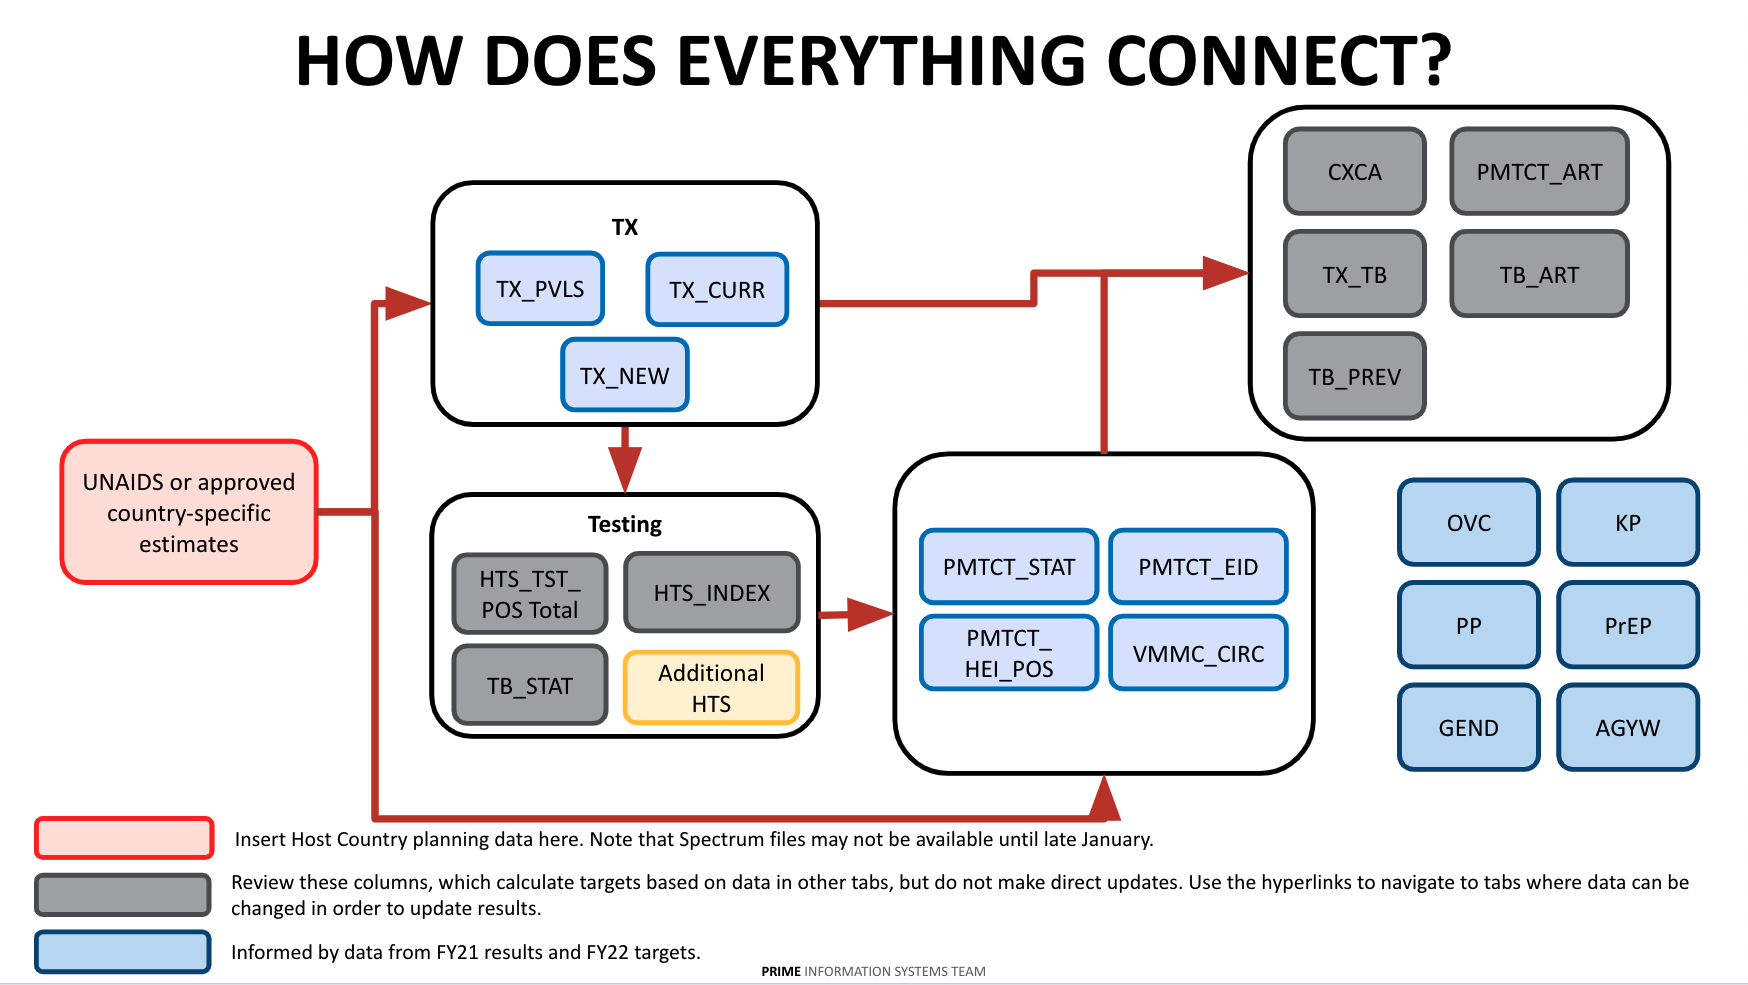
\includegraphics[width=9in]{images/UG_Sec 1-6 How Does Everything Connect.png}

\end{center}

\newpage

\hypertarget{elements-of-a-tab}{%
\section{Elements of a Tab}\label{elements-of-a-tab}}

\begin{center}

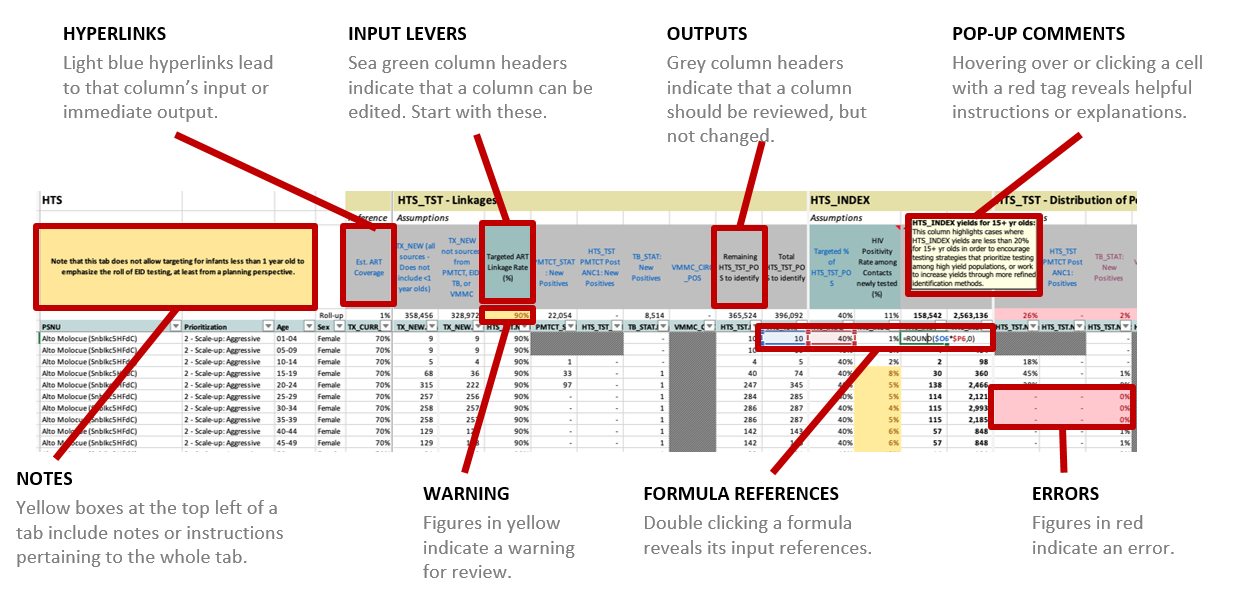
\includegraphics[width=9in]{./images/image4.png}

\end{center}

\newpage

\hypertarget{how-to-navigate-a-datapack-tab}{%
\section{How to Navigate a DataPack Tab}\label{how-to-navigate-a-datapack-tab}}

\begin{center}

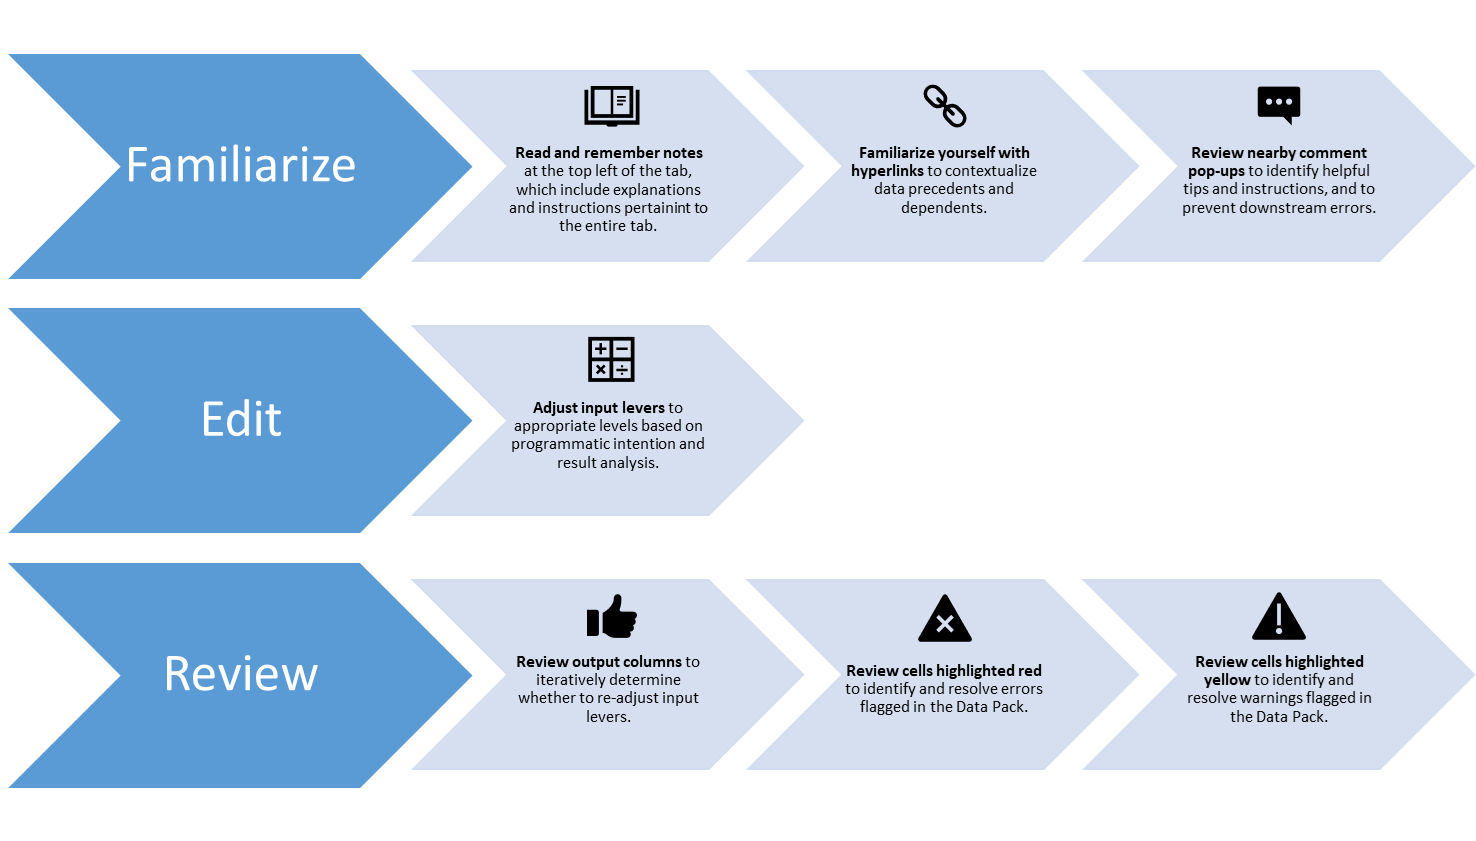
\includegraphics[width=9in]{./images/image5.png}

\end{center}

\elandscape

\newpage

\textbf{ENTERING DATA IN THE CORRECT SECTION}

In the tabs for the DATIM Data Elements, sections may either have data
prepopulated from DATIM or the user will enter data into that column.
Each section of the guide will list what columns users can expect to
have data prepopulated and / or where they can enter data themselves.

\textbf{ENTERING DATA IN THE WRONG SECTION}

If you enter data into a cell that you are not supposed to enter data
into, you will receive the following message box with corrective action
suggestions as well.

\textbf{Example:}

\begin{center}

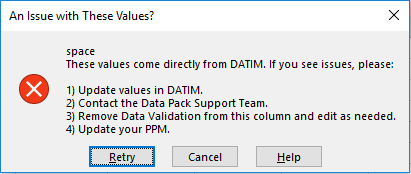
\includegraphics[width=4.3in]{./images/image9.png}

\end{center}

\hypertarget{adjustments-to-historic-targets-and-results}{%
\section{Adjustments to Historic Targets and Results}\label{adjustments-to-historic-targets-and-results}}

Throughout the DataPack, historic targets and results have been provided
for reference and often to drive target modeling algorithms. If, in the
process of reviewing these historic data, issues with the data are
discovered that may need to be addressed in DATIM, follow the below
procedure:

\begin{enumerate}
\def\labelenumi{\arabic{enumi}.}
\item
  Raise specific issues with historic data to your PPM and DUIT
  Liaison. Determine together whether any issue identified requires
  updating values in DATIM.
\item
  It maybe that together with your PPM and DUIT Liaison you decide
  that changes to historic values are not necessary in DATIM, but
  still necessary in the DataPack. This is an extraordinary
  circumstance and must have approval from PRIME/DUIT leadership via
  your Liaison to allow. If approved, you may make changes directly in
  the related column of the DataPack.
\item
  If it is the case that DATIM values should be updated, follow the
  usual process for OPU Target changes, requesting all necessary
  approvals to initiate and expedite this process during COP.
\item
  Once changes are aprroved, either through an OPU for targets, or
  through data change request for results, you can enter the new
  values into the related column of the DataPack yourself. If you wish
  to request a new DataPack, you may do so, but will have to start the
  DataPack process afresh. For either of these routes, reach out to
  the DataPack Systems Team via Zendesk for support.
\end{enumerate}

\newpage

\hypertarget{release-notes}{%
\chapter{Release Notes}\label{release-notes}}

\hypertarget{datapackr-5.0.3}{%
\section{datapackr 5.0.3}\label{datapackr-5.0.3}}

\hypertarget{new-features}{%
\subsection{New features}\label{new-features}}

\begin{itemize}
\tightlist
\item
  Initial launch of COP22 Data Pack processing!
\end{itemize}

\hypertarget{breaking-changes}{%
\subsection{Breaking changes}\label{breaking-changes}}

\begin{itemize}
\tightlist
\item
  Now requires R version 4.1.1 or higher.
\end{itemize}

\hypertarget{minor-improvements-and-fixes}{%
\subsection{Minor improvements and fixes}\label{minor-improvements-and-fixes}}

\begin{itemize}
\tightlist
\item
  Updated and improved documentation of datasets in \texttt{datapackr}.
\item
  Improves handling of default \texttt{categoryOptionCombo}.
\item
  Improves documentation of \texttt{packDataPackSheet}, \texttt{packSheets}, and \texttt{prepareSheetData}.
\end{itemize}

\hypertarget{deprecated-features}{%
\subsection{Deprecated features}\label{deprecated-features}}

\begin{itemize}
\tightlist
\item
  \texttt{loginToDATIM} is retired in favor of the same function in \texttt{datimutils}. All
  instances of this function being invoked have been replaced appropriately.

  \begin{itemize}
  \tightlist
  \item
    The functions \texttt{DHISLogin}, \texttt{GetCredentialsFromConsole}, \texttt{LoadConfigFile},
    and \texttt{ValidateConfig} were not exported and are now deprecated as well.
    They were previously only used by \texttt{loginToDATIM}.
  \end{itemize}
\item
  \texttt{isLoggedIn} is retired as it was only used in \texttt{getMechList} and
  \texttt{loginToDATIM}.
\end{itemize}

\hypertarget{datapackr-5.0.2}{%
\section{datapackr 5.0.2}\label{datapackr-5.0.2}}

\hypertarget{bug-fixes}{%
\subsection{Bug fixes}\label{bug-fixes}}

\begin{itemize}
\tightlist
\item
  Resolves a bug with \texttt{packOPUDataPack} where \texttt{createDataPack} was not
  implemented correctly in version 5.0.1.
\item
  Patches a bug with \texttt{getOPUDataFromDATIM} where \texttt{getCOPDataFromDATIM} returns
  a dataframe where the default Category Option Combo UID is listed as \texttt{default}
  rather than the appropriate DATIM UID. This will be removed in favor of a more
  permanent solution in future updates.
\end{itemize}

\hypertarget{new-features-1}{%
\subsection{New features}\label{new-features-1}}

\begin{itemize}
\tightlist
\item
  Significantly improves handling of parameter checks and standardizes their
  validation and defaults. Documentation for these checks is also added.
\item
  Adds functionality for producing COP22 Beta Packs and test data.
\end{itemize}

\hypertarget{breaking-changes-1}{%
\subsection{Breaking changes}\label{breaking-changes-1}}

\begin{itemize}
\tightlist
\item
  Removes \texttt{getDataPackSchema} in favor of consolidated \texttt{pick\_schema}.
\end{itemize}

\hypertarget{deprecated-features-1}{%
\subsection{Deprecated features}\label{deprecated-features-1}}

\begin{itemize}
\tightlist
\item
  \texttt{getDataPackSchema} has been deprecated in favor of \texttt{pick\_schema} and has been
  replaced in the two locations where it was previously used.
\end{itemize}

\hypertarget{minor-improvements-and-fixes-1}{%
\subsection{Minor improvements and fixes}\label{minor-improvements-and-fixes-1}}

\begin{itemize}
\tightlist
\item
  Improves and updates tests related to parameter checks and schemas.
\item
  Introduces many new small utilities functions such as \texttt{\%missing\%} and \texttt{\%\textbar{}\textbar{}\%}.
\item
  Improves automation of Data Pack Template/schema validation.
\end{itemize}

\hypertarget{datapackr-5.0.1}{%
\section{datapackr 5.0.1}\label{datapackr-5.0.1}}

\hypertarget{new-features-2}{%
\subsection{New features}\label{new-features-2}}

\begin{itemize}
\tightlist
\item
  \texttt{loadDataPack} is a new function that returns a Data Pack object conserving
  styles and formatting of the original Data Pack .xlsx file, as well as other
  metadata necessary for processing and analysing data in the Data Pack.
\item
  \texttt{.testInvalidIndicatorCodes} was previously an internal function that is now
  documented and exported by the package. This function tests for invalid
  indicator codes in a \texttt{d} Datapackr object.
\item
  \texttt{datapack\_cogs} is a new dataset containing Datapack Category option groups
  (id and name) along with their individual category options (id and name) as a
  nested data frame.
\end{itemize}

\hypertarget{breaking-changes-2}{%
\subsection{Breaking changes}\label{breaking-changes-2}}

\begin{itemize}
\tightlist
\item
  \texttt{createWorkbook} has been renamed \texttt{createDataPack} to deconflict with the
  openxlsx function \texttt{createWorkbook}. This function now returns a \texttt{d}
  datapackr object rather than an openxlsx workbook object.
\item
  The \texttt{d2\_session} argument has been removed from the following functions:

  \begin{itemize}
  \tightlist
  \item
    \texttt{check\_params}
  \item
    \texttt{createDataPack} (previously \texttt{createWorkbook})
  \item
    \texttt{unPackSchema\_datapack}
  \end{itemize}
\end{itemize}

\hypertarget{minor-improvements-and-fixes-2}{%
\subsection{Minor improvements and fixes}\label{minor-improvements-and-fixes-2}}

\begin{itemize}
\tightlist
\item
  \texttt{unPackSchema\_datapack} was modified in the following ways:

  \begin{itemize}
  \tightlist
  \item
    Now uses the \texttt{datapack\_cogs} data set rather than making a query to DATIM.
  \item
    Inherits parameters from \texttt{datapackr\_params}.
  \end{itemize}
\item
  \texttt{writeHomeTab} was modified in the following ways:

  \begin{itemize}
  \tightlist
  \item
    The \texttt{wb} and \texttt{datapack\_name} arguments default to \texttt{NULL}.
  \item
    Checks and assigns parameters using the \texttt{check\_params} function.
  \item
    Lists country names on the Home tab in addition to Country UIDs.
  \end{itemize}
\item
  Minor corrections were made to Excel functions written by \texttt{packSNUxIM} that
  had been erroneously changed during previous linting.
\item
  Internal changes were made to variable names and functions used inside the
  \texttt{check\_params} function.
\item
  A new file has been added to \texttt{data-raw} to generate the \texttt{datapack\_cogs}
  data set.
\item
  Documentation is now provided for the \texttt{cop20OPU\_data\_pack\_schema} data set.
\end{itemize}

\hypertarget{whats-new}{%
\chapter{What's New?}\label{whats-new}}

\hypertarget{section-7-changes}{%
\subsubsection{Section 7 Changes}\label{section-7-changes}}

\textbf{Reorienting of the Cascade Tab around PVLS}, rather than ART Coverage, although both are taken into account. This year's new shift to begin setting the Cascade from Program Viral Load Suppression. This starting point will allow for country team users to build up a full cascade that will provide insight into VLS, VL Testing and how this will translate into determining the new on treatment and those returning to treatment. It will provide a full picture of the treatment ecosystem and the way in which countries understand if they will achieve 85\% coverage across all three Cascades. This will allow countries that are at or close to Epidemic Control to better approach the understanding of how they will continue to sustain their 95-95-95 goals. This approach will put a greater emphasis on the Coverage Cascade as the driver of the target setting process, a direct shift from the past 5 years that have focused on the first two Cascades, and paint a picture of both VL to gap in Treatment and Testing.

\hypertarget{mer2.6-changes}{%
\subsubsection{MER2.6 Changes}\label{mer2.6-changes}}

\textbf{Changes in line with MER 2.6}:

\begin{itemize}
\item
  Use of PrEP\_CT in lieu of PrEP\_CURR.
\item
  Integration of the new SNS modality.
\item
  50+ finer age bands across the clinical cascade. These will be aggregated to 50+ upon DATIM import for all but TX\_CURR.
\end{itemize}

The introduction of 65+ age bands for TX\_CURR targets this year will be visible across the Cascade, PMTCT, TB, and VMMC tabs. For structural purposes of these tabs to seamlessly work with the new inclusion of the 50+ finer age bands, targets will be set across many indicators at the finer age bands across the clinical cascade. The most important thing for users to note is that these will be aggregated to 50+ upon DATIM import for all but TX\_CURR. The breakdown that has been used to disaggregate the 50+ age band into the finer age bands up to 65+ is the following:

\begin{itemize}
\item
  50-54: 42\%
\item
  55-59: 35\%
\item
  60-64 14\%
\item
  65+: 9\%
\end{itemize}

These percentages were determined through various research studies. If teams feel as though they need to adjust the breakdowns based on local data and research they are able to do so, but should first consult their Chair, PPM and DUIT Liaison.

\hypertarget{psnuxim-tool-formulas}{%
\subsubsection{\texorpdfstring{\textbf{PSNUxIM Tool Formulas}}{PSNUxIM Tool Formulas}}\label{psnuxim-tool-formulas}}

The PSNUxIM tab will now be split into its own separate tool. When you received your newly generated PSNUxIM tool for the first time, you will need to scroll to the ``Target Values'' Section that begins in column CW and copy down the formulas populated in row 15 all the way down to the bottom of your DataPack. This will be required in order for your Rollup column to properly populate as well as the Deduplication sections.

\hypertarget{frequently-asked-questions}{%
\chapter{Frequently Asked Questions}\label{frequently-asked-questions}}

\textbf{\emph{Q: Why are there more than just TX\_CURR (FY23) Indicators being set at the new finer 65+ age bands despite MER2.6 Guidance?}}

A: Due to the structure of the Cascade tab, and other COP22 - FY23 Targets that rely on TX\_CURR (FY23), the tool had to be built, such that these tabs are all disaggregated to the the 65+ age band. However, upon completion of the DataPack, ONLY TX\_CURR (FY23) will be import to DATIM with the finer age bands. All other indicators will be aggregated to 50+.

\textbf{\emph{Q: When working through PSNUxIM KP mechanism allocations and I allocate the KP-specific targets to KP partners, given that the KP disaggregates are a subset of the total population being targeted, do I also need to allocate total pop targets to the KP partner?}}

A: Yes, you should be setting a corresponding Total Pop target against each mechanism you set KeyPop targets against. This is because KeyPop is a subset of Total Pop. Note however, that only clinical, facility partners may have targets and report many indicators. For these indicators, the KP targets must be assigned to a partner and site qualified to report the results.

\textbf{\emph{Q: Can you use FY23 Spectrum estimates to work through the Cascade tab?}}

A: No, unless you receive approval from OGAC Leadership you should use FY22 Spectrum Data. Your target setting process for the COP22 DataPack should be to set FY23 targets based on where you are ending FY22.

\textbf{\emph{Q: Is the coverage rate that is used to calculate ``Targeted Host Country TX\_CURR\_SUBNAT (FY22)'' and ``Targeted Host Country TX\_NET\_NEW\_SUBNAT (FY22)'' too high or being miscalculated?}}

A: No, this is not a formula error. The calculations occurring are focusing on PLHIV for each district that are being treated for HIV/AIDS for each age band, as opposed to those being treated for HIV/AIDS in the district regardless of whether they live in that district. if the PEPFAR results are higher than the PLHIV Spectrum estimate in a particular district, then back-calculating the coverage rate shows a greater than 100\% value for that PSNU-Age-Sex band. This can come from one of two things generally: People are coming from outside the district to seek treatment, leading to a higher PEPFAR TX\_CURR value than PLHIV in the district; or The PLHIV estimate from Spectrum is too low. Either way if you have good programmatic reason for doing so, particularly health seeking behavior of PLHIV, you can aim for a coverage rate even higher than 100\% (e.g., current coverage in capital city is estimated at 105\%, but due to health seeking behavior you want to aim for 120\% to achieve 95\% for across all metropolitan area).

\textbf{\emph{Q: Why in the newly generated PSNUxIM tab are data-pack totals and roll up columns blank?}}

A: Once you have regenerated your PSNUxIM tab from the DataPack Self-Service app, please open your newly regenerated tool, save your tool and close it. When you reopen your tool, it should populate your targets into that column. You will also need to drag down the formula in the far right ``Target Values'' section of the PSNUxIM tab to ensure all rows are populated with the proper formula.

\textbf{\emph{Q: If my program performs testing but not treatment, how do I represent this in the DataPack?}}

A: You will first need approval from OGAC Leadership to do this. If you receive this approval you will need to manually alter in the Cascade Tab column ``HTS\_TST\_POS + PMTCT\_HEI\_POS (FY22)'' (BD). Please make the alterations to this column and not on the HTS tab.

\textbf{\emph{Q: When I try to validate my DataPack in the self-service app, I get a message saying ``ERROR: An error has occurred. Check your logs or contact the app author for clarification.'' How do I resolve this?}}

A: This error can be caused by a number of different issues. The most common causes and their resolutions include:

\begin{itemize}
\tightlist
\item
  Trying to validate a newly regenerated DataPack before opening it and saving it. After generating or regenerating your PSNUxIM tab, it is necessary to first open your tool and save it before uploading it to the app.
\item
  The browser is causing issues with the app. This can be resolved by opening an Incognito window or by clearing your cache. PLEASE NOTE: Clearing your cache will sign you out of all accounts in that browser.
\item
  Trying to validate a file that isn't an XLSX. If your team has saved your DataPack in a different file format for sharing, such as XLSB, ensure that you resave the file as an XLSX before validating it in the app.
\item
  The target distribution formulas on the PSNUxIM tab have not been applied to all rows. By default, the formulas in the ``Target Value'' section (Column CW and right) are only applied to Row 15. Once you generate or regenerate your PSNUxIM tab, ensure that you copy these formulas all the way down to the bottom row of your targets. After this is done, try validating your tool again.
\end{itemize}

If none of the above issues apply to your DataPack tool and you are still receiving this error, please submit a ZenDesk ticket identifying your country and attaching or linking to a copy of the DataPack tool that caused the error in the app.

\hypertarget{testing-targets-cheat-sheet}{%
\chapter{Testing Targets Cheat Sheet}\label{testing-targets-cheat-sheet}}

\hypertarget{purpose}{%
\section{Purpose}\label{purpose}}

The purpose of this cheat sheet is to document a recurring DataPack issue to guide other OU's towards a solution. This document does not supersede PEPFAR guidance. For more questions, please contact the ICPI Zendesk.

\hypertarget{issue}{%
\section{Issue}\label{issue}}

Our HTS\_TST\_POS targets from modalities are summing to over 100\% of the HTS\_TST\_POS total. We have too many positives but cannot figure out how to resolve the errors in the datapack?

\hypertarget{is-this-issue-in-my-datapack}{%
\section{Is this issue in my DataPack?}\label{is-this-issue-in-my-datapack}}

This issue is most likely to affect countries with high treatment coverage but has been seen in lower coverage OUs as well

\begin{itemize}
\tightlist
\item
  If your DataPack has negative values in the Other Modalities \textbf{(Cascade Tab; Column BR)} or a large HTS POS difference to adjust \textbf{(HTS Tab; Column BO)}
\end{itemize}

\textbf{\emph{AND}}

\begin{itemize}
\tightlist
\item
  You have already walked through the instructions in the Datapack User Guide HTS Section link \href{https://apps.datim.org/datapack-userguide/15-HTS.html}{HERE}
\end{itemize}

\hypertarget{why-is-this-issue-in-my-datapack}{%
\section{Why is this issue in my DataPack?}\label{why-is-this-issue-in-my-datapack}}

\begin{itemize}
\tightlist
\item
  COP guidance recommends that age/sex/SNU combinations with high treatment coverage (above 80\%) have a high rate of positives (75\%) coming from index testing, but countries may already have more than 25\% of positives coming from other passive modalities (PMTCT, TB).
\item
  Countries with lower treatment coverage will have different recommendations for positives from index testing; See figure 2.3.2.2 on page 66 of the COP guidance for more details. Even in settings with only 30\% of positives coming from index testing you may still see this issue.
\end{itemize}

\hypertarget{possible-solutions}{%
\section{Possible solutions}\label{possible-solutions}}

\begin{itemize}
\item
  Work with your PMTCT and TB program colleagues to review your program and surveillance data and increase the percentage of known positives coming from PMTCT (and other modalities, such as TB and VMMC)

  \begin{itemize}
  \tightlist
  \item
    Changes in PMTCT are most likely to decrease high positives (while maintaining ambitious targets for your PMTCT program)
  \item
    See examples below for PMTCT and TB indicators
  \end{itemize}
\item
  If still unable to resolve high positives, need to ask permission from SGAC Chair, PPM, and DUIT liaisons to change underlying assumptions set by COP Guidance, such as \% of positives that come from Index Testing

  \begin{itemize}
  \tightlist
  \item
    Be prepared to share what the value should be and provide justification
  \item
    For example, in one Operating Unit, PEPFAR has already transitioned all funding lower yield provider-initiated testing (PITC) to the Ministry of Health (through Global Fund support); despite being lower yield these modalities still identify approximately 50\% of positives needed to be identified at PEPFAR supported sites; it is, therefore, not possible to obtain 75\% positives from PEPFAR supported index testing
  \end{itemize}
\end{itemize}

\hypertarget{how-to-try-these-solutions-in-the-datapack}{%
\section{How to try these solutions in the DataPack}\label{how-to-try-these-solutions-in-the-datapack}}

Remember that you can only change the sea green columns in the DP. The following solutions are in order of impact (high to low).

\hypertarget{pmtct-tab---decrease-positives-from-anc-and-post-anc1}{%
\subsection{PMTCT Tab - decrease positives from ANC and Post-ANC1}\label{pmtct-tab---decrease-positives-from-anc-and-post-anc1}}

\textbf{Goal: To reduce column AE ``Newly Tested, Positive'' which feeds into the total HTS\_TST\_POS values that are too high}

\begin{itemize}
\item
  Shift positives from newly tested to known positives
\item
  \textbf{Column Z} ``Est. \% ANC1 clients already Known HIV Positive (\%)''

  \begin{itemize}
  \tightlist
  \item
    Increasing column Z directly increases column AD ``Known HIV Status, Positive'' by the same amount it decreases column AF ``Newly Tested, Negative'' ultimate reducing ``Newly Tested Positives''
  \item
    This reduction in New Positives may be small
  \end{itemize}
\item
  \textbf{Column AB} ``Est. Positivity Rate among Newly Tested ANC1 clients (\%)''

  \begin{itemize}
  \tightlist
  \item
    Decreasing column AB directly decreases column AE ``Newly Tested, Positive'' by the same amount it decreases column AF ``Newly Tested, Negative''
  \item
    This reduction in Newly Tested Positives will be bigger, proceed with caution
  \end{itemize}
\end{itemize}

\begin{center}

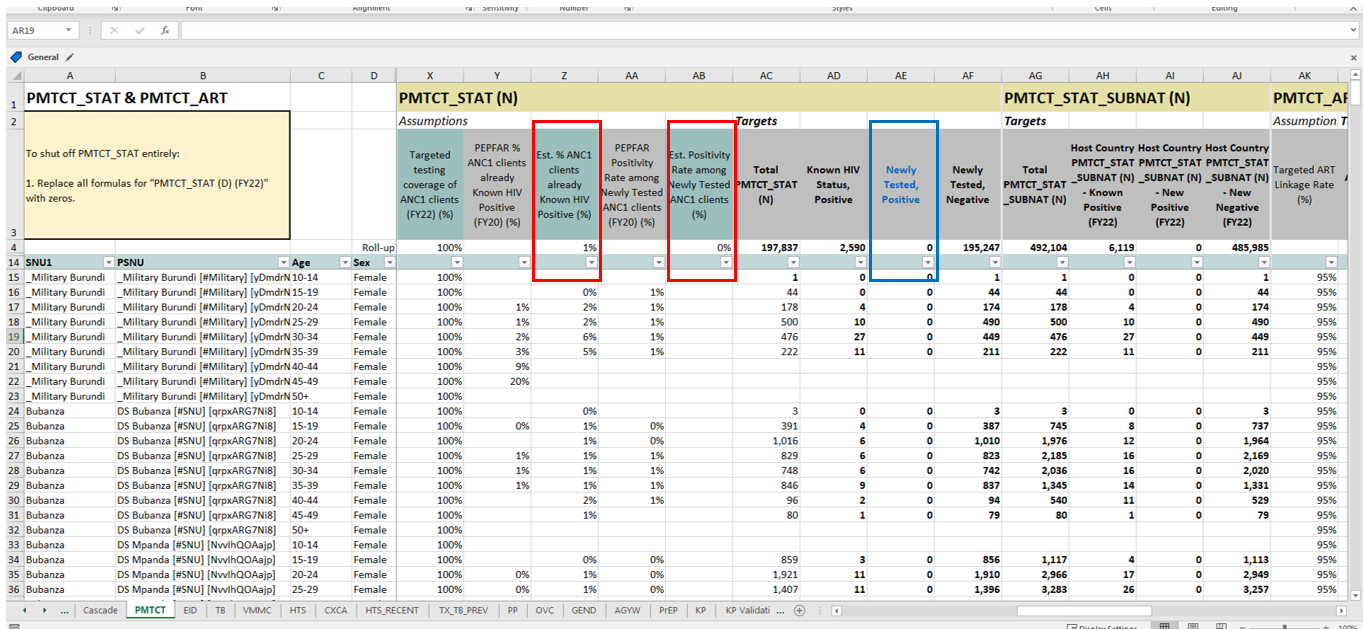
\includegraphics[width=7in]{./images/image16.png}

\end{center}

\textbf{Goal: To reduce Column AU ``Positives'' from Post ANC1}

\begin{itemize}
\item
  This change will most likely only have a small impact on your total positives
\item
  Increasing Known Positives (in step above) reduces Column AQ ``Total eligible for Post ANC1 retesting'' thereby reducing column AU ``Positive''
\item
  \textbf{Column AS ``Yield (\%)''}

  \begin{itemize}
  \tightlist
  \item
    Reducing Yield will reduce Positive (AU)
  \item
    While it is not plausible to see no positives from Post ANC1, consider a programmatic maximum that you would like to target
  \end{itemize}
\item
  While it is possible to change Column AQ, we recommend not altering this column directly so as to not create logical gaps in PMTCT testing process
\end{itemize}

\begin{center}

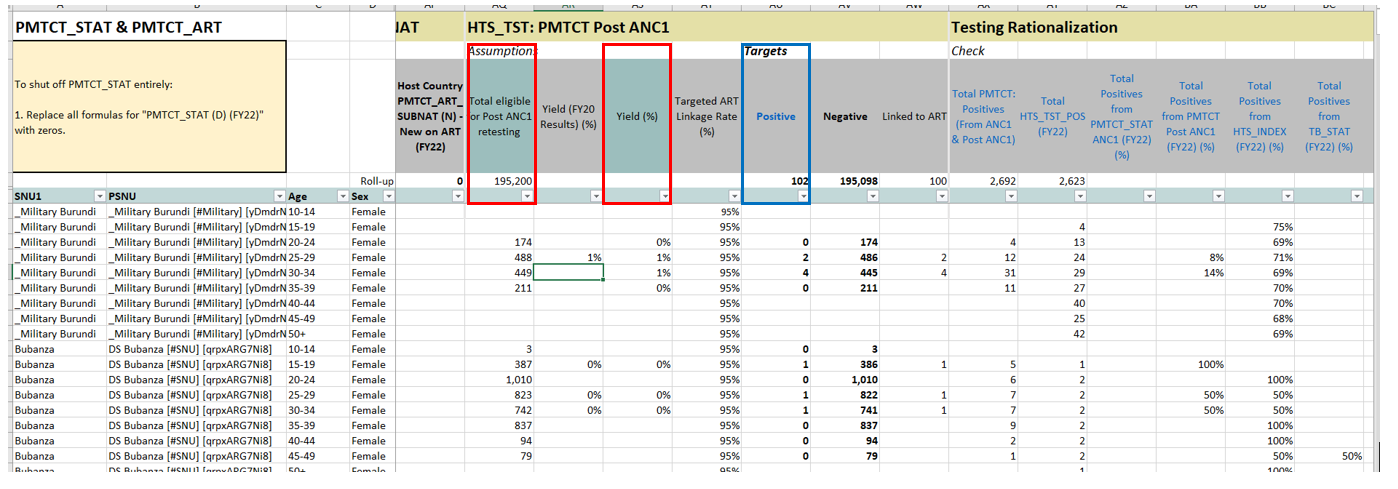
\includegraphics[width=7in]{./images/image17.png}

\end{center}

\hypertarget{tb-tab---decrease-positives-from-tb}{%
\subsection{TB tab - decrease positives from TB}\label{tb-tab---decrease-positives-from-tb}}

\textbf{Goal: To reduce column Q ``Newly Tested, Positive'' which feeds into the total HTS\_TST\_POS values that are too high}

\begin{itemize}
\item
  Shift positives from newly tested to known positives
\item
  \textbf{Column L} ``Est. \% TB clients already Known HIV Positive (\%)''

  \begin{itemize}
  \tightlist
  \item
    Increasing column L directly increases column P ``Known HIV Status, Positive'' by the same amount it decreases column R ``Newly Tested, Negative'' ultimate reducing ``Newly Tested Positives''
  \item
    This reduction in New Positives may be small
  \end{itemize}
\item
  \textbf{Column N} ``Est. Positivity Rate among Newly Tested (\%)''

  \begin{itemize}
  \tightlist
  \item
    Decreasing column N directly decreases column Q ``Newly Tested, Positive'' by the same amount it decreases column R ``Newly Tested, Negative''
  \item
    This reduction in Newly Tested Positives will be bigger, proceed with caution
  \end{itemize}
\end{itemize}

\begin{center}

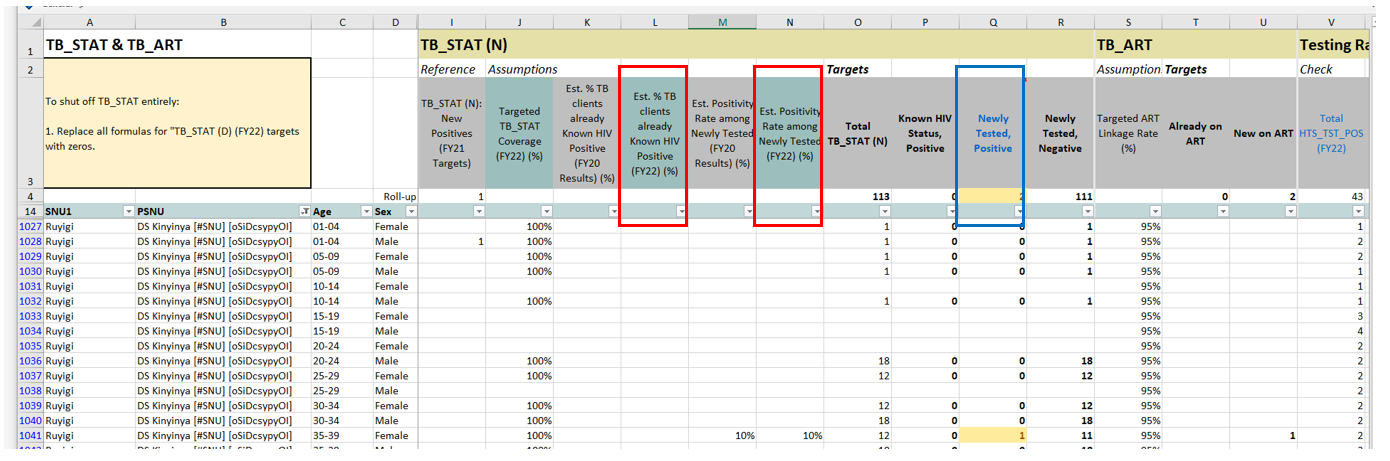
\includegraphics[width=7in]{./images/image18.png}

\end{center}

\blandscape

\hypertarget{how-to-fill-out-the-datapack}{%
\chapter{How to Fill Out the DataPack}\label{how-to-fill-out-the-datapack}}

\begin{center}

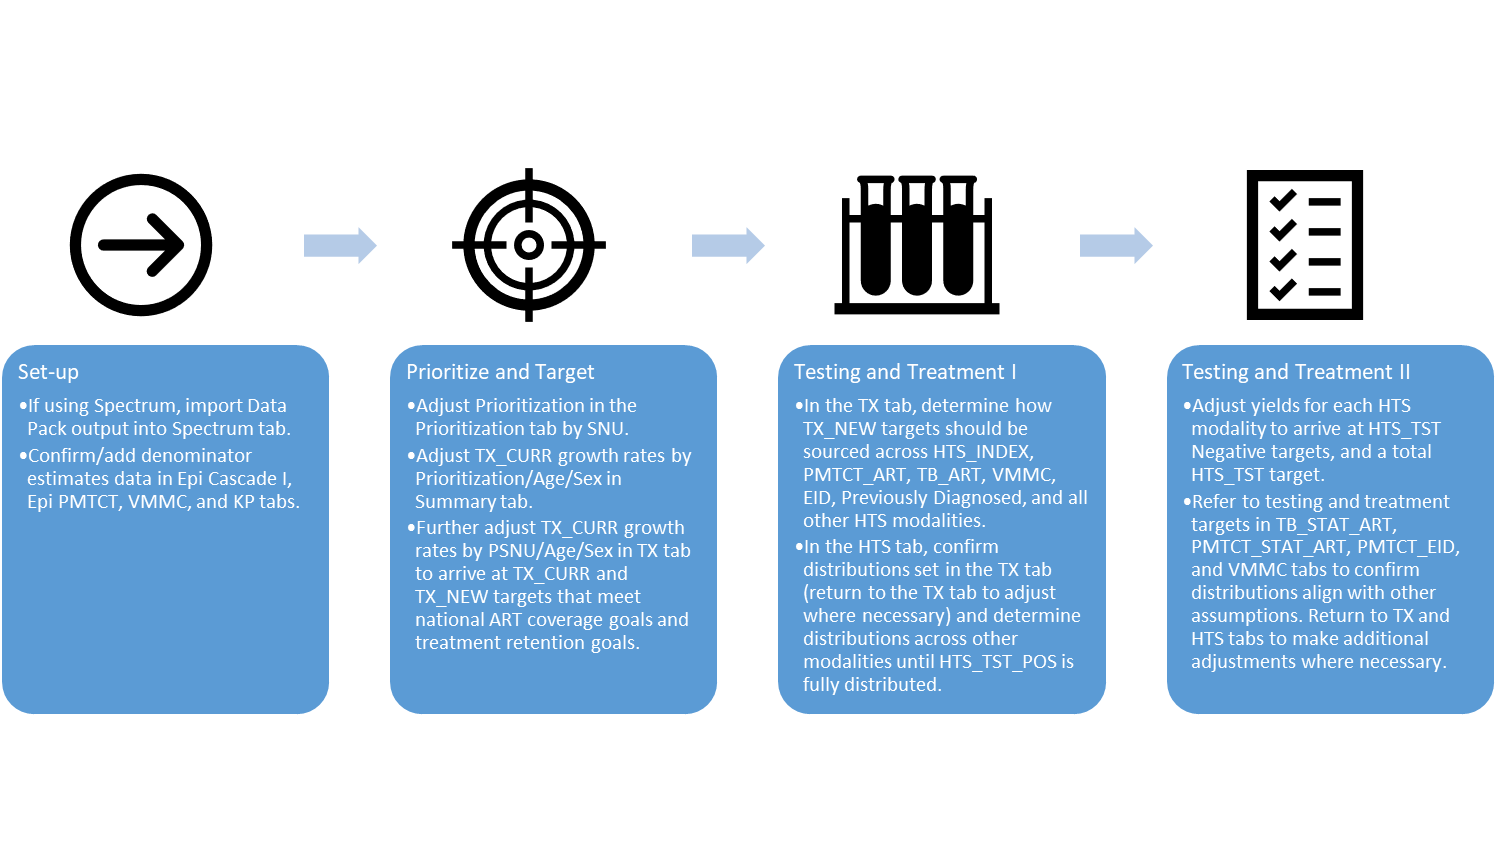
\includegraphics[width=9in]{./images/image12.png}

\end{center}

\newpage

\begin{center}

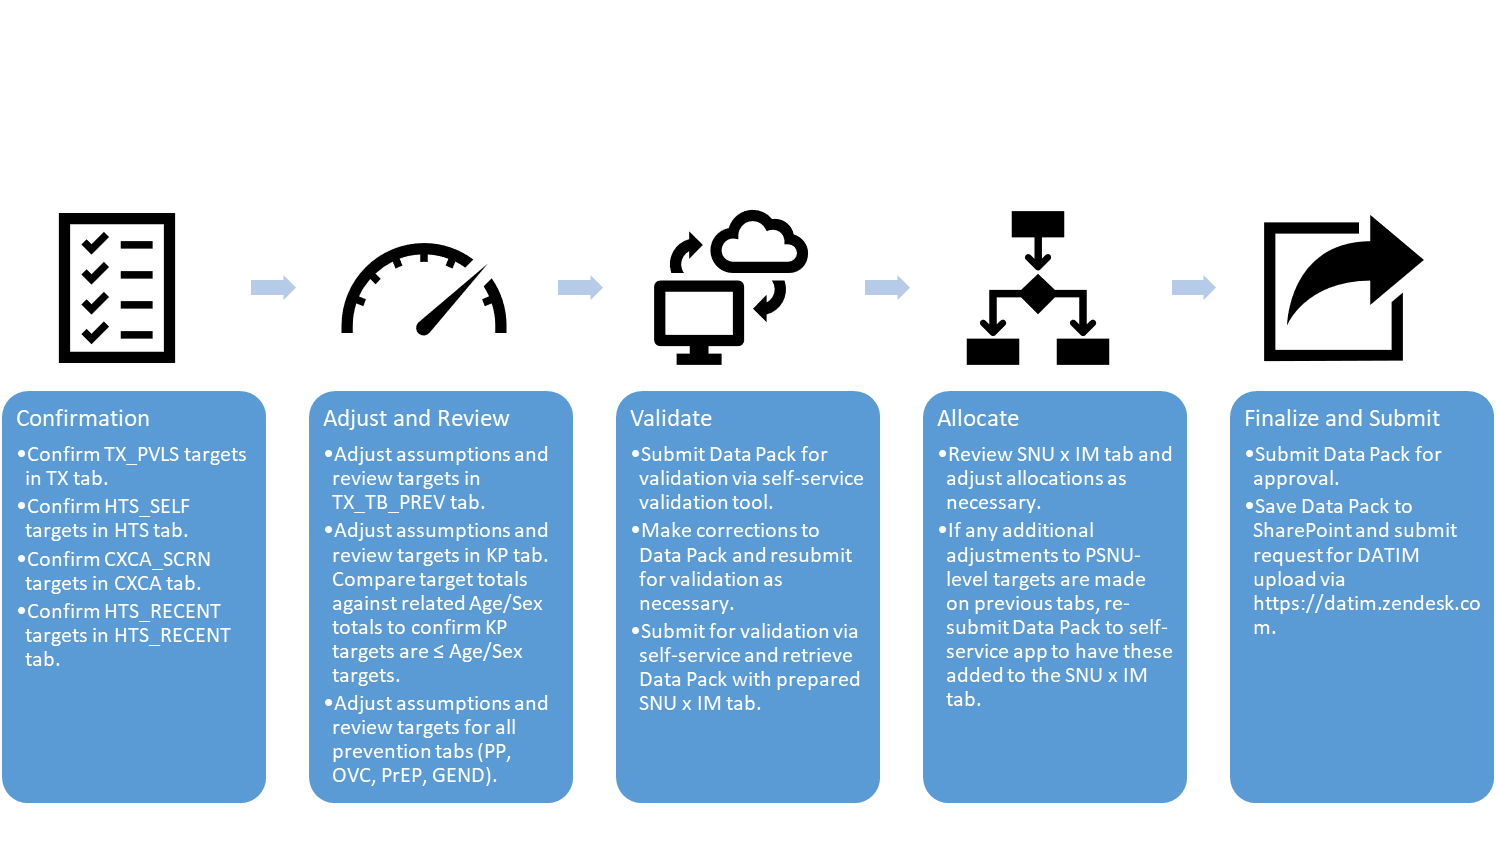
\includegraphics[width=9in]{./images/image13.png}

\end{center}

\elandscape

\newpage

\hypertarget{how-to-use-the-user-manual}{%
\chapter{How to Use the User Manual}\label{how-to-use-the-user-manual}}

The DataPack consists of tabs that address indicators related to each
PEPFAR program area.

The COP22 DataPack User Manual reviews all indicators within each tab
and provides you with the relevant information to complete all required
sections of the DataPack correctly. It also instructs you where to find
more information on each program area in the COP21 Guidance.

\hypertarget{key-column-highlights}{%
\section{Key Column Highlights}\label{key-column-highlights}}

\begin{quote}
\textbf{\emph{Column type?}} Indicates whether the data in this column is a
result from a previous fiscal year (``Result''), an assumption that the
country team is making (``Assumption''), a target for FY2023
(``Targets''), or a reference for the country team as they fill out the
DataPack (``Reference'').

\textbf{\emph{What type of data?}} Indicates whether the data in the column is
an integer, e.g., a whole number, or a percentage.

\textbf{\emph{Prepopulated data?}} Indicates whether the data in this column is
prepopulated from data in DATIM or from data elsewhere in the
DataPack.

\textbf{\emph{Enter or modify data?}} Indicates whether the user should enter
new information into this column or is allowed to modify the
prepopulated information in the column. If there is a question mark
here, country teams must consult with their PPMs and Chairs before
modifying the data in this column. If there is an exclamation mark
here, country teams may overwrite the formula in this column, however
it will prevent the DataPack from refreshing this data if changes are
made elsewhere.

\textbf{\emph{Calculated column?}} This indicates that a formula is used to
indicate where a formula is used to calculate the values in this
column from data elsewhere in the DataPack.

\textbf{\emph{Linked column?}} This indicates that this data is either
prepopulated by or is used to prepopulate data in a column on another
tab within the DataPack. For columns that are prepopulated from
another tab, clicking on the hyperlinked column name in the DataPack
will take you to the referenced column.

\emph{\textbf{UID in Appendix}.} The UID provided here is a DataPack reference
ID and can be used to find more information about the data entered
into this column in the appendices.
\end{quote}

\newpage

\blandscape

\hypertarget{spectrum}{%
\chapter{SPECTRUM}\label{spectrum}}

The Spectrum tab will allow users to load UNAIDS data with 12 columns of data elements for your OU. A Spectrum file for your OU will be provided at the conclusion of the UNAIDS Spectrum Training for Country Teams. The contents of this file will be manually loaded into the Spectrum tab which is setup as below:

\begin{table}
\centering\begingroup\fontsize{12}{14}\selectfont

\resizebox{\linewidth}{!}{
\begin{tabular}{>{\raggedright\arraybackslash}p{1.25in}>{\raggedright\arraybackslash}p{1.25in}>{\raggedright\arraybackslash}p{1.25in}>{\raggedright\arraybackslash}p{1.25in}>{\raggedright\arraybackslash}p{1.25in}>{\raggedright\arraybackslash}p{1.25in}l}
\toprule
\multicolumn{1}{>{\centering\arraybackslash}p{1.25in}}{\cellcolor[HTML]{E6DFA7}{name}} & \multicolumn{1}{>{\centering\arraybackslash}p{1.25in}}{\cellcolor[HTML]{E6DFA7}{D}} & \multicolumn{1}{>{\centering\arraybackslash}p{1.25in}}{\cellcolor[HTML]{E6DFA7}{E}} & \multicolumn{1}{>{\centering\arraybackslash}p{1.25in}}{\cellcolor[HTML]{E6DFA7}{F}} & \multicolumn{1}{>{\centering\arraybackslash}p{1.25in}}{\cellcolor[HTML]{E6DFA7}{G}} & \multicolumn{1}{>{\centering\arraybackslash}p{1.25in}}{\cellcolor[HTML]{E6DFA7}{H}} & \multicolumn{1}{c}{\cellcolor[HTML]{E6DFA7}{I}}\\
\midrule
Column Name & psnu & psnu\_uid & area\_id & indicator\_code & dataelement\_uid & age\\
Column Type? & NA & NA & NA & NA & NA & NA\\
What type of data? & string & string & string & string & string & string\\
Prepopulated data? & N & N & N & N & N & N\\
Enter or modify data? & Y & Y & Y & Y & Y & Y\\
\addlinespace
Calculated column? & N & N & N & N & N & N\\
Linked column? & N & N & N & N & N & N\\
\bottomrule
\end{tabular}}
\endgroup{}
\end{table}

\begin{table}
\centering\begingroup\fontsize{12}{14}\selectfont

\resizebox{\linewidth}{!}{
\begin{tabular}{>{\raggedright\arraybackslash}p{1.07142857142857in}>{\raggedright\arraybackslash}p{1.07142857142857in}>{\raggedright\arraybackslash}p{1.07142857142857in}>{\raggedright\arraybackslash}p{1.07142857142857in}>{\raggedright\arraybackslash}p{1.07142857142857in}>{\raggedright\arraybackslash}p{1.07142857142857in}>{\raggedright\arraybackslash}p{1.07142857142857in}l}
\toprule
\multicolumn{1}{>{\centering\arraybackslash}p{1.07142857142857in}}{\cellcolor[HTML]{E6DFA7}{name}} & \multicolumn{1}{>{\centering\arraybackslash}p{1.07142857142857in}}{\cellcolor[HTML]{E6DFA7}{J}} & \multicolumn{1}{>{\centering\arraybackslash}p{1.07142857142857in}}{\cellcolor[HTML]{E6DFA7}{K}} & \multicolumn{1}{>{\centering\arraybackslash}p{1.07142857142857in}}{\cellcolor[HTML]{E6DFA7}{L}} & \multicolumn{1}{>{\centering\arraybackslash}p{1.07142857142857in}}{\cellcolor[HTML]{E6DFA7}{M}} & \multicolumn{1}{>{\centering\arraybackslash}p{1.07142857142857in}}{\cellcolor[HTML]{E6DFA7}{N}} & \multicolumn{1}{>{\centering\arraybackslash}p{1.07142857142857in}}{\cellcolor[HTML]{E6DFA7}{O}} & \multicolumn{1}{c}{\cellcolor[HTML]{E6DFA7}{P}}\\
\midrule
Column Name & age\_uid & sex & sex\_uid & calendar\_quarter & value & age\_sex\_rse & district\_rse\\
Column Type? & NA & NA & NA & NA & NA & NA & NA\\
What type of data? & string & string & string & string & integer & percentage & percentage\\
Prepopulated data? & N & N & N & N & N & N & N\\
Enter or modify data? & Y & Y & Y & Y & Y & Y & Y\\
\addlinespace
Calculated column? & N & N & N & N & N & N & N\\
Linked column? & N & N & N & N & N & N & N\\
\bottomrule
\end{tabular}}
\endgroup{}
\end{table}

With OGAC approval, countries can also populate input their own data into this tab with a different MOH/country approved set of estimates. Estimate changes can also be made in the two associated tabs, Cascade and PMTCT.

\elandscape

\newpage

\blandscape

\hypertarget{prioritization}{%
\chapter{PRIORITIZATION}\label{prioritization}}

\begin{table}
\centering\begingroup\fontsize{12}{14}\selectfont

\resizebox{\linewidth}{!}{
\begin{tabular}{>{\raggedright\arraybackslash}p{1.875in}>{\raggedright\arraybackslash}p{1.875in}>{\raggedright\arraybackslash}p{1.875in}>{\raggedright\arraybackslash}p{1.875in}}
\toprule
\multicolumn{1}{>{\centering\arraybackslash}p{1.875in}}{\cellcolor[HTML]{E6DFA7}{name}} & \multicolumn{1}{>{\centering\arraybackslash}p{1.875in}}{\cellcolor[HTML]{E6DFA7}{C}} & \multicolumn{1}{>{\centering\arraybackslash}p{1.875in}}{\cellcolor[HTML]{E6DFA7}{D}} & \multicolumn{1}{>{\centering\arraybackslash}p{1.875in}}{\cellcolor[HTML]{E6DFA7}{E}}\\
\midrule
Column Name & NA & NA & NA\\
UID & IMPATT.PRIORITY\_SNU.T\_1 & IMPATT.PRIORITY\_SNU.T & PRIORITY\_SNU.translation\\
Column Type? & past & target & reference\\
What type of data? & integer & integer & string\\
Prepopulated data? & Y & N & N\\
\addlinespace
Enter or modify data? & ? & N & N\\
Calculated column? & N & Y & Y\\
Linked column? & N & N & N\\
\bottomrule
\end{tabular}}
\endgroup{}
\end{table}

\hypertarget{datim-import}{%
\subsection{DATIM Import}\label{datim-import}}

The following data points will be imported into DATIM from this section:

\begin{itemize}
\tightlist
\item
  \textbf{SNU Prioritization (FY23)} \(IMPATT.PRIORITY\_SNU.T\)
\end{itemize}

\hypertarget{instructions}{%
\subsection{Instructions}\label{instructions}}

\begin{enumerate}
\def\labelenumi{\arabic{enumi}.}
\item
  Review the column ``SNU Prioritization (FY22)'' which will indicate
  prioritization levels set in COP22 for each PSNU.
\item
  Review ``SNU Prioritization (FY23)'' and adjust as appropriate for
  COP21 programming. This is currently set to populate with the same
  level of prioritization that was referenced in step 1. Overwrite
  this column to set new levels of prioritization based on the list
  below. This column should only be populated using integers 1-8 and
  ``M'', ``NA'', or ``Not a PSNU'', as follows:

  \begin{enumerate}
  \def\labelenumii{\alph{enumii}.}
  \item
    1 = ``Scale-up: Saturation''
  \item
    2 = ``Scale-up: Aggressive''
  \item
    4 = ``Sustained''
  \item
    5 = ``Centrally Supported''
  \item
    6 = ``Sustained: Commodities''
  \item
    7 = ``Attained''
  \item
    8 = ``Not PEPFAR Supported''
  \item
    ``M'' = ``Military''
  \item
    ``NA'',``Not a PSNU'' = ``INVALID''
  \end{enumerate}
\item
  Review the column ``FY23 SNU Prioritization Translation'' to ensure
  the prioritization level for each PSNU is correct. To make any
  changes, only edit the column ``SNU Prioritization (FY23)'' from
  Step 2.
\end{enumerate}

\elandscape

\newpage

\blandscape

\hypertarget{cascade}{%
\chapter{CASCADE}\label{cascade}}

The Cascade Tab allows DataPack users to view and set the overall
contour of their treatment and testing program across both geography and
population. The Cascade tab of the COP22 DataPack saw the most changes
across all tabs from the COP21 version. New Section 7 COP guidance will
begin setting the Cascade from Program Viral Load Suppression. This
starting point will allow for country team users to build up a full
cascade that will provide insight into VLS, VL Testing and how this will
translate into determining the new on treatment and those returning to
treatment. It will provide a full picture of the treatment ecosystem and
the way in which countries understand if they will achieve 85\% coverage
across all three Cascades. This will allow countries that are at or
close to Epi Control to better approach the understanding of how they
will continue to sustain their 95-95-95 goals. This approach will put a
greater emphasis on the Coverage Cascade as the driver of the target
setting process, a direct shift from the past 5 years that have focused
on the first two Cascades, and paint a picture of both VL to gap in
Treatment and Testing.

This tab also links heavily with many other tabs of the Data Pack,
including the PMTCT, TB, EID, VMMC, KP, HTS, CXCA, HTS\_RECENT, and
TX\_TB\_PREV tabs. By beginning with the Cascade tab, moving through each
of these other tabs, and continually returning to the Cascade tab to
monitor and iteratively adjust the overall program plan, Country Teams
can both retain a cohesive and intentional strategy across program area,
geography, and population, as well as anchor this strategy in data and
the realities of past performance.

\hypertarget{host-country-context}{%
\section{Host Country Context}\label{host-country-context}}

\begin{table}
\centering\begingroup\fontsize{12}{14}\selectfont

\resizebox{\linewidth}{!}{
\begin{tabular}{>{\raggedright\arraybackslash}p{1.875in}>{\raggedright\arraybackslash}p{1.875in}>{\raggedright\arraybackslash}p{1.875in}>{\raggedright\arraybackslash}p{1.875in}l}
\toprule
\multicolumn{1}{>{\centering\arraybackslash}p{1.875in}}{\cellcolor[HTML]{E6DFA7}{name}} & \multicolumn{1}{>{\centering\arraybackslash}p{1.875in}}{\cellcolor[HTML]{E6DFA7}{F}} & \multicolumn{1}{>{\centering\arraybackslash}p{1.875in}}{\cellcolor[HTML]{E6DFA7}{G}} & \multicolumn{1}{>{\centering\arraybackslash}p{1.875in}}{\cellcolor[HTML]{E6DFA7}{H}} & \multicolumn{1}{c}{\cellcolor[HTML]{E6DFA7}{I}}\\
\midrule
Column Name & NA & NA & NA & NA\\
UID & POP\_EST.T\_1 & POP\_EST.DistrictUncertainty.T\_1 & PLHIV.T\_1 & PLHIV.DistrictUncertainty.T\_1\\
Column Type? & target & reference & target & reference\\
What type of data? & integer & percentage & integer & percentage\\
Prepopulated data? & N & N & N & N\\
\addlinespace
Enter or modify data? & N & N & Y & Y\\
Calculated column? & Y & Y & Y & Y\\
Linked column? & N & N & Y & N\\
\bottomrule
\end{tabular}}
\endgroup{}
\end{table}

\begin{table}
\centering\begingroup\fontsize{12}{14}\selectfont

\resizebox{\linewidth}{!}{
\begin{tabular}{>{\raggedright\arraybackslash}p{1.875in}>{\raggedright\arraybackslash}p{1.875in}>{\raggedright\arraybackslash}p{1.875in}>{\raggedright\arraybackslash}p{1.875in}l}
\toprule
\multicolumn{1}{>{\centering\arraybackslash}p{1.875in}}{\cellcolor[HTML]{E6DFA7}{name}} & \multicolumn{1}{>{\centering\arraybackslash}p{1.875in}}{\cellcolor[HTML]{E6DFA7}{J}} & \multicolumn{1}{>{\centering\arraybackslash}p{1.875in}}{\cellcolor[HTML]{E6DFA7}{K}} & \multicolumn{1}{>{\centering\arraybackslash}p{1.875in}}{\cellcolor[HTML]{E6DFA7}{L}} & \multicolumn{1}{c}{\cellcolor[HTML]{E6DFA7}{M}}\\
\midrule
Column Name & NA & NA & NA & NA\\
UID & HIV\_PREV.T\_1 & HIV\_PREV.DistrictUncertainty.T\_1 & Incidence\_SUBNAT.Rt.T\_1 & Incidence\_SUBNAT.Rt.DistrictUncertainty.T\_1\\
Column Type? & target & reference & reference & reference\\
What type of data? & percentage & percentage & percentage & percentage\\
Prepopulated data? & N & N & N & N\\
\addlinespace
Enter or modify data? & N & N & N & N\\
Calculated column? & Y & Y & Y & Y\\
Linked column? & N & N & N & N\\
\bottomrule
\end{tabular}}
\endgroup{}
\end{table}

\begin{table}
\centering\begingroup\fontsize{12}{14}\selectfont

\resizebox{\linewidth}{!}{
\begin{tabular}{>{\raggedright\arraybackslash}p{2.5in}>{\raggedright\arraybackslash}p{2.5in}>{\raggedright\arraybackslash}p{2.5in}l}
\toprule
\multicolumn{1}{>{\centering\arraybackslash}p{2.5in}}{\cellcolor[HTML]{E6DFA7}{name}} & \multicolumn{1}{>{\centering\arraybackslash}p{2.5in}}{\cellcolor[HTML]{E6DFA7}{N}} & \multicolumn{1}{>{\centering\arraybackslash}p{2.5in}}{\cellcolor[HTML]{E6DFA7}{O}} & \multicolumn{1}{c}{\cellcolor[HTML]{E6DFA7}{P}}\\
\midrule
Column Name & NA & NA & NA\\
UID & NEW\_INFECTIONS\_SUBNAT.T\_1 & NEW\_INFECTIONS\_SUBNAT.DistrictUncertainty.T\_1 & DIAGNOSED\_SUBNAT.T\_1\\
Column Type? & reference & reference & target\\
What type of data? & integer & percentage & integer\\
Prepopulated data? & N & N & N\\
\addlinespace
Enter or modify data? & N & N & N\\
Calculated column? & Y & Y & Y\\
Linked column? & N & N & N\\
\bottomrule
\end{tabular}}
\endgroup{}
\end{table}

\begin{table}
\centering\begingroup\fontsize{12}{14}\selectfont

\resizebox{\linewidth}{!}{
\begin{tabular}{>{\raggedright\arraybackslash}p{2.5in}>{\raggedright\arraybackslash}p{2.5in}>{\raggedright\arraybackslash}p{2.5in}l}
\toprule
\multicolumn{1}{>{\centering\arraybackslash}p{2.5in}}{\cellcolor[HTML]{E6DFA7}{name}} & \multicolumn{1}{>{\centering\arraybackslash}p{2.5in}}{\cellcolor[HTML]{E6DFA7}{Q}} & \multicolumn{1}{>{\centering\arraybackslash}p{2.5in}}{\cellcolor[HTML]{E6DFA7}{R}} & \multicolumn{1}{c}{\cellcolor[HTML]{E6DFA7}{S}}\\
\midrule
Column Name & NA & NA & NA\\
UID & DIAGNOSED\_SUBNAT.DistrictUncertainty.R & TX\_CURR\_SUBNAT.R & TX\_CURR\_SUBNAT.DistrictUncertainty.R\\
Column Type? & reference & result & reference\\
What type of data? & percentage & integer & percentage\\
Prepopulated data? & N & N & N\\
\addlinespace
Enter or modify data? & N & N & N\\
Calculated column? & Y & Y & Y\\
Linked column? & N & N & N\\
\bottomrule
\end{tabular}}
\endgroup{}
\end{table}

\begin{table}
\centering\begingroup\fontsize{12}{14}\selectfont

\resizebox{\linewidth}{!}{
\begin{tabular}{>{\raggedright\arraybackslash}p{1.25in}>{\raggedright\arraybackslash}p{1.25in}>{\raggedright\arraybackslash}p{1.25in}>{\raggedright\arraybackslash}p{1.25in}>{\raggedright\arraybackslash}p{1.25in}>{\raggedright\arraybackslash}p{1.25in}l}
\toprule
\multicolumn{1}{>{\centering\arraybackslash}p{1.25in}}{\cellcolor[HTML]{E6DFA7}{name}} & \multicolumn{1}{>{\centering\arraybackslash}p{1.25in}}{\cellcolor[HTML]{E6DFA7}{T}} & \multicolumn{1}{>{\centering\arraybackslash}p{1.25in}}{\cellcolor[HTML]{E6DFA7}{U}} & \multicolumn{1}{>{\centering\arraybackslash}p{1.25in}}{\cellcolor[HTML]{E6DFA7}{V}} & \multicolumn{1}{>{\centering\arraybackslash}p{1.25in}}{\cellcolor[HTML]{E6DFA7}{W}} & \multicolumn{1}{>{\centering\arraybackslash}p{1.25in}}{\cellcolor[HTML]{E6DFA7}{X}} & \multicolumn{1}{c}{\cellcolor[HTML]{E6DFA7}{Y}}\\
\midrule
Column Name & NA & NA & NA & NA & NA & NA\\
UID & TX\_CURR\_SUBNAT.T\_1 & TX\_CURR\_SUBNAT.DistrictUncertainty.T\_1 & VL\_TESTING\_SUBNAT.T\_1 & VL\_TESTING\_SUBNAT.DistrictUncertainty.T\_1 & VL\_SUPPRESSED.T\_1 & VL\_SUPPRESSED.DistrictUncertainty.T\_1\\
Column Type? & target & reference & reference & reference & target & reference\\
What type of data? & integer & percentage & integer & percentage & integer & percentage\\
Prepopulated data? & N & N & N & N & N & N\\
\addlinespace
Enter or modify data? & N & N & N & N & N & N\\
Calculated column? & Y & Y & Y & Y & Y & Y\\
Linked column? & N & N & N & N & N & N\\
\bottomrule
\end{tabular}}
\endgroup{}
\end{table}

For those leveraging UNAIDS Spectrum estimate exports for the Data Pack,
once these have been loaded into the Spectrum tab of the Data Pack, this
first portion of the Cascade tab will automatically update to reflect
these estimates.

In specific, the Host Country Context section of the Cascade tab
provides space for reflecting estimates from either Spectrum or an
alternative approved source for the following data:

\begin{itemize}
\item
  \textbf{Host Country Estimated Population (FY22)} \(POP\_EST.T\_1\):
  Estimated population, projected as of September 2022.
\item
  \textbf{Host Country Estimated PLHIV (FY22)} \(PLHIV.T\_1\): Estimated
  number of people living with HIV, projected as of September 2022.
\item
  \textbf{Host Country Estimated HIV Prevalence (FY22) (\%)}
  \(HIV\_PREV.T\_1\): Estimated HIV Prevalence, projected as of
  September 2022.
\item
  \textbf{Host Country Projected Incidence Rate (FY22) (\%)}
  \(Incidence\_SUBNAT.Rt.T\_1\):
\item
  \textbf{Host Country Projected New Infections (FY23)}
  \(NEW\_INFECTIONS\_SUBNAT.T\_1\):
\item
  \textbf{Host Country PLHIV Diagnosed (FY22)} \(DIAGNOSED\_SUBNAT.T\_1\):
\item
  \textbf{Host Country Observed TX\_CURR\_SUBNAT (FY21)}
  \(TX\_CURR\_SUBNAT.R\): Observed/actual total number of PLHIV
  receiving ART as of September 2021.
\item
  \textbf{Host Country Estimated TX\_CURR\_SUBNAT (FY22)}
  \(TX\_CURR\_SUBNAT.T\_1\): Estimated number of PLHIV receiving ART,
  projected as of September 2022.
\item
  \textbf{Host Country Est. ART Patients Tested for VLS (FY22)}
  \(VL\_TESTING\_SUBNAT.T\_1\): Estimated number of ART Patients who
  have been tested, PEPFAR projected as of September 2022.
\item
  \textbf{Host Country Estimated Virally Suppressed ART Patients
  (FY22)}\(VL\_SUPPRESSION\_SUBNAT.T\_1\): Estimated PLHIV on ART and
  virally suppressed, projected as of September 2022.
\end{itemize}

\hypertarget{datim-import-1}{%
\subsection{DATIM Import}\label{datim-import-1}}

As part of the DataPack approval process, all of the above FY22
projected estimates will be uploaded into DATIM and replace any
preexisting estimates for these indicators that may have already been
entered in DATIM, perhaps via Data Pack upload during COP21.

\hypertarget{instructions-1}{%
\subsection{Instructions}\label{instructions-1}}

\begin{enumerate}
\def\labelenumi{\arabic{enumi}.}
\item
  If using UNAIDS Spectrum as the source for these data:

  \begin{enumerate}
  \def\labelenumii{\alph{enumii}.}
  \item
    Review the above columns to confirm that data has been correctly
    linked with the Spectrum tab. You may consider using filter
    drop-down menus to quickly inspect for any non-numeric,
    negative, or invalid data.
  \item
    Review Relative Standard Error values to identify any estimates
    with a Relative Standard Error of more than or equal to 20. See
    the section below for additional instructions.
  \end{enumerate}
\item
  If not using UNAIDS Spectrum as the source for these data, see the
  below section.
\item
  Confirm that no data has been entered against Military Organization
  Units. See below for more explanation.
\end{enumerate}

\hypertarget{leveraging-alternatives-to-spectrum}{%
\subsection{Leveraging Alternatives to Spectrum}\label{leveraging-alternatives-to-spectrum}}

In general, all data for the above should use UNAIDS Spectrum as their
source. However, there may be cases where either a more up to date or
reliable source exists, or where data may not be fully available from
UNAIDS Spectrum. In these cases, Country Teams may request approval from
their PPM and a DUIT Liaison to use an alternative data source. Be sure
to request and document this approval before deciding not to use
Spectrum as the source for your Data Pack host country estimates, as
well as what source is approved for use in its place. This is true for
all cases where you may need to leverage an alternative to Spectrum,
whether for an entire indicator, or for a specific geography or
population.

For those not leveraging Spectrum to provide host country context
estimates, you may paste estimates from other approved sources into this
section of the Cascade tab by overwriting the formulas currently in
these columns. Due to hidden Relative Standard Error columns between the
various estimate columns, it is recommended you paste this data in one
column at a time, rather than in bulk. It may also reduce technical
issues to first copy geographic data in the SNU1, PSNU, Age, and Sex
columns into a separate spreadsheet, then use Excel lookup functions to
add estimates data against the correct geographies and populations, and
then return to pasting data into the original Cascade tab column by
column.

\hypertarget{relative-standard-errors}{%
\subsection{Relative Standard Errors}\label{relative-standard-errors}}

Data exported from UNAIDS Spectrum will also come with a series Relative
Standard Errors for each data point, both at the District level as well
as the Age/Sex-specific level. Along with the data points listed above,
Relative Standard Errors for each will also automatically be populated
in the Cascade tab from data loaded into the Spectrum tab. While
initially, these Error columns will be hidden, you may inspect these
values by unhiding these columns. Based on these Relative Standard
Errors, data points in related columns will be color-coded to indicate
the relative uncertainty of each specific data point along the following
ranges:

\begin{itemize}
\item
  Red: Relative Standard Error of 40 or greater.
\item
  Yellow: Relative Standard Error of less than 40, but more than or
  equal to 20.
\item
  Green: Relative Standard Error of less than 20.
\end{itemize}

While these error estimates are available as a reference as teams
formulate targets, red or yellow highlighting may not always mean a data
point should be thrown out, nor is it the case that all green values
should be taken at face value. Either way, consider these error
estimates as helpful guideposts in interpreting the contextual meaning
and data quality of data provided via UNAIDS Spectrum output.

If, in reviewing Relative Standard Error values, the uncertainty
interval of an estimate appears to be concerning, consider the following
next steps:

\begin{enumerate}
\def\labelenumi{\arabic{enumi}.}
\item
  Raise and discuss the issue with your PPM and DUIT Liaison.
\item
  Communicate concerns to assigned UNAIDS liaisons and discuss
  appropriate methods for improving or better understanding data
  quality for the data points in question.
\end{enumerate}

\hypertarget{host-country-estimates-for-military-organization-units}{%
\subsection{Host Country Estimates for Military Organization Units}\label{host-country-estimates-for-military-organization-units}}

Due to issues of political sensitivity and national security, estimates
for the above indicators should not be entered against Military
Organization Units. Any case where this does occur will be flagged in
the Data Pack Self-Service App, and removed during DATIM import.

\hypertarget{host-country-cascade}{%
\section{Host Country Cascade}\label{host-country-cascade}}

With the pivot to setting the Cascade from a Program Viral Load
Suppression rate this section will provide users with further insight
into all three Cascades. This approach will also put a greater emphasis
on the Coverage Cascade as the driver of the target setting process, a
direct shift from the past 5 years that have focused on the first two
Cascades.

\hypertarget{pepfar-programmatic-cascade}{%
\section{PEPFAR Programmatic Cascade}\label{pepfar-programmatic-cascade}}

This section has been added in an effort to further highlight the
progress being made as well as painting a picture of both VL to gap in
Treatment and Testing. These columns will be populated with FY21 Results
and FY22 Targets from DATIM and will serve as further reference as users
set targets throughout the Cascade tab.

\hypertarget{cascade-pepfar-fy21-cascade-observed-and-planned}{%
\section{Cascade: PEPFAR FY21 Cascade (Observed and Planned)}\label{cascade-pepfar-fy21-cascade-observed-and-planned}}

\begin{table}
\centering\begingroup\fontsize{12}{14}\selectfont

\resizebox{\linewidth}{!}{
\begin{tabular}{>{\raggedright\arraybackslash}p{1.5in}>{\raggedright\arraybackslash}p{1.5in}>{\raggedright\arraybackslash}p{1.5in}>{\raggedright\arraybackslash}p{1.5in}>{\raggedright\arraybackslash}p{1.5in}l}
\toprule
\multicolumn{1}{>{\centering\arraybackslash}p{1.5in}}{\cellcolor[HTML]{E6DFA7}{name}} & \multicolumn{1}{>{\centering\arraybackslash}p{1.5in}}{\cellcolor[HTML]{E6DFA7}{Z}} & \multicolumn{1}{>{\centering\arraybackslash}p{1.5in}}{\cellcolor[HTML]{E6DFA7}{AA}} & \multicolumn{1}{>{\centering\arraybackslash}p{1.5in}}{\cellcolor[HTML]{E6DFA7}{AB}} & \multicolumn{1}{>{\centering\arraybackslash}p{1.5in}}{\cellcolor[HTML]{E6DFA7}{AC}} & \multicolumn{1}{c}{\cellcolor[HTML]{E6DFA7}{AD}}\\
\midrule
Column Name & NA & NA & NA & NA & NA\\
UID & HTS\_TST.Pos.Total\_With\_HEI.R & TX\_NEW.R & TX\_CURR.R & TX\_PVLS.D.Routine.R & TX\_PVLS.N.Routine.R\\
Column Type? & calculation & past & past & past & past\\
What type of data? & integer & integer & integer & integer & integer\\
Prepopulated data? & N & Y & Y & Y & Y\\
\addlinespace
Enter or modify data? & N & ? & ? & ? & ?\\
Calculated column? & Y & N & N & N & N\\
Linked column? & N & N & N & N & N\\
\bottomrule
\end{tabular}}
\endgroup{}
\end{table}

\begin{table}
\centering\begingroup\fontsize{12}{14}\selectfont

\resizebox{\linewidth}{!}{
\begin{tabular}{>{\raggedright\arraybackslash}p{1.5in}>{\raggedright\arraybackslash}p{1.5in}>{\raggedright\arraybackslash}p{1.5in}>{\raggedright\arraybackslash}p{1.5in}>{\raggedright\arraybackslash}p{1.5in}l}
\toprule
\multicolumn{1}{>{\centering\arraybackslash}p{1.5in}}{\cellcolor[HTML]{E6DFA7}{name}} & \multicolumn{1}{>{\centering\arraybackslash}p{1.5in}}{\cellcolor[HTML]{E6DFA7}{AE}} & \multicolumn{1}{>{\centering\arraybackslash}p{1.5in}}{\cellcolor[HTML]{E6DFA7}{AF}} & \multicolumn{1}{>{\centering\arraybackslash}p{1.5in}}{\cellcolor[HTML]{E6DFA7}{AG}} & \multicolumn{1}{>{\centering\arraybackslash}p{1.5in}}{\cellcolor[HTML]{E6DFA7}{AH}} & \multicolumn{1}{c}{\cellcolor[HTML]{E6DFA7}{AI}}\\
\midrule
Column Name & NA & NA & NA & NA & NA\\
UID & HTS\_TST.Pos.Total\_With\_HEI.T\_1 & TX\_NEW.T\_1 & TX\_CURR.T\_1 & TX\_PVLS.D.Routine.T\_1 & TX\_PVLS.N.Routine.T\_1\\
Column Type? & calculation & past & past & past & past\\
What type of data? & integer & integer & integer & integer & integer\\
Prepopulated data? & N & Y & Y & Y & Y\\
\addlinespace
Enter or modify data? & N & ? & ? & ? & ?\\
Calculated column? & Y & N & N & N & N\\
Linked column? & N & N & N & N & N\\
\bottomrule
\end{tabular}}
\endgroup{}
\end{table}

This Section of the Cascade tab has been added to give users an insight
into key Cascade FY21 Results and FY22. Users can refer to these past
indicator results and targets to aid in the target setting and review
process. The following are included as both FY21 Results and FY22
Targets in these two sections:

\begin{itemize}
\item
  New Positives (This includes both HTS\_TST\_POS \& PMTCT\_HEI\_POS)
\item
  TX\_NEW
\item
  TX\_CURR
\item
  TX\_PVLS (D)
\item
  TX\_PVLS (N)
\end{itemize}

\hypertarget{cascade-vl_suppression_subnat}{%
\section{Cascade: VL\_SUPPRESSION\_SUBNAT}\label{cascade-vl_suppression_subnat}}

\begin{table}
\centering\begingroup\fontsize{12}{14}\selectfont

\resizebox{\linewidth}{!}{
\begin{tabular}{>{\raggedright\arraybackslash}p{1.5in}>{\raggedright\arraybackslash}p{1.5in}>{\raggedright\arraybackslash}p{1.5in}>{\raggedright\arraybackslash}p{1.5in}>{\raggedright\arraybackslash}p{1.5in}l}
\toprule
\multicolumn{1}{>{\centering\arraybackslash}p{1.5in}}{\cellcolor[HTML]{E6DFA7}{name}} & \multicolumn{1}{>{\centering\arraybackslash}p{1.5in}}{\cellcolor[HTML]{E6DFA7}{AJ}} & \multicolumn{1}{>{\centering\arraybackslash}p{1.5in}}{\cellcolor[HTML]{E6DFA7}{AK}} & \multicolumn{1}{>{\centering\arraybackslash}p{1.5in}}{\cellcolor[HTML]{E6DFA7}{AL}} & \multicolumn{1}{>{\centering\arraybackslash}p{1.5in}}{\cellcolor[HTML]{E6DFA7}{AM}} & \multicolumn{1}{c}{\cellcolor[HTML]{E6DFA7}{AN}}\\
\midrule
Column Name & NA & NA & NA & NA & NA\\
UID & TX\_PVLS.N.NatlContr.T\_1 & TX\_PVLS.N.NatlContr.T & PopVLS.Rt.T\_1 & PopVLS.Rt.T & VL\_SUPPRESSED.T\\
Column Type? & reference & assumption & reference & assumption & target\\
What type of data? & percentage & percentage & percentage & percentage & integer\\
Prepopulated data? & N & N & N & N & N\\
\addlinespace
Enter or modify data? & N & N & N & N & N\\
Calculated column? & Y & Y & Y & Y & Y\\
Linked column? & N & N & N & N & N\\
\bottomrule
\end{tabular}}
\endgroup{}
\end{table}

This section of the Cascade tab builds upon the preceding Host Country
Context and the PEPFAR Programmatic Cascade sections to arrive at an
analysis of gap to VL coverage by geography and population. This
analysis, in concert with projected goals for VL to gap in TX and VL gap
to testing to be attained by the end of FY23, then helps DataPack users
simulate the required net new amount of individuals (those added less
those lost to follow-up) to be added to host country ART totals.

\hypertarget{datim-import-2}{%
\subsection{DATIM Import}\label{datim-import-2}}

The following data points will be imported into DATIM from this section:

\begin{itemize}
\tightlist
\item
  \textbf{Targeted Host Country VL\_SUPPRESSION\_SUBNAT (FY23)}
  \(VL\_SUPPRESSED.T\)
\end{itemize}

\hypertarget{instructions-2}{%
\subsection{Instructions}\label{instructions-2}}

\begin{enumerate}
\def\labelenumi{\arabic{enumi}.}
\item
  Review historic PEPFAR PVLS\_NET\_NEW and Coverage of Host Country
  PopVLS data to understand existing trends and status of Host Country
  VLS by geography and population.
\item
  Review estimates of PEPFAR Coverage of Host Country
  VLS\_NET\_NEW\_SUBNAT and adjust as necessary. See below for additional
  information.
\item
  Review baseline Host Country Estimated PopVLS Rate Coverage.
\item
  Review and adjust Targeted Host Country PopVLS Rate Coverage. See
  below for additional information
\item
  Review resulting \textbf{Targeted Host Country VL\_SUPPRESSION\_SUB NAT}
  and \textbf{Targeted Host Country VLS\_NET\_NEW\_SUBNAT}. See below for
  additional information.
\end{enumerate}

\hypertarget{pepfar-coverage-of-host-country-vls_net_new_subnat}{%
\subsection{PEPFAR Coverage of Host Country VLS\_NET\_NEW\_SUBNAT}\label{pepfar-coverage-of-host-country-vls_net_new_subnat}}

In the next section of the Data Pack, the VLS\_NET\_NEW\_SUBNAT determined
in this section will be used to estimate necessary PEPFAR
TX\_PVLS\_NET\_NEW.

To estimate PEPFAR's contribution to total TX\_NET\_NEW\_SUBNAT in the
country, the Data Pack compares PEPFAR's most recent APR results for
TX\_CURR against the observed host country TX\_CURR\_SUBNAT results ---
sourced from UNAIDS Spectrum, or an alternative approved source, as
described in the Host Country Context section prior to this --- for the
same time period.

While the behavior of PEPFAR and Host Country TX\_CURR may differ from
that of TX\_NET\_NEW, this gives a baseline from which to begin, and
ultimately you may adjust this baseline in the green column titled
``\textbf{PEPFAR Coverage of Host Country TX\_NET\_NEW\_SUBNAT (FY22) (\%)}'' to
more accurately reflect the likely reality of PEPFAR's contribution to
TX\_NET\_NEW\_SUBNAT.

\hypertarget{targeted-host-country-popvls-coverage}{%
\subsection{Targeted Host Country PopVLS Coverage}\label{targeted-host-country-popvls-coverage}}

One of the most pivotal data points in the Data Pack is the baseline
estimate of Host Country PopVLS Coverage. To calculate the estimated
Host Country PopVLS Coverage for FY22 (i.e., projected as of September
2022), the Data Pack uses the following formula:

\begin{center}

$\frac{Host\ Country\ Est.\ Virally\ Suppressed\ ART\ Patients\ (FY22)}{Host\ Country\ Est.\ PLHIV\ (FY22)}$ 

\end{center}

In the case that PEPFAR's reported TX\_CURR results for FY20 exceed the
reported Host Country Observed TX\_CURR\_SUBNAT for FY20, the following
function will be used to calculate ART Coverage instead of the above:

\begin{center} $\frac{PEPFAR\ TX\_ CURR\ (FY20\ Results)}{Host\ Country\ Est.\ PLHIV\ (FY21)}$ \end{center}

Reviewing and understanding the PopVLS Coverage estimate arrived at in
this column is critical for much of the rest of the Data Pack. In
particular, this column is later instrumental in determining the
following key data points:

\begin{itemize}
\item
  Host Country VL\_SUPPRESSION\_SUB NAT
\item
  Host Country VLS\_NET\_NEW\_SUBNAT
\item
  PEPFAR TX\_PVLS
\item
  PEPFAR TX\_NEW
\item
  PEPFAR TX\_CURR
\item
  PEPFAR TX\_CURR\_SUBNAT
\item
  PEPFAR HTS\_TST totals
\item
  PEPFAR HTS\_INDEX
\end{itemize}

After reviewing data in this column, examine the next column, \textbf{Targeted
Host Country PopVLS Coverage (FY22) (\%)}. In line with the UNAIDS
95-95-95 goals, this column defaults to 95\%, reflecting that since the
denominator in the Data Pack calculation is Host Country Estimated PLHIV
instead of only those PLHIV who know their HIV Status, this column
should be the equivalent of:

\begin{center} $(95\%\ of\ PLHIV\ know\ their\ HIV\ status)\ \  \times \ (95\%\ of\ PLHIV\ who\ know\ their\ status\ are\ on\ ART)$ \end{center}

However, in cases where baseline PopVLS Coverage may be greater than
95\%, baseline PopVLS Coverage will be used instead of 95\%.

No matter the starting default for Targeted Host Country PopVLS
Coverage, you may adjust this target to fit the realities of your
country context, and the strategy of your treatment program. It may also
be helpful to return to this column to iteratively adjust it as you
proceed through the next few sections of the Data Pack.

NOTE: The Data Pack will not prevent situations resulting in ART
coverage exceeding 100\% in a given PSNU, but will flag these cases in
yellow to highlight when it occurs. Given that these may be a common
occurrence in cases of urban PSNUs, they are allowable in the Data Pack,
though should be coordinated with PPMs and DUIT Liaisons.

\hypertarget{targeted-vl_suppression_subnat-and-vls_net_new_subnat}{%
\subsection{Targeted VL\_SUPPRESSION\_SUBNAT and VLS\_NET\_NEW\_SUBNAT}\label{targeted-vl_suppression_subnat-and-vls_net_new_subnat}}

Targeted Host Country VL\_SUPPRESSION\_SUBNAT (FY23) is set as follows
(rounded to the nearest integer):

\begin{center} ${TX\_ CURR\_ SUBNAT}_{t}\  = \ \text{PLHIV}_{t - 1}\  \times \ \ Targeted\ Host\ Country\ ART\ Coverage$ \end{center}

Based on this target, Targeted Host Country VLS\_NET\_NEW\_SUBNAT (FY23) is
set as follows:

\begin{center} ${TX\_ NET\_ NEW\_ SUBNAT}_{t}\  = \ {TX\_ CURR\_ SUBNAT}_{t}\  - \ {TX\_ CURR\_ SUBNAT}_{t - 1}$ \end{center}

In performing this calculation, the Data Pack also compares projected
FY21 Host Country TX\_CURR\_SUBNAT values reported in the Data Pack
against FY21 PEPFAR TX\_CURR targets as contained in DATIM. If PEPFAR
targets exceed Host Country projected TX\_CURR\_SUBNAT values for FY21,
Targeted Host Country TX\_NET\_NEW\_SUBNAT for FY22 is instead calculated
as follows:

\begin{center} ${TX\_ NET\_ NEW\_ SUBNAT}_{t}\  = \ {TX\_ CURR\_ SUBNAT}_{t}\  - \ \frac{{PEPFAR\ TX\_ CURR}_{t - 1}}{{PEPFAR\ Coverage\ of\ Host\ Country\ TX\_ CURR\_ SUBNAT\ }_{t - 1}}$ \end{center}

For those using Spectrum as their source for TX\_CURR\_SUBNAT projections,
this scenario is rare because of incorporation of PEPFAR TX\_CURR targets
into Spectrum modeling. However, it may be possible to see discrepancies
between PEPFAR TX\_CURR targets and modeled TX\_CURR\_SUBNAT values,
especially as Country Teams continue to make necessary OPU target
changes. In this case, as well as in cases where data from alternative
sources may exhibit discrepancies, the Data Pack takes this into account
and adjusts to maintain reasonable Host Country TX\_NET\_NEW\_SUBNAT
targets as best as possible.

\hypertarget{gap-to-coverage-analysis-for-military-organization-units}{%
\subsection{Gap to Coverage Analysis for Military Organization Units}\label{gap-to-coverage-analysis-for-military-organization-units}}

Due to sensitivities around ART coverage estimates for Military
organization units and populations, this data will not be reflected here
in the Data Pack. Country Teams should coordinate closely with
Department of Defense liaisons who will perform a similar analysis based
on available data sources and then directly paste resulting TX\_CURR
targets into the Data Pack against the \_Military organization unit,
overwriting the formulas present in the TX\_CURR column described in the
next section.

\hypertarget{cascade-tx_pvls-n}{%
\section{Cascade: TX\_PVLS (N)}\label{cascade-tx_pvls-n}}

\textbf{TX\_PVLS (N):} Number of ART patients with suppressed VL results
(\textless1,000 copies/mL) documented in the medical or laboratory results/LIS
within the past 12 months.

\begin{table}
\centering\begingroup\fontsize{12}{14}\selectfont

\resizebox{\linewidth}{!}{
\begin{tabular}{>{\raggedright\arraybackslash}p{2.5in}>{\raggedright\arraybackslash}p{2.5in}>{\raggedright\arraybackslash}p{2.5in}l}
\toprule
\multicolumn{1}{>{\centering\arraybackslash}p{2.5in}}{\cellcolor[HTML]{E6DFA7}{name}} & \multicolumn{1}{>{\centering\arraybackslash}p{2.5in}}{\cellcolor[HTML]{E6DFA7}{AU}} & \multicolumn{1}{>{\centering\arraybackslash}p{2.5in}}{\cellcolor[HTML]{E6DFA7}{AV}} & \multicolumn{1}{c}{\cellcolor[HTML]{E6DFA7}{AW}}\\
\midrule
Column Name & NA & NA & NA\\
UID & TX\_PVLS.D.Routine.T & DIAGNOSED\_SUBNAT.Rt.T\_1 & PLHIV.Undiagnosed.T\_1\\
Column Type? & target & reference & reference\\
What type of data? & integer & percentage & integer\\
Prepopulated data? & N & N & N\\
\addlinespace
Enter or modify data? & N & N & N\\
Calculated column? & Y & Y & Y\\
Linked column? & N & N & N\\
\bottomrule
\end{tabular}}
\endgroup{}
\end{table}

\hypertarget{datim-import-3}{%
\subsection{DATIM Import}\label{datim-import-3}}

The following data points will be imported into DATIM from this section:

\begin{itemize}
\tightlist
\item
  \textbf{TX\_PVLS (N): Routine (FY23)} \(TX\_PVLS.N.Routine.T\)
\end{itemize}

\hypertarget{instructions-3}{%
\subsection{Instructions}\label{instructions-3}}

\begin{enumerate}
\def\labelenumi{\arabic{enumi}.}
\item
  Review PMTCT\_HEI\_POS Virally Suppressed which will be set in the EID
  tab for \textless1 yr age group and pulled into the Cascade tab. .
\item
  Review and adjust Targeted Host Country VLS\_NET\_NEW\_SUBNAT for FY23
  from the previous section. ((This is defaulted at 95\%, reflective of
  UNAIDS 95-95-95 goals))*.
\item
  Review and adjust targeted PEPFAR Coverage of Host Country
  VLS\_NET\_NEW\_SUBNAT (FY23). This is defaulted to match the PEPFAR
  Coverage of Host Country PopVLS (FY22) set in the VLS\_NET\_NEW\_SUBNAT
  section of the Cascade tab, but can be altered as appropriate.
\item
  Review targeted TX\_PVLS\_NET\_NEW for routine viral load testing. See
  below for additional information.
\item
  Review targeted VL\_SUPPRESSION\_SUBNAT. See below for additional
  information.
\item
  Review the Targeted Host Country VL Suppression Rate (FY22)
  resulting from modeled Host Country VL\_SUPPRESSION\_SUBNAT and return
  to previous sections and columns within this section to adjust
  contributing assumptions. See below for further information.
\end{enumerate}

\hypertarget{tx_pvls-n-routine-fy23}{%
\subsection{TX\_PVLS (N): Routine (FY23)}\label{tx_pvls-n-routine-fy23}}

Similar to TX\_PVLS Denominator, COP21 targets for the Numerator for this
indicator are set only for Routine Viral Load testing.

Within the Data Pack, TX\_PVLS Numerator targets for Routine Viral Load
Testing are set as follows, rounded to the nearest integer:

\begin{center} ${TX\_ PVLS.N.Routine}_{t}\  = \ {TX\_ PVLS.D.Routine}_{t}\  \times \ \text{Targeted\ VL\ Suppression\ Rate}_{t}$ \end{center}

\hypertarget{vl_suppression_subnat-fy22}{%
\subsection{VL\_SUPPRESSION\_SUBNAT (FY22)}\label{vl_suppression_subnat-fy22}}

In conjunction with allowing import and update of FY21 targets in DATIM
for VL\_SUPPRESSION\_SUBNAT, the Data Pack also allows import of FY22
targets for this indicator. These are modeled within the Data Pack as
follows, rounded to the nearest integer:

\begin{center} ${VL\_ SUPPRESSION\_ SUBNAT}_{t}\  = \ \frac{{TX\_ PVLS.N.Routine}_{t}}{{PEPFAR\ Coverage\ of\ Host\ Country\ VL\_ SUPPRESSION\_ SUBNAT}_{t}}$ \end{center}

\hypertarget{cascade-tx_pvls-d}{%
\section{Cascade: TX\_PVLS (D)}\label{cascade-tx_pvls-d}}

\textbf{TX\_PVLS (D):} Number of ART patients with a Viral Load (VL) result
documented in the medical or laboratory records/laboratory information
system (LIS) within the past 12 months.

\begin{table}
\centering\begingroup\fontsize{12}{14}\selectfont

\resizebox{\linewidth}{!}{
\begin{tabular}{>{\raggedright\arraybackslash}p{2.5in}>{\raggedright\arraybackslash}p{2.5in}>{\raggedright\arraybackslash}p{2.5in}l}
\toprule
\multicolumn{1}{>{\centering\arraybackslash}p{2.5in}}{\cellcolor[HTML]{E6DFA7}{name}} & \multicolumn{1}{>{\centering\arraybackslash}p{2.5in}}{\cellcolor[HTML]{E6DFA7}{AM}} & \multicolumn{1}{>{\centering\arraybackslash}p{2.5in}}{\cellcolor[HTML]{E6DFA7}{AN}} & \multicolumn{1}{c}{\cellcolor[HTML]{E6DFA7}{AO}}\\
\midrule
Column Name & NA & NA & NA\\
UID & PopVLS.Rt.T & VL\_SUPPRESSED.T & PMTCT\_HEI\_POS.TX\_PVLS.N.T\\
Column Type? & assumption & target & reference\\
What type of data? & percentage & integer & integer\\
Prepopulated data? & N & N & N\\
\addlinespace
Enter or modify data? & N & N & N\\
Calculated column? & Y & Y & Y\\
Linked column? & N & N & N\\
\bottomrule
\end{tabular}}
\endgroup{}
\end{table}

\hypertarget{datim-import-4}{%
\subsection{DATIM Import}\label{datim-import-4}}

The following data points will be imported into DATIM from this section:

\begin{itemize}
\tightlist
\item
  \textbf{TX\_PVLS (D): Routine (FY23)} \(TX\_PVLS.D.Routine.T\)
\end{itemize}

\hypertarget{instructions-4}{%
\subsection{Instructions}\label{instructions-4}}

\begin{enumerate}
\def\labelenumi{\arabic{enumi}.}
\item
  Review and adjust assumptions for the proportion of TX\_PVLS (D)
  projected to be eligible for viral load testing during the coming
  Fiscal Year. The default assumption is 95\%, reflecting the MER 2.6
  guidance that individuals must have been on ART for at least 3
  months in order to be eligible for viral load testing. Red
  highlighting in this column indicates values over 100\%, and yellow
  highlighting values below 70\%.
\item
  Review targeted TX\_PVLS (D) for routine viral load testing. See
  below for additional information.
\end{enumerate}

\hypertarget{tx_pvls-d-routine-fy23}{%
\subsection{TX\_PVLS (D): Routine (FY23)}\label{tx_pvls-d-routine-fy23}}

While MER 2.6 allows for both Routine and Targeted Viral Load testing,
only Routine Viral Load testing will be targeted as part of COP 22
planning.

Within the Data Pack, TX\_PVLS Denominator targets for Routine Viral Load
Testing are set as follows, rounded to the nearest integer:

\begin{center} ${TX\_ PVLS.D.Routine}_{t}\  = \ \lbrack({TX\_ NEW}_{t}\  \times \ {\%\ TX\_ NEW\ eligible\ for\ VL\ Testing}_{t})\  + \ {TX\_ CURR}_{t - 1}\rbrack\  \times \ {\%\ Access\ to\ VL\ Testing}_{t}$ \end{center}

Note that no retention rates are applied against either TX\_NEW\textsubscript{t} nor
TX\_CURR\textsubscript{t-1} , reflecting the goal that all individuals on ART should be
tested for viral load suppression, no matter whether they may in the
future --- even within the same Fiscal Year --- be lost to follow-up.

\hypertarget{cascade-vlt-coverage}{%
\section{Cascade: VLT Coverage}\label{cascade-vlt-coverage}}

\begin{table}
\centering\begingroup\fontsize{12}{14}\selectfont

\resizebox{\linewidth}{!}{
\begin{tabular}{>{\raggedright\arraybackslash}p{1.875in}>{\raggedright\arraybackslash}p{1.875in}>{\raggedright\arraybackslash}p{1.875in}>{\raggedright\arraybackslash}p{1.875in}l}
\toprule
\multicolumn{1}{>{\centering\arraybackslash}p{1.875in}}{\cellcolor[HTML]{E6DFA7}{name}} & \multicolumn{1}{>{\centering\arraybackslash}p{1.875in}}{\cellcolor[HTML]{E6DFA7}{AV}} & \multicolumn{1}{>{\centering\arraybackslash}p{1.875in}}{\cellcolor[HTML]{E6DFA7}{AW}} & \multicolumn{1}{>{\centering\arraybackslash}p{1.875in}}{\cellcolor[HTML]{E6DFA7}{AX}} & \multicolumn{1}{c}{\cellcolor[HTML]{E6DFA7}{AY}}\\
\midrule
Column Name & NA & NA & NA & NA\\
UID & DIAGNOSED\_SUBNAT.Rt.T\_1 & PLHIV.Undiagnosed.T\_1 & NEW\_INFECTIONS\_SUBNAT.ART.Rt.T & TX\_CURR\_SUBNAT.Rt.T\_1\\
Column Type? & reference & reference & assumption & reference\\
What type of data? & percentage & integer & percentage & percentage\\
Prepopulated data? & N & N & N & N\\
\addlinespace
Enter or modify data? & N & N & N & N\\
Calculated column? & Y & Y & Y & Y\\
Linked column? & N & N & N & N\\
\bottomrule
\end{tabular}}
\endgroup{}
\end{table}

\begin{table}
\centering\begingroup\fontsize{12}{14}\selectfont

\resizebox{\linewidth}{!}{
\begin{tabular}{>{\raggedright\arraybackslash}p{1.875in}>{\raggedright\arraybackslash}p{1.875in}>{\raggedright\arraybackslash}p{1.875in}>{\raggedright\arraybackslash}p{1.875in}l}
\toprule
\multicolumn{1}{>{\centering\arraybackslash}p{1.875in}}{\cellcolor[HTML]{E6DFA7}{name}} & \multicolumn{1}{>{\centering\arraybackslash}p{1.875in}}{\cellcolor[HTML]{E6DFA7}{AZ}} & \multicolumn{1}{>{\centering\arraybackslash}p{1.875in}}{\cellcolor[HTML]{E6DFA7}{BA}} & \multicolumn{1}{>{\centering\arraybackslash}p{1.875in}}{\cellcolor[HTML]{E6DFA7}{BB}} & \multicolumn{1}{c}{\cellcolor[HTML]{E6DFA7}{BC}}\\
\midrule
Column Name & NA & NA & NA & NA\\
UID & DIAGNOSED\_SUBNAT.NoART.T\_1 & HTS\_TST.Linkage.R & HTS\_TST.Linkage.T\_1 & HTS\_TST.Linkage.T\\
Column Type? & reference & reference & reference & assumption\\
What type of data? & integer & percentage & percentage & percentage\\
Prepopulated data? & N & N & N & N\\
\addlinespace
Enter or modify data? & N & N & N & N\\
Calculated column? & Y & Y & Y & Y\\
Linked column? & N & N & N & N\\
\bottomrule
\end{tabular}}
\endgroup{}
\end{table}

\begin{table}
\centering\begingroup\fontsize{12}{14}\selectfont

\resizebox{\linewidth}{!}{
\begin{tabular}{>{\raggedright\arraybackslash}p{1.875in}>{\raggedright\arraybackslash}p{1.875in}>{\raggedright\arraybackslash}p{1.875in}>{\raggedright\arraybackslash}p{1.875in}l}
\toprule
\multicolumn{1}{>{\centering\arraybackslash}p{1.875in}}{\cellcolor[HTML]{E6DFA7}{name}} & \multicolumn{1}{>{\centering\arraybackslash}p{1.875in}}{\cellcolor[HTML]{E6DFA7}{BD}} & \multicolumn{1}{>{\centering\arraybackslash}p{1.875in}}{\cellcolor[HTML]{E6DFA7}{BE}} & \multicolumn{1}{>{\centering\arraybackslash}p{1.875in}}{\cellcolor[HTML]{E6DFA7}{BF}} & \multicolumn{1}{c}{\cellcolor[HTML]{E6DFA7}{BG}}\\
\midrule
Column Name & NA & NA & NA & NA\\
UID & TX\_PVLS.D.Eligible.Rt.T & VL\_TESTING\_SUBNAT.Rt.T\_1 & TX\_PVLS.D.Rt.T\_1 & TX\_PVLS.D.Rt.T\\
Column Type? & assumption & reference & reference & assumption\\
What type of data? & percentage & percentage & percentage & percentage\\
Prepopulated data? & N & N & N & N\\
\addlinespace
Enter or modify data? & N & N & N & N\\
Calculated column? & Y & Y & Y & Y\\
Linked column? & N & N & N & N\\
\bottomrule
\end{tabular}}
\endgroup{}
\end{table}

\begin{table}
\centering\begingroup\fontsize{12}{14}\selectfont

\resizebox{\linewidth}{!}{
\begin{tabular}{>{\raggedright\arraybackslash}p{1.5in}>{\raggedright\arraybackslash}p{1.5in}>{\raggedright\arraybackslash}p{1.5in}>{\raggedright\arraybackslash}p{1.5in}>{\raggedright\arraybackslash}p{1.5in}l}
\toprule
\multicolumn{1}{>{\centering\arraybackslash}p{1.5in}}{\cellcolor[HTML]{E6DFA7}{name}} & \multicolumn{1}{>{\centering\arraybackslash}p{1.5in}}{\cellcolor[HTML]{E6DFA7}{BH}} & \multicolumn{1}{>{\centering\arraybackslash}p{1.5in}}{\cellcolor[HTML]{E6DFA7}{BI}} & \multicolumn{1}{>{\centering\arraybackslash}p{1.5in}}{\cellcolor[HTML]{E6DFA7}{BJ}} & \multicolumn{1}{>{\centering\arraybackslash}p{1.5in}}{\cellcolor[HTML]{E6DFA7}{BK}} & \multicolumn{1}{c}{\cellcolor[HTML]{E6DFA7}{BL}}\\
\midrule
Column Name & NA & NA & NA & NA & NA\\
UID & TX\_CURR.New.NewInfections.T & TX\_CURR.New.NonNewInfections.T & TX\_CURR.New.T & TX\_EVLT.T & TX\_PVLS.D.RtFinal.T\\
Column Type? & reference & reference & reference & reference & reference\\
What type of data? & integer & integer & integer & integer & percentage\\
Prepopulated data? & N & N & N & N & N\\
\addlinespace
Enter or modify data? & N & N & N & N & N\\
Calculated column? & Y & Y & Y & Y & Y\\
Linked column? & N & N & N & N & N\\
\bottomrule
\end{tabular}}
\endgroup{}
\end{table}

\hypertarget{datim-import-5}{%
\subsection{DATIM Import}\label{datim-import-5}}

No Targets will be imported to DATIM from this section.

\hypertarget{instructions-5}{%
\subsection{Instructions}\label{instructions-5}}

\begin{enumerate}
\def\labelenumi{\arabic{enumi}.}
\tightlist
\item
  Review
\end{enumerate}

\hypertarget{cascade-tx_new}{%
\section{Cascade: TX\_NEW}\label{cascade-tx_new}}

\textbf{TX\_NEW:} Number of adults and children newly enrolled on
antiretroviral therapy (ART). \(Part 1 of 2\)

\begin{table}
\centering\begingroup\fontsize{12}{14}\selectfont

\resizebox{\linewidth}{!}{
\begin{tabular}{>{\raggedright\arraybackslash}p{3.75in}>{\raggedright\arraybackslash}p{3.75in}l}
\toprule
\multicolumn{1}{>{\centering\arraybackslash}p{3.75in}}{\cellcolor[HTML]{E6DFA7}{name}} & \multicolumn{1}{>{\centering\arraybackslash}p{3.75in}}{\cellcolor[HTML]{E6DFA7}{BM}} & \multicolumn{1}{c}{\cellcolor[HTML]{E6DFA7}{BN}}\\
\midrule
Column Name & NA & NA\\
UID & TX\_CURR.New.NonNewInfections.Naive.Rt.T & TX\_NEW.T\\
Column Type? & assumption & target\\
What type of data? & percentage & integer\\
Prepopulated data? & N & N\\
\addlinespace
Enter or modify data? & N & N\\
Calculated column? & Y & Y\\
Linked column? & N & N\\
\bottomrule
\end{tabular}}
\endgroup{}
\end{table}

\hypertarget{datim-import-6}{%
\subsection{DATIM Import}\label{datim-import-6}}

The following data points will be imported into DATIM from this section:

\begin{itemize}
\tightlist
\item
  \textbf{TX\_NEW (FY22)} \(TX\_NEW.T\)
\end{itemize}

\hypertarget{instructions-6}{%
\subsection{Instructions}\label{instructions-6}}

\begin{enumerate}
\def\labelenumi{\arabic{enumi}.}
\item
  Review the column, \% TX\_NEW Eligible for VL Test (FY23) (\%). This is
  defaulted to 70\%, but can be adjusted as necessary. See below for
  additional instructions. Red highlighting will identify cases where
  these may be set above 100\%, and yellow highlighting those cases
  were set below 70\%.
\item
  Review targeted \% of eligible w/ access to VL testing (FY23) (\%).
  This is defaulted to 100\%, but can be adjusted as necessary. Red
  highlighting will identify cases where these may be set above 100\%,
  and yellow highlighting those cases were set below 100\%.
\item
  Review historic data for TX\_NEW Results and Targets for reference
  from the PEPFAR Programmatic Cascade section.
\item
  Review FY23 TX\_NEW targets and return to previous sections to adjust
  assumptions and modeling decisions as necessary. See below for
  additional information.
\end{enumerate}

\hypertarget{proportion-of-tx_net_new-from-new-art-initiation}{%
\subsection{Proportion of TX\_NET\_NEW from New ART Initiation}\label{proportion-of-tx_net_new-from-new-art-initiation}}

New to the COP21 Data Pack, this column allows for several scenarios
that may impact how PEPFAR TX\_NET\_NEW translates to TX\_NEW targets. The
most common of these scenarios include:

\begin{itemize}
\item
  Cases where TX\_RTT may contribute in part to TX\_NET\_NEW, requiring a
  reduction in how much TX\_NET\_NEW is converted into targets for
  TX\_NEW. While TX\_RTT targets are not set in the COP21 Data Pack,
  this column does allow for the possibility that some amount of
  TX\_RTT may be an unavoidable part of a cohesive, effective treatment
  strategy.
\item
  Cases where PEPFAR may be absorbing or beginning support for an
  existing Treatment cohort from a non-PEPFAR partner, such as the
  Global Fund to Fight AIDS, Tuberculosis, and Malaria.
\end{itemize}

Red highlighting will identify cases where this column is set above
100\%, and yellow highlighting where it is set below 100\% for review
purposes.

As described below, any adjustments to this column will directly impact
the target set for TX\_NEW. As such, be sure to receive approval from
your PPM and DUIT Liaison for any changes to this column, and be
prepared to explain and justify the rationale for these changes as
necessary.

It is important to note that even in cases where TX\_NET\_NEW may be zero,
it still may be necessary to add individuals into the Treatment cohort,
whether from new initiation or otherwise, to compensate for those
individuals lost to follow up. In these scenarios, the proportion
described in this section will apply to this non-zero total of
individuals to be added to the Treatment cohort. In other words, the
Proportion of TX\_NET\_NEW from New ART Initiation can be described as:

\begin{center} ${Proportion\ TX\_ NET\_ NEW\ from\ New\ ART}_{t}\  = \ \frac{{(TX\_ NEW}_{t}) \times ({Ret.\ Rate:\ New\ on\ ART}_{t})}{\text{Individuals\ to\ be\ added\ to\ Treatment\ Cohort}_{t}}$ \end{center}

As explained above, the number of individuals to be added to the
Treatment Cohort may not be the same as TX\_NET\_NEW in all cases due to
Retention Rates among the prior year Treatment Cohort. In other words,

\begin{center} $\text{Individuals\ to\ be\ added\ to\ Treatment\ Cohort}_{t}\  = \ {TX\_ NET\_ NEW}_{t}\  + \ ({TX\_ CURR}_{t - 1})(1 - {Ret.\ Rate:\ Already\ on\ ART}_{t})$ \end{center}

and given that

\begin{center} ${TX\_ NET\_ NEW}_{t}\  = \ {TX\_ CURR}_{t} - {TX\_ CURR}_{t - 1}$ \end{center}

therefore,

\begin{center} $\text{Individuals\ to\ be\ added\ to\ Treatment\ Cohort}_{t}\  = \ {TX\_ CURR}_{t}\  - \ ({TX\_ CURR}_{t - 1}\  \times \ {Ret.\ Rate:\ Already\ on\ ART}_{t})$ \end{center}

All this means that the Proportion of TX\_NET\_NEW from New ART can be
framed as follows:

\begin{center} ${Proportion\ TX\_ NET\_ NEW\ from\ New\ ART}_{t}\  = \ \frac{{(TX\_ NEW}_{t}) \times ({Ret.\ Rate:\ New\ on\ ART}_{t})}{{TX\_ CURR}_{t}\  - \ ({TX\_ CURR}_{t - 1}\  \times \ {Ret.\ Rate:\ Already\ on\ ART}_{t})}$ \end{center}

See below to see how this affects TX\_NEW targeting.

\hypertarget{tx_new-fy22}{%
\subsection{TX\_NEW (FY22)}\label{tx_new-fy22}}

For those one year old and older, PEPFAR TX\_NEW targets for FY23 will be
set using the formula laid out above for Proportion of TX\_NET\_NEW from
New ART, solving for TX\_NEW, with each component and the total rounded
to the nearest integer:

\begin{center} ${TX\_NEW}_{t}\  = \ \frac{\lbrack{TX\_ CURR}_{t} - \ ({TX\_ CURR}_{t - 1} \times {Ret.\ Rate:\ Already\ on\ ART\ }_{t})\rbrack \times {Proportion\ TX\_ NET\_ NEW\ from\ New\ ART}_{t}}{{Ret.\ Rate:\ New\ on\ ART\ }_{t}}$ \end{center}

See below for additional information about how TX\_NEW targets are set
among Infant populations.

\hypertarget{setting-tx_new-targets-among-infant-populations}{%
\subsection{Setting TX\_NEW Targets among Infant Populations}\label{setting-tx_new-targets-among-infant-populations}}

Based upon rationales explained in previous sections above, TX\_NEW
targets for infant populations will simply reflect TX\_NET\_NEW values
determined in the TX\_CURR section of the Cascade tab. Refer to that
section for more information about how to adjust TX\_NEW targets for
infant populations.

\hypertarget{cascade-tx_curr}{%
\section{Cascade: TX\_CURR}\label{cascade-tx_curr}}

\textbf{TX\_CURR:} Number of adults and children currently receiving
antiretroviral therapy (ART).

\begin{table}
\centering\begingroup\fontsize{12}{14}\selectfont

\resizebox{\linewidth}{!}{
\begin{tabular}{>{\raggedright\arraybackslash}p{1.5in}>{\raggedright\arraybackslash}p{1.5in}>{\raggedright\arraybackslash}p{1.5in}>{\raggedright\arraybackslash}p{1.5in}>{\raggedright\arraybackslash}p{1.5in}l}
\toprule
\multicolumn{1}{>{\centering\arraybackslash}p{1.5in}}{\cellcolor[HTML]{E6DFA7}{name}} & \multicolumn{1}{>{\centering\arraybackslash}p{1.5in}}{\cellcolor[HTML]{E6DFA7}{BO}} & \multicolumn{1}{>{\centering\arraybackslash}p{1.5in}}{\cellcolor[HTML]{E6DFA7}{BP}} & \multicolumn{1}{>{\centering\arraybackslash}p{1.5in}}{\cellcolor[HTML]{E6DFA7}{BQ}} & \multicolumn{1}{>{\centering\arraybackslash}p{1.5in}}{\cellcolor[HTML]{E6DFA7}{BR}} & \multicolumn{1}{c}{\cellcolor[HTML]{E6DFA7}{BS}}\\
\midrule
Column Name & NA & NA & NA & NA & NA\\
UID & TX\_RET.New.T & TX\_RET.Already.T & TX\_CURR.T & TX\_NET\_NEW.T\_1 & TX\_NET\_NEW.T\\
Column Type? & assumption & assumption & target & reference & reference\\
What type of data? & percentage & percentage & integer & integer & integer\\
Prepopulated data? & N & N & N & N & N\\
\addlinespace
Enter or modify data? & N & N & N & N & N\\
Calculated column? & Y & Y & Y & Y & Y\\
Linked column? & N & N & N & N & N\\
\bottomrule
\end{tabular}}
\endgroup{}
\end{table}

\hypertarget{datim-import-7}{%
\subsection{DATIM Import}\label{datim-import-7}}

The following data points will be imported into DATIM from this section:

\begin{itemize}
\tightlist
\item
  \textbf{TX\_CURR (FY23)} \(TX\_CURR.T\)
\end{itemize}

\hypertarget{instructions-7}{%
\subsection{Instructions}\label{instructions-7}}

\begin{enumerate}
\def\labelenumi{\arabic{enumi}.}
\item
  For ages one and older:

  \begin{enumerate}
  \def\labelenumii{\alph{enumii}.}
  \item
    Compare TX\_NET\_NEW (FY22) against TX\_NET\_NEW (FY21) from the
    TX\_NET\_NEW\_SUBNAT section (described above) to identify any
    geographies or populations where previous modeling decisions
    pertaining to FY22 Targeted Host Country TX\_CURR\_SUBNAT, FY22
    Targeted Host Country TX\_NET\_NEW\_SUBNAT, PEPFAR Coverage of Host
    Country TX\_NET\_NEW\_SUBNAT, and/or FY22 Targeted Host Country ART
    Coverage may be leading to over targeting of FY22 PEPFAR
    TX\_NET\_NEW. Adjust assumptions in previous sections as
    necessary. (See below for additional information about
    TX\_NET\_NEW\_SUBNAT targeting.)
  \item
    Review FY22 TX\_CURR targets to identify and resolve any issues
    pertaining to previous modeling assumptions or decisions. (See
    below for additional information about TX\_CURR targeting.)
  \end{enumerate}
\item
  For infant populations:

  \begin{enumerate}
  \def\labelenumii{\alph{enumii}.}
  \item
    Continue moving on through the remainder of the Cascade tab,
    taking special care to review the PMTCT and EID tabs of the Data
    Pack, reconciling issues with overall Testing Rationalization
    along the way.
  \item
    Once modeling of PMTCT, EID, and HEI\_POS targets is complete,
    return to this section of the Data Pack to review how HEI\_POS
    targets on the EID tab link to TX\_CURR on the Cascade tab. See
    below for additional information.
  \end{enumerate}
\end{enumerate}

\hypertarget{tx_net_new-fy23}{%
\subsection{TX\_NET\_NEW (FY23)}\label{tx_net_new-fy23}}

For those one year old and older, TX\_NET\_NEW targets for FY22 are set in
the Data Pack as follows, rounded to the nearest integer:

\begin{center} ${TX\_ NET\_ NEW}_{t}\  = \ {TX\_ NET\_ NEW\_ SUBNAT}_{t}\  \times \ {PEPFAR\ Coverage\ of\ Host\ Country\ TX\_ NET\_ NEW\_ SUBNAT\ }_{t}\ $ \end{center}

For a description of how TX\_NET\_NEW is modeled for infants, see section
below.

\hypertarget{tx_curr-fy23}{%
\subsection{TX\_CURR (FY23)}\label{tx_curr-fy23}}

For those one year old and older, TX\_CURR targets for FY22 are set in
the Data Pack as follows:

\begin{center} ${TX\_ CURR}_{t}\  = \ {TX\_ CURR}_{t - 1}\  + \ {TX\_ NET\_ NEW}_{t}$ \end{center}

For a description of how TX\_CURR is modeled for infants, see section
below.

\hypertarget{setting-tx_curr-targets-among-infant-population-groups}{%
\subsection{Setting TX\_CURR Targets among Infant Population Groups}\label{setting-tx_curr-targets-among-infant-population-groups}}

Because infants enter the Treatment cohort through a distinctly separate
method than the rest of the population, and also given that all infants
in the previous year's Treatment cohort will entirely shift into the 1-4
year old age group leaving none to carry over into the next year's
cohort, TX\_CURR targets for this population do not follow the chain of
logic described thus far. Instead, TX\_CURR targets for infants are
driven by the model for EID testing, which is in turn based on the model
for PMTCT testing and treatment.

As described above in the Instructions section for this tab, upon
confirming targets set in the PMTCT and EID tabs, return to the
\textbf{PMTCT\_HEI\_POS Linked to ART (FY22)} column in this section to review
ART targets for infants. Because HEI\_POS targets are set without
disaggregation by sex, these are allocated equally to male and female
infants in the Cascade tab.

Because all infants in the previous year's Treatment cohort will
entirely shift into the 1-4 year old age group, both TX\_NET\_NEW and
TX\_CURR for infants will reflect 100\% of the value in the
\textbf{PMTCT\_HEI\_POS Linked to ART (FY22)} column.

\hypertarget{cascade-tx_curr_subnat}{%
\section{Cascade: TX\_CURR\_SUBNAT}\label{cascade-tx_curr_subnat}}

\begin{table}
\centering\begingroup\fontsize{12}{14}\selectfont

\resizebox{\linewidth}{!}{
\begin{tabular}{>{\raggedright\arraybackslash}p{2.5in}>{\raggedright\arraybackslash}p{2.5in}>{\raggedright\arraybackslash}p{2.5in}l}
\toprule
\multicolumn{1}{>{\centering\arraybackslash}p{2.5in}}{\cellcolor[HTML]{E6DFA7}{name}} & \multicolumn{1}{>{\centering\arraybackslash}p{2.5in}}{\cellcolor[HTML]{E6DFA7}{BT}} & \multicolumn{1}{>{\centering\arraybackslash}p{2.5in}}{\cellcolor[HTML]{E6DFA7}{BU}} & \multicolumn{1}{c}{\cellcolor[HTML]{E6DFA7}{BV}}\\
\midrule
Column Name & NA & NA & NA\\
UID & TX\_CURR\_SUBNAT.T & PopART.Rt.T\_1 & PopART.Rt.T\\
Column Type? & target & reference & reference\\
What type of data? & integer & percentage & percentage\\
Prepopulated data? & N & N & N\\
\addlinespace
Enter or modify data? & N & N & N\\
Calculated column? & Y & Y & Y\\
Linked column? & N & N & N\\
\bottomrule
\end{tabular}}
\endgroup{}
\end{table}

\hypertarget{datim-import-8}{%
\subsection{DATIM Import}\label{datim-import-8}}

The following data points will be imported into DATIM from this section:

\begin{itemize}
\tightlist
\item
  \textbf{TX\_CURR\_SUBNAT (FY23)} \(TX\_CURR\_SUBNAT.T\)
\end{itemize}

\hypertarget{instructions-8}{%
\subsection{Instructions}\label{instructions-8}}

\begin{enumerate}
\def\labelenumi{\arabic{enumi}.}
\tightlist
\item
  For ages one and older:
\end{enumerate}

\hypertarget{cascade-pepfar-testing}{%
\section{Cascade: PEPFAR Testing}\label{cascade-pepfar-testing}}

\begin{table}
\centering\begingroup\fontsize{12}{14}\selectfont

\resizebox{\linewidth}{!}{
\begin{tabular}{>{\raggedright\arraybackslash}p{1.5in}>{\raggedright\arraybackslash}p{1.5in}>{\raggedright\arraybackslash}p{1.5in}>{\raggedright\arraybackslash}p{1.5in}>{\raggedright\arraybackslash}p{1.5in}l}
\toprule
\multicolumn{1}{>{\centering\arraybackslash}p{1.5in}}{\cellcolor[HTML]{E6DFA7}{name}} & \multicolumn{1}{>{\centering\arraybackslash}p{1.5in}}{\cellcolor[HTML]{E6DFA7}{BW}} & \multicolumn{1}{>{\centering\arraybackslash}p{1.5in}}{\cellcolor[HTML]{E6DFA7}{BX}} & \multicolumn{1}{>{\centering\arraybackslash}p{1.5in}}{\cellcolor[HTML]{E6DFA7}{BY}} & \multicolumn{1}{>{\centering\arraybackslash}p{1.5in}}{\cellcolor[HTML]{E6DFA7}{BZ}} & \multicolumn{1}{c}{\cellcolor[HTML]{E6DFA7}{CA}}\\
\midrule
Column Name & NA & NA & NA & NA & NA\\
UID & TX\_NEW.NonNewInfections.PrevDiag.Rt.T & TX\_NEW.PrevDiag.T & TX\_NEW.NewDiag.T & HTS\_TST.Index.Pos.Share.T\_1 & HTS\_TST.Index.Pos.ShareTargeted.T\\
Column Type? & assumption & reference & reference & calculation & assumption\\
What type of data? & percentage & integer & integer & percentage & percentage\\
Prepopulated data? & N & N & N & N & N\\
\addlinespace
Enter or modify data? & N & N & N & N & N\\
Calculated column? & Y & Y & Y & Y & Y\\
Linked column? & N & N & N & N & N\\
\bottomrule
\end{tabular}}
\endgroup{}
\end{table}

\begin{table}
\centering\begingroup\fontsize{12}{14}\selectfont

\resizebox{\linewidth}{!}{
\begin{tabular}{>{\raggedright\arraybackslash}p{1.875in}>{\raggedright\arraybackslash}p{1.875in}>{\raggedright\arraybackslash}p{1.875in}>{\raggedright\arraybackslash}p{1.875in}l}
\toprule
\multicolumn{1}{>{\centering\arraybackslash}p{1.875in}}{\cellcolor[HTML]{E6DFA7}{name}} & \multicolumn{1}{>{\centering\arraybackslash}p{1.875in}}{\cellcolor[HTML]{E6DFA7}{CB}} & \multicolumn{1}{>{\centering\arraybackslash}p{1.875in}}{\cellcolor[HTML]{E6DFA7}{CC}} & \multicolumn{1}{>{\centering\arraybackslash}p{1.875in}}{\cellcolor[HTML]{E6DFA7}{CD}} & \multicolumn{1}{c}{\cellcolor[HTML]{E6DFA7}{CE}}\\
\midrule
Column Name & NA & NA & NA & NA\\
UID & HTS\_TST.Pos.Total\_With\_HEI.T & HTS\_INDEX.Pos.T & PMTCT\_STAT.N.New.Pos.T & HTS\_TST.PostANC1.Pos.T\\
Column Type? & reference & reference & reference & reference\\
What type of data? & integer & integer & integer & integer\\
Prepopulated data? & N & N & N & N\\
\addlinespace
Enter or modify data? & N & N & N & N\\
Calculated column? & Y & Y & Y & Y\\
Linked column? & N & N & N & N\\
\bottomrule
\end{tabular}}
\endgroup{}
\end{table}

\begin{table}
\centering\begingroup\fontsize{12}{14}\selectfont

\resizebox{\linewidth}{!}{
\begin{tabular}{>{\raggedright\arraybackslash}p{1.875in}>{\raggedright\arraybackslash}p{1.875in}>{\raggedright\arraybackslash}p{1.875in}>{\raggedright\arraybackslash}p{1.875in}l}
\toprule
\multicolumn{1}{>{\centering\arraybackslash}p{1.875in}}{\cellcolor[HTML]{E6DFA7}{name}} & \multicolumn{1}{>{\centering\arraybackslash}p{1.875in}}{\cellcolor[HTML]{E6DFA7}{CF}} & \multicolumn{1}{>{\centering\arraybackslash}p{1.875in}}{\cellcolor[HTML]{E6DFA7}{CG}} & \multicolumn{1}{>{\centering\arraybackslash}p{1.875in}}{\cellcolor[HTML]{E6DFA7}{CH}} & \multicolumn{1}{c}{\cellcolor[HTML]{E6DFA7}{CI}}\\
\midrule
Column Name & NA & NA & NA & NA\\
UID & TB\_STAT.N.New.Pos.T & VMMC\_CIRC.Pos.T & PMTCT\_HEI\_POS.T & HTS\_TST.Pos.Total\_Other.T\\
Column Type? & reference & reference & reference & reference\\
What type of data? & integer & integer & integer & integer\\
Prepopulated data? & N & N & N & N\\
\addlinespace
Enter or modify data? & N & N & N & N\\
Calculated column? & Y & Y & Y & Y\\
Linked column? & N & N & N & N\\
\bottomrule
\end{tabular}}
\endgroup{}
\end{table}

\hypertarget{datim-import-9}{%
\subsection{DATIM Import}\label{datim-import-9}}

There are no Targets from this section that will be imported into DATIM.

\hypertarget{instructions-9}{%
\subsection{Instructions}\label{instructions-9}}

\begin{enumerate}
\def\labelenumi{\arabic{enumi}.}
\item
  Review TX\_NEW from Previously Diagnosed and adjust as appropriate.
  This is defaulted to 0\%, reflecting an emphasis for Test and Start
  approaches for testing and linkage to treatment. Red highlights
  indicate percentages over 100\%; yellow highlights indicate
  percentages changed from the default.
\item
  Review the total TX\_NEW from all other sources (FY22) for those to
  be linked to treatment from all HTS and EID testing modalities.
\item
  Review observed ART Linkage Rate, based on FY20 Results reported in
  DATIM, for historical context.
\item
  Review and adjust Targeted ART Linkage Rates for FY22. These are
  defaulted to 95\%, but can be adjusted as necessary. Red highlights
  indicate percentages over 100\%; yellow highlights indicate
  percentages below 95\%.
\item
  Review the Percent of HTS\_TST\_POS from HTS\_INDEX from FY20 results,
  based on data reported in DATIM, for historical context.
\item
  Review and adjust Targeted \% of HTS\_TST\_POS from HTS\_INDEX for FY22.
  These are set based on FY21 ART Coverage, per COP 21 Guidance, but
  can be altered as needed. Red highlights indicate percentages above
  100\%; yellow highlights indicate percentages below thresholds
  stipulated in COP 21 Guidance. See below for additional information.
\item
  Review total testing targets (HTS\_TST\_POS + PMTCT\_HEI\_POS) for FY22.
  Where necessary, return to previous assumptions and adjust
  appropriately.
\item
  Review total Index testing targets (HTS\_INDEX) for FY22 and adjust
  the Targeted \% of HTS\_TST\_POS from HTX\_INDEX for FY22 as necessary.
\item
  Review FY22 targets for PMTCT\_STAT New Positives and HTS\_TST Post
  ANC1 New Positives and navigate to the PMTCT tab to adjust
  underlying assumptions as necessary.
\item
  Review FY22 targets for TB\_STAT New Positives and navigate to the TB
  tab to adjust underlying assumptions as necessary.
\item
  Review FY22 targets for VMMC\_CIRC Tested Positives and navigate to
  the VMMC tab to adjust underlying assumptions as necessary.
\item
  Review FY22 targets for PMTCT\_HEI\_POS and navigate to the EID tab to
  adjust underlying assumptions as necessary. For infants under 1 year
  old, 100\% of testing targets should come through PMTCT\_HEI\_POS. See
  below for additional information.
\item
  Review FY22 targets for HTS\_TST\_POS from All Other Modalities and
  navigate to the HTS tab to adjust underlying assumptions as
  necessary.
\item
  Review percentage contributions toward FY22 targeted Total Positives
  from HTS\_INDEX, PMTCT ANC1, PMTCT Post ANC1, TB\_STAT, VMMC,
  PMTCT\_HEI\_POS, and All Other Modalities. Red highlights across these
  columns indicate cases where targets have been over- or
  under-distributed across modalities. See below for additional
  information about reconciling discrepancies among these modalities.
\end{enumerate}

\hypertarget{targeted-of-hts_tst_pos-from-hts_index}{%
\subsection{Targeted \% of HTS\_TST\_POS from HTS\_INDEX}\label{targeted-of-hts_tst_pos-from-hts_index}}

Per COP 21 Guidance, the total number of positives targeted to be
identified through Index Testing is initially modeled based on FY21 ART
Coverage as follows:

\begin{itemize}
\item
  \textbf{ART Coverage \textless{} 70\%:} 30\% of total positives to be identified
  through Index Testing
\item
  \textbf{ART Coverage \textgreater= 70\% \& \textless80\%:} 50\% of total positives to be
  identified through Index Testing
\item
  \textbf{ART Coverage \textgreater= 80\%:} 75\% of total positives to be identified
  through Index Testing
\end{itemize}

In cases where historic FY20 results showed Index Testing contributing
to more than this share of testing, the larger value will be used.

Again, while modeled per the above, this value can adjusted as needed.

\hypertarget{testing-rationalization}{%
\subsection{Testing Rationalization}\label{testing-rationalization}}

As testing targets are set in the PMTCT, TB, VMMC, and EID tabs, these
will be reflected here on the Cascade tab to reconcile against those
high-level testing targets set following the logic flow set forth in
preceding sections. This section of the Cascade tab can serve as a sort
of Table of Contents to help you navigate across these various tabs as
you adjust assumptions and reconcile targets. Similar Testing
Rationalization sections exist in each of these separate tabs for easier
reference.

Red highlighting will indicate any case where over- or
under-distribution of testing targets across testing modalities has
occurred, keying primarily from the Total Positives from All Other
Modalities (FY22) (\%) column. As these issues arise, determine whether
these issues require adjustment of either preceding Treatment and total
Testing targets, or related targets in the PMTCT, TB, VMMC, or EID tabs.

After testing targets have been allocated to PMTCT ANC1, PMTCT Post
ANC1, TB\_STAT, VMMC\_CIRC, and PMTCT\_HEI\_POS, any remainder will be
available for further allocation against all remaining testing
modalities in the HTS tab of the Data Pack.

\hypertarget{testing-targets-for-infant-populations}{%
\subsection{Testing Targets for Infant Populations}\label{testing-targets-for-infant-populations}}

Similar to targets for HIV-positive infants linked to ART as explained
above, targets for infants identified as HIV-positive are initially set
in the EID tab, without sex disaggregation. In reflecting these in the
Cascade tab, these values are equally allocated across male and female
infants.

Per COP 21 Guidance, 100\% of these testing targets for infant
populations should be accommodated for via PMTCT\_HEI\_POS, and no other
modality. Should any portion of these targets be allocated to any other
modality, an alert will be flagged in the Data Pack Self-Service App.
Conditional formatting within the Data Pack will also indicate when this
has occurred.

\hypertarget{cascade-testing-reference-distribution}{%
\section{Cascade: Testing Reference Distribution}\label{cascade-testing-reference-distribution}}

\begin{table}
\centering\begingroup\fontsize{12}{14}\selectfont

\resizebox{\linewidth}{!}{
\begin{tabular}{>{\raggedright\arraybackslash}p{2.5in}>{\raggedright\arraybackslash}p{2.5in}>{\raggedright\arraybackslash}p{2.5in}l}
\toprule
\multicolumn{1}{>{\centering\arraybackslash}p{2.5in}}{\cellcolor[HTML]{E6DFA7}{name}} & \multicolumn{1}{>{\centering\arraybackslash}p{2.5in}}{\cellcolor[HTML]{E6DFA7}{CJ}} & \multicolumn{1}{>{\centering\arraybackslash}p{2.5in}}{\cellcolor[HTML]{E6DFA7}{CK}} & \multicolumn{1}{c}{\cellcolor[HTML]{E6DFA7}{CL}}\\
\midrule
Column Name & NA & NA & NA\\
UID & HTS\_TST.Index.Pos.Share.T & HTS\_TST.PMTCT\_STAT.Pos.Share.T & HTS\_TST.PostANC1.Pos.Share.T\\
Column Type? & reference & reference & reference\\
What type of data? & percentage & percentage & percentage\\
Prepopulated data? & N & N & N\\
\addlinespace
Enter or modify data? & N & N & N\\
Calculated column? & Y & Y & Y\\
Linked column? & N & N & N\\
\bottomrule
\end{tabular}}
\endgroup{}
\end{table}

\begin{table}
\centering\begingroup\fontsize{12}{14}\selectfont

\resizebox{\linewidth}{!}{
\begin{tabular}{>{\raggedright\arraybackslash}p{1.875in}>{\raggedright\arraybackslash}p{1.875in}>{\raggedright\arraybackslash}p{1.875in}>{\raggedright\arraybackslash}p{1.875in}l}
\toprule
\multicolumn{1}{>{\centering\arraybackslash}p{1.875in}}{\cellcolor[HTML]{E6DFA7}{name}} & \multicolumn{1}{>{\centering\arraybackslash}p{1.875in}}{\cellcolor[HTML]{E6DFA7}{CM}} & \multicolumn{1}{>{\centering\arraybackslash}p{1.875in}}{\cellcolor[HTML]{E6DFA7}{CN}} & \multicolumn{1}{>{\centering\arraybackslash}p{1.875in}}{\cellcolor[HTML]{E6DFA7}{CO}} & \multicolumn{1}{c}{\cellcolor[HTML]{E6DFA7}{CP}}\\
\midrule
Column Name & NA & NA & NA & NA\\
UID & HTS\_TST.TB.Pos.Share.T & HTS\_TST.VMMC.Pos.Share.T & HTS\_TST.HEI\_POS.Share.T & HTS\_TST.Total\_Other.Pos.Share.T\\
Column Type? & reference & reference & reference & reference\\
What type of data? & percentage & percentage & percentage & percentage\\
Prepopulated data? & N & N & N & N\\
\addlinespace
Enter or modify data? & N & N & N & N\\
Calculated column? & Y & Y & Y & Y\\
Linked column? & N & N & N & N\\
\bottomrule
\end{tabular}}
\endgroup{}
\end{table}

\hypertarget{datim-import-10}{%
\subsection{DATIM Import}\label{datim-import-10}}

There are no Targets from this section that will be imported into DATIM.

\hypertarget{instructions-10}{%
\subsection{Instructions}\label{instructions-10}}

\begin{enumerate}
\def\labelenumi{\arabic{enumi}.}
\tightlist
\item
  Review
\end{enumerate}

\hypertarget{cascade-hts_index}{%
\section{Cascade: HTS\_Index}\label{cascade-hts_index}}

\textbf{HTS\_INDEX:} Number of individuals who were identified and tested
using Index testing services and received their results

\begin{table}
\centering\begingroup\fontsize{12}{14}\selectfont

\resizebox{\linewidth}{!}{
\begin{tabular}{>{\raggedright\arraybackslash}p{1.875in}>{\raggedright\arraybackslash}p{1.875in}>{\raggedright\arraybackslash}p{1.875in}>{\raggedright\arraybackslash}p{1.875in}l}
\toprule
\multicolumn{1}{>{\centering\arraybackslash}p{1.875in}}{\cellcolor[HTML]{E6DFA7}{name}} & \multicolumn{1}{>{\centering\arraybackslash}p{1.875in}}{\cellcolor[HTML]{E6DFA7}{CQ}} & \multicolumn{1}{>{\centering\arraybackslash}p{1.875in}}{\cellcolor[HTML]{E6DFA7}{CR}} & \multicolumn{1}{>{\centering\arraybackslash}p{1.875in}}{\cellcolor[HTML]{E6DFA7}{CS}} & \multicolumn{1}{c}{\cellcolor[HTML]{E6DFA7}{CT}}\\
\midrule
Column Name & NA & NA & NA & NA\\
UID & HTS\_INDEX.Pos.ComShare & HTS\_INDEX\_COM.New.Yield & HTS\_INDEX\_FAC.New.Yield & HTS\_INDEX\_COM.New.Pos.T\\
Column Type? & calculation & calculation & calculation & target\\
What type of data? & percentage & percentage & percentage & integer\\
Prepopulated data? & N & N & N & N\\
\addlinespace
Enter or modify data? & N & N & N & N\\
Calculated column? & Y & Y & Y & Y\\
Linked column? & N & N & N & N\\
\bottomrule
\end{tabular}}
\endgroup{}
\end{table}

\begin{table}
\centering\begingroup\fontsize{12}{14}\selectfont

\resizebox{\linewidth}{!}{
\begin{tabular}{>{\raggedright\arraybackslash}p{1.875in}>{\raggedright\arraybackslash}p{1.875in}>{\raggedright\arraybackslash}p{1.875in}>{\raggedright\arraybackslash}p{1.875in}l}
\toprule
\multicolumn{1}{>{\centering\arraybackslash}p{1.875in}}{\cellcolor[HTML]{E6DFA7}{name}} & \multicolumn{1}{>{\centering\arraybackslash}p{1.875in}}{\cellcolor[HTML]{E6DFA7}{CU}} & \multicolumn{1}{>{\centering\arraybackslash}p{1.875in}}{\cellcolor[HTML]{E6DFA7}{CV}} & \multicolumn{1}{>{\centering\arraybackslash}p{1.875in}}{\cellcolor[HTML]{E6DFA7}{CW}} & \multicolumn{1}{c}{\cellcolor[HTML]{E6DFA7}{CX}}\\
\midrule
Column Name & NA & NA & NA & NA\\
UID & HTS\_INDEX\_COM.New.Neg.T & HTS\_INDEX\_FAC.New.Pos.T & HTS\_INDEX\_FAC.New.Neg.T & HTS\_TST.Index.Pos.ShareActual.T\\
Column Type? & target & target & target & reference\\
What type of data? & integer & integer & integer & percentage\\
Prepopulated data? & N & N & N & N\\
\addlinespace
Enter or modify data? & N & N & N & N\\
Calculated column? & Y & Y & Y & Y\\
Linked column? & N & N & N & N\\
\bottomrule
\end{tabular}}
\endgroup{}
\end{table}

\hypertarget{datim-import-11}{%
\subsection{DATIM Import}\label{datim-import-11}}

The following data points will be imported into DATIM from this section:

\begin{itemize}
\item
  \textbf{COMMUNITY - Contacts Tested, New Positive}
  \(HTS\_INDEX\_COM.New.Pos.T\)
\item
  \textbf{COMMUNITY - Contacts Tested, New Negative}
  \(HTS\_INDEX\_COM.New.Neg.T\)
\item
  \textbf{FACILITY - Contacts Tested, New Positive}
  \(HTS\_INDEX\_FAC.New.Pos.T\)
\item
  \textbf{FACILITY - Contacts Tested, New Negative}
  \(HTS\_INDEX\_FAC.New.Neg.T\)
\end{itemize}

\hypertarget{instructions-11}{%
\subsection{Instructions}\label{instructions-11}}

\begin{enumerate}
\def\labelenumi{\arabic{enumi}.}
\item
  Review the estimated percent of total HTS\_INDEX positives to be
  identified in Community Sites. This will initially be pre-populated
  based on FY20 results as recorded in DATIM, but may be adjusted as
  needed. Red highlights indicate percentages over 100\%, or under 0\%.
\item
  Review estimated yields among HTS\_INDEX contacts newly tested, both
  for those tested at Community sites, as well as for those tested in
  Facility sites. These are initially pre-populated based on FY20
  results from DATIM, but can be adjusted as needed. Red highlights
  indicate percentages over 100\%, or under 0\%; yellow highlights
  indicate cases where yield rates are less than 20\% for 15+ year
  olds.
\item
  Review modeled targets for the following columns. See below for
  additional information:

  \begin{enumerate}
  \def\labelenumii{\alph{enumii}.}
  \item
    COMMUNITY -- Contacts Tested, New Positive
  \item
    COMMUNITY -- Contacts Tested, New Negative
  \item
    FACILITY-- Contacts Tested, New Positive
  \item
    FACILITY-- Contacts Tested, New Negative
  \end{enumerate}
\item
  Review the Actual percent of HTS\_TST\_POS to come from Index testing,
  calculated by dividing the sum of Community and Facility
  HTS\_INDEX\_POS by the total HTS\_TST\_POS.
\end{enumerate}

\hypertarget{hts_index-disaggregates}{%
\subsection{HTS\_INDEX Disaggregates}\label{hts_index-disaggregates}}

In general, HTS\_INDEX disaggregates across both Community and Facility
sites, and across both Negative and Positive HIV test results, are set
by combining HTS\_INDEX\_POS with the percentages set in steps 1 and 2
above.

FY22 targets for HTS\_INDEX New Positives in Community Sites are set as
follows, rounding to the nearest integer:

\begin{center} ${HTS\_ INDEX\_ COM.New.Pos}_{t}\  = \ {HTS\_ INDEX.Pos}_{t}\  \times \ {\%\ HTS\_ INDEX\_ POS\ identified\ in\ Community\ Sites}_{t}$ \end{center}

Building from this, FY22 targets for HTS\_INDEX New Negatives in
Community Sites are set as follows, rounding to the nearest integer:

\begin{center} ${HTS\_ INDEX\_ COM.New.Neg}_{t}\  = \ \frac{{HTS\_ INDEX\_ COM.New.Pos}_{t}}{\text{Community New Tested Yield}_{t}}\  - \ {HTS\_ INDEX\_ COM.New.Pos}_{t}$ \end{center}

Alternatively, FY22 targets for HTS\_INDEX New Positives in Facility
Sites are set as follows, rounding to the nearest integer:

\begin{center} ${HTS\_ INDEX\_ FAC.New.Pos}_{t}\  = \ {HTS\_ INDEX\_ POS}_{t}\  - \ {HTS\_ INDEX\_ COM.New.Pos}_{t}$ \end{center}

And finally, FY22 targets for HTS\_INDEX New Negatives in Community Sites
are set as follows:

\begin{center} ${HTS\_ INDEX\_ FAC.New.Neg}_{t}\  = \ \frac{{HTS\_ INDEX\_ FAC.New.Pos}_{t}}{\text{Facility New Tested Yield}_{t}}\  - \ {HTS\_ INDEX\_ FAC.New.Pos}_{t}$ \end{center}

\hypertarget{section}{%
\section{}\label{section}}

\hypertarget{cascade-diagnosed_subnat}{%
\section{Cascade: DIAGNOSED\_SUBNAT}\label{cascade-diagnosed_subnat}}

\begin{table}
\centering\begingroup\fontsize{12}{14}\selectfont

\resizebox{\linewidth}{!}{
\begin{tabular}{>{\raggedright\arraybackslash}p{7.5in}l}
\toprule
\multicolumn{1}{>{\centering\arraybackslash}p{7.5in}}{\cellcolor[HTML]{E6DFA7}{name}} & \multicolumn{1}{c}{\cellcolor[HTML]{E6DFA7}{CY}}\\
\midrule
Column Name & NA\\
UID & DIAGNOSED\_SUBNAT.T\\
Column Type? & target\\
What type of data? & integer\\
Prepopulated data? & N\\
\addlinespace
Enter or modify data? & N\\
Calculated column? & Y\\
Linked column? & N\\
\bottomrule
\end{tabular}}
\endgroup{}
\end{table}

\hypertarget{datim-import-12}{%
\subsection{DATIM Import}\label{datim-import-12}}

The following data points will be imported into DATIM from this section:

\begin{itemize}
\tightlist
\item
  \textbf{Host Country DIAGNOSED\_SUBNAT (FY22)} \(DIAGNOSED\_SUBNAT.T\)
\end{itemize}

\hypertarget{instructions-12}{%
\subsection{Instructions}\label{instructions-12}}

\begin{enumerate}
\def\labelenumi{\arabic{enumi}.}
\item
  Review and adjust the expected PEPFAR Coverage of Host Country Total
  Positives Identified for FY22. This is defaulted to match the PEPFAR
  Coverage of Host Country TX\_NET\_NEW\_SUBNAT (FY22) set in the
  TX\_NET\_NEW\_SUBNAT section of the Cascade tab, but can be altered as
  appropriate.
\item
  Review FY22 targets for Host Country DIAGNOSED\_SUBNAT. See below for
  additional information.
\end{enumerate}

\hypertarget{diagnosed_subnat-fy22}{%
\subsection{DIAGNOSED\_SUBNAT (FY22)}\label{diagnosed_subnat-fy22}}

In conjunction with allowing import and update of FY21 targets in DATIM
for DIAGNOSED\_SUBNAT, the Data Pack also allows import of FY22 targets
for this indicator. These are modeled within the Data Pack as follows,
rounded to the nearest integer:

\begin{center} ${DIAGNOSED\_ SUBNAT}_{t}\  = \ DIAGNOSED\_ SUBNAT.T\_ 1 + \ \frac{{HTS\_TST\_POS\  +  \ PMTCT\_ HEI\_ POS}_{t}}{\text{PEPFAR Coverage of Host Country Total Positives Identified}_{t}}$ \end{center}

Note that this modeling approach does not take into account mortality
rates among this population.

\elandscape

\newpage

\blandscape

\hypertarget{pmtct}{%
\chapter{PMTCT}\label{pmtct}}

\hypertarget{host-country-context-1}{%
\section{Host Country Context}\label{host-country-context-1}}

\begin{table}
\centering\begingroup\fontsize{12}{14}\selectfont

\resizebox{\linewidth}{!}{
\begin{tabular}{>{\raggedright\arraybackslash}p{1.875in}>{\raggedright\arraybackslash}p{1.875in}>{\raggedright\arraybackslash}p{1.875in}>{\raggedright\arraybackslash}p{1.875in}l}
\toprule
\multicolumn{1}{>{\centering\arraybackslash}p{1.875in}}{\cellcolor[HTML]{E6DFA7}{name}} & \multicolumn{1}{>{\centering\arraybackslash}p{1.875in}}{\cellcolor[HTML]{E6DFA7}{F}} & \multicolumn{1}{>{\centering\arraybackslash}p{1.875in}}{\cellcolor[HTML]{E6DFA7}{G}} & \multicolumn{1}{>{\centering\arraybackslash}p{1.875in}}{\cellcolor[HTML]{E6DFA7}{H}} & \multicolumn{1}{c}{\cellcolor[HTML]{E6DFA7}{I}}\\
\midrule
Column Name & NA & NA & NA & NA\\
UID & POP\_EST.T\_1 & PLHIV.T\_1 & HIV\_PREV.T\_1 & TX\_CURR\_SUBNAT.T\_1\\
Column Type? & reference & reference & reference & reference\\
What type of data? & integer & integer & percentage & integer\\
Prepopulated data? & N & N & N & N\\
\addlinespace
Enter or modify data? & N & N & Y & Y\\
Calculated column? & Y & Y & Y & Y\\
Linked column? & N & N & Y & N\\
\bottomrule
\end{tabular}}
\endgroup{}
\end{table}

\begin{table}
\centering\begingroup\fontsize{12}{14}\selectfont

\resizebox{\linewidth}{!}{
\begin{tabular}{>{\raggedright\arraybackslash}p{1.5in}>{\raggedright\arraybackslash}p{1.5in}>{\raggedright\arraybackslash}p{1.5in}>{\raggedright\arraybackslash}p{1.5in}>{\raggedright\arraybackslash}p{1.5in}l}
\toprule
\multicolumn{1}{>{\centering\arraybackslash}p{1.5in}}{\cellcolor[HTML]{E6DFA7}{name}} & \multicolumn{1}{>{\centering\arraybackslash}p{1.5in}}{\cellcolor[HTML]{E6DFA7}{J}} & \multicolumn{1}{>{\centering\arraybackslash}p{1.5in}}{\cellcolor[HTML]{E6DFA7}{K}} & \multicolumn{1}{>{\centering\arraybackslash}p{1.5in}}{\cellcolor[HTML]{E6DFA7}{L}} & \multicolumn{1}{>{\centering\arraybackslash}p{1.5in}}{\cellcolor[HTML]{E6DFA7}{M}} & \multicolumn{1}{c}{\cellcolor[HTML]{E6DFA7}{N}}\\
\midrule
Column Name & NA & NA & NA & NA & NA\\
UID & TX\_CURR\_SUBNAT.Rt.T\_1 & PopVLS\_SUBNAT.Rt.T\_1 & PMTCT\_STAT\_SUBNAT.D.T\_1 & PMTCT\_STAT\_SUBNAT.N.Known.Pos.T\_1 & PMTCT\_STAT\_SUBNAT.N.New.Pos.T\_1\\
Column Type? & reference & reference & target & target & target\\
What type of data? & percentage & percentage & integer & integer & integer\\
Prepopulated data? & N & N & N & N & N\\
\addlinespace
Enter or modify data? & N & N & N & N & N\\
Calculated column? & Y & Y & Y & Y & Y\\
Linked column? & N & N & N & N & N\\
\bottomrule
\end{tabular}}
\endgroup{}
\end{table}

\begin{table}
\centering\begingroup\fontsize{12}{14}\selectfont

\resizebox{\linewidth}{!}{
\begin{tabular}{>{\raggedright\arraybackslash}p{1.875in}>{\raggedright\arraybackslash}p{1.875in}>{\raggedright\arraybackslash}p{1.875in}>{\raggedright\arraybackslash}p{1.875in}l}
\toprule
\multicolumn{1}{>{\centering\arraybackslash}p{1.875in}}{\cellcolor[HTML]{E6DFA7}{name}} & \multicolumn{1}{>{\centering\arraybackslash}p{1.875in}}{\cellcolor[HTML]{E6DFA7}{O}} & \multicolumn{1}{>{\centering\arraybackslash}p{1.875in}}{\cellcolor[HTML]{E6DFA7}{P}} & \multicolumn{1}{>{\centering\arraybackslash}p{1.875in}}{\cellcolor[HTML]{E6DFA7}{Q}} & \multicolumn{1}{c}{\cellcolor[HTML]{E6DFA7}{R}}\\
\midrule
Column Name & NA & NA & NA & NA\\
UID & PMTCT\_STAT\_SUBNAT.N.New.Neg.T\_1 & PMTCT\_ART\_SUBNAT.D.T\_1 & PMTCT\_ART\_SUBNAT.N.Already.T\_1 & PMTCT\_ART\_SUBNAT.N.New.T\_1\\
Column Type? & target & target & target & target\\
What type of data? & integer & integer & integer & integer\\
Prepopulated data? & N & N & N & N\\
\addlinespace
Enter or modify data? & N & N & N & N\\
Calculated column? & Y & Y & Y & Y\\
Linked column? & N & N & N & N\\
\bottomrule
\end{tabular}}
\endgroup{}
\end{table}

\hypertarget{datim-import-13}{%
\subsection{DATIM Import}\label{datim-import-13}}

The following data will be imported into DATIM from this section of the
DataPack:

\begin{itemize}
\item
  \textbf{Host Country PMTCT\_STAT\_SUBNAT (D) - \# New ANC clients (FY22)}
  \(PMTCT\_STAT\_SUBNAT.D.T\_1\)
\item
  \textbf{Host Country PMTCT\_STAT\_SUBNAT (N) - Known Positive (FY22)}
  \(PMTCT\_STAT\_SUBNAT.N.Known.Pos.T\_1\)
\item
  \textbf{Host Country PMTCT\_STAT\_SUBNAT (N) - New Positive (FY22)}
  \(PMTCT\_STAT\_SUBNAT.N.New.Pos.T\_1\)
\item
  \textbf{Host Country PMTCT\_STAT\_SUBNAT (N) - New Negative (FY22)}
  \(PMTCT\_STAT\_SUBNAT.N.New.Neg.T\_1\)
\item
  \textbf{Host Country PMTCT\_ART\_SUBNAT (D) - \# HIV-positive pregnant women
  (FY22)} \(PMTCT\_ART\_SUBNAT.D.T\_1\)
\item
  \textbf{Host Country PMTCT\_ART\_SUBNAT (N) - Already on ART (FY22)}
  \(PMTCT\_ART\_SUBNAT.N.Already.T\_1\)
\item
  \textbf{Host Country PMTCT\_ART\_SUBNAT (N) - New on ART (FY22)}
  \(PMTCT\_ART\_SUBNAT.N.New.T\_1\)
\end{itemize}

\hypertarget{instructions-13}{%
\subsection{Instructions}\label{instructions-13}}

\begin{enumerate}
\def\labelenumi{\arabic{enumi}.}
\item
  Review data for the following columns, all of which come from
  corollaries on the Cascade tab. Follow hyperlinks to navigate to the
  source of this data:

  \begin{enumerate}
  \def\labelenumii{\alph{enumii}.}
  \item
    Host Country Estimated Female Population (FY22)
  \item
    Host Country Estimated PLHIV (FY22)
  \item
    Host Country Estimated HIV Prevalence (FY22)
  \item
    Host Country Estimated TX\_CURR\_SUBNAT (FY22)
  \item
    Host Country Estimated ART Coverage (FY22)
  \end{enumerate}
\item
  If using Spectrum as the source for Host Country Context data, the
  following columns will initially be populated based on data from the
  Spectrum export dataset added to the Spectrum tab of the DataPack.
  Review these and return to Spectrum to adjust assumptions there as
  needed. With approval by your PPM and assigned DUIT Liaison, you may
  also identify and use another source for this data.

  \begin{enumerate}
  \def\labelenumii{\alph{enumii}.}
  \item
    Host Country PMTCT\_STAT\_SUBNAT (D) - \# New ANC clients (FY22)
  \item
    Host Country PMTCT\_STAT\_SUBNAT (N) - Known Positive (FY22)
  \item
    Host Country PMTCT\_STAT\_SUBNAT (N) - New Positive (FY22)
  \item
    Host Country PMTCT\_STAT\_SUBNAT (N) - New Negative (FY22)
  \item
    Host Country PMTCT\_ART\_SUBNAT (D) - \# HIV-positive pregnant
    women (FY22)
  \item
    Host Country PMTCT\_ART\_SUBNAT (N) - Already on ART (FY22)
  \item
    Host Country PMTCT\_ART\_SUBNAT (N) - New on ART (FY22)
  \end{enumerate}
\end{enumerate}

\hypertarget{pmtct-pmtct_stat-d}{%
\section{PMTCT: PMTCT\_STAT (D)}\label{pmtct-pmtct_stat-d}}

\textbf{PMTCT\_STAT (D):} Number of new ANC clients in reporting period.

\begin{table}
\centering\begingroup\fontsize{12}{14}\selectfont

\resizebox{\linewidth}{!}{
\begin{tabular}{>{\raggedright\arraybackslash}p{2.5in}>{\raggedright\arraybackslash}p{2.5in}>{\raggedright\arraybackslash}p{2.5in}l}
\toprule
\multicolumn{1}{>{\centering\arraybackslash}p{2.5in}}{\cellcolor[HTML]{E6DFA7}{name}} & \multicolumn{1}{>{\centering\arraybackslash}p{2.5in}}{\cellcolor[HTML]{E6DFA7}{S}} & \multicolumn{1}{>{\centering\arraybackslash}p{2.5in}}{\cellcolor[HTML]{E6DFA7}{T}} & \multicolumn{1}{c}{\cellcolor[HTML]{E6DFA7}{U}}\\
\midrule
Column Name & NA & NA & NA\\
UID & PMTCT\_STAT.D.T\_1 & PMTCT\_STAT.D.Growth.T & PMTCT\_STAT.D.T\\
Column Type? & past & assumption & target\\
What type of data? & integer & percentage & integer\\
Prepopulated data? & Y & N & N\\
\addlinespace
Enter or modify data? & ? & N & N\\
Calculated column? & N & Y & Y\\
Linked column? & N & N & N\\
\bottomrule
\end{tabular}}
\endgroup{}
\end{table}

\hypertarget{datim-import-14}{%
\subsection{DATIM Import}\label{datim-import-14}}

The following data points will be imported into DATIM from this section:

\begin{itemize}
\tightlist
\item
  \textbf{PMTCT\_STAT (D) (FY23)} \(PMTCT\_STAT.D.T\)
\end{itemize}

\hypertarget{instructions-14}{%
\subsection{Instructions}\label{instructions-14}}

\begin{enumerate}
\def\labelenumi{\arabic{enumi}.}
\item
  For historical context, review FY22 targets for PMTCT\_STAT (D),
  reflected in the DataPack per data reported in DATIM.
\item
  Review and adjust the Expected change in new ANC clients, which
  should help indicate whether there is an anticipated change in the
  number of women presenting to ANC compared to FY22. This is
  defaulted at 0\%, though this reflects no suggestion of strategy from
  S/GAC. Adjust these growth rates to reflect intentional,
  data-driven, strategic programming. Values can be negative or
  positive percentages in this column, which will decrease or increase
  the FY23 target for PMTCT\_STAT (D) respectively. (If the expected
  number of women presenting in ANC for FY22 is the same as FY21, the
  value in column F would be ``0\%''. If it increased by 50\%, the value
  would be ``50\%''. If the number should decrease by 20\%, enter ``-20\%''.)
\item
  Review FY23 targets for PMTCT\_STAT (D), which is calculated by
  multiplying the Expected change in new ANC clients (set in step 2)
  by the lesser of either the ``Host Country PMTCT\_STAT\_SUBNAT (D) - \#
  New ANC clients (FY22)'' set in the Host Country Context section, or
  the PMTCT\_STAT (D) FY22 targets from DATIM. In the case services are
  planned in FY23 where these were not provided in FY22, you may
  manually enter FY23 targets in this column.
\end{enumerate}

\hypertarget{pmtct-pmtct_stat_subnat-d}{%
\section{PMTCT: PMTCT\_STAT\_SUBNAT (D)}\label{pmtct-pmtct_stat_subnat-d}}

\begin{table}
\centering\begingroup\fontsize{12}{14}\selectfont

\resizebox{\linewidth}{!}{
\begin{tabular}{>{\raggedright\arraybackslash}p{2.5in}>{\raggedright\arraybackslash}p{2.5in}>{\raggedright\arraybackslash}p{2.5in}l}
\toprule
\multicolumn{1}{>{\centering\arraybackslash}p{2.5in}}{\cellcolor[HTML]{E6DFA7}{name}} & \multicolumn{1}{>{\centering\arraybackslash}p{2.5in}}{\cellcolor[HTML]{E6DFA7}{V}} & \multicolumn{1}{>{\centering\arraybackslash}p{2.5in}}{\cellcolor[HTML]{E6DFA7}{W}} & \multicolumn{1}{c}{\cellcolor[HTML]{E6DFA7}{X}}\\
\midrule
Column Name & NA & NA & NA\\
UID & PMTCT\_STAT.D.NatlContr.T\_1 & PMTCT\_STAT.D.NatlContr.T & PMTCT\_STAT\_SUBNAT.D.T\\
Column Type? & reference & assumption & target\\
What type of data? & percentage & percentage & integer\\
Prepopulated data? & N & N & N\\
\addlinespace
Enter or modify data? & N & N & N\\
Calculated column? & Y & Y & Y\\
Linked column? & N & N & N\\
\bottomrule
\end{tabular}}
\endgroup{}
\end{table}

\hypertarget{datim-import-15}{%
\subsection{DATIM Import}\label{datim-import-15}}

The following data points will be imported into DATIM from this section:

\begin{itemize}
\tightlist
\item
  \textbf{PMTCT\_STAT\_SUBNAT (D) (FY23)} \(PMTCT\_STAT\_SUBNAT.D.T\)
\end{itemize}

\hypertarget{instructions-15}{%
\subsection{Instructions}\label{instructions-15}}

\begin{enumerate}
\def\labelenumi{\arabic{enumi}.}
\item
  Review the Est. PEPFAR proportion of Host Country
  PMTCT\_STAT\_SUBNAT (D) (FY22) (\%) that is calculated using the Host
  Country Context Section.
\item
  Review Targeted PEPFAR proportion of Host Country
  PMTCT\_STAT\_SUBNAT (D) (FY23) (\%) which will be set by default to
  equal the FY22 percentage from the previous column.
\item
  Review the projected target total for PMTCT\_STAT\_SUBNAT (D) (FY23).
  If there is a need to adjust the target, revisit the percentage from
  column W for the Proportion, or go back and make adjustments to
  PMTCT\_STAT (D) from the previous section of this tab.
\end{enumerate}

\hypertarget{pmtct-pmtct_stat-n}{%
\section{PMTCT: PMTCT\_STAT (N)}\label{pmtct-pmtct_stat-n}}

\textbf{PMTCT\_STAT (N):} Number of pregnant women with known HIV status at
first antenatal care visit (ANC1) (includes those who already knew their
HIV status prior to ANC1).

\begin{table}
\centering\begingroup\fontsize{12}{14}\selectfont

\resizebox{\linewidth}{!}{
\begin{tabular}{>{\raggedright\arraybackslash}p{1.875in}>{\raggedright\arraybackslash}p{1.875in}>{\raggedright\arraybackslash}p{1.875in}>{\raggedright\arraybackslash}p{1.875in}l}
\toprule
\multicolumn{1}{>{\centering\arraybackslash}p{1.875in}}{\cellcolor[HTML]{E6DFA7}{name}} & \multicolumn{1}{>{\centering\arraybackslash}p{1.875in}}{\cellcolor[HTML]{E6DFA7}{Y}} & \multicolumn{1}{>{\centering\arraybackslash}p{1.875in}}{\cellcolor[HTML]{E6DFA7}{Z}} & \multicolumn{1}{>{\centering\arraybackslash}p{1.875in}}{\cellcolor[HTML]{E6DFA7}{AA}} & \multicolumn{1}{c}{\cellcolor[HTML]{E6DFA7}{AB}}\\
\midrule
Column Name & NA & NA & NA & NA\\
UID & PMTCT\_STAT.N.Rt.T & PMTCT\_STAT.N.KnownPosRt.R & PMTCT\_STAT.N.KnownPosRt.T & PMTCT\_STAT.N.New.Yield.R\\
Column Type? & assumption & calculation & assumption & calculation\\
What type of data? & percentage & percentage & percentage & percentage\\
Prepopulated data? & N & N & N & N\\
\addlinespace
Enter or modify data? & N & N & N & N\\
Calculated column? & Y & Y & Y & Y\\
Linked column? & N & N & N & N\\
\bottomrule
\end{tabular}}
\endgroup{}
\end{table}

\begin{table}
\centering\begingroup\fontsize{12}{14}\selectfont

\resizebox{\linewidth}{!}{
\begin{tabular}{>{\raggedright\arraybackslash}p{2.5in}>{\raggedright\arraybackslash}p{2.5in}>{\raggedright\arraybackslash}p{2.5in}l}
\toprule
\multicolumn{1}{>{\centering\arraybackslash}p{2.5in}}{\cellcolor[HTML]{E6DFA7}{name}} & \multicolumn{1}{>{\centering\arraybackslash}p{2.5in}}{\cellcolor[HTML]{E6DFA7}{AB}} & \multicolumn{1}{>{\centering\arraybackslash}p{2.5in}}{\cellcolor[HTML]{E6DFA7}{AC}} & \multicolumn{1}{c}{\cellcolor[HTML]{E6DFA7}{AD}}\\
\midrule
Column Name & NA & NA & NA\\
UID & PMTCT\_STAT.N.New.Yield.R & PMTCT\_STAT.N.New.Yield.T & PMTCT\_STAT.N.T\\
Column Type? & calculation & assumption & reference\\
What type of data? & percentage & percentage & integer\\
Prepopulated data? & N & N & N\\
\addlinespace
Enter or modify data? & N & N & N\\
Calculated column? & Y & Y & Y\\
Linked column? & N & N & N\\
\bottomrule
\end{tabular}}
\endgroup{}
\end{table}

\begin{table}
\centering\begingroup\fontsize{12}{14}\selectfont

\resizebox{\linewidth}{!}{
\begin{tabular}{>{\raggedright\arraybackslash}p{1.875in}>{\raggedright\arraybackslash}p{1.875in}>{\raggedright\arraybackslash}p{1.875in}>{\raggedright\arraybackslash}p{1.875in}l}
\toprule
\multicolumn{1}{>{\centering\arraybackslash}p{1.875in}}{\cellcolor[HTML]{E6DFA7}{name}} & \multicolumn{1}{>{\centering\arraybackslash}p{1.875in}}{\cellcolor[HTML]{E6DFA7}{AD}} & \multicolumn{1}{>{\centering\arraybackslash}p{1.875in}}{\cellcolor[HTML]{E6DFA7}{AE}} & \multicolumn{1}{>{\centering\arraybackslash}p{1.875in}}{\cellcolor[HTML]{E6DFA7}{AF}} & \multicolumn{1}{c}{\cellcolor[HTML]{E6DFA7}{AG}}\\
\midrule
Column Name & NA & NA & NA & NA\\
UID & PMTCT\_STAT.N.T & PMTCT\_STAT.N.KnownPos.T & PMTCT\_STAT.N.New.Pos.T & PMTCT\_STAT.N.New.Neg.T\\
Column Type? & reference & target & target & target\\
What type of data? & integer & integer & integer & integer\\
Prepopulated data? & N & N & N & N\\
\addlinespace
Enter or modify data? & N & N & N & N\\
Calculated column? & Y & Y & Y & Y\\
Linked column? & N & N & N & N\\
\bottomrule
\end{tabular}}
\endgroup{}
\end{table}

\hypertarget{datim-import-16}{%
\subsection{DATIM Import}\label{datim-import-16}}

The following data points will be imported into DATIM from this section:

\begin{itemize}
\item
  \textbf{Total PMTCT\_STAT (N)} \(PMTCT\_STAT.N\)
\item
  \textbf{PMTCT\_STAT (N) Known HIV Status, Positive}
  \(PMTCT\_STAT.N.KnownPos.T\)
\item
  \textbf{PMTCT\_STAT (N) Newly Tested, Positive} \(PMTCT\_STAT.N.New.Pos.T\)
\item
  \textbf{PMTCT\_STAT (N) Newly Tested, Negative} \(PMTCT\_STAT.N.New.Neg.T\)
\end{itemize}

\hypertarget{instructions-16}{%
\subsection{Instructions}\label{instructions-16}}

\begin{enumerate}
\def\labelenumi{\arabic{enumi}.}
\item
  Review ``Targeted testing coverage of ANC clients (FY23)'', which is
  pre-populated with a default value of 100\%, indicating the goal that
  100\% of women presenting at ANC1 know their HIV status, whether by
  previous or new testing. Adjust this column and modify the
  proportion to match COP21 PMTCT strategy and goals.
\item
  Review FY21 Results for (a) Estimated \% ANC1 clients with already
  Known HIV Positive status, and (b) Estimated Positivity Rate among
  Newly Tested ANC1 clients.
\item
  Review FY23 projections for (a) Estimated \% ANC1 clients with
  already Known HIV Positive status, and (b) Estimated Positivity Rate
  among Newly Tested ANC1 clients. These data default to remain static
  from related FY22 rates added to the Host Country Context section of
  this tab. Where these are unavailable, these instead use FY21
  results trends. In either case, these can be adjusted as necessary
  with approval by your PPM and DUIT Liaison. Red highlights indicate
  percentages over 100\%; yellow highlights indicate percentages
  different from FY21 results. See below for additional information.
\item
  Review ``Total PMTCT\_STAT (N)'', which will display the numerator
  value for PMTCT\_STAT based on the multiplication of ``PMTCT\_STAT (D)''
  and the ``Targeted testing coverage of ANC1 clients (FY23)''. To make
  changes to the PMTCT numerator, adjust either the PMTCT denominator
  or the desired testing coverage.
\item
  Review PMTCT\_STAT Known HIV Status, Positive, which will be
  calculated based on multiplying Total PMTCT\_STAT (N) by the
  Estimated percent of ANC1 clients already Known HIV Positive.
\item
  Review PMTCT\_STAT Newly Tested, Positive, which will be calculated
  based on first removing the PMTCT\_STAT Known HIV Status, Positive
  cohort from Total PMTCT\_STAT (N), then by multiplying this value by
  the Estimated Positivity Rate among Newly Tested ANC1 clients.
\item
  Review PMTCT\_STAT Newly Tested, Negative, which will be calculated
  as the remainder of Total PMTCT\_STAT (N) less both PMTCT\_STAT Known
  HIV Status, Positive and PMTCT\_STAT Newly Tested, Positive.
\end{enumerate}

\hypertarget{fy23-projected-known-positivity-and-new-positivity-rates}{%
\subsection{FY23 Projected Known Positivity and New Positivity Rates}\label{fy23-projected-known-positivity-and-new-positivity-rates}}

In projecting rates of Known and New positivity for PMTCT\_STAT ANC1
clients, the COP21 DataPack relies first upon Host Country Context
estimates, provided by Spectrum or another approved source, and where
this data is unavailable, upon PEPFAR FY21 results obtained from DATIM
on the date of the DataPack's generation, as documented on the Home tab.
These rates are calculated from Host Country Context data as follows:

\begin{center} ${Estimated\ \%\ ANC1\ clients\ already\ Known\ HIV\ Positive}_{t}\  = \ \frac{{PMTCT\_ STAT\_ SUBNAT.N.Known.Pos.}_{t - 1}}{{PMTCT\_ STAT\_ SUBNAT.D}_{t - 1}}$ \end{center}

\begin{center} ${Estimated\ Positivity\ Rate\ among\ Newly\ Tested\ ANC1\ clients}_{t}\  = \ \frac{{PMTCT\_ STAT\_ SUBNAT.N.New.Pos.}_{t - 1}}{{PMTCT\_ STAT\_ SUBNAT.D}_{t - 1}\  - \ {PMTCT\_ STAT\_ SUBNAT.N.Known.Pos}_{t - 1}}$ \end{center}

\hypertarget{pmtct-pmtct_stat_subnat-n}{%
\section{PMTCT: PMTCT\_STAT\_SUBNAT (N)}\label{pmtct-pmtct_stat_subnat-n}}

\begin{table}
\centering\begingroup\fontsize{12}{14}\selectfont

\resizebox{\linewidth}{!}{
\begin{tabular}{>{\raggedright\arraybackslash}p{1.875in}>{\raggedright\arraybackslash}p{1.875in}>{\raggedright\arraybackslash}p{1.875in}>{\raggedright\arraybackslash}p{1.875in}l}
\toprule
\multicolumn{1}{>{\centering\arraybackslash}p{1.875in}}{\cellcolor[HTML]{E6DFA7}{name}} & \multicolumn{1}{>{\centering\arraybackslash}p{1.875in}}{\cellcolor[HTML]{E6DFA7}{AH}} & \multicolumn{1}{>{\centering\arraybackslash}p{1.875in}}{\cellcolor[HTML]{E6DFA7}{AI}} & \multicolumn{1}{>{\centering\arraybackslash}p{1.875in}}{\cellcolor[HTML]{E6DFA7}{AJ}} & \multicolumn{1}{c}{\cellcolor[HTML]{E6DFA7}{AK}}\\
\midrule
Column Name & NA & NA & NA & NA\\
UID & PMTCT\_STAT\_SUBNAT.N.T & PMTCT\_STAT\_SUBNAT.N.Known.Pos.T & PMTCT\_STAT\_SUBNAT.N.New.Pos.T & PMTCT\_STAT\_SUBNAT.N.New.Neg.T\\
Column Type? & reference & target & target & target\\
What type of data? & integer & integer & integer & integer\\
Prepopulated data? & N & N & N & N\\
\addlinespace
Enter or modify data? & N & N & N & N\\
Calculated column? & Y & Y & Y & Y\\
Linked column? & N & N & N & N\\
\bottomrule
\end{tabular}}
\endgroup{}
\end{table}

\hypertarget{datim-import-17}{%
\subsection{DATIM Import}\label{datim-import-17}}

The following data points will be imported into DATIM from this section:

\begin{itemize}
\item
  \textbf{Host Country PMTCT\_STAT\_SUBNAT (N) - Known Positive (FY23)}
  \(PMTCT\_STAT\_SUBNAT.N.Known.Pos.T\)
\item
  \textbf{Host Country PMTCT\_STAT\_SUBNAT (N) - New Positive (FY23)}
  \(PMTCT\_STAT\_SUBNAT.N.Known.Pos.T\)
\item
  \textbf{Host Country PMTCT\_STAT\_SUBNAT (N) - New Negative (FY23)}
  \(PMTCT\_STAT\_SUBNAT.N.New.Neg.T\)
\end{itemize}

\hypertarget{instructions-17}{%
\subsection{Instructions}\label{instructions-17}}

\begin{enumerate}
\def\labelenumi{\arabic{enumi}.}
\item
  Review the Total PMTCT\_STAT\_SUBNAT (N) that is calculated using the
  target set in the previous section for PMTCT\_STAT\_SUBNAT (D) (FY23)
  and Targeted testing coverage of ANC1 clients (FY23) (\%) from the
  PMTCT\_STAT (N) section. This will be used to calculate the FY23
  targets for the remainder of this section
\item
  Review Host Country PMTCT\_STAT\_SUBNAT (N) - Known Positive (FY23)
  which will be calculated as the product of the Total
  PMTCT\_STAT\_SUBNAT (N) and Projected \% ANC1 clients Known HIV
  Positive (FY23) (\%). Adjust this percentage from the previous
  section to make changes to this target.
\item
  Review Host Country PMTCT\_STAT\_SUBNAT (N) - New Positive (FY23) in
  the same manner as it uses the SUBNAT Numerator and Est. Positivity
  Rate among Newly Tested ANC1 clients (FY23) (\%). Adjust this
  percentage from the previous section to make changes to this target.
\item
  Review Host Country PMTCT\_STAT\_SUBNAT (N) - New Negative (FY23)
  which will be calcuated as the remainder of Host Country
  PMTCT\_STAT\_SUBNAT (N) - Known Positive (FY23), less Host Country
  PMTCT\_STAT\_SUBNAT (N) - Known Positive (FY23) and Host Country
  PMTCT\_STAT\_SUBNAT (N) - New Positive (FY23).
\end{enumerate}

\hypertarget{pmtct-pmtct_art-n}{%
\section{PMTCT: PMTCT\_ART (N)}\label{pmtct-pmtct_art-n}}

\textbf{PMTCT\_ART (N):} Number of HIV-positive pregnant women who received
ART to reduce the risk of mother-to-child transmission during pregnancy.

\begin{table}
\centering\begingroup\fontsize{12}{14}\selectfont

\resizebox{\linewidth}{!}{
\begin{tabular}{>{\raggedright\arraybackslash}p{2.5in}>{\raggedright\arraybackslash}p{2.5in}>{\raggedright\arraybackslash}p{2.5in}l}
\toprule
\multicolumn{1}{>{\centering\arraybackslash}p{2.5in}}{\cellcolor[HTML]{E6DFA7}{name}} & \multicolumn{1}{>{\centering\arraybackslash}p{2.5in}}{\cellcolor[HTML]{E6DFA7}{AL}} & \multicolumn{1}{>{\centering\arraybackslash}p{2.5in}}{\cellcolor[HTML]{E6DFA7}{AM}} & \multicolumn{1}{c}{\cellcolor[HTML]{E6DFA7}{AN}}\\
\midrule
Column Name & NA & NA & NA\\
UID & PMTCT\_STAT.Linkage.T & PMTCT\_ART.Already.T & PMTCT\_ART.New.T\\
Column Type? & reference & target & target\\
What type of data? & percentage & integer & integer\\
Prepopulated data? & N & N & N\\
\addlinespace
Enter or modify data? & N & N & N\\
Calculated column? & Y & Y & Y\\
Linked column? & N & N & N\\
\bottomrule
\end{tabular}}
\endgroup{}
\end{table}

\hypertarget{datim-import-18}{%
\subsection{DATIM Import}\label{datim-import-18}}

The following data points will be imported into DATIM from this section:

\begin{itemize}
\item
  \textbf{Already on ART} \(PMTCT\_ART.Already.T\)
\item
  \textbf{New on ART} \(PMTCT\_ART.New\)
\end{itemize}

\hypertarget{instructions-18}{%
\subsection{Instructions}\label{instructions-18}}

\begin{enumerate}
\def\labelenumi{\arabic{enumi}.}
\item
  Review Targeted ART Linkage Rate for linkage between PMTCT\_STAT (N)
  Newly Tested, Positive and PMTCT\_ART New on ART. This rate is locked
  in step with ART Linkage Rates set on the Cascade Tab, which default
  to 95\%; return to that tab to adjust this rate, though note that
  this will alter linkage rates across all modalities.
\item
  Review modeled targets for PMTCT\_ART (N) Already on ART. For the
  purposes of COP21 target setting in the DataPack, FY23 targets for
  PMTCT\_ART Already on ART are set assuming that 100\% of those ANC1
  clients with already known HIV positive status are already on ART.
\item
  Review modeled targets for PMTCT\_ART New on ART, which is calculated
  by multiplying PMTCT\_STAT (N) Newly Tested, Positive by the Targeted
  ART Linkage Rate.
\end{enumerate}

\hypertarget{pmtct-pmtct_art_subnat}{%
\section{PMTCT: PMTCT\_ART\_SUBNAT}\label{pmtct-pmtct_art_subnat}}

\begin{table}
\centering\begingroup\fontsize{12}{14}\selectfont

\resizebox{\linewidth}{!}{
\begin{tabular}{>{\raggedright\arraybackslash}p{2.5in}>{\raggedright\arraybackslash}p{2.5in}>{\raggedright\arraybackslash}p{2.5in}l}
\toprule
\multicolumn{1}{>{\centering\arraybackslash}p{2.5in}}{\cellcolor[HTML]{E6DFA7}{name}} & \multicolumn{1}{>{\centering\arraybackslash}p{2.5in}}{\cellcolor[HTML]{E6DFA7}{AO}} & \multicolumn{1}{>{\centering\arraybackslash}p{2.5in}}{\cellcolor[HTML]{E6DFA7}{AP}} & \multicolumn{1}{c}{\cellcolor[HTML]{E6DFA7}{AQ}}\\
\midrule
Column Name & NA & NA & NA\\
UID & PMTCT\_ART\_SUBNAT.D.T & PMTCT\_ART\_SUBNAT.N.Already.T & PMTCT\_ART\_SUBNAT.N.New.T\\
Column Type? & target & target & target\\
What type of data? & integer & integer & integer\\
Prepopulated data? & N & N & N\\
\addlinespace
Enter or modify data? & N & N & N\\
Calculated column? & Y & Y & Y\\
Linked column? & N & N & N\\
\bottomrule
\end{tabular}}
\endgroup{}
\end{table}

\hypertarget{datim-import-19}{%
\subsection{DATIM Import}\label{datim-import-19}}

The following data points will be imported into DATIM from this section:

\begin{itemize}
\item
  \textbf{Est. Host Country \# HIV-positive pregnant women (FY23)}
  \(PMTCT\_ART\_SUBNAT.D.T\)
\item
  \textbf{Est. Host Country \# HIV+ Pregnant Women Already on ART (FY23)}
  \(PMTCT\_ART\_SUBNAT.N.Already.T\)
\item
  \textbf{Est. Host Country \# HIV+ Pregnant Women New on ART (FY23)}
  \(PMTCT\_ART\_SUBNAT.N.New.T\)
\end{itemize}

\hypertarget{instructions-19}{%
\subsection{Instructions}\label{instructions-19}}

\begin{enumerate}
\def\labelenumi{\arabic{enumi}.}
\item
  Review Est. Host Country \# HIV-positive pregnant women (FY23). This
  is the summation of FY23 Targets set in the PMTCT\_STAT\_SUBNAT (N)
  Section for Host Country PMTCT\_STAT\_SUBNAT (N) - Known Positive
  (FY23) and Host Country PMTCT\_STAT\_SUBNAT (N) - New Positive (FY23).
\item
\end{enumerate}

\hypertarget{pmtct-hts_tst-pmtct-post-anc1}{%
\section{PMTCT: HTS\_TST: PMTCT Post ANC1}\label{pmtct-hts_tst-pmtct-post-anc1}}

\textbf{HTS\_TST:} PMTCT Post ANC1: Includes pregnant or breastfeeding women
who receive a test POST ANC1, this includes women who are tested later
in pregnancy (\textgreater ANC2), during labor \& delivery (L\&D), and while
breastfeeding.

\begin{table}
\centering\begingroup\fontsize{12}{14}\selectfont

\resizebox{\linewidth}{!}{
\begin{tabular}{>{\raggedright\arraybackslash}p{1.875in}>{\raggedright\arraybackslash}p{1.875in}>{\raggedright\arraybackslash}p{1.875in}>{\raggedright\arraybackslash}p{1.875in}l}
\toprule
\multicolumn{1}{>{\centering\arraybackslash}p{1.875in}}{\cellcolor[HTML]{E6DFA7}{name}} & \multicolumn{1}{>{\centering\arraybackslash}p{1.875in}}{\cellcolor[HTML]{E6DFA7}{AR}} & \multicolumn{1}{>{\centering\arraybackslash}p{1.875in}}{\cellcolor[HTML]{E6DFA7}{AS}} & \multicolumn{1}{>{\centering\arraybackslash}p{1.875in}}{\cellcolor[HTML]{E6DFA7}{AT}} & \multicolumn{1}{c}{\cellcolor[HTML]{E6DFA7}{AU}}\\
\midrule
Column Name & NA & NA & NA & NA\\
UID & HTS\_TST.PostANC1.Eligible.T & HTS\_TST.PostANC1.Yield & HTS\_TST.PostANC1.Yield.T & HTS\_TST.PostANC1.Pos.Linkage.T\\
Column Type? & assumption & calculation & assumption & reference\\
What type of data? & integer & percentage & percentage & percentage\\
Prepopulated data? & N & N & N & N\\
\addlinespace
Enter or modify data? & N & N & N & N\\
Calculated column? & Y & Y & Y & Y\\
Linked column? & N & N & N & N\\
\bottomrule
\end{tabular}}
\endgroup{}
\end{table}

\begin{table}
\centering\begingroup\fontsize{12}{14}\selectfont

\resizebox{\linewidth}{!}{
\begin{tabular}{>{\raggedright\arraybackslash}p{1.875in}>{\raggedright\arraybackslash}p{1.875in}>{\raggedright\arraybackslash}p{1.875in}>{\raggedright\arraybackslash}p{1.875in}l}
\toprule
\multicolumn{1}{>{\centering\arraybackslash}p{1.875in}}{\cellcolor[HTML]{E6DFA7}{name}} & \multicolumn{1}{>{\centering\arraybackslash}p{1.875in}}{\cellcolor[HTML]{E6DFA7}{AU}} & \multicolumn{1}{>{\centering\arraybackslash}p{1.875in}}{\cellcolor[HTML]{E6DFA7}{AV}} & \multicolumn{1}{>{\centering\arraybackslash}p{1.875in}}{\cellcolor[HTML]{E6DFA7}{AW}} & \multicolumn{1}{c}{\cellcolor[HTML]{E6DFA7}{AX}}\\
\midrule
Column Name & NA & NA & NA & NA\\
UID & HTS\_TST.PostANC1.Pos.Linkage.T & HTS\_TST.PostANC1.Pos.T & HTS\_TST.PostANC1.Neg.T & TX\_NEW.PostANC1.T\\
Column Type? & reference & target & target & reference\\
What type of data? & percentage & integer & integer & integer\\
Prepopulated data? & N & N & N & N\\
\addlinespace
Enter or modify data? & N & N & N & N\\
Calculated column? & Y & Y & Y & Y\\
Linked column? & N & N & N & N\\
\bottomrule
\end{tabular}}
\endgroup{}
\end{table}

\hypertarget{datim-import-20}{%
\subsection{DATIM Import}\label{datim-import-20}}

The following data points will be imported into DATIM from this section:

\begin{itemize}
\item
  \textbf{HTS\_TST PMTCT Post ANC1, Positive} \(HTS\_TST.PostANC1.Pos.T\)
\item
  \textbf{HTS\_TST PMTCT Post ANC1, Negative} \(HTS\_TST.PostANC1.Neg.T\)
\end{itemize}

\hypertarget{instructions-20}{%
\subsection{Instructions}\label{instructions-20}}

\begin{enumerate}
\def\labelenumi{\arabic{enumi}.}
\item
  Review and adjust the Total eligible for Post ANC1 retesting, which
  is initially set equal to the number tested and found negative in
  initial ANC1 testing.
\item
  Review and adjust the Yield for PMTCT Post ANC1 HIV testing, which
  will initially be pre-populated based on FY21 results from DATIM,
  but can be adjusted as needed. Red highlights indicate percentages
  over 100\% or under 0\%.
\item
  Review Targeted ART Linkage Rates for linkage between HTS\_TST: PMTCT
  Post ANC1, Positive and TX\_NEW. This rate is locked in step with ART
  Linkage Rates set on the Cascade Tab, which default to 95\%; return
  to that tab to adjust this rate, though note that this will alter
  linkage rates across all modalities.
\item
  Review targets for HTS\_TST: PMTCT Post ANC1, Positive, which are set
  by multiplying Total eligible for Post ANC1 retesting, set in step
  1, by the Yield rate set in step 2.
\item
  Review targets for HTS\_TST: PMTCT Post ANC1, Negative, which are set
  by subtracting HTS\_TST: PMTCT Post ANC1, Positive from the Total
  eligible for Post ANC1 retesting set in step 1.
\item
  Review modeled data for those tested and found positive for HIV post
  ANC1 who are linked to ART, set by multiplying those found positive
  by the Targeted ART Linkage Rate set in step 3, rounded to the
  nearest integer.\textbf{\hfill\break
  }
\end{enumerate}

\hypertarget{pmtct-testing-rationalization}{%
\section{PMTCT: Testing Rationalization}\label{pmtct-testing-rationalization}}

\begin{table}
\centering\begingroup\fontsize{12}{14}\selectfont

\resizebox{\linewidth}{!}{
\begin{tabular}{>{\raggedright\arraybackslash}p{1.875in}>{\raggedright\arraybackslash}p{1.875in}>{\raggedright\arraybackslash}p{1.875in}>{\raggedright\arraybackslash}p{1.875in}l}
\toprule
\multicolumn{1}{>{\centering\arraybackslash}p{1.875in}}{\cellcolor[HTML]{E6DFA7}{name}} & \multicolumn{1}{>{\centering\arraybackslash}p{1.875in}}{\cellcolor[HTML]{E6DFA7}{AY}} & \multicolumn{1}{>{\centering\arraybackslash}p{1.875in}}{\cellcolor[HTML]{E6DFA7}{AZ}} & \multicolumn{1}{>{\centering\arraybackslash}p{1.875in}}{\cellcolor[HTML]{E6DFA7}{BA}} & \multicolumn{1}{c}{\cellcolor[HTML]{E6DFA7}{BB}}\\
\midrule
Column Name & NA & NA & NA & NA\\
UID & PMTCT.Pos.T & HTS\_TST.Pos.T & HTS\_TST.PMTCT\_STAT.Pos.Share.T & HTS\_TST.PostANC1.Pos.Share.T\\
Column Type? & reference & reference & reference & reference\\
What type of data? & integer & integer & percentage & percentage\\
Prepopulated data? & N & N & N & N\\
\addlinespace
Enter or modify data? & N & N & N & N\\
Calculated column? & Y & Y & Y & Y\\
Linked column? & N & N & N & N\\
\bottomrule
\end{tabular}}
\endgroup{}
\end{table}

\begin{table}
\centering\begingroup\fontsize{12}{14}\selectfont

\resizebox{\linewidth}{!}{
\begin{tabular}{>{\raggedright\arraybackslash}p{1.875in}>{\raggedright\arraybackslash}p{1.875in}>{\raggedright\arraybackslash}p{1.875in}>{\raggedright\arraybackslash}p{1.875in}l}
\toprule
\multicolumn{1}{>{\centering\arraybackslash}p{1.875in}}{\cellcolor[HTML]{E6DFA7}{name}} & \multicolumn{1}{>{\centering\arraybackslash}p{1.875in}}{\cellcolor[HTML]{E6DFA7}{BB}} & \multicolumn{1}{>{\centering\arraybackslash}p{1.875in}}{\cellcolor[HTML]{E6DFA7}{BC}} & \multicolumn{1}{>{\centering\arraybackslash}p{1.875in}}{\cellcolor[HTML]{E6DFA7}{BD}} & \multicolumn{1}{c}{\cellcolor[HTML]{E6DFA7}{BE}}\\
\midrule
Column Name & NA & NA & NA & NA\\
UID & HTS\_TST.PostANC1.Pos.Share.T & HTS\_TST.Index.Pos.Share.T & HTS\_TST.TB.Pos.Share.T & HTS\_TST.Total\_Other.Pos.Share.T\\
Column Type? & reference & reference & reference & reference\\
What type of data? & percentage & percentage & percentage & percentage\\
Prepopulated data? & N & N & N & N\\
\addlinespace
Enter or modify data? & N & N & N & N\\
Calculated column? & Y & Y & Y & Y\\
Linked column? & N & N & N & N\\
\bottomrule
\end{tabular}}
\endgroup{}
\end{table}

\hypertarget{datim-import-21}{%
\subsection{DATIM Import}\label{datim-import-21}}

No data from this section will be imported into DATIM.

\hypertarget{instructions-21}{%
\subsection{Instructions}\label{instructions-21}}

\begin{enumerate}
\def\labelenumi{\arabic{enumi}.}
\item
  Review Total PMTCT: Positives (From ANC1 \& Post ANC1), which
  represents the \emph{sum} of the PMTCT\_STAT Known Positive, PMTCT\_STAT
  Newly Tested Positive, and HTS\_TST Post ANC1 Positive targets. This
  column serves as the starting point of the EID modeling process on
  the EID tab. For more information about the role of this data
  relative to EID targets, see that section of this User Guide.
\item
  Use the remainder of this section of the PMTCT tab to analyze how
  PMTCT\_STAT Newly Tested, Positives fit within the context of an
  overall testing strategy. In particular, consider how this modality
  contributes to total HTS\_TST\_POS in relation to HTS\_INDEX, TB\_STAT,
  and all other HTS modalities.
\item
  Review any cases where this section is highlighted red, indicating
  over- or under-allocation of HTS\_TST\_POS targets across contributing
  modalities. While these allocation issues may be more the result of
  a different modality(ies), analysis of these to confirm no
  adjustments to PMTCT\_STAT are warranted may prevent issues and
  additional work in other sections of the DataPack.
\item
  Return to other tabs of the DataPack where issues flagged in this
  section require adjustment of either total HTS\_TST\_POS targets, or
  targets via other modalities. Similar Testing Rationalization
  sections can be also found in each of these other tabs of the
  DataPack. You may also use hyperlinks in column headers in this
  section to quickly navigate to the most relevant section of the
  DataPack.
\end{enumerate}

\elandscape

\newpage

\blandscape

\hypertarget{eid}{%
\chapter{EID}\label{eid}}

\hypertarget{eid-pmtct_eid-n}{%
\section{EID: PMTCT\_EID (N)}\label{eid-pmtct_eid-n}}

\textbf{PMTCT\_EID:} Number of infants who had a first virologic HIV test (sample collected) by 12 months of age during the reporting period.

\begin{table}
\centering\begingroup\fontsize{12}{14}\selectfont

\resizebox{\linewidth}{!}{
\begin{tabular}{>{\raggedright\arraybackslash}p{1.5in}>{\raggedright\arraybackslash}p{1.5in}>{\raggedright\arraybackslash}p{1.5in}>{\raggedright\arraybackslash}p{1.5in}>{\raggedright\arraybackslash}p{1.5in}l}
\toprule
\multicolumn{1}{>{\centering\arraybackslash}p{1.5in}}{\cellcolor[HTML]{E6DFA7}{name}} & \multicolumn{1}{>{\centering\arraybackslash}p{1.5in}}{\cellcolor[HTML]{E6DFA7}{C}} & \multicolumn{1}{>{\centering\arraybackslash}p{1.5in}}{\cellcolor[HTML]{E6DFA7}{D}} & \multicolumn{1}{>{\centering\arraybackslash}p{1.5in}}{\cellcolor[HTML]{E6DFA7}{E}} & \multicolumn{1}{>{\centering\arraybackslash}p{1.5in}}{\cellcolor[HTML]{E6DFA7}{F}} & \multicolumn{1}{c}{\cellcolor[HTML]{E6DFA7}{G}}\\
\midrule
Column Name & NA & NA & NA & NA & NA\\
UID & PMTCT\_EID.D.T & PMTCT\_EID.2.Rt.T & PMTCT\_EID.12.Rt.T & PMTCT\_EID.N.2.T & PMTCT\_EID.N.12.T\\
Column Type? & reference & assumption & assumption & target & target\\
What type of data? & integer & percentage & percentage & integer & integer\\
Prepopulated data? & N & N & N & N & N\\
\addlinespace
Enter or modify data? & N & N & N & N & N\\
Calculated column? & Y & Y & Y & Y & Y\\
Linked column? & N & N & N & N & N\\
\bottomrule
\end{tabular}}
\endgroup{}
\end{table}

\hypertarget{datim-import-22}{%
\subsection{DATIM Import}\label{datim-import-22}}

The following data points will be imported into DATIM from this section:

\begin{itemize}
\item
  \({\bf \leq 02 mo}\) \(PMTCT\_EID.N.2.T\)
\item
  \({\bf 02-12 mo}\) \(PMTCT\_EID.N.12.T\)
\end{itemize}

\hypertarget{instructions-22}{%
\subsection{Instructions}\label{instructions-22}}

The PMTCT\_EID indicator measures the extent to which HIV-exposed infants receive a first virologic HIV test to determine their HIV status by either 2 months or 12 months of age. Ideally, 80\% of infants should be tested within the first two months, and 90-95\% within the first twelve months.

\begin{enumerate}
\def\labelenumi{\arabic{enumi}.}
\item
  Review and adjust the assumptions for ``Targeted \% HIV exposed infants tested by 2 mo (\%)'' and ``Targeted \% HIV exposed infants tested by 12 mo (inclusive of tested by 2 mo) (\%)''. These will be set at a default of 95\% and 95\%, respectively. Red highlights indicate percentages over 100\%; yellow highlights indicate percentages less than these default percentages.
\item
  Review the Estimated number of infants born to HIV-positive women. In absence of granular, reliable, widespread data to estimate rates of multiple births, still births, or infant mortality, this statistic is approximated using the total number of HIV-positive women presenting to ANC (column ``Total PMTCT: Positives (From ANC1 \& Post ANC1)'' of the PMTCT tab). For more information about the assumptions underlying this data, see the section of this User Guide about the PMTCT tab.
\item
  Review modeled targets for ``\(\leq\) 02 mo'' and ``02 - 12 mo'' PMTCT\_EID, which are based on the proportions of HIV exposed infants (reflected in step 2) to be tested by 2 months and by 12 months (set in step 1). Return to steps 1 and 2 to make adjustments to the assumptions driving these two sets of targets.
\end{enumerate}

\hypertarget{eid-pmtct_hei_pos-n}{%
\section{EID: PMTCT\_HEI\_POS (N)}\label{eid-pmtct_hei_pos-n}}

\textbf{PMTCT\_HEI\_POS (N):} Number of HIV-infected infants identified in the reporting period, whose diagnostic sample was collected by 12 months of age.

\begin{table}
\centering\begingroup\fontsize{12}{14}\selectfont

\resizebox{\linewidth}{!}{
\begin{tabular}{>{\raggedright\arraybackslash}p{1.875in}>{\raggedright\arraybackslash}p{1.875in}>{\raggedright\arraybackslash}p{1.875in}>{\raggedright\arraybackslash}p{1.875in}l}
\toprule
\multicolumn{1}{>{\centering\arraybackslash}p{1.875in}}{\cellcolor[HTML]{E6DFA7}{name}} & \multicolumn{1}{>{\centering\arraybackslash}p{1.875in}}{\cellcolor[HTML]{E6DFA7}{H}} & \multicolumn{1}{>{\centering\arraybackslash}p{1.875in}}{\cellcolor[HTML]{E6DFA7}{I}} & \multicolumn{1}{>{\centering\arraybackslash}p{1.875in}}{\cellcolor[HTML]{E6DFA7}{J}} & \multicolumn{1}{c}{\cellcolor[HTML]{E6DFA7}{K}}\\
\midrule
Column Name & NA & NA & NA & NA\\
UID & PMTCT\_HEI\_POS.2.Yield.R & PMTCT\_HEI\_POS.2.Yield.T & PMTCT\_HEI\_POS.12.Yield.R & PMTCT\_HEI\_POS.12.Yield.T\\
Column Type? & calculation & assumption & calculation & assumption\\
What type of data? & percentage & percentage & percentage & percentage\\
Prepopulated data? & N & N & N & N\\
\addlinespace
Enter or modify data? & Y & Y & N & N\\
Calculated column? & Y & Y & Y & Y\\
Linked column? & Y & N & N & N\\
\bottomrule
\end{tabular}}
\endgroup{}
\end{table}

\begin{table}
\centering\begingroup\fontsize{12}{14}\selectfont

\resizebox{\linewidth}{!}{
\begin{tabular}{>{\raggedright\arraybackslash}p{2.5in}>{\raggedright\arraybackslash}p{2.5in}>{\raggedright\arraybackslash}p{2.5in}l}
\toprule
\multicolumn{1}{>{\centering\arraybackslash}p{2.5in}}{\cellcolor[HTML]{E6DFA7}{name}} & \multicolumn{1}{>{\centering\arraybackslash}p{2.5in}}{\cellcolor[HTML]{E6DFA7}{L}} & \multicolumn{1}{>{\centering\arraybackslash}p{2.5in}}{\cellcolor[HTML]{E6DFA7}{M}} & \multicolumn{1}{c}{\cellcolor[HTML]{E6DFA7}{N}}\\
\midrule
Column Name & NA & NA & NA\\
UID & PMTCT\_HEI\_POS.T & PMTCT\_HEI\_POS.Linkage.T & PMTCT\_HEI\_POS.Linked.T\\
Column Type? & reference & assumption & reference\\
What type of data? & integer & percentage & integer\\
Prepopulated data? & N & N & N\\
\addlinespace
Enter or modify data? & N & N & N\\
Calculated column? & Y & Y & Y\\
Linked column? & N & N & N\\
\bottomrule
\end{tabular}}
\endgroup{}
\end{table}

\begin{table}
\centering\begingroup\fontsize{12}{14}\selectfont

\resizebox{\linewidth}{!}{
\begin{tabular}{>{\raggedright\arraybackslash}p{2.5in}>{\raggedright\arraybackslash}p{2.5in}>{\raggedright\arraybackslash}p{2.5in}l}
\toprule
\multicolumn{1}{>{\centering\arraybackslash}p{2.5in}}{\cellcolor[HTML]{E6DFA7}{name}} & \multicolumn{1}{>{\centering\arraybackslash}p{2.5in}}{\cellcolor[HTML]{E6DFA7}{O}} & \multicolumn{1}{>{\centering\arraybackslash}p{2.5in}}{\cellcolor[HTML]{E6DFA7}{P}} & \multicolumn{1}{c}{\cellcolor[HTML]{E6DFA7}{Q}}\\
\midrule
Column Name & NA & NA & NA\\
UID & PMTCT\_HEI\_POS.Ret.T & PMTCT\_HEI\_POS.TX\_CURR.T & PMTCT\_HEI\_POS.Eligible.Rt.T\\
Column Type? & assumption & reference & assumption\\
What type of data? & percentage & integer & percentage\\
Prepopulated data? & N & N & N\\
\addlinespace
Enter or modify data? & N & N & N\\
Calculated column? & Y & Y & Y\\
Linked column? & N & N & N\\
\bottomrule
\end{tabular}}
\endgroup{}
\end{table}

\begin{table}
\centering\begingroup\fontsize{12}{14}\selectfont

\resizebox{\linewidth}{!}{
\begin{tabular}{>{\raggedright\arraybackslash}p{1.5in}>{\raggedright\arraybackslash}p{1.5in}>{\raggedright\arraybackslash}p{1.5in}>{\raggedright\arraybackslash}p{1.5in}>{\raggedright\arraybackslash}p{1.5in}l}
\toprule
\multicolumn{1}{>{\centering\arraybackslash}p{1.5in}}{\cellcolor[HTML]{E6DFA7}{name}} & \multicolumn{1}{>{\centering\arraybackslash}p{1.5in}}{\cellcolor[HTML]{E6DFA7}{R}} & \multicolumn{1}{>{\centering\arraybackslash}p{1.5in}}{\cellcolor[HTML]{E6DFA7}{S}} & \multicolumn{1}{>{\centering\arraybackslash}p{1.5in}}{\cellcolor[HTML]{E6DFA7}{T}} & \multicolumn{1}{>{\centering\arraybackslash}p{1.5in}}{\cellcolor[HTML]{E6DFA7}{U}} & \multicolumn{1}{c}{\cellcolor[HTML]{E6DFA7}{V}}\\
\midrule
Column Name & NA & NA & NA & NA & NA\\
UID & PMTCT\_HEI\_POS.EVLT.T & PMTCT\_HEI\_POS.Access.Rt.T & PMTCT\_HEI\_POS.TX\_PVLS.D.T & PMTCT\_HEI\_POS.VLS.Rt.T & PMTCT\_HEI\_POS.TX\_PVLS.N.T\\
Column Type? & reference & assumption & reference & assumption & reference\\
What type of data? & integer & percentage & integer & percentage & integer\\
Prepopulated data? & N & N & N & N & N\\
\addlinespace
Enter or modify data? & N & N & N & N & N\\
Calculated column? & Y & Y & Y & Y & Y\\
Linked column? & N & N & N & N & N\\
\bottomrule
\end{tabular}}
\endgroup{}
\end{table}

\hypertarget{datim-import-23}{%
\subsection{DATIM Import}\label{datim-import-23}}

No data points will be imported into DATIM from this section.

\hypertarget{instructions-23}{%
\subsection{Instructions}\label{instructions-23}}

\begin{enumerate}
\def\labelenumi{\arabic{enumi}.}
\item
  For historical context, review FY21 results for Estimated Positivity Rates both for infants tested before 2 months old, and those tested between 2 and 12 months old. These data reflect data as reported currently in DATIM.
\item
  Review and adjust assumptions for FY23 projections of Estimated Positivity Rates both for infants tested before 2 months old, and those tested between 2 and 12 months old. These data default to the same as those rates set in step 1, but can be adjusted as needed. Red highlights indicate percentages over 100\% or less than 0\%; yellow highlights indicate percentages that differ from those set in step 1.
\item
  Review Targeted proportion of HIV-infected infants linked to ART. This rate is defaulted to 95\%.
\item
  Review Targeted TX Retention Rate (FY23) (\%) which will default to 98\%.
\item
  Review Targeted \% Eligible for VLS Testing (FY23) (\%) which will default to 70\%.
\item
  Review Targeted \% Eligible with Access to VLS Testing (FY23) (\%) which will default to 100\%.
\item
  Review Targeted VL Suppression Rate (FY23) (\%) which will default to 95\%.
\item
  Review ``Total HIV infected infants identified'' which will be the product of PMTCT\_EID set in the previous section, multiplied by the Estimated Positivity Rates set in this section, summed across both PMTCT\_EID age disaggregates. Please see below for a detailed formula of the calculation.
\item
  Review ``HIV+ infants linked to ART (FY23)'' which is the product of ``Total HIV infected infants identified'' and Targeted ART Linkage Rate (FY23) (\%)from Step 3. Adjust this value with column L. This will be referenced back to the Cascade tab for the \textless01 age group.
\item
  Review ``HIV+ infants retained on ART at end of FY23'' which is the product of ``HIV+ infants linked to ART (FY23)'' and Targeted TX Retention Rate (FY23) (\%) from Step 4. Adjust this value with column M. This will be referenced back to the Cascade tab for the \textless01 age group.
\item
  Review ``HIV+ infants tested for VLS (FY23)'' which is the product of ``HIV+ infants linked to ART (FY23)'' with both Review Targeted \% Eligible for VLS Testing (FY23) (\%) from Step 5 and Targeted \% Eligible with Access to VLS Testing (FY23) (\%) from Step 6. Adjust this value with columns N and O. This will be referenced back to the Cascade tab for the \textless01 age group.
\item
  Lastly, review ``HIV+ infants Virally Suppressed (FY23)'' which is the product of ``HIV+ infants tested for VLS (FY23)'' and Targeted VL Suppression Rate (FY23) (\%) from Step 7. Adjust this value with columns P. This will be referenced back to the Cascade tab for the \textless01 age group.
\end{enumerate}

\hypertarget{pmtct_hei_pos-fy22}{%
\subsection{PMTCT\_HEI\_POS (FY22)}\label{pmtct_hei_pos-fy22}}

To calculate the total number of HIV-infected infants to be tested and identified, the DataPack uses the following formula, rounding to the nearest integer:

\begin{center} $PMTCT\_ HEI\_ POS.T\  = \ (PMTCT\_ EID.N.2.T\  \times \ PMTCT\_ HEI\_ POS.2.Yield.T)\  + \ (PMTCT\_ EID.N.12.T\  \times PMTCT\_ HEI\_ POS.12.Yield.T)\ $ \end{center}

\elandscape

\newpage

\blandscape

\hypertarget{tb}{%
\chapter{TB}\label{tb}}

\hypertarget{tb-tb_stat-d}{%
\section{TB: TB\_STAT (D)}\label{tb-tb_stat-d}}

\textbf{TB\_STAT (D):} Total number of new and relapsed TB cases, during the
reporting period.

\begin{table}
\centering\begingroup\fontsize{12}{14}\selectfont

\resizebox{\linewidth}{!}{
\begin{tabular}{>{\raggedright\arraybackslash}p{2.5in}>{\raggedright\arraybackslash}p{2.5in}>{\raggedright\arraybackslash}p{2.5in}l}
\toprule
\multicolumn{1}{>{\centering\arraybackslash}p{2.5in}}{\cellcolor[HTML]{E6DFA7}{name}} & \multicolumn{1}{>{\centering\arraybackslash}p{2.5in}}{\cellcolor[HTML]{E6DFA7}{F}} & \multicolumn{1}{>{\centering\arraybackslash}p{2.5in}}{\cellcolor[HTML]{E6DFA7}{G}} & \multicolumn{1}{c}{\cellcolor[HTML]{E6DFA7}{H}}\\
\midrule
Column Name & NA & NA & NA\\
UID & TB\_STAT.D.T\_1 & TB\_STAT.D.Growth.T & TB\_STAT.D.T\\
Column Type? & past & assumption & target\\
What type of data? & integer & percentage & integer\\
Prepopulated data? & Y & N & N\\
\addlinespace
Enter or modify data? & ? & N & Y\\
Calculated column? & N & Y & Y\\
Linked column? & N & N & Y\\
\bottomrule
\end{tabular}}
\endgroup{}
\end{table}

\hypertarget{datim-import-24}{%
\subsection{DATIM Import}\label{datim-import-24}}

The following data points will be imported into DATIM from this section:

\begin{itemize}
\tightlist
\item
  \textbf{TB\_STAT (D)} \(TB\_STAT.D.T\)
\end{itemize}

\hypertarget{instructions-24}{%
\subsection{Instructions}\label{instructions-24}}

\begin{enumerate}
\def\labelenumi{\arabic{enumi}.}
\item
  For historical context, review FY22 targets for TB\_STAT (D),
  including in the DataPack reflective of data reported in DATIM.
\item
  Review and adjust the Estimated Change in Incidence to reflect most
  reliable projections of TB trends into FY23. This value defaults to
  0\%, though this should not be interpreted as a suggested
  epidemiological estimate. If the incidence of TB is expected to
  remain unchanged from FY22, this value should remain at 0\%; if the
  incidence is expected to double, the cell should read ``100\%''.
\item
  Review FY23 Targets for TB\_STAT (D) and return to step 2 to adjust
  driving assumptions as necessary. In the case services are planned
  in FY23 where these were not provided in FY22, you may manually
  enter FY23 targets in this column.
\end{enumerate}

\hypertarget{tb-tb_stat-n}{%
\section{TB: TB\_STAT (N)}\label{tb-tb_stat-n}}

\textbf{TB\_STAT (N):} Number of new and relapsed TB cases with documented HIV
status, during the reporting period.

\begin{table}
\centering\begingroup\fontsize{12}{14}\selectfont

\resizebox{\linewidth}{!}{
\begin{tabular}{>{\raggedright\arraybackslash}p{2.5in}>{\raggedright\arraybackslash}p{2.5in}>{\raggedright\arraybackslash}p{2.5in}l}
\toprule
\multicolumn{1}{>{\centering\arraybackslash}p{2.5in}}{\cellcolor[HTML]{E6DFA7}{name}} & \multicolumn{1}{>{\centering\arraybackslash}p{2.5in}}{\cellcolor[HTML]{E6DFA7}{I}} & \multicolumn{1}{>{\centering\arraybackslash}p{2.5in}}{\cellcolor[HTML]{E6DFA7}{J}} & \multicolumn{1}{c}{\cellcolor[HTML]{E6DFA7}{K}}\\
\midrule
Column Name & NA & NA & NA\\
UID & TB\_STAT.N.New.Pos.T\_1 & TB\_STAT.N.Rt.T & TB\_STAT.N.KnownPosRt.R\\
Column Type? & past & assumption & calculation\\
What type of data? & integer & percentage & percentage\\
Prepopulated data? & Y & N & N\\
\addlinespace
Enter or modify data? & ? & N & N\\
Calculated column? & N & Y & Y\\
Linked column? & N & N & N\\
\bottomrule
\end{tabular}}
\endgroup{}
\end{table}

\begin{table}
\centering\begingroup\fontsize{12}{14}\selectfont

\resizebox{\linewidth}{!}{
\begin{tabular}{>{\raggedright\arraybackslash}p{2.5in}>{\raggedright\arraybackslash}p{2.5in}>{\raggedright\arraybackslash}p{2.5in}l}
\toprule
\multicolumn{1}{>{\centering\arraybackslash}p{2.5in}}{\cellcolor[HTML]{E6DFA7}{name}} & \multicolumn{1}{>{\centering\arraybackslash}p{2.5in}}{\cellcolor[HTML]{E6DFA7}{L}} & \multicolumn{1}{>{\centering\arraybackslash}p{2.5in}}{\cellcolor[HTML]{E6DFA7}{M}} & \multicolumn{1}{c}{\cellcolor[HTML]{E6DFA7}{N}}\\
\midrule
Column Name & NA & NA & NA\\
UID & TB\_STAT.N.KnownPosRt.T & TB\_STAT.N.New.Yield.R & TB\_STAT.N.New.Yield.T\\
Column Type? & assumption & calculation & assumption\\
What type of data? & percentage & percentage & percentage\\
Prepopulated data? & N & N & N\\
\addlinespace
Enter or modify data? & N & N & N\\
Calculated column? & Y & Y & Y\\
Linked column? & N & N & N\\
\bottomrule
\end{tabular}}
\endgroup{}
\end{table}

\begin{table}
\centering\begingroup\fontsize{12}{14}\selectfont

\resizebox{\linewidth}{!}{
\begin{tabular}{>{\raggedright\arraybackslash}p{1.875in}>{\raggedright\arraybackslash}p{1.875in}>{\raggedright\arraybackslash}p{1.875in}>{\raggedright\arraybackslash}p{1.875in}l}
\toprule
\multicolumn{1}{>{\centering\arraybackslash}p{1.875in}}{\cellcolor[HTML]{E6DFA7}{name}} & \multicolumn{1}{>{\centering\arraybackslash}p{1.875in}}{\cellcolor[HTML]{E6DFA7}{O}} & \multicolumn{1}{>{\centering\arraybackslash}p{1.875in}}{\cellcolor[HTML]{E6DFA7}{P}} & \multicolumn{1}{>{\centering\arraybackslash}p{1.875in}}{\cellcolor[HTML]{E6DFA7}{Q}} & \multicolumn{1}{c}{\cellcolor[HTML]{E6DFA7}{R}}\\
\midrule
Column Name & NA & NA & NA & NA\\
UID & TB\_STAT.N.T & TB\_STAT.N.KnownPos.T & TB\_STAT.N.New.Pos.T & TB\_STAT.N.New.Neg.T\\
Column Type? & reference & target & target & target\\
What type of data? & integer & integer & integer & integer\\
Prepopulated data? & N & N & N & N\\
\addlinespace
Enter or modify data? & N & N & N & N\\
Calculated column? & Y & Y & Y & Y\\
Linked column? & N & N & N & N\\
\bottomrule
\end{tabular}}
\endgroup{}
\end{table}

\hypertarget{datim-import-25}{%
\subsection{DATIM Import}\label{datim-import-25}}

The following data points will be imported into DATIM from this section:

\begin{itemize}
\item
  \textbf{Known HIV Status, Positive} \(TB\_STAT.N.KnownPos.T\)
\item
  \textbf{Newly Tested, Positive} \(TB\_STAT.N.New.Pos.T\)
\item
  \textbf{Newly Tested, Negative} \(TB\_STAT.N.New.Neg.T\)
\end{itemize}

\hypertarget{instructions-25}{%
\subsection{Instructions}\label{instructions-25}}

\begin{enumerate}
\def\labelenumi{\arabic{enumi}.}
\item
  Review historic data for TB\_STAT (N): New Positives from FY22
  Targets for context.
\item
  Review and adjust Targeted TB\_STAT Coverage. This defaults to 100\%,
  reflecting that 100\% of new and relapsed TB cases know their HIV
  status, but this rate can be adjusted as needed. Red highlights
  indicate percentages over 100\%; yellow highlights indicate
  percentages under 100\%.
\item
  Review FY21 Results for (a) Estimated \% TB clients with already
  Known HIV Positive status, and (b) Estimated Positivity Rate among
  Newly Tested TB clients.
\item
  Review FY23 projections for (a) Estimated \% TB clients with already
  Known HIV Positive status, and (b) Estimated Positivity Rate among
  Newly Tested TB clients. These data default to remain static from
  FY21 results trends, but can be adjusted as necessary. Red
  highlights indicate percentages over 100\%; yellow highlights
  indicate percentages different from FY21 results.
\item
  Review modeled targets for Total TB\_STAT (N), Known HIV Status,
  Positive, Newly Tested, Positive, and Newly Tested, Negative, and
  return to steps 1-4 to adjust driving assumptions as needed. See
  below for additional information.
\end{enumerate}

\hypertarget{total-tb_stat-n}{%
\subsection{Total TB\_STAT (N)}\label{total-tb_stat-n}}

Total TB\_STAT (N) targets are modeled as follows, rounding to the
nearest integer:

\begin{center} ${TB\_ STAT.N}_{t}\  = \ {TB\_ STAT.D}_{t}\  \times \ {Targeted\ TB\_ STAT\ Coverage}_{t}$ \end{center}

\hypertarget{known-hiv-status-positive}{%
\subsection{Known HIV Status, Positive}\label{known-hiv-status-positive}}

Known HIV Status, Positive targets are modeled as follows, rounding to
the nearest integer:

\begin{center} ${TB\_ STAT.N.KnownPos}_{t}\  = \ {TB\_ STAT.N}_{t}\  \times \ {Estimated\ \%\ TB\ clients\ already\ Known\ HIV\ Positive}_{t}$ \end{center}

\hypertarget{newly-tested}{%
\subsection{Newly Tested}\label{newly-tested}}

Targets for TB\_STAT (N): Newly Tested, Positive are modeled as follows,
rounding to the nearest integer:

\begin{center} ${TB\_ STAT.N.New.Pos}_{t}\  = \ ({TB\_ STAT.N}_{t}\  - \ {TB\_ STAT.N.KnownPos}_{t})\  \times \ \text{Estimated Positivity Rate among Newly Tested}_{t}$ \end{center}

Based on these and targets for Known HIV Status, Positive, targets for
Newly Tested, Negative are modeled as a remainder, as follows:

\begin{center} ${TB\_ STAT.N.New.Neg}_{t}\  = \ {TB\_ STAT.N}_{t}\  - \ {TB\_ STAT.N.KnownPos}_{t}\  - \ {TB\_ STAT.N.New.Pos}_{t}$ \end{center}

\textbf{\hfill\break
}

\hypertarget{tb_stat_art-tb_art}{%
\section{TB\_STAT\_ART: TB\_ART}\label{tb_stat_art-tb_art}}

\textbf{TB\_ART:} Proportion of HIV-positive new and relapsed TB cases on ART
during TB treatment.

\begin{table}
\centering\begingroup\fontsize{12}{14}\selectfont

\resizebox{\linewidth}{!}{
\begin{tabular}{>{\raggedright\arraybackslash}p{2.5in}>{\raggedright\arraybackslash}p{2.5in}>{\raggedright\arraybackslash}p{2.5in}l}
\toprule
\multicolumn{1}{>{\centering\arraybackslash}p{2.5in}}{\cellcolor[HTML]{E6DFA7}{name}} & \multicolumn{1}{>{\centering\arraybackslash}p{2.5in}}{\cellcolor[HTML]{E6DFA7}{S}} & \multicolumn{1}{>{\centering\arraybackslash}p{2.5in}}{\cellcolor[HTML]{E6DFA7}{T}} & \multicolumn{1}{c}{\cellcolor[HTML]{E6DFA7}{U}}\\
\midrule
Column Name & NA & NA & NA\\
UID & TB\_STAT.Linkage.T & TB\_ART.Already.T & TB\_ART.New.T\\
Column Type? & reference & target & target\\
What type of data? & percentage & integer & integer\\
Prepopulated data? & N & N & N\\
\addlinespace
Enter or modify data? & N & N & N\\
Calculated column? & Y & Y & Y\\
Linked column? & N & N & N\\
\bottomrule
\end{tabular}}
\endgroup{}
\end{table}

\hypertarget{datim-import-26}{%
\subsection{DATIM Import}\label{datim-import-26}}

The following data points will be imported into DATIM from this section:

\begin{itemize}
\item
  \textbf{Already on ART} \(TB\_ART.Already.T\)
\item
  \textbf{New on ART} \(TB\_ART.New.T\)
\end{itemize}

\hypertarget{instructions-26}{%
\subsection{Instructions}\label{instructions-26}}

\begin{enumerate}
\def\labelenumi{\arabic{enumi}.}
\item
  Review Targeted ART Linkage Rate for linkage between TB\_STAT (N)
  Newly Tested, Positive and TB\_ART New on ART. This rate is locked in
  step with ART Linkage Rates set on the Cascade Tab, which default to
  95\%; return to that tab to adjust this rate, though note that this
  will alter linkage rates across all modalities.
\item
  Review modeled targets for Already on ART and New on ART, returning
  to the previous sections for TB\_STAT (D) and TB\_STAT (N) to adjust
  driving assumptions.
\end{enumerate}

\hypertarget{already-on-art}{%
\subsection{Already on ART}\label{already-on-art}}

For the purposes of COP21 target setting in the DataPack, FY23 targets
for TB\_ART Already on ART are set assuming that 100\% of those TB clients
with already known HIV positive status are already on ART. In other
words, the following holds true in the DataPack:

\begin{center} ${TB\_ ART.Already}_{t}\  = \ {TB\_ STAT.N.KnownPos}_{t}$ \end{center}

\hypertarget{new-on-art}{%
\subsection{New on ART}\label{new-on-art}}

FY23 Targets for TB\_ART New on ART are based largely on TB\_STAT Newly
Identified HIV positive TB clients as follows, rounding to the nearest
integer:

\begin{center} ${TB\_ ART.New}_{t}\  = \ {TB\_ STAT.N.New.Pos}_{t}\  \times \ \text{Targeted ART Linkage Rate}_{t}$ \end{center}

\hypertarget{tb-testing-rationalization}{%
\section{TB: Testing Rationalization}\label{tb-testing-rationalization}}

\begin{table}
\centering\begingroup\fontsize{12}{14}\selectfont

\resizebox{\linewidth}{!}{
\begin{tabular}{>{\raggedright\arraybackslash}p{1.875in}>{\raggedright\arraybackslash}p{1.875in}>{\raggedright\arraybackslash}p{1.875in}>{\raggedright\arraybackslash}p{1.875in}l}
\toprule
\multicolumn{1}{>{\centering\arraybackslash}p{1.875in}}{\cellcolor[HTML]{E6DFA7}{name}} & \multicolumn{1}{>{\centering\arraybackslash}p{1.875in}}{\cellcolor[HTML]{E6DFA7}{V}} & \multicolumn{1}{>{\centering\arraybackslash}p{1.875in}}{\cellcolor[HTML]{E6DFA7}{W}} & \multicolumn{1}{>{\centering\arraybackslash}p{1.875in}}{\cellcolor[HTML]{E6DFA7}{X}} & \multicolumn{1}{c}{\cellcolor[HTML]{E6DFA7}{Y}}\\
\midrule
Column Name & NA & NA & NA & NA\\
UID & HTS\_TST.Pos.T & HTS\_TST.TB.Pos.Share.T & HTS\_TST.Index.Pos.Share.T & HTS\_TST.PMTCT\_STAT.Pos.Share.T\\
Column Type? & reference & reference & reference & reference\\
What type of data? & integer & percentage & percentage & percentage\\
Prepopulated data? & N & N & N & N\\
\addlinespace
Enter or modify data? & N & N & N & N\\
Calculated column? & Y & Y & Y & Y\\
Linked column? & N & N & N & N\\
\bottomrule
\end{tabular}}
\endgroup{}
\end{table}

\begin{table}
\centering\begingroup\fontsize{12}{14}\selectfont

\resizebox{\linewidth}{!}{
\begin{tabular}{>{\raggedright\arraybackslash}p{2.5in}>{\raggedright\arraybackslash}p{2.5in}>{\raggedright\arraybackslash}p{2.5in}l}
\toprule
\multicolumn{1}{>{\centering\arraybackslash}p{2.5in}}{\cellcolor[HTML]{E6DFA7}{name}} & \multicolumn{1}{>{\centering\arraybackslash}p{2.5in}}{\cellcolor[HTML]{E6DFA7}{Z}} & \multicolumn{1}{>{\centering\arraybackslash}p{2.5in}}{\cellcolor[HTML]{E6DFA7}{AA}} & \multicolumn{1}{c}{\cellcolor[HTML]{E6DFA7}{AB}}\\
\midrule
Column Name & NA & NA & NA\\
UID & HTS\_TST.PostANC1.Pos.Share.T & HTS\_TST.VMMC.Pos.Share.T & HTS\_TST.Total\_Other.Pos.Share.T\\
Column Type? & reference & reference & reference\\
What type of data? & percentage & percentage & percentage\\
Prepopulated data? & N & N & N\\
\addlinespace
Enter or modify data? & N & N & N\\
Calculated column? & Y & Y & Y\\
Linked column? & N & N & N\\
\bottomrule
\end{tabular}}
\endgroup{}
\end{table}

\hypertarget{datim-import-27}{%
\subsection{DATIM Import}\label{datim-import-27}}

No data from this section will be imported into DATIM.

\hypertarget{instructions-27}{%
\subsection{Instructions}\label{instructions-27}}

\begin{enumerate}
\def\labelenumi{\arabic{enumi}.}
\item
  Use this section of the TB tab to analyze how TB\_STAT Newly Tested,
  Positives fit within the context of an overall testing strategy. In
  particular, consider how this modality contributes to total
  HTS\_TST\_POS in relation to HTS\_INDEX, PMTCT\_STAT, Post ANC1 testing,
  VMMC\_CIRC, and all other HTS modalities.
\item
  Review any cases where this section is highlighted red, indicating
  over- or under-allocation of HTS\_TST\_POS targets across contributing
  modalities. While these allocation issues may be more the result of
  a different modality(ies), analysis of these to confirm no
  adjustments to TB\_STAT are warranted may prevent issues and
  additional work in other sections of the DataPack.
\item
  Return to other tabs of the DataPack where issues flagged in this
  section require adjustment of either total HTS\_TST\_POS targets, or
  targets via other modalities. Similar Testing Rationalization
  sections can be also found in each of these other tabs of the
  DataPack. You may also use hyperlinks in column headers in this
  section to quickly navigate to the most relevant section of the
  DataPack.
\end{enumerate}

\elandscape

\newpage

\blandscape

\hypertarget{vmmc}{%
\chapter{VMMC}\label{vmmc}}

\hypertarget{vmmc_circ_subnat}{%
\section{VMMC\_CIRC\_SUBNAT}\label{vmmc_circ_subnat}}

\begin{table}
\centering\begingroup\fontsize{12}{14}\selectfont

\resizebox{\linewidth}{!}{
\begin{tabular}{>{\raggedright\arraybackslash}p{1.875in}>{\raggedright\arraybackslash}p{1.875in}>{\raggedright\arraybackslash}p{1.875in}>{\raggedright\arraybackslash}p{1.875in}l}
\toprule
\multicolumn{1}{>{\centering\arraybackslash}p{1.875in}}{\cellcolor[HTML]{E6DFA7}{name}} & \multicolumn{1}{>{\centering\arraybackslash}p{1.875in}}{\cellcolor[HTML]{E6DFA7}{F}} & \multicolumn{1}{>{\centering\arraybackslash}p{1.875in}}{\cellcolor[HTML]{E6DFA7}{G}} & \multicolumn{1}{>{\centering\arraybackslash}p{1.875in}}{\cellcolor[HTML]{E6DFA7}{H}} & \multicolumn{1}{c}{\cellcolor[HTML]{E6DFA7}{I}}\\
\midrule
Column Name & NA & NA & NA & NA\\
UID & POP\_EST.T\_1 & PLHIV.T\_1 & HIV\_PREV.T\_1 & TX\_CURR\_SUBNAT.T\_1\\
Column Type? & reference & reference & reference & reference\\
What type of data? & integer & integer & percentage & integer\\
Prepopulated data? & N & N & N & N\\
\addlinespace
Enter or modify data? & N & N & Y & Y\\
Calculated column? & Y & Y & Y & Y\\
Linked column? & N & N & Y & N\\
\bottomrule
\end{tabular}}
\endgroup{}
\end{table}

\begin{table}
\centering\begingroup\fontsize{12}{14}\selectfont

\resizebox{\linewidth}{!}{
\begin{tabular}{>{\raggedright\arraybackslash}p{1.875in}>{\raggedright\arraybackslash}p{1.875in}>{\raggedright\arraybackslash}p{1.875in}>{\raggedright\arraybackslash}p{1.875in}l}
\toprule
\multicolumn{1}{>{\centering\arraybackslash}p{1.875in}}{\cellcolor[HTML]{E6DFA7}{name}} & \multicolumn{1}{>{\centering\arraybackslash}p{1.875in}}{\cellcolor[HTML]{E6DFA7}{J}} & \multicolumn{1}{>{\centering\arraybackslash}p{1.875in}}{\cellcolor[HTML]{E6DFA7}{K}} & \multicolumn{1}{>{\centering\arraybackslash}p{1.875in}}{\cellcolor[HTML]{E6DFA7}{L}} & \multicolumn{1}{c}{\cellcolor[HTML]{E6DFA7}{M}}\\
\midrule
Column Name & NA & NA & NA & NA\\
UID & TX\_CURR\_SUBNAT.Rt.T\_1 & PopVLS\_SUBNAT.Rt.T\_1 & VMMC\_CIRC\_SUBNAT.T\_1 & VMMC\_TOTALCIRC\_SUBNAT.T\_1\\
Column Type? & reference & reference & target & target\\
What type of data? & percentage & percentage & integer & integer\\
Prepopulated data? & N & N & N & N\\
\addlinespace
Enter or modify data? & N & N & N & N\\
Calculated column? & Y & Y & Y & Y\\
Linked column? & N & N & N & N\\
\bottomrule
\end{tabular}}
\endgroup{}
\end{table}

\begin{table}
\centering\begingroup\fontsize{12}{14}\selectfont

\resizebox{\linewidth}{!}{
\begin{tabular}{>{\raggedright\arraybackslash}p{1.875in}>{\raggedright\arraybackslash}p{1.875in}>{\raggedright\arraybackslash}p{1.875in}>{\raggedright\arraybackslash}p{1.875in}l}
\toprule
\multicolumn{1}{>{\centering\arraybackslash}p{1.875in}}{\cellcolor[HTML]{E6DFA7}{name}} & \multicolumn{1}{>{\centering\arraybackslash}p{1.875in}}{\cellcolor[HTML]{E6DFA7}{N}} & \multicolumn{1}{>{\centering\arraybackslash}p{1.875in}}{\cellcolor[HTML]{E6DFA7}{O}} & \multicolumn{1}{>{\centering\arraybackslash}p{1.875in}}{\cellcolor[HTML]{E6DFA7}{P}} & \multicolumn{1}{c}{\cellcolor[HTML]{E6DFA7}{Q}}\\
\midrule
Column Name & NA & NA & NA & NA\\
UID & VMMC\_TOTALCIRC\_SUBNAT.Rt.T\_1 & VMMC\_TOTALCIRC\_SUBNAT.Rt.T & VMMC\_TOTALCIRC\_SUBNAT.T & VMMC\_CIRC\_SUBNAT.T\\
Column Type? & reference & assumption & target & target\\
What type of data? & percentage & percentage & integer & integer\\
Prepopulated data? & N & N & N & N\\
\addlinespace
Enter or modify data? & N & N & N & N\\
Calculated column? & Y & Y & Y & Y\\
Linked column? & N & N & N & N\\
\bottomrule
\end{tabular}}
\endgroup{}
\end{table}

\hypertarget{datim-import-28}{%
\subsection{DATIM Import}\label{datim-import-28}}

The following data points will be imported into DATIM from this section:

\begin{itemize}
\item
  \textbf{Host Country VMMC\_CIRC\_SUBNAT (FY22)} \(VMMC\_CIRC\_SUBNAT.T\_1\)
\item
  \textbf{Host Country VMMC\_TOTALCIRC\_SUBNAT (FY22)}
  \(VMMC\_TOTALCIRC\_SUBNAT.T\_1\)
\item
  \textbf{Targeted Host Country VMMC\_TOTALCIRC\_SUBNAT (FY23)}
  \(VMMC\_TOTALCIRC\_SUBNAT.T\)
\item
  \textbf{Targeted Host Country VMMC\_CIRC\_SUBNAT (FY23)}
  \(VMMC\_CIRC\_SUBNAT.T\)
\end{itemize}

\hypertarget{instructions-28}{%
\subsection{Instructions}\label{instructions-28}}

\begin{enumerate}
\def\labelenumi{\arabic{enumi}.}
\item
  Review data for the following columns, all of which come from
  corollaries on the Cascade tab. Follow hyperlinks to navigate to the
  source of this data:

  \begin{enumerate}
  \def\labelenumii{\alph{enumii}.}
  \item
    Host Country Estimated Male Population (FY22)
  \item
    Host Country Estimated PLHIV (FY22)
  \item
    Host Country Estimated HIV Prevalence (FY22)
  \item
    Host Country Estimated TX\_CURR\_SUBNAT (FY22)
  \item
    Host Country Estimated ART Coverage (FY22)
  \item
    Host Country Est. PopVLS Rate (VLS/PLHIV) (FY22) (\%)
  \end{enumerate}
\item
  If using Spectrum as the source for Host Country Context data, the
  following columns will initially be populated based on data from the
  Spectrum export dataset added to the Spectrum tab of the DataPack.
  Review these and return to Spectrum to adjust assumptions there as
  needed. With approval by your PPM and assigned DUIT Liaison, you may
  also identify and use another source for this data.

  \begin{enumerate}
  \def\labelenumii{\alph{enumii}.}
  \item
    Host Country VMMC\_CIRC\_SUBNAT (FY22)
  \item
    Host Country VMMC\_TOTALCIRC\_SUBNAT (FY22)
  \end{enumerate}
\item
  Review Host Country Estimated VMMC Coverage (FY22), which is
  calculated by dividing the FY22 Host Country Estimated
  VMMC\_TOTALCIRC\_SUBNAT by the FY22 Host Country Estimated Male
  Population.
\item
  Review Targeted Host Country VMMC Coverage (FY23), which is
  initially set to 80\% per PEPFAR VMMC coverage goals, but you may
  adjust this based on PEPFAR Country-specific VMMC strategies and
  goals. Note that this statistic represents the targeted VMMC
  coverage to be achieved by October 2022.
\item
  Review modeled FY23 targets for Host Country VMMC\_TOTALCIRC\_SUBNAT
  and VMMC\_CIRC\_SUBNAT. Return to steps 1-4 to adjust underlying
  assumptions as needed.
\end{enumerate}

\hypertarget{vmmc-vmmc_circ}{%
\section{VMMC: VMMC\_CIRC}\label{vmmc-vmmc_circ}}

\textbf{VMMC\_CIRC:} Number of males circumcised as part of the voluntary
medical male circumcision (VMMC) for HIV prevention program within the
reporting period.

\textbf{Note: For FY23 targets, males less than 15 years old will not be
eligible for PEPFAR-supported VMMC services.}

\begin{table}
\centering\begingroup\fontsize{12}{14}\selectfont

\resizebox{\linewidth}{!}{
\begin{tabular}{>{\raggedright\arraybackslash}p{2.5in}>{\raggedright\arraybackslash}p{2.5in}>{\raggedright\arraybackslash}p{2.5in}l}
\toprule
\multicolumn{1}{>{\centering\arraybackslash}p{2.5in}}{\cellcolor[HTML]{E6DFA7}{name}} & \multicolumn{1}{>{\centering\arraybackslash}p{2.5in}}{\cellcolor[HTML]{E6DFA7}{R}} & \multicolumn{1}{>{\centering\arraybackslash}p{2.5in}}{\cellcolor[HTML]{E6DFA7}{S}} & \multicolumn{1}{c}{\cellcolor[HTML]{E6DFA7}{T}}\\
\midrule
Column Name & NA & NA & NA\\
UID & VMMC\_CIRC.R & VMMC\_CIRC.T\_1 & VMMC\_CIRC.NatlContr.T\_1\\
Column Type? & past & past & reference\\
What type of data? & integer & integer & percentage\\
Prepopulated data? & Y & Y & N\\
\addlinespace
Enter or modify data? & ? & ? & N\\
Calculated column? & N & N & Y\\
Linked column? & N & N & N\\
\bottomrule
\end{tabular}}
\endgroup{}
\end{table}

\begin{table}
\centering\begingroup\fontsize{12}{14}\selectfont

\resizebox{\linewidth}{!}{
\begin{tabular}{>{\raggedright\arraybackslash}p{1.875in}>{\raggedright\arraybackslash}p{1.875in}>{\raggedright\arraybackslash}p{1.875in}>{\raggedright\arraybackslash}p{1.875in}l}
\toprule
\multicolumn{1}{>{\centering\arraybackslash}p{1.875in}}{\cellcolor[HTML]{E6DFA7}{name}} & \multicolumn{1}{>{\centering\arraybackslash}p{1.875in}}{\cellcolor[HTML]{E6DFA7}{U}} & \multicolumn{1}{>{\centering\arraybackslash}p{1.875in}}{\cellcolor[HTML]{E6DFA7}{V}} & \multicolumn{1}{>{\centering\arraybackslash}p{1.875in}}{\cellcolor[HTML]{E6DFA7}{W}} & \multicolumn{1}{c}{\cellcolor[HTML]{E6DFA7}{X}}\\
\midrule
Column Name & NA & NA & NA & NA\\
UID & VMMC\_CIRC.NatlContr.T & VMMC\_CIRC.Change.Military & VMMC\_CIRC.Unk.Rt.R & VMMC\_CIRC.Unk.Rt.T\\
Column Type? & assumption & assumption & calculation & assumption\\
What type of data? & percentage & percentage & percentage & percentage\\
Prepopulated data? & N & N & N & N\\
\addlinespace
Enter or modify data? & N & N & N & N\\
Calculated column? & Y & Y & Y & Y\\
Linked column? & N & N & N & N\\
\bottomrule
\end{tabular}}
\endgroup{}
\end{table}

\begin{table}
\centering\begingroup\fontsize{12}{14}\selectfont

\resizebox{\linewidth}{!}{
\begin{tabular}{>{\raggedright\arraybackslash}p{1.875in}>{\raggedright\arraybackslash}p{1.875in}>{\raggedright\arraybackslash}p{1.875in}>{\raggedright\arraybackslash}p{1.875in}l}
\toprule
\multicolumn{1}{>{\centering\arraybackslash}p{1.875in}}{\cellcolor[HTML]{E6DFA7}{name}} & \multicolumn{1}{>{\centering\arraybackslash}p{1.875in}}{\cellcolor[HTML]{E6DFA7}{Y}} & \multicolumn{1}{>{\centering\arraybackslash}p{1.875in}}{\cellcolor[HTML]{E6DFA7}{Z}} & \multicolumn{1}{>{\centering\arraybackslash}p{1.875in}}{\cellcolor[HTML]{E6DFA7}{AA}} & \multicolumn{1}{c}{\cellcolor[HTML]{E6DFA7}{AB}}\\
\midrule
Column Name & NA & NA & NA & NA\\
UID & VMMC\_CIRC.Yield.R & VMMC\_CIRC.Yield.T & VMMC\_CIRC.T & VMMC\_CIRC.Unk.T\\
Column Type? & calculation & assumption & reference & target\\
What type of data? & percentage & percentage & integer & integer\\
Prepopulated data? & N & N & N & N\\
\addlinespace
Enter or modify data? & N & N & N & N\\
Calculated column? & Y & Y & Y & Y\\
Linked column? & N & N & N & N\\
\bottomrule
\end{tabular}}
\endgroup{}
\end{table}

\begin{table}
\centering\begingroup\fontsize{12}{14}\selectfont

\resizebox{\linewidth}{!}{
\begin{tabular}{>{\raggedright\arraybackslash}p{3.75in}>{\raggedright\arraybackslash}p{3.75in}l}
\toprule
\multicolumn{1}{>{\centering\arraybackslash}p{3.75in}}{\cellcolor[HTML]{E6DFA7}{name}} & \multicolumn{1}{>{\centering\arraybackslash}p{3.75in}}{\cellcolor[HTML]{E6DFA7}{AC}} & \multicolumn{1}{c}{\cellcolor[HTML]{E6DFA7}{AD}}\\
\midrule
Column Name & NA & NA\\
UID & VMMC\_CIRC.Pos.T & VMMC\_CIRC.Neg.T\\
Column Type? & target & target\\
What type of data? & integer & integer\\
Prepopulated data? & N & N\\
\addlinespace
Enter or modify data? & N & N\\
Calculated column? & Y & Y\\
Linked column? & N & N\\
\bottomrule
\end{tabular}}
\endgroup{}
\end{table}

\hypertarget{datim-import-29}{%
\subsection{DATIM Import}\label{datim-import-29}}

The following data points will be imported into DATIM from this section:

\begin{itemize}
\item
  VMMC\_CIRC Indeterminate/Not Tested \(VMMC\_CIRC.Unk.T\)
\item
  VMMC\_CIRC HIV Positive \(VMMC\_CIRC.Pos.T\)
\item
  VMMC\_CIRC HIV Negative \(VMMC\_CIRC.Neg.T\)
\end{itemize}

\hypertarget{instructions-29}{%
\subsection{Instructions}\label{instructions-29}}

\begin{enumerate}
\def\labelenumi{\arabic{enumi}.}
\item
  For historical context, review FY21 results and FY22 targets for
  PEPFAR VMMC\_CIRC, supplied in the DataPack as an export from data
  currently reported in DATIM.
\item
  Review the FY22 estimated PEPFAR Coverage of Host Country
  VMMC\_CIRC\_SUBNAT, calculated by dividing FY22 PEPFAR VMMC\_CIRC
  targets by the projected FY22 Host Country VMMC\_CIRC\_SUBNAT.
\item
  Review the FY23 PEPFAR coverage of Host Country VMMC\_CIRC\_SUBNAT,
  which is initially set equal to the FY22 estimated coverage rate set
  in step 2, but can be adjusted as needed.
\item
  For Military SNUs only, adjust the FY22 to FY23 Change in VMMC\_CIRC.
  For Military SNUs, this defaults to zero, but can be adjusted to
  match strategic programming as necessary.
\item
  Review FY21 results for Observed Indeterminate/Not Tested Rate and
  Observed Positivity Rate among those VMMC clients newly tested for
  HIV, both of which are obtained from DATIM.
\item
  Review and adjust FY23 projections for Estimated Indeterminate/Not
  Tested Rate and Estimated Positivity Rate among VMMC clients newly
  tested for HIV. Both of these estimates are initially set equal to
  their counterpart set in step 5, but can be adjusted as needed. Red
  highlights in either indicate percentages above 100\% or below 0\%;
  yellow highlights in the Estimated Positivity Rate column indicate
  yields greater than 1\%.
\item
  Review Targeted ART Linkage Rate for linkage between VMMC\_CIRC: HIV
  Positive and TX\_NEW. This rate is locked in step with ART Linkage
  Rates set on the Cascade Tab, which default to 95\%; return to that
  tab to adjust this rate, though note that this will alter linkage
  rates across all modalities.
\item
  Review modeled targets for Total VMMC\_CIRC. See below for more
  information. Return to steps 1-4 and the previous section for
  VMMC\_CIRC\_SUBNAT to adjust assumptions driving this target.
\item
  Review modeled targets for VMMC\_CIRC Indeterminate/Note Tested, HIV
  Positive, and HIV Negative. See below for additional information
  about each of these.
\item
  Finally, review modeled data for those identified HIV positive via
  VMMC projected to be linked to ART, which is set by multiplying
  those identified HIV positive by the ART linkage rate reviewed in
  step 7.
\end{enumerate}

\hypertarget{total-vmmc_circ-fy23}{%
\subsection{Total VMMC\_CIRC (FY23)}\label{total-vmmc_circ-fy23}}

For Military organization units, FY23 targets for Total VMMC\_CIRC is set
as follows, rounding to the nearest integer:

\begin{center} ${VMMC\_ CIRC}_{t}\  = \ {VMMC\_ CIRC}_{t - 1}\  \times \ (1\  + \ {VMMC\_ CIRC.Change.Military}_{t})$ \end{center}

For all other organization units, FY23 targets for Total VMMC\_CIRC are
set as follows, rounding to the nearest integer:

\begin{center} ${VMMC\_ CIRC}_{t}\  = \ {Targeted\ Host\ Country\ VMMC\_ CIRC\_ SUBNAT}_{t}\  \times \ {PEPFAR\ Coverage\ of\ Host\ Country\ VMMC\_ CIRC\_ SUBNAT}_{t}$ \end{center}

\hypertarget{vmmc_circ-disaggregates-fy23}{%
\subsection{VMMC\_CIRC Disaggregates (FY23)}\label{vmmc_circ-disaggregates-fy23}}

In disaggregating total VMMC\_CIRC for FY23 Targets, the DataPack will
first set targets for those projected to have indeterminate HIV testing
results or to deny testing, then targets for those identified positive,
and finally those negative.

To set targets for Indeterminate/Not Tested, the DataPack will use the
following formula, rounding to the nearest integer:

\begin{center} ${VMMC\_ CIRC.Unk}_{t}\  = \ {VMMC\_ CIRC}_{t}\  \times \ {Est.\ Indeterminate}/{Not\ Tested\ Rate}_{t}$ \end{center}

For VMMC\_CIRC HIV Positive, the DataPack will set targets as follows,
rounding to the nearest integer:

\begin{center} ${VMMC\_ CIRC.Pos}_{t}\  = \ ({VMMC\_ CIRC}_{t}\  - \ {VMMC\_ CIRC.Unk}_{t})\  \times \ \text{Est.\ Positivity\ Rate}_{t}$ \end{center}

And finally, VMMC\_CIRC HIV Negative targets will be set as a remainder
function, as follows:

\begin{center} ${VMMC\_ CIRC.Neg}_{t}\  = \ {VMMC\_ CIRC}_{t}\  - \ {VMMC\_ CIRC.Unk}_{t}\  - \ {VMMC\_ CIRC.Pos}_{t}$ \end{center}

\hypertarget{vmmc-art-linkage}{%
\section{VMMC: ART Linkage}\label{vmmc-art-linkage}}

\begin{table}
\centering\begingroup\fontsize{12}{14}\selectfont

\resizebox{\linewidth}{!}{
\begin{tabular}{>{\raggedright\arraybackslash}p{3.75in}>{\raggedright\arraybackslash}p{3.75in}l}
\toprule
\multicolumn{1}{>{\centering\arraybackslash}p{3.75in}}{\cellcolor[HTML]{E6DFA7}{name}} & \multicolumn{1}{>{\centering\arraybackslash}p{3.75in}}{\cellcolor[HTML]{E6DFA7}{AE}} & \multicolumn{1}{c}{\cellcolor[HTML]{E6DFA7}{AF}}\\
\midrule
Column Name & NA & NA\\
UID & VMMC\_CIRC.Linkage.T & TX\_NEW.VMMC.T\\
Column Type? & reference & reference\\
What type of data? & percentage & integer\\
Prepopulated data? & N & N\\
\addlinespace
Enter or modify data? & N & N\\
Calculated column? & Y & Y\\
Linked column? & N & N\\
\bottomrule
\end{tabular}}
\endgroup{}
\end{table}

\hypertarget{datim-import-30}{%
\subsection{DATIM Import}\label{datim-import-30}}

No data will be imported into DATIM from this section.

\hypertarget{instructions-30}{%
\subsection{Instructions}\label{instructions-30}}

\begin{enumerate}
\def\labelenumi{\arabic{enumi}.}
\tightlist
\item
  Review VMMC\_CIRC\_POS linked to ART which is determined as the
  product of using Targeted ART Linkage Rate (FY23) (\%) that is pulled
  from the Cascade tab and HIV Positive from the previous VMMC\_CIRC
  section. This is not reported in DATIM, but used as internal check
  against TX\_NEW in TX tab.
\end{enumerate}

\hypertarget{vmmc-testing-rationalization}{%
\section{VMMC: Testing Rationalization}\label{vmmc-testing-rationalization}}

\begin{table}
\centering\begingroup\fontsize{12}{14}\selectfont

\resizebox{\linewidth}{!}{
\begin{tabular}{>{\raggedright\arraybackslash}p{1.5in}>{\raggedright\arraybackslash}p{1.5in}>{\raggedright\arraybackslash}p{1.5in}>{\raggedright\arraybackslash}p{1.5in}>{\raggedright\arraybackslash}p{1.5in}l}
\toprule
\multicolumn{1}{>{\centering\arraybackslash}p{1.5in}}{\cellcolor[HTML]{E6DFA7}{name}} & \multicolumn{1}{>{\centering\arraybackslash}p{1.5in}}{\cellcolor[HTML]{E6DFA7}{AG}} & \multicolumn{1}{>{\centering\arraybackslash}p{1.5in}}{\cellcolor[HTML]{E6DFA7}{AH}} & \multicolumn{1}{>{\centering\arraybackslash}p{1.5in}}{\cellcolor[HTML]{E6DFA7}{AI}} & \multicolumn{1}{>{\centering\arraybackslash}p{1.5in}}{\cellcolor[HTML]{E6DFA7}{AJ}} & \multicolumn{1}{c}{\cellcolor[HTML]{E6DFA7}{AK}}\\
\midrule
Column Name & NA & NA & NA & NA & NA\\
UID & HTS\_TST.Pos.T & HTS\_TST.VMMC.Pos.Share.T & HTS\_TST.Index.Pos.Share.T & HTS\_TST.TB.Pos.Share.T & HTS\_TST.Total\_Other.Pos.Share.T\\
Column Type? & reference & reference & reference & reference & reference\\
What type of data? & integer & percentage & percentage & percentage & percentage\\
Prepopulated data? & N & N & N & N & N\\
\addlinespace
Enter or modify data? & N & N & N & N & N\\
Calculated column? & Y & Y & Y & Y & Y\\
Linked column? & N & N & N & N & N\\
\bottomrule
\end{tabular}}
\endgroup{}
\end{table}

\hypertarget{datim-import-31}{%
\subsection{DATIM Import}\label{datim-import-31}}

No data will be imported into DATIM from this section.

\hypertarget{instructions-31}{%
\subsection{Instructions}\label{instructions-31}}

\begin{enumerate}
\def\labelenumi{\arabic{enumi}.}
\item
  Use this section of the VMMC tab to analyze how VMMC\_CIRC HIV
  Positives fit within the context of an overall testing strategy. In
  particular, consider how this modality contributes to total
  HTS\_TST\_POS in relation to HTS\_INDEX, TB\_STAT, and all other HTS
  modalities.
\item
  Review any cases where this section is highlighted red, indicating
  over- or under-allocation of HTS\_TST\_POS targets across contributing
  modalities. While these allocation issues may be more the result of
  a different modality(ies), analysis of these to confirm no
  adjustments to VMMC\_CIRC are warranted may prevent issues and
  additional work in other sections of the DataPack.
\item
  Return to other tabs of the DataPack where issues flagged in this
  section require adjustment of either total HTS\_TST\_POS targets, or
  targets via other modalities. Similar Testing Rationalization
  sections can be also found in each of these other tabs of the
  DataPack. You may also use hyperlinks in column headers in this
  section to quickly navigate to the most relevant section of the
  DataPack.
\end{enumerate}

\elandscape

\newpage

\blandscape

\hypertarget{kp}{%
\chapter{KP}\label{kp}}

\textbf{NOTE: The HTS\_TST, TX\_NEW, TX\_CURR, PrEP\_CT, and PrEP\_NEW indicators
in the KP tab are related to Key Populations only and are not linked to
other tabs that feature those indicators.}

This tab is provided to facilitate and inform (1) data-driven program
intent or relationships amongst indicators, where relevant, for KP
programming and (2) easy review of all KP-related targets by virtue of
having all KP-related targets in one tab. Importantly, pre-built
algorithms and pre-set assumptions are NOT included in this tab. As
such, entry of data into any columns labelled `Assumptions' or
`Projected' MAY NOT automatically produce targets for the indicators
listed.

\underline{Considerations as you complete and use this tab:}

\begin{enumerate}
\def\labelenumi{\arabic{enumi}.}
\item
  As per the COP22 Guidance, baseline data to support target
  development can come from bio-behavioral surveys (BBS) and size
  estimates, especially to understand current PLHIV burden and program
  results. Use the most recent and reliable estimates available where
  possible. For example, population size estimates and survey data on
  knowledge of status can inform PP\_PREV and subsequent clinical
  cascade targets. The COP22 Guidance Section 6.6.2 has substantial
  guidance on expectations of an effective KP program, and should be
  reviewed before setting KP targets.
\item
  Where possible and relevant, use FY22 targets and, as available,
  results to inform FY23 targets (the `Assumption' column for each
  indicator in the tab). But remember to consider expectations for
  scale-up based on current program needs and gaps. That is, FY21
  results may not be the most relevant and appropriate base from which
  to develop FY23 targets.
\item
  As per COP22 Guidance, OUs should strive to ensure all KPs reached
  with KP programming (KP\_PREV), who do not already know their HIV
  status are either tested for HIV or actively referred for HIV
  testing. Therefore, DataPacks will be reviewed for the relationship
  between KP\_PREV to HTS for KP, and if the relationship is
  substantially different from one to one, it will be important to
  discuss rationale and context with Chair and PPM.
\item
  For clinical cascade indicators (HTS\_TST, TX\_NEW, etc.), consider
  the relationship amongst these indicators to ensure rates of linkage
  to treatment are in alignment with COP22 Guidance (i.e., high rates
  of linkage across all populations).
\item
  Recognize that Key Population disaggregates are a SUBSET of the
  regular Age/Sex disaggregates. Each PSNU must have a total of
  relevant Age/Sex disaggregates of the same indicator for targeting
  process to be correct (e.g., 15+ Men for MSM). This is also an
  important factor to consider on the PSNU x IM tab. You may construct
  additional formulae in the far right of the tab to check this, but
  it will also be checked by the validation apps and the KP Validation
  tab.
\item
  Therefore we have moved the KP tab earlier in the DataPack, and
  suggest that you start the KP tab early in the DataPack process, and
  regularly compare against Cascade, HTS, and PrEP tabs.
\item
  Also note that IMs that do not provide actual clinical services
  cannot report TX\_NEW or TX\_CURR. While those IMs should track
  linkage in their own data systems, there is no relevant MER
  indicator for that data.
\end{enumerate}

\hypertarget{kp-kp_estimates}{%
\section{KP: KP\_ESTIMATES}\label{kp-kp_estimates}}

\begin{table}
\centering\begingroup\fontsize{12}{14}\selectfont

\resizebox{\linewidth}{!}{
\begin{tabular}{>{\raggedright\arraybackslash}p{2.5in}>{\raggedright\arraybackslash}p{2.5in}>{\raggedright\arraybackslash}p{2.5in}l}
\toprule
\multicolumn{1}{>{\centering\arraybackslash}p{2.5in}}{\cellcolor[HTML]{E6DFA7}{name}} & \multicolumn{1}{>{\centering\arraybackslash}p{2.5in}}{\cellcolor[HTML]{E6DFA7}{E}} & \multicolumn{1}{>{\centering\arraybackslash}p{2.5in}}{\cellcolor[HTML]{E6DFA7}{F}} & \multicolumn{1}{c}{\cellcolor[HTML]{E6DFA7}{G}}\\
\midrule
Column Name & NA & NA & NA\\
UID & KP\_ESTIMATES.Total.T & KP\_ESTIMATES.Pos.T & KP\_ESTIMATES.Prev.T\\
Column Type? & target & target & target\\
What type of data? & integer & integer & percentage\\
Prepopulated data? & N & N & N\\
\addlinespace
Enter or modify data? & N & N & N\\
Calculated column? & Y & Y & Y\\
Linked column? & N & N & N\\
\bottomrule
\end{tabular}}
\endgroup{}
\end{table}

\hypertarget{datim-import-32}{%
\subsection{DATIM Import}\label{datim-import-32}}

The following data points will be imported into DATIM from this section:

\begin{itemize}
\item
  \textbf{Host Country Est. Total Size (FY22)} \(KP\_ESTIMATES.Total.T\)
\item
  \textbf{Host Country Est. KPLHIV (FY22)} \(KP\_ESTIMATES.Pos.T\)
\item
  \textbf{Host Country Est. HIV Prevalence (FY22) (\%)}
  \(KP\_ESTIMATES.Prev.T\)
\end{itemize}

\hypertarget{instructions-32}{%
\subsection{Instructions}\label{instructions-32}}

\begin{enumerate}
\def\labelenumi{\arabic{enumi}.}
\item
  Enter data directly into columns ``Host Country Est. Total Size
  (FY22)'', ``Host Country Est. KPLHIV (FY22)'', and ``Host Country Est.
  HIV Prevalence (FY22) (\%)''. As mentioned above, these data should
  come from reliable, approved sources and then be pasted directly
  into the respective columns in this tab and used as reference when
  setting targets throughout the rest of the KP tab. All data from
  these three columns will be imported into DATIM.
\item
  Where these data may not be available, the absence of this data will
  not adversely impact target-setting within the DataPack for Key
  Populations.\textbf{\hfill\break
  }
\end{enumerate}

\hypertarget{kp-prep_ct}{%
\section{KP: PrEP\_CT}\label{kp-prep_ct}}

\textbf{PrEP\_CT:} Number of individuals, excluding those newly enrolled, that
return for a follow up visit or re-initiation visit to receive
pre-exposure prophylaxis (PrEP) to prevent HIV during the reporting
period.

\begin{table}
\centering\begingroup\fontsize{12}{14}\selectfont

\resizebox{\linewidth}{!}{
\begin{tabular}{>{\raggedright\arraybackslash}p{3.75in}>{\raggedright\arraybackslash}p{3.75in}l}
\toprule
\multicolumn{1}{>{\centering\arraybackslash}p{3.75in}}{\cellcolor[HTML]{E6DFA7}{name}} & \multicolumn{1}{>{\centering\arraybackslash}p{3.75in}}{\cellcolor[HTML]{E6DFA7}{H}} & \multicolumn{1}{c}{\cellcolor[HTML]{E6DFA7}{I}}\\
\midrule
Column Name & NA & NA\\
UID & PrEP\_CURR.KP.T\_1 & PrEP\_CT.KP.T\\
Column Type? & past & target\\
What type of data? & integer & integer\\
Prepopulated data? & Y & N\\
\addlinespace
Enter or modify data? & ? & Y\\
Calculated column? & N & Y\\
Linked column? & Y & N\\
\bottomrule
\end{tabular}}
\endgroup{}
\end{table}

\hypertarget{datim-import-33}{%
\subsection{DATIM Import}\label{datim-import-33}}

The following data points will be imported into DATIM from this section:

\begin{itemize}
\tightlist
\item
  \textbf{PrEP\_CT - KeyPop} (FY23) \(PrEP\_CT.KP.T\)
\end{itemize}

\hypertarget{instructions-33}{%
\subsection{Instructions}\label{instructions-33}}

\begin{enumerate}
\def\labelenumi{\arabic{enumi}.}
\item
  For historical context, review column ``PrEP\_CURR - KeyPop (FY22
  Targets)'', which will come pre-populated with FY22 targets for
  PREP\_CURR as currently reported in DATIM.
\item
  Manually enter FY23 PrEP\_CT targets in the column titled, ``PrEP\_CT -
  KeyPop (FY23)''.
\end{enumerate}

\textbf{NOTE:} The PrEP\_CT targets here on the KP tab are not linked to those
on the PrEP tab, but should nonetheless represent a subset of the total
PrEP\_CT targets. Be sure to review KP targets against total population
targets in the KP Validation tab to ensure total population targets do
not exceed total population targets set on the PrEP tab. It may in fact
be easier to set KP PrEP targets, other PrEP targets (like AGYW), and
then set the general PrEP target.

NOTE: Historical PrEP\_CURR targets and results are provided for context,
but do not necessarily directly inform the targets for the new indicator
PrEP\_CT. See PrEP\_CT on PrEP tab.

\hypertarget{kp-prep_new}{%
\section{KP: PrEP\_NEW}\label{kp-prep_new}}

\textbf{PrEP\_NEW:} Number of individuals who have been newly enrolled on
antiretroviral pre-exposure prophylaxis (PrEP) to prevent HIV infection
in the reporting period.

\begin{table}
\centering\begingroup\fontsize{12}{14}\selectfont

\resizebox{\linewidth}{!}{
\begin{tabular}{>{\raggedright\arraybackslash}p{3.75in}>{\raggedright\arraybackslash}p{3.75in}l}
\toprule
\multicolumn{1}{>{\centering\arraybackslash}p{3.75in}}{\cellcolor[HTML]{E6DFA7}{name}} & \multicolumn{1}{>{\centering\arraybackslash}p{3.75in}}{\cellcolor[HTML]{E6DFA7}{J}} & \multicolumn{1}{c}{\cellcolor[HTML]{E6DFA7}{K}}\\
\midrule
Column Name & NA & NA\\
UID & PrEP\_NEW.KP.T\_1 & PrEP\_NEW.KP.T\\
Column Type? & past & target\\
What type of data? & integer & integer\\
Prepopulated data? & Y & N\\
\addlinespace
Enter or modify data? & ? & N\\
Calculated column? & N & Y\\
Linked column? & N & N\\
\bottomrule
\end{tabular}}
\endgroup{}
\end{table}

\hypertarget{datim-import-34}{%
\subsection{DATIM Import}\label{datim-import-34}}

The following data points will be imported into DATIM from this section:

\begin{itemize}
\tightlist
\item
  \textbf{PrEP\_NEW - KeyPop (FY23)} \(PrEP\_NEW.KP.T\)
\end{itemize}

\hypertarget{instructions-34}{%
\subsection{Instructions}\label{instructions-34}}

\begin{enumerate}
\def\labelenumi{\arabic{enumi}.}
\item
  For historical context, review column ``PrEP\_NEW - KeyPop (FY22
  Targets)'', which will come pre-populated with FY22 targets for
  PREP\_NEW as currently reported in DATIM.
\item
  Manually enter FY23 PrEP\_NEW targets in the column titled,
  ``PrEP\_NEW - KeyPop (FY23)''.
\end{enumerate}

\textbf{NOTE:} PrEP\_NEW targets here on the KP tab are not linked to those on
the PrEP tab, but should nonetheless represent a subset of the total
PrEP\_NEW targets. Be sure to review KP targets against total population
targets in the KP Validation tab to ensure total population targets do
not exceed total population targets set on the PrEP tab. It may in fact
be easier to set KP PrEP targets, other PrEP targets (like AGYW), and
then set the general PrEP target.

\hypertarget{kp-kp_prev}{%
\section{KP: KP\_PREV}\label{kp-kp_prev}}

\textbf{KP\_PREV:} Number of key populations reached with individual and/or
small group-level HIV prevention interventions designed for the target
population.

\begin{table}
\centering\begingroup\fontsize{12}{14}\selectfont

\resizebox{\linewidth}{!}{
\begin{tabular}{>{\raggedright\arraybackslash}p{3.75in}>{\raggedright\arraybackslash}p{3.75in}l}
\toprule
\multicolumn{1}{>{\centering\arraybackslash}p{3.75in}}{\cellcolor[HTML]{E6DFA7}{name}} & \multicolumn{1}{>{\centering\arraybackslash}p{3.75in}}{\cellcolor[HTML]{E6DFA7}{L}} & \multicolumn{1}{c}{\cellcolor[HTML]{E6DFA7}{M}}\\
\midrule
Column Name & NA & NA\\
UID & KP\_PREV.T\_1 & KP\_PREV.T\\
Column Type? & past & target\\
What type of data? & integer & integer\\
Prepopulated data? & Y & N\\
\addlinespace
Enter or modify data? & ? & N\\
Calculated column? & N & Y\\
Linked column? & N & N\\
\bottomrule
\end{tabular}}
\endgroup{}
\end{table}

\hypertarget{datim-import-35}{%
\subsection{DATIM Import}\label{datim-import-35}}

The following data points will be imported into DATIM from this section:

\begin{itemize}
\tightlist
\item
  \textbf{KP\_PREV (FY23)} \(KP\_PREV.T\)
\end{itemize}

\hypertarget{instructions-35}{%
\subsection{Instructions}\label{instructions-35}}

\begin{enumerate}
\def\labelenumi{\arabic{enumi}.}
\item
  For historical context, review column ``KP\_PREV (FY22 Targets)'',
  which will come pre-populated with FY22 targets for KP\_PREV as
  currently reported in DATIM.
\item
  Manually enter FY23 KP\_PREV targets in the column titled, ``KP\_PREV
  (FY23)''.
\end{enumerate}

\hypertarget{kp-tx_curr}{%
\section{KP: TX\_CURR}\label{kp-tx_curr}}

\textbf{TX\_CURR:} Number of adults and children currently receiving
antiretroviral therapy (ART).

\begin{table}
\centering\begingroup\fontsize{12}{14}\selectfont

\resizebox{\linewidth}{!}{
\begin{tabular}{>{\raggedright\arraybackslash}p{1.875in}>{\raggedright\arraybackslash}p{1.875in}>{\raggedright\arraybackslash}p{1.875in}>{\raggedright\arraybackslash}p{1.875in}l}
\toprule
\multicolumn{1}{>{\centering\arraybackslash}p{1.875in}}{\cellcolor[HTML]{E6DFA7}{name}} & \multicolumn{1}{>{\centering\arraybackslash}p{1.875in}}{\cellcolor[HTML]{E6DFA7}{N}} & \multicolumn{1}{>{\centering\arraybackslash}p{1.875in}}{\cellcolor[HTML]{E6DFA7}{O}} & \multicolumn{1}{>{\centering\arraybackslash}p{1.875in}}{\cellcolor[HTML]{E6DFA7}{P}} & \multicolumn{1}{c}{\cellcolor[HTML]{E6DFA7}{Q}}\\
\midrule
Column Name & NA & NA & NA & NA\\
UID & TX\_CURR.KP.R & TX\_CURR.KP.T\_1 & TX\_CURR.KP.T & TX\_NET\_NEW.KP.T\\
Column Type? & past & past & target & reference\\
What type of data? & integer & integer & integer & integer\\
Prepopulated data? & Y & Y & N & N\\
\addlinespace
Enter or modify data? & ? & ? & N & N\\
Calculated column? & N & N & Y & Y\\
Linked column? & N & N & N & N\\
\bottomrule
\end{tabular}}
\endgroup{}
\end{table}

\hypertarget{datim-import-36}{%
\subsection{DATIM Import}\label{datim-import-36}}

The following data points will be imported into DATIM from this section:

\begin{itemize}
\tightlist
\item
  \textbf{TX\_CURR - KeyPop (FY23)} \(TX\_CURR.KP.T\)
\end{itemize}

\hypertarget{instructions-36}{%
\subsection{Instructions}\label{instructions-36}}

\begin{enumerate}
\def\labelenumi{\arabic{enumi}.}
\item
  Review columns ``TX\_CURR - KeyPop (FY21 Results)'' and ``TX\_CURR - \textgreater{}
  KeyPop (FY22 Targets)'', which will be imported from DATIM for \textgreater{}
  reference.
\item
  Manually enter TX\_CURR targets in the column titled, ``TX\_CURR - \textgreater{}
  KeyPop (FY23)''. Be prepared to explain target setting processes \textgreater{}
  and justify variations from previous years if asked during or \textgreater{}
  prior to COP meetings.
\item
  Review ``TX\_NET\_NEW - KeyPop (FY23)'', which will be set by taking
  the \textgreater{} difference between ``TX\_CURR - KeyPop (FY23)'' and ``TX\_CURR -
  KeyPop \textgreater{} (FY22 Targets)'' and be used as further reference in setting
  KP \textgreater{} TX\_NEW.
\end{enumerate}

NOTE: TX\_CURR targets here on the KP tab are not linked to those on the
Cascade tab, but should nonetheless represent a subset of the total
TX\_CURR targets. Be sure to review KP targets against total population
targets in the KP Validation tab to ensure total population targets do
not exceed total population targets set on the Cascade tab.

\hypertarget{kp-tx_new-n}{%
\section{KP: TX\_NEW (N)}\label{kp-tx_new-n}}

\textbf{TX\_NEW:} Number of adults and children newly enrolled on
antiretroviral therapy (ART).

\begin{table}
\centering\begingroup\fontsize{12}{14}\selectfont

\resizebox{\linewidth}{!}{
\begin{tabular}{>{\raggedright\arraybackslash}p{1.5in}>{\raggedright\arraybackslash}p{1.5in}>{\raggedright\arraybackslash}p{1.5in}>{\raggedright\arraybackslash}p{1.5in}>{\raggedright\arraybackslash}p{1.5in}l}
\toprule
\multicolumn{1}{>{\centering\arraybackslash}p{1.5in}}{\cellcolor[HTML]{E6DFA7}{name}} & \multicolumn{1}{>{\centering\arraybackslash}p{1.5in}}{\cellcolor[HTML]{E6DFA7}{R}} & \multicolumn{1}{>{\centering\arraybackslash}p{1.5in}}{\cellcolor[HTML]{E6DFA7}{S}} & \multicolumn{1}{>{\centering\arraybackslash}p{1.5in}}{\cellcolor[HTML]{E6DFA7}{T}} & \multicolumn{1}{>{\centering\arraybackslash}p{1.5in}}{\cellcolor[HTML]{E6DFA7}{U}} & \multicolumn{1}{c}{\cellcolor[HTML]{E6DFA7}{V}}\\
\midrule
Column Name & NA & NA & NA & NA & NA\\
UID & TX\_NEW.KP.T\_1 & TX\_NET\_NEW.KP.NewRt.T & TX\_RET.KP.Already.T & TX\_RET.KP.New.T & TX\_NEW.KP.T\\
Column Type? & past & assumption & assumption & assumption & target\\
What type of data? & integer & percentage & percentage & percentage & integer\\
Prepopulated data? & Y & N & N & N & N\\
\addlinespace
Enter or modify data? & ? & N & N & N & N\\
Calculated column? & N & Y & Y & Y & Y\\
Linked column? & N & N & N & N & N\\
\bottomrule
\end{tabular}}
\endgroup{}
\end{table}

\hypertarget{datim-import-37}{%
\subsection{DATIM Import}\label{datim-import-37}}

The following data points will be imported into DATIM from this section:

\begin{itemize}
\tightlist
\item
  \textbf{TX\_NEW - KeyPop (FY23)} \(TX\_NEW.KP.T\)
\end{itemize}

\hypertarget{instructions-37}{%
\subsection{Instructions}\label{instructions-37}}

\begin{enumerate}
\def\labelenumi{\arabic{enumi}.}
\item
  Review column ``TX\_NEW - KeyPop (FY22 Targets)'', which will come
  pre-populated with FY22 targets for reference.
\item
  Review and adjust the columns ``Proportion of TX\_NET\_NEW from New ART
  Initiation (FY23) (\%)'', ``Targeted Retention Rate - Already on ART
  (FY23) (\%)'', and ``Targeted Retention Rate - New on ART (FY23) (\%)'',
  which will be prepopulated with 100\%, 98\%, and 98\% respectively.
  These columns serve similar roles along the KP Cascade as seen on
  the Cascade tab.
\item
  Review modeled FY23 targets for TX\_NEW -- KeyPop, which are
  initially set by multiplying the FY23 target for TX\_CURR -- KeyPop
  by first the ``Proportion of TX\_NET\_NEW from New ART Initiation
  (FY23) (\%)'', and then the ``Targeted Retention Rate - New on ART
  (FY23) (\%)''. However, due to wide variation in KP programming, this
  value can be overwritten and manually adjusted as needed without
  further approval from PPMs or DUIT Liaisons.
\end{enumerate}

NOTE: TX\_NEW targets here on the KP tab are not linked to those on the
Cascade tab, but should nonetheless represent a subset of the total
TX\_NEW targets. Be sure to review KP targets against total population
targets in the KP Validation tab to ensure total population targets do
not exceed total population targets set on the Cascade tab.\textbf{\hfill\break
}

\hypertarget{kp-tx_pvls-d-tx_pvls-n}{%
\section{KP: TX\_PVLS (D) \& TX\_PVLS (N)}\label{kp-tx_pvls-d-tx_pvls-n}}

\textbf{TX\_PVLS (D):} Number of ART patients with a VL result documented in
the medical or laboratory records/LIS within the past 12 months

\textbf{TX\_PVLS (N):} Number of ART patients with suppressed VL results
(\textless1,000 copies/mL) documented in the medical or laboratory results/LIS
within the past 12 months.

\begin{table}
\centering\begingroup\fontsize{12}{14}\selectfont

\resizebox{\linewidth}{!}{
\begin{tabular}{>{\raggedright\arraybackslash}p{2.5in}>{\raggedright\arraybackslash}p{2.5in}>{\raggedright\arraybackslash}p{2.5in}l}
\toprule
\multicolumn{1}{>{\centering\arraybackslash}p{2.5in}}{\cellcolor[HTML]{E6DFA7}{name}} & \multicolumn{1}{>{\centering\arraybackslash}p{2.5in}}{\cellcolor[HTML]{E6DFA7}{W}} & \multicolumn{1}{>{\centering\arraybackslash}p{2.5in}}{\cellcolor[HTML]{E6DFA7}{X}} & \multicolumn{1}{c}{\cellcolor[HTML]{E6DFA7}{Y}}\\
\midrule
Column Name & NA & NA & NA\\
UID & TX\_PVLS.D.KP.Eligible & TX\_PVLS.D.KP.Access & TX\_PVLS.D.KP.T\\
Column Type? & assumption & assumption & target\\
What type of data? & percentage & percentage & integer\\
Prepopulated data? & N & N & N\\
\addlinespace
Enter or modify data? & N & N & N\\
Calculated column? & Y & Y & Y\\
Linked column? & N & N & N\\
\bottomrule
\end{tabular}}
\endgroup{}
\end{table}

\begin{table}
\centering\begingroup\fontsize{12}{14}\selectfont

\resizebox{\linewidth}{!}{
\begin{tabular}{>{\raggedright\arraybackslash}p{3.75in}>{\raggedright\arraybackslash}p{3.75in}l}
\toprule
\multicolumn{1}{>{\centering\arraybackslash}p{3.75in}}{\cellcolor[HTML]{E6DFA7}{name}} & \multicolumn{1}{>{\centering\arraybackslash}p{3.75in}}{\cellcolor[HTML]{E6DFA7}{Z}} & \multicolumn{1}{c}{\cellcolor[HTML]{E6DFA7}{AA}}\\
\midrule
Column Name & NA & NA\\
UID & TX\_PVLS.N.KP.Rt & TX\_PVLS.N.KP.T\\
Column Type? & assumption & target\\
What type of data? & percentage & integer\\
Prepopulated data? & N & N\\
\addlinespace
Enter or modify data? & N & N\\
Calculated column? & Y & Y\\
Linked column? & N & N\\
\bottomrule
\end{tabular}}
\endgroup{}
\end{table}

\hypertarget{datim-import-38}{%
\subsection{DATIM Import}\label{datim-import-38}}

The following data points will be imported into DATIM from this section:

\begin{itemize}
\item
  \textbf{TX\_PVLS (D) - KeyPop (FY23)} \(TX\_PVLS.D.KP.T\)
\item
  \textbf{TX\_PVLS (N) - KeyPop (FY23)} \(TX\_PVLS.N.KP.T\)
\end{itemize}

\hypertarget{instructions-38}{%
\subsection{Instructions}\label{instructions-38}}

\begin{enumerate}
\def\labelenumi{\arabic{enumi}.}
\item
  Review and adjust the columns ``\% of TX\_NEW Eligible for VL Test
  (FY23) (\%)'' and ``Proportion of eligible w/ access to VL testing
  (FY23) (\%)'', which will be prepopulated with 70\% and 100\%,
  respectively. These columns serve similar roles along the KP Cascade
  as seen on the Cascade tab.
\item
  Review modeled targets for ``TX\_PVLS (D) - KeyPop (FY23)'', which will
  initially be set by multiplying the FY23 target TX\_NEW -- KeyPop
  first by ``\% of TX\_NEW Eligible for VL Test (FY23) (\%)'' and then by
  ``Proportion of eligible w/ access to VL testing (FY23) (\%)''.
  However, due to wide variation in KP programming, this value can be
  overwritten and manually adjusted as needed without further approval
  from PPMs or DUIT Liaisons.
\item
  Review and adjust the ``Targeted VL Suppression Rate (FY23) (\%)'',
  which is set at a default 95\% for all OUs, but can be changed with
  permission from your PPM and DUIT Liaisons. Decreasing the targeted
  suppression rate to any value below 95\% will highlight the cell in
  Yellow, and in Red should it exceed 100\% or drop below 0\%.
\item
  Review modeled targets for ``TX\_PVLS (N) -- KeyPop (FY23) (\%)'', which
  will initially be set by multiplying the Denominator Target for
  TX\_PVLS -- KeyPop by the ``Targeted VL Suppression Rate (FY23) (\%)''.
\end{enumerate}

\begin{quote}
NOTE: The KP tab TX\_PVLS (D) and TX\_PVLS (N) are not linked to the
Cascade tab, therefore be sure to review KP targets against total
population targets in the KP Validation tab to ensure Key Population
targets do not exceed total population targets set on the Cascade tab.
\end{quote}

\hypertarget{kp-hts_tst}{%
\section{KP: HTS\_TST}\label{kp-hts_tst}}

\textbf{HTS\_TST:} Number of individuals who received HIV Testing Services
(HTS) and received their test results.

\begin{table}
\centering\begingroup\fontsize{12}{14}\selectfont

\resizebox{\linewidth}{!}{
\begin{tabular}{>{\raggedright\arraybackslash}p{1.5in}>{\raggedright\arraybackslash}p{1.5in}>{\raggedright\arraybackslash}p{1.5in}>{\raggedright\arraybackslash}p{1.5in}>{\raggedright\arraybackslash}p{1.5in}l}
\toprule
\multicolumn{1}{>{\centering\arraybackslash}p{1.5in}}{\cellcolor[HTML]{E6DFA7}{name}} & \multicolumn{1}{>{\centering\arraybackslash}p{1.5in}}{\cellcolor[HTML]{E6DFA7}{AB}} & \multicolumn{1}{>{\centering\arraybackslash}p{1.5in}}{\cellcolor[HTML]{E6DFA7}{AC}} & \multicolumn{1}{>{\centering\arraybackslash}p{1.5in}}{\cellcolor[HTML]{E6DFA7}{AD}} & \multicolumn{1}{>{\centering\arraybackslash}p{1.5in}}{\cellcolor[HTML]{E6DFA7}{AE}} & \multicolumn{1}{c}{\cellcolor[HTML]{E6DFA7}{AF}}\\
\midrule
Column Name & NA & NA & NA & NA & NA\\
UID & TX\_NEW.KP.PrevDiag.Share.T & TX\_NEW.KP.PrevDiag.T & TX\_NEW.KP.Other.T & HTS\_TST.KP.Pos.T\_1 & HTS\_TST.KP.Neg.T\_1\\
Column Type? & reference & reference & reference & past & past\\
What type of data? & percentage & integer & integer & integer & integer\\
Prepopulated data? & N & N & N & Y & Y\\
\addlinespace
Enter or modify data? & N & N & N & ? & ?\\
Calculated column? & Y & Y & Y & N & N\\
Linked column? & N & N & N & N & N\\
\bottomrule
\end{tabular}}
\endgroup{}
\end{table}

\begin{table}
\centering\begingroup\fontsize{12}{14}\selectfont

\resizebox{\linewidth}{!}{
\begin{tabular}{>{\raggedright\arraybackslash}p{1.875in}>{\raggedright\arraybackslash}p{1.875in}>{\raggedright\arraybackslash}p{1.875in}>{\raggedright\arraybackslash}p{1.875in}l}
\toprule
\multicolumn{1}{>{\centering\arraybackslash}p{1.875in}}{\cellcolor[HTML]{E6DFA7}{name}} & \multicolumn{1}{>{\centering\arraybackslash}p{1.875in}}{\cellcolor[HTML]{E6DFA7}{AG}} & \multicolumn{1}{>{\centering\arraybackslash}p{1.875in}}{\cellcolor[HTML]{E6DFA7}{AH}} & \multicolumn{1}{>{\centering\arraybackslash}p{1.875in}}{\cellcolor[HTML]{E6DFA7}{AI}} & \multicolumn{1}{c}{\cellcolor[HTML]{E6DFA7}{AJ}}\\
\midrule
Column Name & NA & NA & NA & NA\\
UID & HTS\_TST.KP.Linkage.T & HTS\_TST.KP.Pos.Yield.T & HTS\_TST.KP.Pos.T & HTS\_TST.KP.Neg.T\\
Column Type? & assumption & assumption & target & target\\
What type of data? & percentage & percentage & integer & integer\\
Prepopulated data? & N & N & N & N\\
\addlinespace
Enter or modify data? & N & N & N & N\\
Calculated column? & Y & Y & Y & Y\\
Linked column? & N & N & N & N\\
\bottomrule
\end{tabular}}
\endgroup{}
\end{table}

\hypertarget{datim-import-39}{%
\subsection{DATIM Import}\label{datim-import-39}}

The following data points will be imported into DATIM from this section:

\begin{itemize}
\item
  \textbf{HTS\_TST KeyPop, Positive (FY23)} \(HTS\_TST.KP.Pos.T\)
\item
  \textbf{HTS\_TST KeyPop, Negative (FY23)} \(HTS\_TST.KP.Neg.T\)
\end{itemize}

\hypertarget{instructions-39}{%
\subsection{Instructions}\label{instructions-39}}

\begin{enumerate}
\def\labelenumi{\arabic{enumi}.}
\item
  Review ``TX\_NEW from Previously Diagnosed (FY23) (\%)'', which will
  come prepopulated at 0\%, but can be adjusted as needed. Note that
  this column serves a similar role along the KP Cascade as seen in
  the Cascade tab.
\item
  Review the number of ``TX\_NEW from Previously Diagnosed (FY23)'',
  which is calculated by multiplying the rate from Step 1 by ``TX\_NEW -
  KeyPop (FY23)''. Return to Step 1 to adjust this value.
\item
  Review ``TX\_NEW from all other sources (FY23)'', which will be set
  taking the difference of ``TX\_NEW - KeyPop (FY23)'' and ``TX\_NEW from
  Previously Diagnosed (FY23)''.
\item
  The FY22 Targets for HTS\_TST KeyPop Positive and Negative will be
  pulled from DATIM into this tab for added reference.
\item
  Review and adjust the ``Targeted ART Linkage Rate (FY23) (\%)'', which
  is set at a default of 95\% for all OUs. Change this value as needed,
  however, you \underline{must seek permission} from your assigned PPM and
  DUIT Liaisons before decreasing the targeted suppression rate to any
  value below 95\%. Red highlights in this column indicate percentages
  above 100\% or below 0\%; yellow highlights indicate percentages that
  have been altered to drop below 95\%.
\item
  Set HTS\_TST ``Yield (FY23) (\%)'' which will resemble the Yield \% that
  was set in the various modalities of the HTS tab and should be
  approached similarly.
\item
  Review modeled FY23 targets for HTS\_TST KeyPop, Positive, which are
  the product of ``TX\_NEW from all other sources (FY23)'' and the rate
  set in ``Targeted ART Linkage Rate (FY23) (\%)''. However, due to wide
  variation in KP programming, this value can be overwritten and
  manually adjusted as needed without further approval from PPMs or
  DUIT Liaisons.
\item
  Lastly, review the modeled FY23 Targets for HTS\_TST KeyPop,
  Negative, which will be calculated by first dividing the FY23 target
  for HTS\_TST KeyPop, Positive by the Yield set in Step 5, and then
  subtracting the FY23 target for HTS\_TST KeyPop, Positive. Due to
  wide variation in KP programming, this value can be overwritten and
  manually adjusted as needed without further approval from PPMs or
  DUIT Liaisons.
\end{enumerate}

\begin{quote}
NOTE: This HTS\_TST on the KP tab is not linked to the HTS tab,
therefore be sure to review KP targets against total population
targets in the KP Validation tab to ensure Key Population targets do
not exceed total population targets set on the Cascade tab.
\end{quote}

\hypertarget{kp-hts_recent}{%
\section{KP: HTS\_RECENT}\label{kp-hts_recent}}

\textbf{HTS\_RECENT:} Number of newly diagnosed HIV-positive persons aged \(\geq\) 15
years with a test for recent infection result during the reporting
period.

\begin{table}
\centering\begingroup\fontsize{12}{14}\selectfont

\resizebox{\linewidth}{!}{
\begin{tabular}{>{\raggedright\arraybackslash}p{3.75in}>{\raggedright\arraybackslash}p{3.75in}l}
\toprule
\multicolumn{1}{>{\centering\arraybackslash}p{3.75in}}{\cellcolor[HTML]{E6DFA7}{name}} & \multicolumn{1}{>{\centering\arraybackslash}p{3.75in}}{\cellcolor[HTML]{E6DFA7}{AK}} & \multicolumn{1}{c}{\cellcolor[HTML]{E6DFA7}{AL}}\\
\midrule
Column Name & NA & NA\\
UID & HTS\_RECENT.KP.Cov & HTS\_RECENT.KP.T\\
Column Type? & assumption & target\\
What type of data? & percentage & integer\\
Prepopulated data? & N & N\\
\addlinespace
Enter or modify data? & N & N\\
Calculated column? & Y & Y\\
Linked column? & N & N\\
\bottomrule
\end{tabular}}
\endgroup{}
\end{table}

\hypertarget{datim-import-40}{%
\subsection{DATIM Import}\label{datim-import-40}}

The following data points will be imported into DATIM from this section:

\begin{itemize}
\tightlist
\item
  \textbf{HTS\_RECENT - KeyPop (FY23)} \(HTS\_RECENT.KP.T\)
\end{itemize}

\hypertarget{instructions-40}{%
\subsection{Instructions}\label{instructions-40}}

\begin{enumerate}
\def\labelenumi{\arabic{enumi}.}
\item
  Review and adjust the ``\% of HTS\_TST KeyPop Positives (FY23) (\%)'',
  which will be prepopulated at a default of 100\%. This assumption
  resembles that of the \% of Positives used to help set targets in the
  HTS\_RECENT tab. Red highlights in this column indicate percentages
  over 100\% or under 0\%; yellow highlights indicate percentages that
  have been changed to be less than 100\%.
\item
  Review and adjust the modeled FY23 targets for HTS\_RECENT - KeyPop,
  which are the product of the rate set in step 1, and the FY23
  Targets for HTS\_TST KeyPop, Positives.
\end{enumerate}

\begin{quote}
NOTE: HTS\_RECENT KeyPop is not linked to the HTS\_RECENT tab. Be sure
to review KP targets against total population targets in the KP
Validation tab to ensure Key Population targets do not exceed total
population targets set on the HTS\_RECENT tab.
\end{quote}

\hypertarget{kp-hts_self}{%
\section{KP: HTS\_SELF}\label{kp-hts_self}}

\textbf{HTS\_SELF:} Number of individual HIV self-test kits distributed.

\begin{table}
\centering\begingroup\fontsize{12}{14}\selectfont

\resizebox{\linewidth}{!}{
\begin{tabular}{>{\raggedright\arraybackslash}p{3.75in}>{\raggedright\arraybackslash}p{3.75in}l}
\toprule
\multicolumn{1}{>{\centering\arraybackslash}p{3.75in}}{\cellcolor[HTML]{E6DFA7}{name}} & \multicolumn{1}{>{\centering\arraybackslash}p{3.75in}}{\cellcolor[HTML]{E6DFA7}{AM}} & \multicolumn{1}{c}{\cellcolor[HTML]{E6DFA7}{AN}}\\
\midrule
Column Name & NA & NA\\
UID & HTS\_SELF.KP.T\_1 & HTS\_SELF.KP.T\\
Column Type? & past & target\\
What type of data? & integer & integer\\
Prepopulated data? & Y & N\\
\addlinespace
Enter or modify data? & ? & N\\
Calculated column? & N & Y\\
Linked column? & N & N\\
\bottomrule
\end{tabular}}
\endgroup{}
\end{table}

\hypertarget{datim-import-41}{%
\subsection{DATIM Import}\label{datim-import-41}}

The following data points will be imported into DATIM from this section:

\begin{itemize}
\tightlist
\item
  \textbf{HTS\_SELF - KeyPop (FY23)} \(HTS\_SELF.KP.T\)
\end{itemize}

\hypertarget{instructions-41}{%
\subsection{Instructions}\label{instructions-41}}

\begin{enumerate}
\def\labelenumi{\arabic{enumi}.}
\item
  For historical context, review FY22 Targets for HTS\_SELF -- KeyPop,
  which will be pulled from DATIM.
\item
  Manually populate FY23 Targets for HTS\_SELF - KeyPop.
\end{enumerate}

NOTE: HTS\_SELF on this tab is not linked to the HTS tab. Be sure to
review KP targets against total population targets in the KP Validation
tab to ensure Key Population targets do not exceed total population
targets set on the HTS tab.

\elandscape

\newpage

\blandscape

\hypertarget{hts}{%
\chapter{HTS}\label{hts}}

\textbf{HTS\_TST:} Number of individuals who received HIV Testing Services (HTS) and received their test results.

\hypertarget{hts-testing-summary-from-other-tabs}{%
\section{HTS: Testing Summary from Other Tabs}\label{hts-testing-summary-from-other-tabs}}

\begin{table}
\centering\begingroup\fontsize{12}{14}\selectfont

\resizebox{\linewidth}{!}{
\begin{tabular}{>{\raggedright\arraybackslash}p{1.5in}>{\raggedright\arraybackslash}p{1.5in}>{\raggedright\arraybackslash}p{1.5in}>{\raggedright\arraybackslash}p{1.5in}>{\raggedright\arraybackslash}p{1.5in}l}
\toprule
\multicolumn{1}{>{\centering\arraybackslash}p{1.5in}}{\cellcolor[HTML]{E6DFA7}{name}} & \multicolumn{1}{>{\centering\arraybackslash}p{1.5in}}{\cellcolor[HTML]{E6DFA7}{F}} & \multicolumn{1}{>{\centering\arraybackslash}p{1.5in}}{\cellcolor[HTML]{E6DFA7}{G}} & \multicolumn{1}{>{\centering\arraybackslash}p{1.5in}}{\cellcolor[HTML]{E6DFA7}{H}} & \multicolumn{1}{>{\centering\arraybackslash}p{1.5in}}{\cellcolor[HTML]{E6DFA7}{I}} & \multicolumn{1}{c}{\cellcolor[HTML]{E6DFA7}{J}}\\
\midrule
Column Name & NA & NA & NA & NA & NA\\
UID & TX\_CURR\_SUBNAT.Rt.T\_1 & PopVLS\_SUBNAT.Rt.T\_1 & HTS\_TST.Pos.T & HTS\_INDEX\_COM.New.Pos.T & HTS\_INDEX\_FAC.New.Pos.T\\
Column Type? & reference & reference & reference & reference & reference\\
What type of data? & percentage & percentage & integer & integer & integer\\
Prepopulated data? & N & N & N & N & N\\
\addlinespace
Enter or modify data? & N & N & Y & Y & N\\
Calculated column? & Y & Y & Y & Y & Y\\
Linked column? & N & N & Y & N & N\\
\bottomrule
\end{tabular}}
\endgroup{}
\end{table}

\begin{table}
\centering\begingroup\fontsize{12}{14}\selectfont

\resizebox{\linewidth}{!}{
\begin{tabular}{>{\raggedright\arraybackslash}p{1.5in}>{\raggedright\arraybackslash}p{1.5in}>{\raggedright\arraybackslash}p{1.5in}>{\raggedright\arraybackslash}p{1.5in}>{\raggedright\arraybackslash}p{1.5in}l}
\toprule
\multicolumn{1}{>{\centering\arraybackslash}p{1.5in}}{\cellcolor[HTML]{E6DFA7}{name}} & \multicolumn{1}{>{\centering\arraybackslash}p{1.5in}}{\cellcolor[HTML]{E6DFA7}{K}} & \multicolumn{1}{>{\centering\arraybackslash}p{1.5in}}{\cellcolor[HTML]{E6DFA7}{L}} & \multicolumn{1}{>{\centering\arraybackslash}p{1.5in}}{\cellcolor[HTML]{E6DFA7}{M}} & \multicolumn{1}{>{\centering\arraybackslash}p{1.5in}}{\cellcolor[HTML]{E6DFA7}{N}} & \multicolumn{1}{c}{\cellcolor[HTML]{E6DFA7}{O}}\\
\midrule
Column Name & NA & NA & NA & NA & NA\\
UID & PMTCT\_STAT.N.New.Pos.T & HTS\_TST.PostANC1.Pos.T & TB\_STAT.N.New.Pos.T & VMMC\_CIRC.Pos.T & HTS\_TST.Pos.Total\_Other.T\\
Column Type? & reference & reference & reference & reference & reference\\
What type of data? & integer & integer & integer & integer & integer\\
Prepopulated data? & N & N & N & N & N\\
\addlinespace
Enter or modify data? & N & N & N & N & N\\
Calculated column? & Y & Y & Y & Y & Y\\
Linked column? & N & N & N & N & N\\
\bottomrule
\end{tabular}}
\endgroup{}
\end{table}

\hypertarget{datim-import-42}{%
\subsection{DATIM Import}\label{datim-import-42}}

No data will be imported from this section of the DataPack.

\hypertarget{instructions-42}{%
\subsection{Instructions}\label{instructions-42}}

\begin{enumerate}
\def\labelenumi{\arabic{enumi}.}
\item
  For context, review the following data, pulled from other locations in the DataPack and gathered here for reference:

  \begin{enumerate}
  \def\labelenumii{\alph{enumii}.}
  \item
    Host Country ART Coverage (FY22)
  \item
    Host Country Est. PopVLS Rate (VLS/PLHIV) (FY22) (\%)
  \item
    Total HTS\_TST\_POS (FY23)
  \item
    HTS\_INDEX Community Positives (FY23)
  \item
    HTS\_INDEX Facility Positives (FY23)
  \item
    PMTCT\_STAT New Positives (FY23)
  \item
    HTS\_TST Post ANC1 New Positives (FY23)
  \item
    TB\_STAT New Positives (FY23)
  \item
    VMMC\_CIRC New Positives (FY23)
  \item
    HTS\_TST\_POS from All Other Modalities (FY23)
  \end{enumerate}
\end{enumerate}

\hypertarget{hts-hts_tst-distribution-of-positive-tests}{%
\section{HTS: HTS\_TST -- Distribution of Positive Tests}\label{hts-hts_tst-distribution-of-positive-tests}}

\begin{table}
\centering\begingroup\fontsize{12}{14}\selectfont

\resizebox{\linewidth}{!}{
\begin{tabular}{>{\raggedright\arraybackslash}p{1.5in}>{\raggedright\arraybackslash}p{1.5in}>{\raggedright\arraybackslash}p{1.5in}>{\raggedright\arraybackslash}p{1.5in}>{\raggedright\arraybackslash}p{1.5in}l}
\toprule
\multicolumn{1}{>{\centering\arraybackslash}p{1.5in}}{\cellcolor[HTML]{E6DFA7}{name}} & \multicolumn{1}{>{\centering\arraybackslash}p{1.5in}}{\cellcolor[HTML]{E6DFA7}{P}} & \multicolumn{1}{>{\centering\arraybackslash}p{1.5in}}{\cellcolor[HTML]{E6DFA7}{Q}} & \multicolumn{1}{>{\centering\arraybackslash}p{1.5in}}{\cellcolor[HTML]{E6DFA7}{R}} & \multicolumn{1}{>{\centering\arraybackslash}p{1.5in}}{\cellcolor[HTML]{E6DFA7}{S}} & \multicolumn{1}{c}{\cellcolor[HTML]{E6DFA7}{T}}\\
\midrule
Column Name & NA & NA & NA & NA & NA\\
UID & HTS\_TST.IndexCom.Pos.Share & HTS\_TST.IndexFac.Pos.Share & HTS\_TST.PMTCT.Pos.Share & HTS\_TST.PostANC1.Pos.Share & HTS\_TST.TB.Pos.Share\\
Column Type? & reference & reference & reference & reference & reference\\
What type of data? & percentage & percentage & percentage & percentage & percentage\\
Prepopulated data? & N & N & N & N & N\\
\addlinespace
Enter or modify data? & N & N & N & N & N\\
Calculated column? & Y & Y & Y & Y & Y\\
Linked column? & N & N & N & N & N\\
\bottomrule
\end{tabular}}
\endgroup{}
\end{table}

\begin{table}
\centering\begingroup\fontsize{12}{14}\selectfont

\resizebox{\linewidth}{!}{
\begin{tabular}{>{\raggedright\arraybackslash}p{1.5in}>{\raggedright\arraybackslash}p{1.5in}>{\raggedright\arraybackslash}p{1.5in}>{\raggedright\arraybackslash}p{1.5in}>{\raggedright\arraybackslash}p{1.5in}l}
\toprule
\multicolumn{1}{>{\centering\arraybackslash}p{1.5in}}{\cellcolor[HTML]{E6DFA7}{name}} & \multicolumn{1}{>{\centering\arraybackslash}p{1.5in}}{\cellcolor[HTML]{E6DFA7}{U}} & \multicolumn{1}{>{\centering\arraybackslash}p{1.5in}}{\cellcolor[HTML]{E6DFA7}{V}} & \multicolumn{1}{>{\centering\arraybackslash}p{1.5in}}{\cellcolor[HTML]{E6DFA7}{W}} & \multicolumn{1}{>{\centering\arraybackslash}p{1.5in}}{\cellcolor[HTML]{E6DFA7}{X}} & \multicolumn{1}{c}{\cellcolor[HTML]{E6DFA7}{Y}}\\
\midrule
Column Name & NA & NA & NA & NA & NA\\
UID & HTS\_TST.VMMC.Pos.Share & HTS\_TST.Inpat.Pos.Share & HTS\_TST.Peds.Pos.Share & HTS\_TST.Maln.Pos.Share & HTS\_TST.STI.Pos.Share\\
Column Type? & reference & calculation & calculation & calculation & calculation\\
What type of data? & percentage & percentage & percentage & percentage & percentage\\
Prepopulated data? & N & N & N & N & N\\
\addlinespace
Enter or modify data? & N & N & N & N & N\\
Calculated column? & Y & Y & Y & Y & Y\\
Linked column? & N & N & N & N & N\\
\bottomrule
\end{tabular}}
\endgroup{}
\end{table}

\begin{table}
\centering\begingroup\fontsize{12}{14}\selectfont

\resizebox{\linewidth}{!}{
\begin{tabular}{>{\raggedright\arraybackslash}p{1.875in}>{\raggedright\arraybackslash}p{1.875in}>{\raggedright\arraybackslash}p{1.875in}>{\raggedright\arraybackslash}p{1.875in}l}
\toprule
\multicolumn{1}{>{\centering\arraybackslash}p{1.875in}}{\cellcolor[HTML]{E6DFA7}{name}} & \multicolumn{1}{>{\centering\arraybackslash}p{1.875in}}{\cellcolor[HTML]{E6DFA7}{Z}} & \multicolumn{1}{>{\centering\arraybackslash}p{1.875in}}{\cellcolor[HTML]{E6DFA7}{AA}} & \multicolumn{1}{>{\centering\arraybackslash}p{1.875in}}{\cellcolor[HTML]{E6DFA7}{AB}} & \multicolumn{1}{c}{\cellcolor[HTML]{E6DFA7}{AC}}\\
\midrule
Column Name & NA & NA & NA & NA\\
UID & HTS\_TST.EW.Pos.Share & HTS\_TST.Other.Pos.Share & HTS\_TST.VCT.Pos.Share & HTS\_TST.SNS.Pos.Share\\
Column Type? & calculation & calculation & calculation & reference\\
What type of data? & percentage & percentage & percentage & percentage\\
Prepopulated data? & N & N & N & N\\
\addlinespace
Enter or modify data? & N & N & N & N\\
Calculated column? & Y & Y & Y & Y\\
Linked column? & N & N & N & N\\
\bottomrule
\end{tabular}}
\endgroup{}
\end{table}

\begin{table}
\centering\begingroup\fontsize{12}{14}\selectfont

\resizebox{\linewidth}{!}{
\begin{tabular}{>{\raggedright\arraybackslash}p{1.875in}>{\raggedright\arraybackslash}p{1.875in}>{\raggedright\arraybackslash}p{1.875in}>{\raggedright\arraybackslash}p{1.875in}l}
\toprule
\multicolumn{1}{>{\centering\arraybackslash}p{1.875in}}{\cellcolor[HTML]{E6DFA7}{name}} & \multicolumn{1}{>{\centering\arraybackslash}p{1.875in}}{\cellcolor[HTML]{E6DFA7}{AD}} & \multicolumn{1}{>{\centering\arraybackslash}p{1.875in}}{\cellcolor[HTML]{E6DFA7}{AE}} & \multicolumn{1}{>{\centering\arraybackslash}p{1.875in}}{\cellcolor[HTML]{E6DFA7}{AF}} & \multicolumn{1}{c}{\cellcolor[HTML]{E6DFA7}{AG}}\\
\midrule
Column Name & NA & NA & NA & NA\\
UID & HTS\_TST.MobileCom.Pos.Share & HTS\_TST.SNSCom.Pos.Share & HTS\_TST.OtherCom.Pos.Share & HTS\_TST.Pos.DistCheck\\
Column Type? & calculation & reference & calculation & reference\\
What type of data? & percentage & percentage & percentage & percentage\\
Prepopulated data? & N & N & N & N\\
\addlinespace
Enter or modify data? & N & N & N & N\\
Calculated column? & Y & Y & Y & Y\\
Linked column? & N & N & N & N\\
\bottomrule
\end{tabular}}
\endgroup{}
\end{table}

\hypertarget{datim-import-43}{%
\subsection{DATIM Import}\label{datim-import-43}}

No data will be imported from this section of the DataPack.

\hypertarget{instructions-43}{%
\subsection{Instructions}\label{instructions-43}}

\begin{enumerate}
\def\labelenumi{\arabic{enumi}.}
\item
  Since index testing for case finding is a high priority intervention, the index modality is should be completed first on the Cascade tab. The positivity yield should be between 15 and 40\% among adults and there are further requirements for the SGAC accepted proportion of positives coming from the index testing modality. Users should reference the COP 2022 Guidance document for the required parameters based on TX coverage.
\item
  Review data for what percent of HTS\_TST\_POS comes from modalities set in other sections or tabs of the DataPack. Note that to adjust these allocations, you must return to the section or tab of the DataPack where these are initially set. Hyperlinks in column headers can help you navigate to the exact column where this occurs. DO NOT adjust allocation percentages for these gray columns in this section of the HTS tab as this will NOT affect any final targets and will break linkages between this tab and source data. These modalities to be reviewed, but adjusted elsewhere include:

  \begin{enumerate}
  \def\labelenumii{\alph{enumii}.}
  \item
    HTS\_INDEX\_COM\_POS (FY23)
  \item
    HTS\_INDEX\_FAC\_POS (FY23)
  \item
    PMTCT\_STAT: New Positives (FY23)
  \item
    HTS\_TST PMTCT Post ANC1: Positives (FY23)
  \item
    TB\_STAT: New Positives (FY23)
  \item
    VMMC\_CIRC: HIV Positive (FY23)
  \end{enumerate}
\item
  Review and adjust planned percentage contributions to HTS\_TST\_POS from all other HTS modalities, which will initially be populated based on trends seen in FY22 targets, but can be adjusted as needed to align with COP22 - FY23 testing strategies. Note that as you adjust these allocation percentages, the number of projected individuals to be identified HIV positive will change in the corresponding modality block to the right. These modalities to be adjusted in this section include:

  \begin{enumerate}
  \def\labelenumii{\alph{enumii}.}
  \item
    Facility -- Inpatient (FY23)
  \item
    Facility -- Pediatric (FY23)
  \item
    Facility -- Malnutrition (FY23)
  \item
    Facility -- STI Clinic (FY23)
  \item
    Facility -- Emergency (FY23)
  \item
    Facility -- Other PITC (FY23)
  \item
    Facility -- VCT (FY23)
  \item
    Facility - SNS (FY23)
  \item
    Community -- Mobile (FY23)
  \item
    Community - SNS (FY23)
  \item
    Community - Other (FY23)
  \end{enumerate}
\item
  Use the Distribution Check column to confirm that distributions of HTS\_TST\_POS across all HTS modalities do not result in over- or under-allocation. Where this check column is either greater than or less than 100\%, red highlights will appear across all modalities, indicating the need to adjust percentage allocations. You MUST resolve all cases where distribution does not sum to 100\%.
\end{enumerate}

\hypertarget{hts-hts_tst-modality-yields}{%
\section{HTS: HTS\_TST -- Modality Yields}\label{hts-hts_tst-modality-yields}}

\begin{table}
\centering\begingroup\fontsize{12}{14}\selectfont

\resizebox{\linewidth}{!}{
\begin{tabular}{>{\raggedright\arraybackslash}p{2.5in}>{\raggedright\arraybackslash}p{2.5in}>{\raggedright\arraybackslash}p{2.5in}l}
\toprule
\multicolumn{1}{>{\centering\arraybackslash}p{2.5in}}{\cellcolor[HTML]{E6DFA7}{name}} & \multicolumn{1}{>{\centering\arraybackslash}p{2.5in}}{\cellcolor[HTML]{E6DFA7}{AH}} & \multicolumn{1}{>{\centering\arraybackslash}p{2.5in}}{\cellcolor[HTML]{E6DFA7}{AI}} & \multicolumn{1}{c}{\cellcolor[HTML]{E6DFA7}{AJ}}\\
\midrule
Column Name & NA & NA & NA\\
UID & HTS\_TST.Inpat.Pos.Yield & HTS\_TST.Inpat.Pos.T & HTS\_TST.Inpat.Neg.T\\
Column Type? & calculation & target & target\\
What type of data? & percentage & integer & integer\\
Prepopulated data? & N & N & N\\
\addlinespace
Enter or modify data? & N & N & N\\
Calculated column? & Y & Y & Y\\
Linked column? & N & N & N\\
\bottomrule
\end{tabular}}
\endgroup{}
\end{table}

\hypertarget{datim-import-44}{%
\subsection{DATIM Import}\label{datim-import-44}}

The following data points will be imported into DATIM from this section:

\begin{itemize}
\item
  For each of the below modalities in these sections, the \textbf{Positive} and \textbf{Negative} target value will be imported into DATIM:

  \begin{itemize}
  \item
    Inpatient (Facility)
  \item
    Pediatric (Facility)
  \item
    Malnutrition (Facility)
  \item
    STI Clinic (Facility)
  \item
    Emergency (Facility)
  \item
    Other PITC (Facility)
  \item
    VCT (Facility)
  \item
    Mobile (Community)Other (Community)
  \item
    SNS (Facility)
  \item
    SNS (Community)
  \end{itemize}
\end{itemize}

\hypertarget{instructions-44}{%
\subsection{Instructions}\label{instructions-44}}

\begin{enumerate}
\def\labelenumi{\arabic{enumi}.}
\item
  For each of the modalities listed above, review and adjust Yield rates, which are initially populated from DATIM based on FY21 results but can be adjusted as needed. Red highlights indicate percentages over 100\% or less than 0\%; yellow highlights indicate cases either where:

  \begin{enumerate}
  \def\labelenumii{\alph{enumii}.}
  \item
    ART Coverage is greater than or equal to 70\%, but yields are less than 10\%; or
  \item
    ART Coverage is less than 70\%, but yields are less than 5\%.
  \end{enumerate}
\item
  Review targets for the number of individuals to be tested and found HIV Positive through each modality, using hyperlinks in column headers to return to the Distribution of Positive Tests section of this tab to adjust allocation rates as needed. Note that these are rounded to the nearest integer. See the following section for instructions as to how to identify and resolve rounding errors that may compound across modalities as a result.
\item
  Review targets for the number of individuals to be tested and found HIV Negative through each modality, which are based on the combination of allocations set in the Distribution of Positive Tests section of this tab, and yield rates set in step 1. Note that these are rounded to the nearest integer. See the following section for instructions as to how to identify and resolve rounding errors that may compound across modalities as a result. In cases where yields are 0\%, but Negative test results are targeted, you may manually enter these in this step, though note that this will prevent further dynamic modeling of targets should Positive test result targets be needed in the future. Please also mind conditional formatting guiding entry of these targets against correct ages, which may differ across modality, particularly for Pediatric and Malnutrition modalities.
\end{enumerate}

\hypertarget{hts-hts_tst-total}{%
\section{HTS: HTS\_TST (Total)}\label{hts-hts_tst-total}}

These calculated columns provide a roll up sum of the total targets set by age, sex and modality in the rest of the HTS tab. This section should serve as a check and will not be uploaded into DATIM.

\begin{table}
\centering\begingroup\fontsize{12}{14}\selectfont

\resizebox{\linewidth}{!}{
\begin{tabular}{>{\raggedright\arraybackslash}p{1.5in}>{\raggedright\arraybackslash}p{1.5in}>{\raggedright\arraybackslash}p{1.5in}>{\raggedright\arraybackslash}p{1.5in}>{\raggedright\arraybackslash}p{1.5in}l}
\toprule
\multicolumn{1}{>{\centering\arraybackslash}p{1.5in}}{\cellcolor[HTML]{E6DFA7}{name}} & \multicolumn{1}{>{\centering\arraybackslash}p{1.5in}}{\cellcolor[HTML]{E6DFA7}{BO}} & \multicolumn{1}{>{\centering\arraybackslash}p{1.5in}}{\cellcolor[HTML]{E6DFA7}{BP}} & \multicolumn{1}{>{\centering\arraybackslash}p{1.5in}}{\cellcolor[HTML]{E6DFA7}{BQ}} & \multicolumn{1}{>{\centering\arraybackslash}p{1.5in}}{\cellcolor[HTML]{E6DFA7}{BR}} & \multicolumn{1}{c}{\cellcolor[HTML]{E6DFA7}{BS}}\\
\midrule
Column Name & NA & NA & NA & NA & NA\\
UID & HTS\_TST.Pos.Original & HTS\_TST.Pos.Total & HTS\_TST.Pos.Diff & HTS\_INDEX\_COM.New.Neg.T & HTS\_INDEX\_FAC.New.Neg.T\\
Column Type? & reference & reference & reference & reference & reference\\
What type of data? & integer & integer & integer & integer & integer\\
Prepopulated data? & N & N & N & N & N\\
\addlinespace
Enter or modify data? & N & N & N & N & N\\
Calculated column? & Y & Y & Y & Y & Y\\
Linked column? & N & N & N & N & N\\
\bottomrule
\end{tabular}}
\endgroup{}
\end{table}

\begin{table}
\centering\begingroup\fontsize{12}{14}\selectfont

\resizebox{\linewidth}{!}{
\begin{tabular}{>{\raggedright\arraybackslash}p{1.875in}>{\raggedright\arraybackslash}p{1.875in}>{\raggedright\arraybackslash}p{1.875in}>{\raggedright\arraybackslash}p{1.875in}l}
\toprule
\multicolumn{1}{>{\centering\arraybackslash}p{1.875in}}{\cellcolor[HTML]{E6DFA7}{name}} & \multicolumn{1}{>{\centering\arraybackslash}p{1.875in}}{\cellcolor[HTML]{E6DFA7}{BT}} & \multicolumn{1}{>{\centering\arraybackslash}p{1.875in}}{\cellcolor[HTML]{E6DFA7}{BU}} & \multicolumn{1}{>{\centering\arraybackslash}p{1.875in}}{\cellcolor[HTML]{E6DFA7}{BV}} & \multicolumn{1}{c}{\cellcolor[HTML]{E6DFA7}{BW}}\\
\midrule
Column Name & NA & NA & NA & NA\\
UID & PMTCT\_STAT.N.New.Neg.T & HTS\_TST.PostANC1.Neg.T & TB\_STAT.N.New.Neg.T & VMMC\_CIRC.Neg.T\\
Column Type? & reference & reference & reference & reference\\
What type of data? & integer & integer & integer & integer\\
Prepopulated data? & N & N & N & N\\
\addlinespace
Enter or modify data? & N & N & N & N\\
Calculated column? & Y & Y & Y & Y\\
Linked column? & N & N & N & N\\
\bottomrule
\end{tabular}}
\endgroup{}
\end{table}

\begin{table}
\centering\begingroup\fontsize{12}{14}\selectfont

\resizebox{\linewidth}{!}{
\begin{tabular}{>{\raggedright\arraybackslash}p{2.5in}>{\raggedright\arraybackslash}p{2.5in}>{\raggedright\arraybackslash}p{2.5in}l}
\toprule
\multicolumn{1}{>{\centering\arraybackslash}p{2.5in}}{\cellcolor[HTML]{E6DFA7}{name}} & \multicolumn{1}{>{\centering\arraybackslash}p{2.5in}}{\cellcolor[HTML]{E6DFA7}{BX}} & \multicolumn{1}{>{\centering\arraybackslash}p{2.5in}}{\cellcolor[HTML]{E6DFA7}{BY}} & \multicolumn{1}{c}{\cellcolor[HTML]{E6DFA7}{BZ}}\\
\midrule
Column Name & NA & NA & NA\\
UID & HTS\_TST.Neg.Total & HTS\_TST.Total & HTS\_TST.Yield\\
Column Type? & reference & reference & reference\\
What type of data? & integer & integer & percentage\\
Prepopulated data? & N & N & N\\
\addlinespace
Enter or modify data? & N & N & N\\
Calculated column? & Y & Y & Y\\
Linked column? & N & N & N\\
\bottomrule
\end{tabular}}
\endgroup{}
\end{table}

\hypertarget{datim-import-45}{%
\subsection{DATIM Import}\label{datim-import-45}}

No data points will be imported to DATIM from this section of the DataPack.

\hypertarget{instructions-45}{%
\subsection{Instructions}\label{instructions-45}}

\begin{enumerate}
\def\labelenumi{\arabic{enumi}.}
\item
  Investigate and resolve issues related to rounding differences caused by allocations of remaining HTS\_TST\_POS on the HTS tab. See below for additional, detailed instructions. Any cell that is highlighted indicates that it is in a row that users should review the distribution of positives.
\item
  Review FY23 Targets for individuals to be tested and found HIV negative through PMTCT\_STAT, HTS\_TST Post ANC1, TB\_STAT, and VMMC\_CIRC. To adjust these values, follow hyperlinks to the source of data for these columns.
\item
  Review modeled targets for Total HTS\_TST\_NEG, Total HTS\_TST, and the Aggregate Yield Rate, which is modeled simply by dividing the final HTS\_TST\_POS total by the total HTS\_TST target.
\end{enumerate}

\hypertarget{resolve-hts_tst_pos-rounding-differences}{%
\subsection{Resolve HTS\_TST\_POS Rounding Differences}\label{resolve-hts_tst_pos-rounding-differences}}

In the process of allocating HTS\_TST\_POS targets across HTS modalities, the multiplication of integer values representing whole people by percentage allocations, followed by rough rounding, often causes slight rounding errors to accumulate across ages, sexes, and geographies. In situations where there may be significantly small HTS\_TST\_POS targets being spread over multiple HTS modalities, the aggregation of many small rounding errors can lead to large differences in planned and final HTS\_TST\_POS. This section of the DataPack is built to help identify and resolve these cases, where they occur.

Prior to using this section, it is key that all allocations be complete, either in those modalities called out specifically in the Cascade tab, or in the HTS tab's Distribution of Positive Tests section. With this complete, only true rounding error cases will remain to be identified in this section of the DataPack.

Cases where rounding errors may have occurred will be highlighted in red formatting in the column titled, ``HTS\_TST\_POS difference to adjust''; Excel filters may be helpful in narrowing to these rows.

By first reviewing and refining allocations in the Cascade tab of the DataPack for overall HTS\_INDEX, PMTCT\_STAT, HTS\_TST PMTCT Post ANC1, TB\_STAT, and VMMC\_CIRC, any rounding errors still present on the HTS tab are more likely the result of distributions decided on this tab across the following modalities:

\begin{itemize}
\item
  Inpatient (Facility)
\item
  Pediatric (Facility)
\item
  Malnutrition (Facility)
\item
  STI Clinic (Facility)
\item
  Emergency (Facility)
\item
  Other PITC (Facility)
\item
  VCT (Facility)
\item
  SNS (Facility)
\item
  Mobile (Community)
\item
  SNS (Community)
\item
  Other (Community)
\end{itemize}

The process for resolving rounding errors across these modalities may involve some trial and error. In all cases, but especially for cases where total HTS\_TST\_POS is small and rounding errors could represent large swings in total targets, it is necessary to determine which modality(ies) should be allocated remainder HTS\_TST\_POS identified in this section. Iteratively return to the HTS\_TST Distribution of Positive Tests section on this HTS tab to adjust allocations, then return to this section to check for lingering rounding remainders.

At the culmination of this iterative approach, there should be no values or highlighting remaining in the HTS\_TST\_POS difference to adjust column of this section.

\hypertarget{hts-hts_self}{%
\section{HTS: HTS\_SELF}\label{hts-hts_self}}

\textbf{HTS\_SELF (N):} Number of individual HIV self-test kits distributed.

\begin{table}
\centering\begingroup\fontsize{12}{14}\selectfont

\resizebox{\linewidth}{!}{
\begin{tabular}{>{\raggedright\arraybackslash}p{2.5in}>{\raggedright\arraybackslash}p{2.5in}>{\raggedright\arraybackslash}p{2.5in}l}
\toprule
\multicolumn{1}{>{\centering\arraybackslash}p{2.5in}}{\cellcolor[HTML]{E6DFA7}{name}} & \multicolumn{1}{>{\centering\arraybackslash}p{2.5in}}{\cellcolor[HTML]{E6DFA7}{CA}} & \multicolumn{1}{>{\centering\arraybackslash}p{2.5in}}{\cellcolor[HTML]{E6DFA7}{CB}} & \multicolumn{1}{c}{\cellcolor[HTML]{E6DFA7}{CC}}\\
\midrule
Column Name & NA & NA & NA\\
UID & HTS\_SELF.T\_1 & HTS\_SELF.Growth & HTS\_SELF.T\\
Column Type? & past & assumption & target\\
What type of data? & integer & percentage & integer\\
Prepopulated data? & Y & N & N\\
\addlinespace
Enter or modify data? & ? & N & N\\
Calculated column? & N & Y & Y\\
Linked column? & N & N & N\\
\bottomrule
\end{tabular}}
\endgroup{}
\end{table}

\hypertarget{datim-import-46}{%
\subsection{DATIM Import}\label{datim-import-46}}

The following data points will be imported into DATIM from this section:

\begin{itemize}
\tightlist
\item
  \textbf{HTS\_SELF (FY23)} \(HTS\_SELF.T\)
\end{itemize}

\hypertarget{instructions-46}{%
\subsection{Instructions}\label{instructions-46}}

\begin{enumerate}
\def\labelenumi{\arabic{enumi}.}
\item
  Review FY22 targets for HTS\_SELF included in the DataPack, reflecting data reported in DATIM.
\item
  Review and adjust the \% Change in HTS\_SELF to set the rate at which FY23 targets for HTS\_SELF should either increase or decrease from FY22 Targets.
\item
  Review modeled FY23 targets for HTS\_SELF and return to step 2 to adjust as needed. In the case services are planned in FY23 where these were not provided in FY22, you may manually enter FY23 targets in this column.
\end{enumerate}

\elandscape

\newpage

\blandscape

\hypertarget{cxca}{%
\chapter{CXCA}\label{cxca}}

\hypertarget{cxca_scrn}{%
\section{CXCA\_SCRN}\label{cxca_scrn}}

\textbf{CXCA\_SCRN (N):} Number of HIV-positive women on ART screened for
cervical cancer.

\begin{table}
\centering\begingroup\fontsize{12}{14}\selectfont

\resizebox{\linewidth}{!}{
\begin{tabular}{>{\raggedright\arraybackslash}p{2.5in}>{\raggedright\arraybackslash}p{2.5in}>{\raggedright\arraybackslash}p{2.5in}l}
\toprule
\multicolumn{1}{>{\centering\arraybackslash}p{2.5in}}{\cellcolor[HTML]{E6DFA7}{name}} & \multicolumn{1}{>{\centering\arraybackslash}p{2.5in}}{\cellcolor[HTML]{E6DFA7}{F}} & \multicolumn{1}{>{\centering\arraybackslash}p{2.5in}}{\cellcolor[HTML]{E6DFA7}{G}} & \multicolumn{1}{c}{\cellcolor[HTML]{E6DFA7}{H}}\\
\midrule
Column Name & NA & NA & NA\\
UID & CXCA\_SCRN.R & CXCA\_SCRN.T\_1 & TX\_CURR.T\\
Column Type? & past & past & reference\\
What type of data? & integer & integer & integer\\
Prepopulated data? & Y & Y & N\\
\addlinespace
Enter or modify data? & ? & ? & Y\\
Calculated column? & N & N & Y\\
Linked column? & N & N & Y\\
\bottomrule
\end{tabular}}
\endgroup{}
\end{table}

\begin{table}
\centering\begingroup\fontsize{12}{14}\selectfont

\resizebox{\linewidth}{!}{
\begin{tabular}{>{\raggedright\arraybackslash}p{2.5in}>{\raggedright\arraybackslash}p{2.5in}>{\raggedright\arraybackslash}p{2.5in}l}
\toprule
\multicolumn{1}{>{\centering\arraybackslash}p{2.5in}}{\cellcolor[HTML]{E6DFA7}{name}} & \multicolumn{1}{>{\centering\arraybackslash}p{2.5in}}{\cellcolor[HTML]{E6DFA7}{I}} & \multicolumn{1}{>{\centering\arraybackslash}p{2.5in}}{\cellcolor[HTML]{E6DFA7}{J}} & \multicolumn{1}{c}{\cellcolor[HTML]{E6DFA7}{K}}\\
\midrule
Column Name & NA & NA & NA\\
UID & CXCA\_SCRN.Rt.R & CXCA\_SCRN.Rt.T & CXCA\_SCRN.T\\
Column Type? & calculation & assumption & target\\
What type of data? & percentage & percentage & integer\\
Prepopulated data? & N & N & N\\
\addlinespace
Enter or modify data? & Y & N & N\\
Calculated column? & Y & Y & Y\\
Linked column? & N & N & N\\
\bottomrule
\end{tabular}}
\endgroup{}
\end{table}

\hypertarget{datim-import-47}{%
\subsection{DATIM Import}\label{datim-import-47}}

The following data points will be imported into DATIM from this section:

\begin{itemize}
\tightlist
\item
  \textbf{CXCA\_SCRN (FY23)} \(CXCA\_SCRN.T\)
\end{itemize}

\hypertarget{instructions-47}{%
\subsection{Instructions}\label{instructions-47}}

This indicator is \textbf{ONLY} \textbf{REQUIRED} for PEPFAR Cervical Cancer
Screening countries.

For countries that are \textbf{NOT REQUIRED} to report on this indicator, you
do not have to complete this section unless you plan to offer cervical
cancer-related services as per the relevant MER indicators. To remove
all cervical cancer targets, change the value in column ``Targeted CXCA
Screening coverage rate (\%)'' to 0\%.

\begin{enumerate}
\def\labelenumi{\arabic{enumi}.}
\item
  For historical context, review FY21 results, FY22 targets, and FY21
  Observed CXCA Screen Coverage rates as reported in DATIM, as well as
  FY23 Targets for TX\_CURR from the Cascade tab of the DataPack.
\item
  Review and adjust Targeted CXCA Screening Coverage Rate (\%). Column
  ``Targeted CXCA Screening coverage rate (\%)'' will determine the
  proportion of HIV positive women currently on treatment that will
  receive cervical cancer screening in COP2120/FY22 implementation
  year. Each team will have a default value of 50\% set in this column
  as in past years. However, please follow COP21 Guidance and adjust
  to approximate full coverage of TX\_NEW and 25\% of already on ART,
  depending on prior year achievements and any additional country
  specific guidance from your Chair and PPM. To remove all FY23
  cervical cancer targets, set this column to 0\%.
\item
  Review FY23 targets for CXCA\_SCRN and return to steps 1 and 2 to
  adjust. This target is set based on the number of eligible women in
  the COP 21 TX\_CURR cohort multiplied by the Targeted CXCA Screening
  Coverage Rate.
\end{enumerate}

\elandscape

\newpage

\blandscape

\hypertarget{hts_recent}{%
\chapter{HTS\_RECENT}\label{hts_recent}}

\textbf{HTS\_RECENT:} Number of newly diagnosed HIV-positive persons aged \(\geq\) 15
years with a test for recent infection result during the reporting
period.

\hypertarget{hts_tst-modalities}{%
\section{HTS\_TST Modalities}\label{hts_tst-modalities}}

\begin{table}
\centering\begingroup\fontsize{12}{14}\selectfont

\resizebox{\linewidth}{!}{
\begin{tabular}{>{\raggedright\arraybackslash}p{3.75in}>{\raggedright\arraybackslash}p{3.75in}l}
\toprule
\multicolumn{1}{>{\centering\arraybackslash}p{3.75in}}{\cellcolor[HTML]{E6DFA7}{name}} & \multicolumn{1}{>{\centering\arraybackslash}p{3.75in}}{\cellcolor[HTML]{E6DFA7}{F}} & \multicolumn{1}{c}{\cellcolor[HTML]{E6DFA7}{G}}\\
\midrule
Column Name & NA & NA\\
UID & HTS\_RECENT.PMTCT\_STAT.Rt & HTS\_RECENT.PMTCT\_STAT.T\\
Column Type? & assumption & target\\
What type of data? & percentage & integer\\
Prepopulated data? & N & N\\
\addlinespace
Enter or modify data? & N & N\\
Calculated column? & Y & Y\\
Linked column? & N & N\\
\bottomrule
\end{tabular}}
\endgroup{}
\end{table}

\hypertarget{datim-import-48}{%
\subsection{DATIM Import}\label{datim-import-48}}

The following data points will be imported into DATIM from this section:

\begin{itemize}
\tightlist
\item
  The \textbf{\# Tested for Recent Infection} Target for each modality.
\end{itemize}

\hypertarget{instructions-48}{%
\subsection{Instructions}\label{instructions-48}}

\begin{enumerate}
\def\labelenumi{\arabic{enumi}.}
\item
  The HTS\_RECENT Tab contains 15 different Modalities for both
  Facility and Community level targets. Each modality consist of two
  columns. The first column in each modality is the ``\% of Positives''
  for the specific modality indicator. Each of these columns is
  prepopulated with a default of 100\% for each modality reflecting COP
  22 guidance that 100\% of patients who test positive for HIV should
  also receive a recency test. These assumptions may be altered as
  needed by country teams, but they are conditionally formatted to
  highlight in Red should the percentage be over 100\% and Yellow
  should they be less than 100\%.
\item
  Review the target column for each of these modalities will be set in
  the column ``\# Tested for Recent Infection'' and will be a product of
  the ``\% of Positives'' and the ``Newly Tested, Positive'' targets that
  were set in previous tabs that relate to each modality column.
\item
  For example, the first Modality in this tab \textbf{PMTCT (Facilty)} will
  take the ``\% of Positives'' and multiply it by the target that was set
  in column ``Newly Tested, Positive'' from the PMTCT tab. Each of the
  formulas that are prepopulated for each modality links back to the
  tab in which the main ``Newly Tested, Positive'' target was set. These
  reference tabs are: Cascade, PMTCT, TB, VMMC, and HTS.
\end{enumerate}

\hypertarget{hts_recent-total}{%
\section{HTS\_RECENT (Total)}\label{hts_recent-total}}

\begin{table}
\centering\begingroup\fontsize{12}{14}\selectfont

\resizebox{\linewidth}{!}{
\begin{tabular}{>{\raggedright\arraybackslash}p{2.5in}>{\raggedright\arraybackslash}p{2.5in}>{\raggedright\arraybackslash}p{2.5in}l}
\toprule
\multicolumn{1}{>{\centering\arraybackslash}p{2.5in}}{\cellcolor[HTML]{E6DFA7}{name}} & \multicolumn{1}{>{\centering\arraybackslash}p{2.5in}}{\cellcolor[HTML]{E6DFA7}{AJ}} & \multicolumn{1}{>{\centering\arraybackslash}p{2.5in}}{\cellcolor[HTML]{E6DFA7}{AK}} & \multicolumn{1}{c}{\cellcolor[HTML]{E6DFA7}{AL}}\\
\midrule
Column Name & NA & NA & NA\\
UID & HTS\_RECENT.T & HTS\_TST.Pos.Total & HTS\_RECENT.Rt.T\\
Column Type? & reference & reference & reference\\
What type of data? & integer & integer & percentage\\
Prepopulated data? & N & N & N\\
\addlinespace
Enter or modify data? & N & N & N\\
Calculated column? & Y & Y & Y\\
Linked column? & N & N & N\\
\bottomrule
\end{tabular}}
\endgroup{}
\end{table}

\hypertarget{datim-import-49}{%
\subsection{DATIM Import}\label{datim-import-49}}

No data points will be imported into DATIM from this section.

\hypertarget{instructions-49}{%
\subsection{Instructions}\label{instructions-49}}

\begin{enumerate}
\def\labelenumi{\arabic{enumi}.}
\item
  Review ``Total Recency Tests'' column which is calculated by
  aggregating ``\# Tested for Recent Infection'' across all modalities on
  the HTS\_RECENT tab. To adjust individual targets by modality, return
  to the previous section. In some circumstances, it may also be
  necessary to return to the Cascade, PMTCT, TB, VMMC, or HTS tabs to
  adjust the number of HTS\_TST\_POS coming from each modality.
\item
  Review ``Total HTS\_TST\_POS'' column which references ``Final
  HTS\_TST\_POS'' targets on the HTS tab. This column is here for
  reference only and should not be changed as changed in this column
  will not be reflected on the HTS tab and will not be imported into
  DATIM final targets.
\item
  Finally, review the ``Aggregate Recency Test Coverage Rate (\%)''
  column to assess aggregate recency testing coverage across all
  modalities. If there are fewer recency tests done than there are
  HTS\_TST\_POS, or recency testing coverage is lower than 100\%, then
  the column will be highlighted yellow. If this coverage is greater
  than 100\% the cell will be highlighted Red.
\end{enumerate}

\elandscape

\newpage

\blandscape

\hypertarget{tx_tb_prev}{%
\chapter{TX\_TB\_PREV}\label{tx_tb_prev}}

\hypertarget{tx_tb_prev-tx_tb-d}{%
\section{TX\_TB\_PREV: TX\_TB (D)}\label{tx_tb_prev-tx_tb-d}}

\textbf{TX\_TB (D):} Number of ART patients who were screened for TB at least
once during the semiannual reporting period.

Note: Targets set across this tab are set at Coarse Age Bands,
aggregating incoming data from any finer age bands to \textless15 or 15+.

\begin{table}
\centering\begingroup\fontsize{12}{14}\selectfont

\resizebox{\linewidth}{!}{
\begin{tabular}{>{\raggedright\arraybackslash}p{1.875in}>{\raggedright\arraybackslash}p{1.875in}>{\raggedright\arraybackslash}p{1.875in}>{\raggedright\arraybackslash}p{1.875in}l}
\toprule
\multicolumn{1}{>{\centering\arraybackslash}p{1.875in}}{\cellcolor[HTML]{E6DFA7}{name}} & \multicolumn{1}{>{\centering\arraybackslash}p{1.875in}}{\cellcolor[HTML]{E6DFA7}{F}} & \multicolumn{1}{>{\centering\arraybackslash}p{1.875in}}{\cellcolor[HTML]{E6DFA7}{G}} & \multicolumn{1}{>{\centering\arraybackslash}p{1.875in}}{\cellcolor[HTML]{E6DFA7}{H}} & \multicolumn{1}{c}{\cellcolor[HTML]{E6DFA7}{I}}\\
\midrule
Column Name & NA & NA & NA & NA\\
UID & TX\_NEW.T & TX\_CURR.T\_1 & TX\_TB.D.New.Cov & TX\_TB.D.Already.Cov\\
Column Type? & reference & reference & assumption & assumption\\
What type of data? & integer & integer & percentage & percentage\\
Prepopulated data? & N & N & N & N\\
\addlinespace
Enter or modify data? & N & N & Y & Y\\
Calculated column? & Y & Y & Y & Y\\
Linked column? & N & N & Y & N\\
\bottomrule
\end{tabular}}
\endgroup{}
\end{table}

\begin{table}
\centering\begingroup\fontsize{12}{14}\selectfont

\resizebox{\linewidth}{!}{
\begin{tabular}{>{\raggedright\arraybackslash}p{2.5in}>{\raggedright\arraybackslash}p{2.5in}>{\raggedright\arraybackslash}p{2.5in}l}
\toprule
\multicolumn{1}{>{\centering\arraybackslash}p{2.5in}}{\cellcolor[HTML]{E6DFA7}{name}} & \multicolumn{1}{>{\centering\arraybackslash}p{2.5in}}{\cellcolor[HTML]{E6DFA7}{J}} & \multicolumn{1}{>{\centering\arraybackslash}p{2.5in}}{\cellcolor[HTML]{E6DFA7}{K}} & \multicolumn{1}{c}{\cellcolor[HTML]{E6DFA7}{L}}\\
\midrule
Column Name & NA & NA & NA\\
UID & TX\_TB.D.New.Yield & TX\_TB.D.Already.Yield & TX\_TB.D.New.Pos.T\\
Column Type? & calculation & calculation & target\\
What type of data? & percentage & percentage & integer\\
Prepopulated data? & N & N & N\\
\addlinespace
Enter or modify data? & N & N & N\\
Calculated column? & Y & Y & Y\\
Linked column? & N & N & N\\
\bottomrule
\end{tabular}}
\endgroup{}
\end{table}

\begin{table}
\centering\begingroup\fontsize{12}{14}\selectfont

\resizebox{\linewidth}{!}{
\begin{tabular}{>{\raggedright\arraybackslash}p{2.5in}>{\raggedright\arraybackslash}p{2.5in}>{\raggedright\arraybackslash}p{2.5in}l}
\toprule
\multicolumn{1}{>{\centering\arraybackslash}p{2.5in}}{\cellcolor[HTML]{E6DFA7}{name}} & \multicolumn{1}{>{\centering\arraybackslash}p{2.5in}}{\cellcolor[HTML]{E6DFA7}{M}} & \multicolumn{1}{>{\centering\arraybackslash}p{2.5in}}{\cellcolor[HTML]{E6DFA7}{N}} & \multicolumn{1}{c}{\cellcolor[HTML]{E6DFA7}{O}}\\
\midrule
Column Name & NA & NA & NA\\
UID & TX\_TB.D.New.Neg.T & TX\_TB.D.Already.Pos.T & TX\_TB.D.Already.Neg.T\\
Column Type? & target & target & target\\
What type of data? & integer & integer & integer\\
Prepopulated data? & N & N & N\\
\addlinespace
Enter or modify data? & N & N & N\\
Calculated column? & Y & Y & Y\\
Linked column? & N & N & N\\
\bottomrule
\end{tabular}}
\endgroup{}
\end{table}

\hypertarget{datim-import-50}{%
\subsection{DATIM Import}\label{datim-import-50}}

The following data points will be imported into DATIM from this section:

\begin{itemize}
\item
  \textbf{New on ART, TB Screen +} \(TX\_TB.D.New.Pos.T\)
\item
  \textbf{New on ART, TB Screen --} \(TX\_TB.D.New.Neg.T\)
\item
  \textbf{Already on ART, TB Screen +} \(TX\_TB.D.Already.Pos.T\)
\item
  \textbf{Already on ART, TB Screen --} \(TX\_TB.D.Already.Neg.T\)
\end{itemize}

\hypertarget{instructions-50}{%
\subsection{Instructions}\label{instructions-50}}

\begin{enumerate}
\def\labelenumi{\arabic{enumi}.}
\item
  Review Targeted coverage rates of TB testing both for those New on
  ART as well as for those Already on ART. These will both come
  pre-populated at 100\% coverage, though can be adjusted as needed.
  Red highlights indicate percentages over 100\%, or under 0\%, or may
  also indicate where values have been left blank but are necessary
  for further steps; yellow highlights indicate percentages less than
  100\%.
\item
  Review and adjust Estimated TB Screen Positivity Rates, both for
  those New on ART as well as for those Already on ART. These will
  both come prepopulated based on FY21 Results in DATIM. Red
  highlights indicate percentages over 100\%, or under 0\%, or may also
  indicate where values have been left blank but are necessary for
  further steps.
\item
  For historical context, review FY23 Targets for TX\_NEW and TX\_CURR.
  Follow hyperlinks to see and adjust source data as needed.
\item
  Review modeled targets for the following columns. See below for
  additional information.

  \begin{enumerate}
  \def\labelenumii{\alph{enumii}.}
  \item
    New on ART, TB Screen +
  \item
    New on ART, TB Screen --
  \item
    Already on ART, TB Screen +
  \item
    Already on ART, TB Screen --
  \end{enumerate}
\end{enumerate}

\hypertarget{tx_tb-d-disaggregates-fy23}{%
\subsection{TX\_TB (D) Disaggregates (FY23)}\label{tx_tb-d-disaggregates-fy23}}

The DataPack will set FY23 targets for TX\_TB (D) as laid out below.

Targets will be set for those New on ART and screened positive for TB as
follows, rounded to the nearest integer:

\begin{center} ${TX\_ TB.D.New.Pos}_{t}\  = \ {TX\_ NEW}_{t}\  \times \ {Targeted\ Coverage:\ New\ on\ ART}_{t}\  \times \ {TB\ Screen\ Positivity\ Rate:\ New\ on\ ART}_{t}$ \end{center}

FY23 targets for those Already on ART, but found negative for TB will be
set as follows, rounded to the nearest integer:

\begin{center} ${TX\_ TB.D.New.Neg}_{t}\  = \ ({TX\_ NEW}_{t}\  \times \ {Targeted\ Coverage:\ New\ on\ ART}_{t})\  - \ {TX\_ TB.D.New.Pos}_{t}$ \end{center}

Similarly, targets for those Already on ART and screened positive for TB
will be set as follows, rounded to the nearest integer:

\begin{center} ${TX\_ TB.D.Already.Pos}_{t}\  = \ {TX\_ CURR}_{t}\  \times \ {Targeted\ Coverage:\ Already\ on\ ART}_{t}\  \times \ {TB\ Screen\ Positivity\ Rate:\ Already\ on\ ART}_{t}$ \end{center}

And finally, targets for those Already on ART and screened negative for
TB will be set as below, rounding to the nearest integer:

\begin{center} ${TX\_ TB.D.Already.Neg}_{t}\  = \ ({TX\_ CURR}_{t}\  \times \ {Targeted\ Coverage:\ Already\ on\ ART}_{t})\  - \ {TX\_ TB.D.Already.Pos}_{t}$ \end{center}

\hypertarget{tx_tb_prev-tb_prev-d}{%
\section{TX\_TB\_PREV: TB\_PREV (D)}\label{tx_tb_prev-tb_prev-d}}

\textbf{TB\_PREV (D):} Number of ART patients who are expected to complete a
course of TB preventive therapy during the reporting period (for
programs using continuous IPT, this includes only the patients who are
scheduled to complete the first 6 months of therapy).

\begin{table}
\centering\begingroup\fontsize{12}{14}\selectfont

\resizebox{\linewidth}{!}{
\begin{tabular}{>{\raggedright\arraybackslash}p{1.875in}>{\raggedright\arraybackslash}p{1.875in}>{\raggedright\arraybackslash}p{1.875in}>{\raggedright\arraybackslash}p{1.875in}l}
\toprule
\multicolumn{1}{>{\centering\arraybackslash}p{1.875in}}{\cellcolor[HTML]{E6DFA7}{name}} & \multicolumn{1}{>{\centering\arraybackslash}p{1.875in}}{\cellcolor[HTML]{E6DFA7}{P}} & \multicolumn{1}{>{\centering\arraybackslash}p{1.875in}}{\cellcolor[HTML]{E6DFA7}{Q}} & \multicolumn{1}{>{\centering\arraybackslash}p{1.875in}}{\cellcolor[HTML]{E6DFA7}{R}} & \multicolumn{1}{c}{\cellcolor[HTML]{E6DFA7}{S}}\\
\midrule
Column Name & NA & NA & NA & NA\\
UID & TB\_PREV.N.R & TB\_PREV.N.New.T\_1 & TB\_PREV.N.Already.T\_1 & TX\_CURR.NoTPT.T\_1\\
Column Type? & calculation & past & past & reference\\
What type of data? & integer & integer & integer & percentage\\
Prepopulated data? & N & Y & Y & N\\
\addlinespace
Enter or modify data? & N & ? & ? & N\\
Calculated column? & Y & N & N & Y\\
Linked column? & N & N & N & N\\
\bottomrule
\end{tabular}}
\endgroup{}
\end{table}

\begin{table}
\centering\begingroup\fontsize{12}{14}\selectfont

\resizebox{\linewidth}{!}{
\begin{tabular}{>{\raggedright\arraybackslash}p{2.5in}>{\raggedright\arraybackslash}p{2.5in}>{\raggedright\arraybackslash}p{2.5in}l}
\toprule
\multicolumn{1}{>{\centering\arraybackslash}p{2.5in}}{\cellcolor[HTML]{E6DFA7}{name}} & \multicolumn{1}{>{\centering\arraybackslash}p{2.5in}}{\cellcolor[HTML]{E6DFA7}{T}} & \multicolumn{1}{>{\centering\arraybackslash}p{2.5in}}{\cellcolor[HTML]{E6DFA7}{U}} & \multicolumn{1}{c}{\cellcolor[HTML]{E6DFA7}{V}}\\
\midrule
Column Name & NA & NA & NA\\
UID & TX\_TB.D.Already.Neg.Elig.T & TX\_TB.D.New.Neg.Linkage & TX\_TB.D.Already.Neg.Linkage\\
Column Type? & reference & assumption & assumption\\
What type of data? & integer & percentage & percentage\\
Prepopulated data? & N & N & N\\
\addlinespace
Enter or modify data? & N & N & N\\
Calculated column? & Y & Y & Y\\
Linked column? & N & N & N\\
\bottomrule
\end{tabular}}
\endgroup{}
\end{table}

\begin{table}
\centering\begingroup\fontsize{12}{14}\selectfont

\resizebox{\linewidth}{!}{
\begin{tabular}{>{\raggedright\arraybackslash}p{3.75in}>{\raggedright\arraybackslash}p{3.75in}l}
\toprule
\multicolumn{1}{>{\centering\arraybackslash}p{3.75in}}{\cellcolor[HTML]{E6DFA7}{name}} & \multicolumn{1}{>{\centering\arraybackslash}p{3.75in}}{\cellcolor[HTML]{E6DFA7}{W}} & \multicolumn{1}{c}{\cellcolor[HTML]{E6DFA7}{X}}\\
\midrule
Column Name & NA & NA\\
UID & TB\_PREV.D.New.T & TB\_PREV.D.Already.T\\
Column Type? & target & target\\
What type of data? & integer & integer\\
Prepopulated data? & N & N\\
\addlinespace
Enter or modify data? & N & N\\
Calculated column? & Y & Y\\
Linked column? & N & N\\
\bottomrule
\end{tabular}}
\endgroup{}
\end{table}

\hypertarget{datim-import-51}{%
\subsection{DATIM Import}\label{datim-import-51}}

The following data points will be imported into DATIM from this section:

\begin{itemize}
\item
  \textbf{TB\_PREV (D): New on ART} \(TB\_PREV.D.New.T\)
\item
  \textbf{TB\_PREV (D): Already on ART} \(TB\_PREV.D.Already.T\)
\end{itemize}

\hypertarget{instructions-51}{%
\subsection{Instructions}\label{instructions-51}}

\begin{enumerate}
\def\labelenumi{\arabic{enumi}.}
\item
  Review ``Cumulative Previous Completion of TPT (Results FY17-21)'' as
  well as ``B\_PREV (N) - New on ART (FY22 Targets)'' and ``TB\_PREV (N) -
  Already on ART (FY22 Targets)''. These three columns will help
  calcualte ``Already on ART who have likely completed TPT in last 5
  years (FY23) (\%)''.
\item
  Review ``Already on ART who have likely completed TPT in last 5 years
  (FY23) (\%)'' which is the summation of the previous three columns
  from the beggining of this section, divided by the ``TX\_CURR (FY22)''
  value from column G of the TX\_TB (D) section.
\item
  Review ``Est. \# Already on ART Eligible for TPT (FY23)'' which is the
  product of the previous step and ``Already on ART, TB Screen -''
\item
  Review both ``\% TPT Initiation Rate - New on ART (FY23) (\%)'' and ``\%
  TPT Initiation Rate - Already on ART (FY23) (\%)'' which are defaulted
  to 100\%. ``\% TPT Initiation Rate - New on ART (FY23) (\%)'' will flag
  yellow if it is less than 100\% while ``\% TPT Initiation Rate -
  Already on ART (FY23) (\%)'' will flag if it is set less than 90\%.
\item
  Review modeled targets for TB\_PREV (D) New on ART --- set by
  multiplying ``New on ART, TB Screen -'' and ``\% TPT Initiation Rate -
  New on ART (FY23) (\%)'' --- and TB\_PREV (D) Already on ART --- set by
  multiplying ``Est. \# Already on ART Eligible for TPT (FY23)'' by ``\%
  TPT Initiation Rate - Already on ART (FY23) (\%)''
\end{enumerate}

\hypertarget{tx_tb_prev-tb_prev-n}{%
\section{TX\_TB\_PREV: TB\_PREV (N)}\label{tx_tb_prev-tb_prev-n}}

\textbf{TB\_PREV (N):} Number of ART patients who completed a course of TB
preventive therapy during the reporting period (for continuous IPT
programs, this includes the patients who have completed the first 6
months of isoniazid preventive therapy (IPT)).

\begin{table}
\centering\begingroup\fontsize{12}{14}\selectfont

\resizebox{\linewidth}{!}{
\begin{tabular}{>{\raggedright\arraybackslash}p{2.5in}>{\raggedright\arraybackslash}p{2.5in}>{\raggedright\arraybackslash}p{2.5in}l}
\toprule
\multicolumn{1}{>{\centering\arraybackslash}p{2.5in}}{\cellcolor[HTML]{E6DFA7}{name}} & \multicolumn{1}{>{\centering\arraybackslash}p{2.5in}}{\cellcolor[HTML]{E6DFA7}{Y}} & \multicolumn{1}{>{\centering\arraybackslash}p{2.5in}}{\cellcolor[HTML]{E6DFA7}{Z}} & \multicolumn{1}{c}{\cellcolor[HTML]{E6DFA7}{AA}}\\
\midrule
Column Name & NA & NA & NA\\
UID & TB\_PREV.N.Cov & TB\_PREV.N.New.T & TB\_PREV.N.Already.T\\
Column Type? & assumption & target & target\\
What type of data? & percentage & integer & integer\\
Prepopulated data? & N & N & N\\
\addlinespace
Enter or modify data? & N & N & N\\
Calculated column? & Y & Y & Y\\
Linked column? & N & N & N\\
\bottomrule
\end{tabular}}
\endgroup{}
\end{table}

\begin{table}
\centering\begingroup\fontsize{12}{14}\selectfont

\resizebox{\linewidth}{!}{
\begin{tabular}{>{\raggedright\arraybackslash}p{3.75in}>{\raggedright\arraybackslash}p{3.75in}l}
\toprule
\multicolumn{1}{>{\centering\arraybackslash}p{3.75in}}{\cellcolor[HTML]{E6DFA7}{name}} & \multicolumn{1}{>{\centering\arraybackslash}p{3.75in}}{\cellcolor[HTML]{E6DFA7}{AB}} & \multicolumn{1}{c}{\cellcolor[HTML]{E6DFA7}{AC}}\\
\midrule
Column Name & NA & NA\\
UID & TB\_PREV.N.New.Growth.Target & TB\_PREV.N.Already.Growth.Target\\
Column Type? & reference & reference\\
What type of data? & percentage & percentage\\
Prepopulated data? & N & N\\
\addlinespace
Enter or modify data? & N & N\\
Calculated column? & Y & Y\\
Linked column? & N & N\\
\bottomrule
\end{tabular}}
\endgroup{}
\end{table}

\hypertarget{datim-import-52}{%
\subsection{DATIM Import}\label{datim-import-52}}

The following data points will be imported into DATIM from this section:

\begin{itemize}
\item
  \textbf{TB\_PREV (N): New on ART} \(TB\_PREV.N.New.T\)
\item
  \textbf{TB\_PREV (N): Already on ART} \(TB\_PREV.N.Already.T\)
\end{itemize}

\hypertarget{instructions-52}{%
\subsection{Instructions}\label{instructions-52}}

\begin{enumerate}
\def\labelenumi{\arabic{enumi}.}
\item
  For historical context, review FY22 targets from DATIM for
  TB\_PREV (N) for those New on ART and those Already on ART.
\item
  Review Targeted TPT completion rates, which will default to 90\%, but
  can be adjusted as needed, taking into account persons who (1) are
  already on TB preventative therapy (2) will likely screen
  negative (3) will be medically ineligible for TPT (4) will be on TPT
  by the end of COP19. Note that data in this column will NOT be
  imported into DATIM. Red highlights indicate percentages over 100\%
  or less than 0\%; yellow highlights indicate percentages less than
  90\%.
\item
  Review modeled targets for TB\_PREV (N) New on ART and Already on
  ART, set by multiplying TB\_PREV (D) New on ART and TB\_PREV (D)
  Already on ART, respectively, by the targeted TPT completion rates
  set in step 2. Return to step 2 or previous sections to adjust
  driving assumptions.
\item
  Review projected rates of change between FY22 targets and planned
  FY23 targets to identify cases where rates of change indicate
  significant departures from historic trends.
\end{enumerate}

\elandscape

\newpage

\blandscape

\hypertarget{pp}{%
\chapter{PP}\label{pp}}

\hypertarget{pp-pp_prev}{%
\section{PP: PP\_PREV}\label{pp-pp_prev}}

\textbf{PP\_PREV:} Number of priority populations (PP) reached with the
standardized, evidence-based interventions (s) required that are
designed to promote the adoption of HIV prevention behaviors and service
uptake.

\begin{table}
\centering\begingroup\fontsize{12}{14}\selectfont

\resizebox{\linewidth}{!}{
\begin{tabular}{>{\raggedright\arraybackslash}p{2.5in}>{\raggedright\arraybackslash}p{2.5in}>{\raggedright\arraybackslash}p{2.5in}l}
\toprule
\multicolumn{1}{>{\centering\arraybackslash}p{2.5in}}{\cellcolor[HTML]{E6DFA7}{name}} & \multicolumn{1}{>{\centering\arraybackslash}p{2.5in}}{\cellcolor[HTML]{E6DFA7}{F}} & \multicolumn{1}{>{\centering\arraybackslash}p{2.5in}}{\cellcolor[HTML]{E6DFA7}{G}} & \multicolumn{1}{c}{\cellcolor[HTML]{E6DFA7}{H}}\\
\midrule
Column Name & NA & NA & NA\\
UID & PP\_PREV.T\_1 & PP\_PREV.Growth.T & PP\_PREV.T\\
Column Type? & past & assumption & target\\
What type of data? & integer & percentage & integer\\
Prepopulated data? & Y & N & N\\
\addlinespace
Enter or modify data? & ? & N & Y\\
Calculated column? & N & Y & Y\\
Linked column? & N & N & Y\\
\bottomrule
\end{tabular}}
\endgroup{}
\end{table}

\hypertarget{datim-import-53}{%
\subsection{DATIM Import}\label{datim-import-53}}

The following data points will be imported into DATIM from this section:

\begin{itemize}
\tightlist
\item
  \textbf{PP\_PREV (FY23)} \(PP\_PREV.T\)
\end{itemize}

\hypertarget{instructions-53}{%
\subsection{Instructions}\label{instructions-53}}

\begin{enumerate}
\def\labelenumi{\arabic{enumi}.}
\item
  ``FY22 Targets'' column will come prepopulated with FY22 PP\_PREV
  targets as currently reported in DATIM. Countries will review this
  data, but should not make changes to it. Though this column does not
  prevent users from making edits, teams must receive approval from
  their PPM and assigned DUIT Liaison before doing so. Changes made in
  this column will NOT be reflected in DATIM.
\item
  Review and adjust the ``Expected Change in PP\_PREV services (\%)''.
  This defaults to 0\%, though this reflects no suggestion of strategy
  from S/GAC. Adjust these growth rates to reflect intentional,
  data-driven, strategic programming. Values can be negative or
  positive percentages in this column, which will decrease or increase
  the FY23 target for PP\_PREV respectively.
\item
  ``PP\_PREV (FY23)'' targets will be set as a growth rate function of
  the FY22 Targets and the Expected change \% set in the previous two
  columns. To make changes to the COP21 target in this column,
  increase or decrease the Expected Change in PP\_PREV services. In the
  case services are planned in FY23 where these were not provided in
  FY22, you may manually enter FY23 targets in these columns.
\end{enumerate}

\elandscape

\newpage

\blandscape

\hypertarget{ovc}{%
\chapter{OVC}\label{ovc}}

\hypertarget{ovc-ovc_serv}{%
\section{OVC: OVC\_SERV}\label{ovc-ovc_serv}}

\textbf{OVC\_SERV:} Number of beneficiaries served by PEPFAR OVC programs for
children and families affected by HIV.

\begin{table}
\centering\begingroup\fontsize{12}{14}\selectfont

\resizebox{\linewidth}{!}{
\begin{tabular}{>{\raggedright\arraybackslash}p{1.875in}>{\raggedright\arraybackslash}p{1.875in}>{\raggedright\arraybackslash}p{1.875in}>{\raggedright\arraybackslash}p{1.875in}l}
\toprule
\multicolumn{1}{>{\centering\arraybackslash}p{1.875in}}{\cellcolor[HTML]{E6DFA7}{name}} & \multicolumn{1}{>{\centering\arraybackslash}p{1.875in}}{\cellcolor[HTML]{E6DFA7}{F}} & \multicolumn{1}{>{\centering\arraybackslash}p{1.875in}}{\cellcolor[HTML]{E6DFA7}{G}} & \multicolumn{1}{>{\centering\arraybackslash}p{1.875in}}{\cellcolor[HTML]{E6DFA7}{H}} & \multicolumn{1}{c}{\cellcolor[HTML]{E6DFA7}{I}}\\
\midrule
Column Name & NA & NA & NA & NA\\
UID & PLHIV.T\_1 & DREAMS\_SNU.Flag & OVC\_SERV.R & OVC\_SERV.T\_1\\
Column Type? & reference & calculation & calculation & calculation\\
What type of data? & integer & string & integer & integer\\
Prepopulated data? & N & N & N & N\\
\addlinespace
Enter or modify data? & N & N & Y & Y\\
Calculated column? & Y & Y & Y & Y\\
Linked column? & N & N & Y & N\\
\bottomrule
\end{tabular}}
\endgroup{}
\end{table}

\begin{table}
\centering\begingroup\fontsize{12}{14}\selectfont

\resizebox{\linewidth}{!}{
\begin{tabular}{>{\raggedright\arraybackslash}p{1.875in}>{\raggedright\arraybackslash}p{1.875in}>{\raggedright\arraybackslash}p{1.875in}>{\raggedright\arraybackslash}p{1.875in}l}
\toprule
\multicolumn{1}{>{\centering\arraybackslash}p{1.875in}}{\cellcolor[HTML]{E6DFA7}{name}} & \multicolumn{1}{>{\centering\arraybackslash}p{1.875in}}{\cellcolor[HTML]{E6DFA7}{J}} & \multicolumn{1}{>{\centering\arraybackslash}p{1.875in}}{\cellcolor[HTML]{E6DFA7}{K}} & \multicolumn{1}{>{\centering\arraybackslash}p{1.875in}}{\cellcolor[HTML]{E6DFA7}{L}} & \multicolumn{1}{c}{\cellcolor[HTML]{E6DFA7}{M}}\\
\midrule
Column Name & NA & NA & NA & NA\\
UID & OVC\_SERV.Growth.T & OVC\_SERV.DREAMS.Rt.T & OVC\_SERV.Prev.Rt.T & OVC\_SERV.Comp.Rt.T\\
Column Type? & assumption & assumption & assumption & assumption\\
What type of data? & percentage & percentage & percentage & percentage\\
Prepopulated data? & N & N & N & N\\
\addlinespace
Enter or modify data? & N & N & N & N\\
Calculated column? & Y & Y & Y & Y\\
Linked column? & N & N & N & N\\
\bottomrule
\end{tabular}}
\endgroup{}
\end{table}

\begin{table}
\centering\begingroup\fontsize{12}{14}\selectfont

\resizebox{\linewidth}{!}{
\begin{tabular}{>{\raggedright\arraybackslash}p{2.5in}>{\raggedright\arraybackslash}p{2.5in}>{\raggedright\arraybackslash}p{2.5in}l}
\toprule
\multicolumn{1}{>{\centering\arraybackslash}p{2.5in}}{\cellcolor[HTML]{E6DFA7}{name}} & \multicolumn{1}{>{\centering\arraybackslash}p{2.5in}}{\cellcolor[HTML]{E6DFA7}{N}} & \multicolumn{1}{>{\centering\arraybackslash}p{2.5in}}{\cellcolor[HTML]{E6DFA7}{O}} & \multicolumn{1}{c}{\cellcolor[HTML]{E6DFA7}{P}}\\
\midrule
Column Name & NA & NA & NA\\
UID & OVC\_SERV.Grad.Rt.T & OVC\_SERV.T & OVC\_SERV.DREAMS.T\\
Column Type? & assumption & reference & target\\
What type of data? & percentage & integer & integer\\
Prepopulated data? & N & N & N\\
\addlinespace
Enter or modify data? & N & N & N\\
Calculated column? & Y & Y & Y\\
Linked column? & N & N & N\\
\bottomrule
\end{tabular}}
\endgroup{}
\end{table}

\begin{table}
\centering\begingroup\fontsize{12}{14}\selectfont

\resizebox{\linewidth}{!}{
\begin{tabular}{>{\raggedright\arraybackslash}p{2.5in}>{\raggedright\arraybackslash}p{2.5in}>{\raggedright\arraybackslash}p{2.5in}l}
\toprule
\multicolumn{1}{>{\centering\arraybackslash}p{2.5in}}{\cellcolor[HTML]{E6DFA7}{name}} & \multicolumn{1}{>{\centering\arraybackslash}p{2.5in}}{\cellcolor[HTML]{E6DFA7}{Q}} & \multicolumn{1}{>{\centering\arraybackslash}p{2.5in}}{\cellcolor[HTML]{E6DFA7}{R}} & \multicolumn{1}{c}{\cellcolor[HTML]{E6DFA7}{S}}\\
\midrule
Column Name & NA & NA & NA\\
UID & OVC\_SERV.Prev.T & OVC\_SERV.Grad.T & OVC\_SERV.Active.T\\
Column Type? & target & target & target\\
What type of data? & integer & integer & integer\\
Prepopulated data? & N & N & N\\
\addlinespace
Enter or modify data? & N & N & N\\
Calculated column? & Y & Y & Y\\
Linked column? & N & N & N\\
\bottomrule
\end{tabular}}
\endgroup{}
\end{table}

\hypertarget{datim-import-54}{%
\subsection{DATIM Import}\label{datim-import-54}}

The following data points will be imported into DATIM from this section:

\begin{itemize}
\item
  \textbf{DREAMS} \(OVC\_SERV.DREAMS.T\)
\item
  \textbf{Preventive} \(OVC\_SERV.Prev.T\)
\item
  \textbf{Comprehensive -- Graduated} \(OVC\_SERV.Grad.T\)
\item
  \textbf{Comprehensive -- Active} \(OVC\_SERV.Active.T\)
\end{itemize}

\hypertarget{instructions-54}{%
\subsection{Instructions}\label{instructions-54}}

\begin{enumerate}
\def\labelenumi{\arabic{enumi}.}
\item
  For historical context, review column ``Host Country Est. PLHIV
  (FY22)'', which will pull from the Cascade tab.
\item
  Review the ``DREAMS SNU?'' column, which will indicate whether an SNU
  is actively implementing DREAMS activities by using ``Y'' for Yes and
  ``N'' for No.~This column will come prepopulated based on the most
  up-to-date, authoritative list of DREAMS SNUs as centrally
  maintained by PEPFAR O/GAC. To add or remove any SNUs on this list
  during the COP21 process, notify your assigned PPM, as well as
  DREAMS liaisons on the PEPFAR Program Quality Team to ensure these
  changes are reflected in your DataPack. After communicating and
  documenting these updates centrally, the DataPack Self-Service App
  will alert to an update in the DREAMS SNU list and provide an
  updated DataPack with updated data in this ``DREAMS SNU?'' column.
  Note that in the interim, you may manually overwrite or alter flags
  in this column, though any discrepancies between this column in the
  DataPack and the centrally-maintained list of DREAMS SNUs will be
  flagged in the DataPack Self-Service App and must be resolved prior
  to COP Approval and DATIM import.
\item
  Review columns ``FY21 Results'' and ``FY22 Targets'' which will come
  pre-populated with results and targets from DATIM and will serve as
  a baseline for COP21 target calculations.
\item
  Review the column ``Projected Net Change in OVC\_SERV (\%)'', which will
  be preset with a default rate of 0\%. Alter this percent value to
  either increase or decrease the OVC targets for COP21. Changes in
  this column will affect the overall OVC\_SERV targets reflected in
  column ``Total OVC\_SERV''.
\item
  Review and adjust the allocation of total OVC\_SERV across DREAMS,
  Preventive, and Comprehensive:

  \begin{enumerate}
  \def\labelenumii{\alph{enumii}.}
  \item
    For DREAMS, allocations are only allowable where a district is
    denoted as a DREAMS SNU --- to adjust, return to step 2 --- and
    for females ages 10 to 17.
  \item
    For Preventive services, allocations are only allowable for
    adolescents ages 5 to 14.
  \item
    All remaining OVC\_SERV is automatically allocated to the
    Comprehensive service category. Red highlighting in the column,
    Comprehensive \% of Total OVC\_SERV, indicates cases where
    percentages are over 100\% or less 0\%.
  \end{enumerate}
\item
  Review and adjust the column ``Targeted Graduation Rate among
  Comprehensive (\%)'', which is preset at a default value of 20\%, per
  guidance from O/GAC. Adjust these values as necessary to align with
  the COP 2021 OVC strategy. Graduation rates can be set at any value
  between 0-100\% but should not be a negative value. Red highlights
  indicate percentages over 100\% or less than 0\%; yellow highlights
  indicate graduation rates less than 20\%.
\item
  Review modeled targets for ``Total OVC\_SERV'', which are calculated by
  applying the net rate of change decided in step 4 by the FY22 target
  referenced in step 3. In the case services are planned in FY23 where
  these were not provided in FY22, you may manually enter FY23 targets
  in this column.
\item
  Review the number of OVC beneficiaries that are targeted by the
  DREAMS program COP21 implementation. This target is calculated by
  multiplying the total OVC\_SERV target by the ``Targeted DREAMS \% of
  Total OVC\_SERV (\%) (FY23)'' set in step 5. This formula is also
  dependent on the input into column ``DREAMS SNU?'', which must be
  marked with a ``Y'' to indicate the SNU is in fact a DREAMS SNU in
  order to set this target (see step 2).
\item
  Review the number of OVC beneficiaries that are targeted by the OVC
  Preventive program COP21 implementation. This target is calculated
  by multiplying the total OVC\_SERV target by the ``Targeted Preventive
  \% of Total OVC\_SERV (\%) (FY23)'', set in step 5.
\item
  Review the number of OVC beneficiaries that are targeted for
  graduation from OVC Comprehensive services during COP21
  implementation. This target is a calculated by multiplying the Total
  OVC\_SERV target by the ``Targeted Comprehensive \% of Total OVC\_SERV
  (\%) (FY23)'' and ``Targeted Graduation Rate among Comprehensive (\%)
  (FY23)''.
\item
  Review the targeted number of Active OVC Comprehensive beneficiaries
  for COP21. The Active OVC Comprehensive target is derived in the
  DataPack as a remainder of Total OVC\_SERV to be served via
  Comprehensive services, less those captured in the ``Comprehensive -
  Graduated'' target. To make changes to ``Comprehensive - Active''
  targets in the DataPack, adjust the proportion in the ``Comprehensive
  \% of Total OVC\_SERV (\%)'' column, as set in step 5.
\end{enumerate}

NOTE: There is no denominator for \textbf{OVC\_SERV}

NOTE: Changing the values here will lead to downstream changes in
\textbf{OVC\_HIVSTAT} column U.

NOTE: Column N Target \% Graduation Rate \textbf{does not} include Exited or
Transferred Out in Denominator.

\textbf{\emph{\hfill\break
}}

\hypertarget{ovc-ovc_hivstat}{%
\section{OVC: OVC\_HIVSTAT}\label{ovc-ovc_hivstat}}

\textbf{OVC\_HIVSTAT:} Number of orphans and vulnerable children (\textless18 years
old) with HIV status reported, disaggregated by HIV status.

\begin{table}
\centering\begingroup\fontsize{12}{14}\selectfont

\resizebox{\linewidth}{!}{
\begin{tabular}{>{\raggedright\arraybackslash}p{3.75in}>{\raggedright\arraybackslash}p{3.75in}l}
\toprule
\multicolumn{1}{>{\centering\arraybackslash}p{3.75in}}{\cellcolor[HTML]{E6DFA7}{name}} & \multicolumn{1}{>{\centering\arraybackslash}p{3.75in}}{\cellcolor[HTML]{E6DFA7}{T}} & \multicolumn{1}{c}{\cellcolor[HTML]{E6DFA7}{U}}\\
\midrule
Column Name & NA & NA\\
UID & OVC\_HIVSTAT.Rt.T & OVC\_HIVSTAT.T\\
Column Type? & assumption & target\\
What type of data? & percentage & integer\\
Prepopulated data? & N & N\\
\addlinespace
Enter or modify data? & N & N\\
Calculated column? & Y & Y\\
Linked column? & N & N\\
\bottomrule
\end{tabular}}
\endgroup{}
\end{table}

\hypertarget{datim-import-55}{%
\subsection{DATIM Import}\label{datim-import-55}}

The following data points will be imported into DATIM from this section:

\begin{itemize}
\tightlist
\item
  \textbf{\# OVC with reported HIV Status} \(OVC\_HIVSTAT.T\) -- Note that
  this data will be aggregated across age group, resulting in one
  value per PSNU.
\end{itemize}

\hypertarget{instructions-55}{%
\subsection{Instructions}\label{instructions-55}}

\begin{enumerate}
\def\labelenumi{\arabic{enumi}.}
\item
  Review the column ``Targeted \% OVC (\textless18) with reported HIV Status
  (\%) (FY23)'' which is prepopulated at 100\% by default, representing a
  goal of having 100\% of those served via OVC Comprehensive services
  under 18 years old with reported HIV status. Adjust these values to
  either increase or decrease the COP22 target value in column ``\# OVC
  with reported HIV status''. Red highlights indicate percentages
  greater than 100\%, or less than 0\%; yellow highlighting indicates
  percentages changed to less than 100\%.
\item
  Review the target value in column ````\# OVC with reported HIV status
  (FY23)'', which is calculated by multiplying those allocated to the
  OVC\_SERV Comprehensive services disaggregates, whether Active or
  Graduated, and also less than 18 years of age. To adjust these
  targets, return to step 1.
\end{enumerate}

\elandscape

\newpage

\blandscape

\hypertarget{gend}{%
\chapter{GEND}\label{gend}}

\hypertarget{gend-gend_gbv}{%
\section{GEND: GEND\_GBV}\label{gend-gend_gbv}}

\textbf{GEND\_GBV:} Number of people receiving post-gender-based violence
(GBV) clinical care based on the minimum package.

\begin{table}
\centering\begingroup\fontsize{12}{14}\selectfont

\resizebox{\linewidth}{!}{
\begin{tabular}{>{\raggedright\arraybackslash}p{2.5in}>{\raggedright\arraybackslash}p{2.5in}>{\raggedright\arraybackslash}p{2.5in}l}
\toprule
\multicolumn{1}{>{\centering\arraybackslash}p{2.5in}}{\cellcolor[HTML]{E6DFA7}{name}} & \multicolumn{1}{>{\centering\arraybackslash}p{2.5in}}{\cellcolor[HTML]{E6DFA7}{C}} & \multicolumn{1}{>{\centering\arraybackslash}p{2.5in}}{\cellcolor[HTML]{E6DFA7}{D}} & \multicolumn{1}{c}{\cellcolor[HTML]{E6DFA7}{E}}\\
\midrule
Column Name & NA & NA & NA\\
UID & GEND\_GBV.PE.T\_1 & GEND\_GBV.S.T\_1 & GEND\_GBV.PE.Growth.T\\
Column Type? & past & past & assumption\\
What type of data? & integer & integer & percentage\\
Prepopulated data? & Y & Y & N\\
\addlinespace
Enter or modify data? & ? & ? & N\\
Calculated column? & N & N & Y\\
Linked column? & N & N & N\\
\bottomrule
\end{tabular}}
\endgroup{}
\end{table}

\begin{table}
\centering\begingroup\fontsize{12}{14}\selectfont

\resizebox{\linewidth}{!}{
\begin{tabular}{>{\raggedright\arraybackslash}p{2.5in}>{\raggedright\arraybackslash}p{2.5in}>{\raggedright\arraybackslash}p{2.5in}l}
\toprule
\multicolumn{1}{>{\centering\arraybackslash}p{2.5in}}{\cellcolor[HTML]{E6DFA7}{name}} & \multicolumn{1}{>{\centering\arraybackslash}p{2.5in}}{\cellcolor[HTML]{E6DFA7}{F}} & \multicolumn{1}{>{\centering\arraybackslash}p{2.5in}}{\cellcolor[HTML]{E6DFA7}{G}} & \multicolumn{1}{c}{\cellcolor[HTML]{E6DFA7}{H}}\\
\midrule
Column Name & NA & NA & NA\\
UID & GEND\_GBV.S.Growth.T & GEND\_GBV.PE.T & GEND\_GBV.S.T\\
Column Type? & assumption & target & target\\
What type of data? & percentage & integer & integer\\
Prepopulated data? & N & N & N\\
\addlinespace
Enter or modify data? & N & N & Y\\
Calculated column? & Y & Y & Y\\
Linked column? & N & N & Y\\
\bottomrule
\end{tabular}}
\endgroup{}
\end{table}

\hypertarget{datim-import-56}{%
\subsection{DATIM Import}\label{datim-import-56}}

The following data points will be imported into DATIM from this section:

\begin{itemize}
\item
  \textbf{Physical/Emotional Violence (FY23)} \(GEND\_GBV.PE.T\)
\item
  \textbf{Sexual Violence (FY23)} \(GEND\_GBV.S.T\)
\end{itemize}

\hypertarget{instructions-56}{%
\subsection{Instructions}\label{instructions-56}}

\begin{enumerate}
\def\labelenumi{\arabic{enumi}.}
\item
  For historical context, review FY22 targets for both the
  Physical/Emotional Violence and Sexual Violence service types, which
  are pre-populated from DATIM.
\item
  Review and adjust the ``Projected change in GEND\_GBV -
  Physical/Emotional Violence services (\%)'' and ``Projected change in
  GEND\_GBV - Sexual Violence services (\%)'' columns. These will default
  to 0\%, though this reflects no suggested strategic direction.
\item
  Review FY23 targets for both the ``Physical/Emotional Violence'' and
  ``Sexual Violence'' service types. Each of these is calculated as a
  function of the expected change rate multiplied by the FY22 target
  for the related service type. In the case services are planned in
  FY23 where these were not provided in FY22, you may manually enter
  FY23 targets in these columns.
\end{enumerate}

\elandscape

\newpage

\blandscape

\hypertarget{agyw}{%
\chapter{AGYW}\label{agyw}}

\hypertarget{agyw-agyw_prev}{%
\section{AGYW: AGYW\_PREV}\label{agyw-agyw_prev}}

\textbf{AGYW\_PREV:} Number of active DREAMS beneficiaries that have started
or completed any DREAMS service/intervention as of the end of the
reporting period.

\begin{table}
\centering\begingroup\fontsize{12}{14}\selectfont

\resizebox{\linewidth}{!}{
\begin{tabular}{>{\raggedright\arraybackslash}p{1.875in}>{\raggedright\arraybackslash}p{1.875in}>{\raggedright\arraybackslash}p{1.875in}>{\raggedright\arraybackslash}p{1.875in}l}
\toprule
\multicolumn{1}{>{\centering\arraybackslash}p{1.875in}}{\cellcolor[HTML]{E6DFA7}{name}} & \multicolumn{1}{>{\centering\arraybackslash}p{1.875in}}{\cellcolor[HTML]{E6DFA7}{F}} & \multicolumn{1}{>{\centering\arraybackslash}p{1.875in}}{\cellcolor[HTML]{E6DFA7}{G}} & \multicolumn{1}{>{\centering\arraybackslash}p{1.875in}}{\cellcolor[HTML]{E6DFA7}{H}} & \multicolumn{1}{c}{\cellcolor[HTML]{E6DFA7}{I}}\\
\midrule
Column Name & NA & NA & NA & NA\\
UID & POP\_EST.T\_1 & AGYW\_SUBNAT.T\_1 & PrEP\_NEW.T & PrEP\_CT.T\\
Column Type? & reference & assumption & reference & reference\\
What type of data? & integer & integer & integer & integer\\
Prepopulated data? & N & N & N & N\\
\addlinespace
Enter or modify data? & N & N & Y & Y\\
Calculated column? & Y & Y & Y & Y\\
Linked column? & N & N & Y & N\\
\bottomrule
\end{tabular}}
\endgroup{}
\end{table}

\begin{table}
\centering\begingroup\fontsize{12}{14}\selectfont

\resizebox{\linewidth}{!}{
\begin{tabular}{>{\raggedright\arraybackslash}p{1.875in}>{\raggedright\arraybackslash}p{1.875in}>{\raggedright\arraybackslash}p{1.875in}>{\raggedright\arraybackslash}p{1.875in}l}
\toprule
\multicolumn{1}{>{\centering\arraybackslash}p{1.875in}}{\cellcolor[HTML]{E6DFA7}{name}} & \multicolumn{1}{>{\centering\arraybackslash}p{1.875in}}{\cellcolor[HTML]{E6DFA7}{J}} & \multicolumn{1}{>{\centering\arraybackslash}p{1.875in}}{\cellcolor[HTML]{E6DFA7}{K}} & \multicolumn{1}{>{\centering\arraybackslash}p{1.875in}}{\cellcolor[HTML]{E6DFA7}{L}} & \multicolumn{1}{c}{\cellcolor[HTML]{E6DFA7}{M}}\\
\midrule
Column Name & NA & NA & NA & NA\\
UID & PP\_PREV.T & HTS\_TST.PostANC1.Pos.T & HTS\_TST.PostANC1.Neg.T & AGYW\_PREV.Started.R\\
Column Type? & reference & reference & reference & past\\
What type of data? & integer & integer & integer & integer\\
Prepopulated data? & N & N & N & Y\\
\addlinespace
Enter or modify data? & N & N & N & ?\\
Calculated column? & Y & Y & Y & N\\
Linked column? & N & N & N & N\\
\bottomrule
\end{tabular}}
\endgroup{}
\end{table}

\begin{table}
\centering\begingroup\fontsize{12}{14}\selectfont

\resizebox{\linewidth}{!}{
\begin{tabular}{>{\raggedright\arraybackslash}p{2.5in}>{\raggedright\arraybackslash}p{2.5in}>{\raggedright\arraybackslash}p{2.5in}l}
\toprule
\multicolumn{1}{>{\centering\arraybackslash}p{2.5in}}{\cellcolor[HTML]{E6DFA7}{name}} & \multicolumn{1}{>{\centering\arraybackslash}p{2.5in}}{\cellcolor[HTML]{E6DFA7}{N}} & \multicolumn{1}{>{\centering\arraybackslash}p{2.5in}}{\cellcolor[HTML]{E6DFA7}{O}} & \multicolumn{1}{c}{\cellcolor[HTML]{E6DFA7}{P}}\\
\midrule
Column Name & NA & NA & NA\\
UID & AGYW\_PREV.Incomplete.R & AGYW\_PREV.Complete.R & AGYW\_PREV.CompletePlus.R\\
Column Type? & past & past & past\\
What type of data? & integer & integer & integer\\
Prepopulated data? & Y & Y & Y\\
\addlinespace
Enter or modify data? & ? & ? & ?\\
Calculated column? & N & N & N\\
Linked column? & N & N & N\\
\bottomrule
\end{tabular}}
\endgroup{}
\end{table}

\begin{table}
\centering\begingroup\fontsize{12}{14}\selectfont

\resizebox{\linewidth}{!}{
\begin{tabular}{>{\raggedright\arraybackslash}p{2.5in}>{\raggedright\arraybackslash}p{2.5in}>{\raggedright\arraybackslash}p{2.5in}l}
\toprule
\multicolumn{1}{>{\centering\arraybackslash}p{2.5in}}{\cellcolor[HTML]{E6DFA7}{name}} & \multicolumn{1}{>{\centering\arraybackslash}p{2.5in}}{\cellcolor[HTML]{E6DFA7}{Q}} & \multicolumn{1}{>{\centering\arraybackslash}p{2.5in}}{\cellcolor[HTML]{E6DFA7}{R}} & \multicolumn{1}{c}{\cellcolor[HTML]{E6DFA7}{S}}\\
\midrule
Column Name & NA & NA & NA\\
UID & AGYW\_PREV.D.R & AGYW\_PREV.N.Rt.R & AGYW\_PREV.N.Rt.T\\
Column Type? & reference & reference & assumption\\
What type of data? & integer & percentage & percentage\\
Prepopulated data? & N & N & N\\
\addlinespace
Enter or modify data? & N & N & N\\
Calculated column? & Y & Y & Y\\
Linked column? & N & N & N\\
\bottomrule
\end{tabular}}
\endgroup{}
\end{table}

\begin{table}
\centering\begingroup\fontsize{12}{14}\selectfont

\resizebox{\linewidth}{!}{
\begin{tabular}{>{\raggedright\arraybackslash}p{2.5in}>{\raggedright\arraybackslash}p{2.5in}>{\raggedright\arraybackslash}p{2.5in}l}
\toprule
\multicolumn{1}{>{\centering\arraybackslash}p{2.5in}}{\cellcolor[HTML]{E6DFA7}{name}} & \multicolumn{1}{>{\centering\arraybackslash}p{2.5in}}{\cellcolor[HTML]{E6DFA7}{T}} & \multicolumn{1}{>{\centering\arraybackslash}p{2.5in}}{\cellcolor[HTML]{E6DFA7}{U}} & \multicolumn{1}{c}{\cellcolor[HTML]{E6DFA7}{V}}\\
\midrule
Column Name & NA & NA & NA\\
UID & AGYW\_PREV.D.Growth.T & AGYW\_PREV.D.T & AGYW\_PREV.N.T\\
Column Type? & assumption & target & target\\
What type of data? & percentage & integer & integer\\
Prepopulated data? & N & N & N\\
\addlinespace
Enter or modify data? & N & N & N\\
Calculated column? & Y & Y & Y\\
Linked column? & N & N & N\\
\bottomrule
\end{tabular}}
\endgroup{}
\end{table}

\hypertarget{datim-import-57}{%
\subsection{DATIM Import}\label{datim-import-57}}

The following data points will be imported into DATIM from this section:

\begin{itemize}
\item
  \textbf{Denominator - Started or Completed any DREAMS Service}
  \(AGYW\_PREV.D.T\)
\item
  \textbf{Numerator - Completed at least Primary Package} \(AGYW\_PREV.N.T\)
\end{itemize}

\hypertarget{instructions-57}{%
\subsection{Instructions}\label{instructions-57}}

\begin{enumerate}
\def\labelenumi{\arabic{enumi}.}
\item
  For historical context, review Host Country Estimated Female
  Population for FY22, which is referenced from the Cascade tab.
\item
  Enter values for the Host Country Estimated Number of Vulnerable
  AGYW projected as of September 2021, as available. These are for
  reference and not used to model targets in proceeding steps.
\item
  For context, review FY23 targets for PrEP\_NEW, PrEP\_CT, PP\_PREV,
  HTS\_TST\_POS, and HTS\_TST, set in other tabs of the DatatPack.
\item
  For additional context, review FY21 results for AGYW\_PREV and
  Observed Percent Completion as reported in DATIM.
\item
  Review and adjust assumptions for Projected Net Change in Total
  AGYW\_PREV from FY21 Results (\%). This is defaulted to 0\%, but can be
  adjusted as necessary. Red highlights indicate percentages over
  100\%; yellow highlights indicate percentages less than 100\% but not
  0\%.
\item
  Review and adjust assumptions for Targeted Percent Completion. This
  is defaulted to 60\%, but can be adjusted as necessary. Red
  highlights indicate percentages over 100\%; yellow highlights
  indicate percentages less than 60\%.
\item
  Review modeled FY23 targets for AGYW\_PREV Denominator and Numerator,
  and return to steps 1-6 to adjust values as necessary. See below for
  additional information.
\end{enumerate}

\hypertarget{agyw_prev-denominator-fy23}{%
\subsection{AGYW\_PREV Denominator (FY23)}\label{agyw_prev-denominator-fy23}}

FY23 targets for AGYW\_PREV Denominator are set as follows, rounding to
the nearest integer:

\begin{center} ${AGYW\_ PREV.D}_{t}\  = \ {AGYW\_ PREV.D}_{r}\ *\ (1\  + \ {Projected\ Net\ Change\ in\ Total\ AGYW\_ PREV}_{t})$ \end{center}

Note that neither this target nor the target for AGYW\_PREV Numerator are
disaggregated by Service or Package Completion Status.

\hypertarget{agyw_prev-numerator-fy23}{%
\subsection{AGYW\_PREV Numerator (FY23)}\label{agyw_prev-numerator-fy23}}

FY23 Targets for AGYW\_PREV Numerator are similarly modeled very simply
as follows, rounding to the nearest integer:

\begin{center} ${AGYW\_ PREV.N}_{t}\  = \ {AGYW\_ PREV.D}_{t}\ *\ \text{Targeted Percent Completion}_{t}$ \end{center}

\elandscape

\newpage

\blandscape

\hypertarget{prep}{%
\chapter{PrEP}\label{prep}}

\hypertarget{prep-prep_new}{%
\section{PrEP: PrEP\_NEW}\label{prep-prep_new}}

\textbf{PrEP\_NEW:} Number of individuals who have been newly enrolled on
antiretroviral pre-exposure prophylaxis (PrEP) to prevent HIV infection
in the reporting period.

\begin{table}
\centering\begingroup\fontsize{12}{14}\selectfont

\resizebox{\linewidth}{!}{
\begin{tabular}{>{\raggedright\arraybackslash}p{1.07142857142857in}>{\raggedright\arraybackslash}p{1.07142857142857in}>{\raggedright\arraybackslash}p{1.07142857142857in}>{\raggedright\arraybackslash}p{1.07142857142857in}>{\raggedright\arraybackslash}p{1.07142857142857in}>{\raggedright\arraybackslash}p{1.07142857142857in}>{\raggedright\arraybackslash}p{1.07142857142857in}l}
\toprule
\multicolumn{1}{>{\centering\arraybackslash}p{1.07142857142857in}}{\cellcolor[HTML]{E6DFA7}{name}} & \multicolumn{1}{>{\centering\arraybackslash}p{1.07142857142857in}}{\cellcolor[HTML]{E6DFA7}{F}} & \multicolumn{1}{>{\centering\arraybackslash}p{1.07142857142857in}}{\cellcolor[HTML]{E6DFA7}{G}} & \multicolumn{1}{>{\centering\arraybackslash}p{1.07142857142857in}}{\cellcolor[HTML]{E6DFA7}{H}} & \multicolumn{1}{>{\centering\arraybackslash}p{1.07142857142857in}}{\cellcolor[HTML]{E6DFA7}{I}} & \multicolumn{1}{>{\centering\arraybackslash}p{1.07142857142857in}}{\cellcolor[HTML]{E6DFA7}{J}} & \multicolumn{1}{>{\centering\arraybackslash}p{1.07142857142857in}}{\cellcolor[HTML]{E6DFA7}{K}} & \multicolumn{1}{c}{\cellcolor[HTML]{E6DFA7}{L}}\\
\midrule
Column Name & NA & NA & NA & NA & NA & NA & NA\\
UID & PLHIV.T\_1 & HTS\_TST.Neg.T & AGYW\_PREV.D.T & AGYW\_PREV.N.T & PrEP\_NEW.R & PrEP\_NEW.T\_1 & PrEP\_NEW.T\\
Column Type? & reference & reference & reference & reference & past & past & target\\
What type of data? & integer & integer & integer & integer & integer & integer & integer\\
Prepopulated data? & N & N & N & N & Y & Y & N\\
\addlinespace
Enter or modify data? & N & N & Y & Y & ? & ? & N\\
Calculated column? & Y & Y & Y & Y & N & N & Y\\
Linked column? & N & N & Y & N & N & N & N\\
\bottomrule
\end{tabular}}
\endgroup{}
\end{table}

\hypertarget{datim-import-58}{%
\subsection{DATIM Import}\label{datim-import-58}}

The following data points will be imported into DATIM from this section:

\begin{itemize}
\tightlist
\item
  \textbf{Newly on PrEP (FY23)} \(PrEP\_NEW.T\)
\end{itemize}

\hypertarget{instructions-58}{%
\subsection{Instructions}\label{instructions-58}}

\begin{enumerate}
\def\labelenumi{\arabic{enumi}.}
\item
  Think through population specific target of PrEP with in country
  data, and population specific targets for AGYW, KP, zero-discordant
  couples and other at risk group, in line with COP22 Guidance.
\item
  Review the PrEP\_NEW section which will be populated with assumptions
  of FY23 Targets set at other points in the Data Pack for
  ``HTS\_TST\_NEG'', ``Host Country Est. PLHIV'', ``AGYW(PREV (D)'', and
  ``AGYW\_PREV (N)''. Also think through KP PrEP strategy and history.
\item
  Review data pulled from DATIM showing ``PrEP\_NEW (FY21 Results)'', and
  ``PrEP\_NEW (FY22 Targets)''.
\item
  Manually enter targets for ``Newly on PrEP (FY23)''.
\end{enumerate}

\hypertarget{prep-prep_ct}{%
\section{PrEP: PrEP\_CT}\label{prep-prep_ct}}

\textbf{PrEP\_CT:} Number of individuals, excluding those newly enrolled, that
return for a follow-up visit or re-initiation visit to receive
pre-exposure prophylaxis (PrEP) to prevent HIV during the reporting
period.

\begin{table}
\centering\begingroup\fontsize{12}{14}\selectfont

\resizebox{\linewidth}{!}{
\begin{tabular}{>{\raggedright\arraybackslash}p{2.5in}>{\raggedright\arraybackslash}p{2.5in}>{\raggedright\arraybackslash}p{2.5in}l}
\toprule
\multicolumn{1}{>{\centering\arraybackslash}p{2.5in}}{\cellcolor[HTML]{E6DFA7}{name}} & \multicolumn{1}{>{\centering\arraybackslash}p{2.5in}}{\cellcolor[HTML]{E6DFA7}{M}} & \multicolumn{1}{>{\centering\arraybackslash}p{2.5in}}{\cellcolor[HTML]{E6DFA7}{N}} & \multicolumn{1}{c}{\cellcolor[HTML]{E6DFA7}{O}}\\
\midrule
Column Name & NA & NA & NA\\
UID & PrEP\_CURR.R & PrEP\_CURR.T\_1 & PrEP\_CT.T\\
Column Type? & past & past & target\\
What type of data? & integer & integer & integer\\
Prepopulated data? & Y & Y & N\\
\addlinespace
Enter or modify data? & ? & ? & N\\
Calculated column? & N & N & Y\\
Linked column? & N & N & N\\
\bottomrule
\end{tabular}}
\endgroup{}
\end{table}

\hypertarget{datim-import-59}{%
\subsection{DATIM Import}\label{datim-import-59}}

The following data points will be imported into DATIM from this section:

\begin{itemize}
\tightlist
\item
  \textbf{PREP\_CT Continuing on PrEP (FY23)} \(PrEP\_CT.T\)
\end{itemize}

\hypertarget{instructions-59}{%
\subsection{Instructions}\label{instructions-59}}

\begin{enumerate}
\def\labelenumi{\arabic{enumi}.}
\item
  Think through population specific target of PrEP with in country
  data, and population specific targets for AGYW, KP, zero-discordant
  couples and other at risk groups, in line with COP22 Guidance. For
  each of these populations think through how groups may continue to
  use PrEP and remain at risk, go off PrEP due to change in risk, or
  return to PrEP due to a change in risk. Note that PrEP\_CT is a
  revised and different indicator from PrEP\_CURR. While PrEP\_CURR
  historical targets and results are provided for context and
  assistance, they do not necessarily provide direct insight into
  PrEP\_CT targets.
\item
  Manually enter targets for ``PrEP\_CT (FY23)''.
\end{enumerate}

\elandscape

\newpage

\blandscape

\hypertarget{kp_mat}{%
\chapter{KP\_MAT}\label{kp_mat}}

\textbf{KP\_MAT:} Number of people who inject drugs (PWID) on
medication-assisted therapy (MAT) for at least 6 months

\begin{table}
\centering\begingroup\fontsize{12}{14}\selectfont

\resizebox{\linewidth}{!}{
\begin{tabular}{>{\raggedright\arraybackslash}p{1.875in}>{\raggedright\arraybackslash}p{1.875in}>{\raggedright\arraybackslash}p{1.875in}>{\raggedright\arraybackslash}p{1.875in}l}
\toprule
\multicolumn{1}{>{\centering\arraybackslash}p{1.875in}}{\cellcolor[HTML]{E6DFA7}{name}} & \multicolumn{1}{>{\centering\arraybackslash}p{1.875in}}{\cellcolor[HTML]{E6DFA7}{E}} & \multicolumn{1}{>{\centering\arraybackslash}p{1.875in}}{\cellcolor[HTML]{E6DFA7}{F}} & \multicolumn{1}{>{\centering\arraybackslash}p{1.875in}}{\cellcolor[HTML]{E6DFA7}{G}} & \multicolumn{1}{c}{\cellcolor[HTML]{E6DFA7}{H}}\\
\midrule
Column Name & NA & NA & NA & NA\\
UID & KP\_MAT\_SUBNAT.T\_1 & KP\_MAT.T\_1 & KP\_MAT.NatlContr.T\_1 & KP\_MAT.NatlContr.T\\
Column Type? & target & past & reference & assumption\\
What type of data? & integer & integer & percentage & percentage\\
Prepopulated data? & N & Y & N & N\\
\addlinespace
Enter or modify data? & N & ? & N & Y\\
Calculated column? & Y & N & Y & Y\\
Linked column? & N & N & N & Y\\
\bottomrule
\end{tabular}}
\endgroup{}
\end{table}

\begin{table}
\centering\begingroup\fontsize{12}{14}\selectfont

\resizebox{\linewidth}{!}{
\begin{tabular}{>{\raggedright\arraybackslash}p{2.5in}>{\raggedright\arraybackslash}p{2.5in}>{\raggedright\arraybackslash}p{2.5in}l}
\toprule
\multicolumn{1}{>{\centering\arraybackslash}p{2.5in}}{\cellcolor[HTML]{E6DFA7}{name}} & \multicolumn{1}{>{\centering\arraybackslash}p{2.5in}}{\cellcolor[HTML]{E6DFA7}{I}} & \multicolumn{1}{>{\centering\arraybackslash}p{2.5in}}{\cellcolor[HTML]{E6DFA7}{J}} & \multicolumn{1}{c}{\cellcolor[HTML]{E6DFA7}{K}}\\
\midrule
Column Name & NA & NA & NA\\
UID & KP\_MAT.Growth.T & KP\_MAT.T & KP\_MAT\_SUBNAT.T\\
Column Type? & assumption & target & target\\
What type of data? & percentage & integer & integer\\
Prepopulated data? & N & N & N\\
\addlinespace
Enter or modify data? & Y & N & N\\
Calculated column? & Y & Y & Y\\
Linked column? & N & N & N\\
\bottomrule
\end{tabular}}
\endgroup{}
\end{table}

\hypertarget{datim-import-60}{%
\subsection{DATIM Import}\label{datim-import-60}}

The following data points will be imported into DATIM from this section:

\begin{itemize}
\item
  \textbf{KP\_MAT (FY23)} \(KP\_MAT.T\)
\item
  \textbf{Host Country KP\_MAT\_SUBNAT (FY23)} \(KP\_MAT\_SUBNAT.T\)
\end{itemize}

\hypertarget{instructions-60}{%
\subsection{Instructions}\label{instructions-60}}

\begin{enumerate}
\def\labelenumi{\arabic{enumi}.}
\item
  Enter values for column ``Host Country Estimated KP\_MAT\_SUBNAT
  (FY22)'', as available. Sources for this data should be approved by
  the PPM and DUIT Liaison assigned to your Country.
\item
  Review ``PEPFAR KP\_MAT (FY22 Targets)'', pulled from DATIM as
  reference for historical context.
\item
  Review Observed PEPFAR Coverage of KP\_MAT\_SUBNAT (FY22 Targets),
  calculated by dividing FY22 PEPFAR KP\_MAT targets by Host Country
  Estimated KP\_MAT\_SUBNAT (FY22).
\item
  Review ``Targeted PEPFAR Coverage of KP\_MAT\_SUBNAT (FY23) (\%)'' which
  will pull directly from the previous column for FY22 that was
  calculated in the last step, but you may edit this as needed.
\item
  Review and adjust ``Targeted Growth in KP\_MAT (FY23) (\%)''. This will
  be prepopulated at 0\%, but you may adjust this as needed.
\item
  Review ``KP\_MAT (FY23)'' which will be the product of ``PEPFAR KP\_MAT
  (FY22 Targets)'' multiplied against ``Targeted Growth in KP\_MAT (FY23)
  (\%)''. In the case services are planned in FY23 where these were not
  provided in FY22, you may manually enter FY23 targets in these
  columns.
\item
  Review ``Host Country KP\_MAT\_SUBNAT (FY23)'' and adjust previous
  assumptions as needed. The DataPack will model these targets based
  upon FY23 PEPFAR KP\_MAT targets and the Targeted PEPFAR Coverage of
  KP\_MAT\_SUBNAT (FY23) (\%).
\end{enumerate}

\elandscape

\newpage

\blandscape

\hypertarget{kp-validation}{%
\chapter{KP Validation}\label{kp-validation}}

Each section of the KP\_Validation tab looks at each indicator that sets
a Key Population target to ensure the total for each of these Key
Population disaggregated targets does not exceed the total Female and
Male 15+ populations for each PSNU. Under each of these sections there
is conditional formatting that will highlight any of the ``KP Targets
Validation'' columns in red if those values exceed the Total Targets.

\begin{table}
\centering\begingroup\fontsize{12}{14}\selectfont

\resizebox{\linewidth}{!}{
\begin{tabular}{>{\raggedright\arraybackslash}p{1.875in}>{\raggedright\arraybackslash}p{1.875in}>{\raggedright\arraybackslash}p{1.875in}>{\raggedright\arraybackslash}p{1.875in}l}
\toprule
\multicolumn{1}{>{\centering\arraybackslash}p{1.875in}}{\cellcolor[HTML]{E6DFA7}{name}} & \multicolumn{1}{>{\centering\arraybackslash}p{1.875in}}{\cellcolor[HTML]{E6DFA7}{C}} & \multicolumn{1}{>{\centering\arraybackslash}p{1.875in}}{\cellcolor[HTML]{E6DFA7}{D}} & \multicolumn{1}{>{\centering\arraybackslash}p{1.875in}}{\cellcolor[HTML]{E6DFA7}{E}} & \multicolumn{1}{c}{\cellcolor[HTML]{E6DFA7}{F}}\\
\midrule
Column Name & NA & NA & NA & NA\\
UID & PrEP\_CT.Female.T & PrEP\_CT.AGYW.T & PrEP\_CT.Male.T & PrEP\_CT.KP.FSW.T\\
Column Type? & reference & reference & reference & reference\\
What type of data? & integer & integer & integer & integer\\
Prepopulated data? & N & N & N & N\\
\addlinespace
Enter or modify data? & N & N & N & N\\
Calculated column? & Y & Y & Y & Y\\
Linked column? & N & N & N & N\\
\bottomrule
\end{tabular}}
\endgroup{}
\end{table}

\begin{table}
\centering\begingroup\fontsize{12}{14}\selectfont

\resizebox{\linewidth}{!}{
\begin{tabular}{>{\raggedright\arraybackslash}p{1.875in}>{\raggedright\arraybackslash}p{1.875in}>{\raggedright\arraybackslash}p{1.875in}>{\raggedright\arraybackslash}p{1.875in}l}
\toprule
\multicolumn{1}{>{\centering\arraybackslash}p{1.875in}}{\cellcolor[HTML]{E6DFA7}{name}} & \multicolumn{1}{>{\centering\arraybackslash}p{1.875in}}{\cellcolor[HTML]{E6DFA7}{G}} & \multicolumn{1}{>{\centering\arraybackslash}p{1.875in}}{\cellcolor[HTML]{E6DFA7}{H}} & \multicolumn{1}{>{\centering\arraybackslash}p{1.875in}}{\cellcolor[HTML]{E6DFA7}{I}} & \multicolumn{1}{c}{\cellcolor[HTML]{E6DFA7}{J}}\\
\midrule
Column Name & NA & NA & NA & NA\\
UID & PrEP\_CT.KP.MSM.T & PrEP\_CT.KP.Enclosed.T & PrEP\_CT.KP.PWID.T & PrEP\_CT.KP.TG.T\\
Column Type? & reference & reference & reference & reference\\
What type of data? & integer & integer & integer & integer\\
Prepopulated data? & N & N & N & N\\
\addlinespace
Enter or modify data? & N & Y & Y & N\\
Calculated column? & Y & Y & Y & Y\\
Linked column? & N & Y & N & N\\
\bottomrule
\end{tabular}}
\endgroup{}
\end{table}

\hypertarget{datim-import-61}{%
\subsection{DATIM Import}\label{datim-import-61}}

There are no data points that will be imported into DATIM from this tab.

\hypertarget{instructions-61}{%
\subsection{Instructions}\label{instructions-61}}

For each section of this tab, follow the below steps:

\begin{enumerate}
\def\labelenumi{\arabic{enumi}.}
\item
  Review the Total Population targets in the ``Female, 15+ (FY23)'',
  ``AGYW, 15+ (FY23)'', and ``Male, 15+ (FY23)'' columns, which sum
  targets across all 15+ age groups from where these are set in
  previous tabs of the DataPack.

  \begin{enumerate}
  \def\labelenumii{\alph{enumii}.}
  \item
    Note that for the PrEP\_CT and PrEP\_NEW sections, the summation
    is pulling age group totals from the PrEP tab, TX sections from
    the Cascade tab, and HTS Sections from the HTS tab. Return to
    those tabs to investigate and adjust values. Changes made in
    this section of the KP Validation tab WILL NOT affect actual
    targets set in those tabs.
  \item
    \textbf{NOTE}: Confirm for PrEP indicators that DREAMS age groups are
    aligned between KP and Total Populations, and ensure there is
    sufficient excess to target AGYW demographics.
  \end{enumerate}
\item
  Review each column of the KP Targets Validation section. Data for
  these columns come originally from the KP tab of the DataPack.
  Return to that tab to investigate and adjust values. Changes made in
  this section of the KP Validation tab WILL NOT affect actual targets
  in the KP tab.
\item
  Review the ``FSW'' column and ensure the total in this column does not
  exceed the total target for ``Female, 15+ (FY23)''. Cases where this
  does occur will be highlighted red.
\item
  Review the ``MSM'' column and ensure the total in this column does not
  exceed the total target for ``Male, 15+ (FY23)''. Cases where this
  does occur will be highlighted red.
\item
  Review the final three columns ``People in prisons and other enclosed
  settings'', ``PWID'', and ``TG'' to ensure that the sum of these three
  columns does not exceed the remainder of KP's --- the remainder
  after subtracting the amounts targeted in the ``FSW'' and ``MSM''
  columns. Cases where this does occur will be highlighted red.
\end{enumerate}

\elandscape

\newpage

\blandscape

\hypertarget{psnu-x-im}{%
\chapter{PSNU x IM}\label{psnu-x-im}}

Upon completing previous sections of the DataPack, the PSNU x IM tab
serves as a critical next step in allocating these targets to specific
Implementing Mechanisms (IMs). To receive and populate a DataPack,
follow the below instructions.

\hypertarget{datim-import-62}{%
\subsection{DATIM Import}\label{datim-import-62}}

The following data points will be imported into DATIM from this section:

\begin{itemize}
\item
  \textbf{All mechanism integer value totals}
\item
  \textbf{All deduplication proportions}
\end{itemize}

\hypertarget{receiving-a-psnu-x-im-tab-for-the-first-time}{%
\section{Receiving a PSNU x IM Tab for the First Time}\label{receiving-a-psnu-x-im-tab-for-the-first-time}}

\textbf{\emph{Important Note:}}

\emph{Adding data to the PSNUxIM tab of your DataPack may cause the the
filesize of} \emph{your DataPack to increase, sometimes significantly. As
this may have} \emph{implications for the performance of your DataPack, it is
recommended to run} \emph{initial validations in the Self-Service App and
ensure the DataPack is in a} \emph{good state of completeness prior to
generating the PSNUxIM tab. Although the} \emph{App will give the option to
generate the PSNUxIM tab each time you validate} \emph{your tool, it is not
required to complete this step until you are fully} \emph{prepared to begin
the mechanism allocation process.}

Upon first receipt, the DataPack will not contain a populated PSNU x IM
tab. To receive a populated version of this tab, follow the below
instructions:

\begin{enumerate}
\def\labelenumi{\arabic{enumi})}
\item
  Submit a preliminary DataPack for validation to the self-service
  validation tool at \href{http://datapack.datim.org/}{datapack.DATIM.org}.
\item
  The DataPack Self-Service App will automatically detect that the
  PSNU x IM tab has not yet been populated and will do so, returning a
  new copy of the DataPack with all other parts of the DataPack left
  unaltered, but containing a populated PSNU x IM tab. Note that this
  new copy of your DataPack will NOT automatically update any data
  derived from DATIM used across the rest of the DataPack, such as
  previous years' result or target data. To request a DataPack with
  updated DATIM data, contact your PPM and assigned DUIT Liaison for
  approval, then submit a ticket to the DataPack Support Team at
  \href{http://datim.zendesk.com/}{DATIM.Zendesk.com}.
\item
  Download the new copy of your DataPack generated by the Self-Service
  App and make it available to the rest of your team as appropriate.
\item
  Review the initial PSNU x IM tab for any obvious errors made in the
  automated generation process. Flag any issues to the DataPack
  Support Team at \href{http://datim.zendesk.com/}{DATIM.Zendesk.com}.
\end{enumerate}

In producing a PSNU x IM tab for the first time, the DataPack
Self-Service app will write data and formulas into this tab as follows:

\begin{itemize}
\item
  Each PSNU, with its parent SNU1.
\item
  DataPack Indicator Codes, which reference codes used throughout the
  DataPack hidden in row 14 of on each tab.
\item
  Age, Sex, \& Key Population for each sub-population, where specified.
\item
  Total DataPack Targets, as set in previous tabs of the DataPack. In
  adding these targets, the DataPack Self-Service App will write
  formulas allowing dynamic referencing of each target. In cases where
  additional updates to previous tabs of the DataPack may be
  necessary, any updates to target values will automatically be
  updated on this tab in this column.
\item
  Rollup totals, summing allocated targets across all mechanisms. This
  column can be helpful in quickly assessing whether DataPack Target
  totals have been over- or under-allocated across DSD or TA, and IMs.
  Red highlighting indicates cases where Rollup sums differ from
  original DataPack Target totals.
\item
  Percentage allocations across IMs and DSD or TA, based on FY21
  Target proportions as currently reported in DATIM. Note that these
  are based on a snapshot of DATIM taken at the time this data is
  originally written into the PSNU x IM tab. These allocation
  percentages will not automatically update once they have been first
  written into this tab. See below for how to either adjust existing
  allocations, or add new IMs and allocations to this section.
\item
  Possible maximum and minimum Deduplicated Rollup Totals,
  Deduplicated DSD Totals, and Deduplicated TA Totals.
\item
  Observed and Targeted Dedupe Resolution strategies as seen in
  DATIM-reported data for FY21 Targets, or based on allocations chosen
  in the DataPack. See below for additional information.
\item
  Duplicated Rollups, summing by DSD, TA, and Total across all
  allocated mechanisms. These data will automatically update as
  allocations are adjusted on this tab, or as total targets are
  adjusted on other tabs.
\item
  IM-level Target Values, as integers, calculated by multiplying
  DataPack Target totals by mechanism allocation percentages.
\end{itemize}

\hypertarget{adjusting-im-allocations}{%
\section{Adjusting IM Allocations}\label{adjusting-im-allocations}}

To adjust, remove, and add allocations across Mechanisms in the PSNU x
IM tab, follow the below instructions:

\begin{enumerate}
\def\labelenumi{\arabic{enumi})}
\item
  Review initial allocations written automatically into the DataPack
  based on patterns observed in FY21 Targets in DATIM.
\item
  To adjust existing percentages, type over percentages already
  provided in the DataPack with new percentages reflecting COP21
  strategic programming. Note that these allocations are both to
  distribute targets to mechanisms \emph{as well as} to distribute them
  across DSD and TA. In other words, in a case with no deduplication,
  allocations should sum to 100\%, representing how each target will be
  divided both across mechanisms and by service type.
\item
  To remove existing percentages, \textbf{DO NOT DELETE COLUMNS}. Instead,
  either replace the name of a mechanism in row 14 with a new name
  (following the format \#\#\#\#\#\_DSD or \#\#\#\#\#\_TA) and repurpose or
  replace the allocations in the rows below it, or delete all
  percentage allocations for a given mechanism --- but keeping the
  mechanism name in row 14 the same --- effectively withdrawing it
  from a certain geography or population or program area.
\item
  To add new mechanisms for allocation, follow the below steps:

  \begin{enumerate}
  \def\labelenumii{\alph{enumii}.}
  \item
    Unhide the buffer of hidden green columns between pre-populated
    mechanism columns and the gray columns to the right describing
    Deduplicated Totals (Columns K -- CG).
  \item
    Type the new mechanism name into the green cell in row 14,
    making sure to also denote the service type, whether DSD or TA.
    These names must be of the format: \#\#\#\#\#\_DSD, or \#\#\#\#\#\_TA. Do
    not leave any blank columns between mechanisms. Again, \textbf{DO NOT
    DELETE COLUMNS}.
  \item
    Confirm that mechanisms added here are entered in FACTS Info,
    approved, and valid for MER data entry for COP21. While there
    can be up to a 24 hour delay in synchronizing these mechanisms
    from FACTS Info to DATIM, as soon as a mechanism is added and
    approved and valid in FACTS Info, its 4-6 digit numeric code can
    be entered here in the DataPack, and you can begin allocating
    targets to this new mechanism. However, note that in order to
    validate these data using the DataPack Self-Service App,
    mechanisms must have already been synchronized from FACTS Info
    to DATIM. Validation alerts in the DataPack Self-Service App
    will note where this may not be the case.
  \item
    Add allocations in the rows below any new mechanisms, making
    sure that new and old allocations still aggregate to no less
    than 100\% allocation in all cases, and also no more than 100\%
    allocation where no deduplication occurs.
  \end{enumerate}
\end{enumerate}

\hypertarget{resolving-invalid-mechanism-errors}{%
\section{Resolving Invalid Mechanism Errors}\label{resolving-invalid-mechanism-errors}}

The PNSUxIM tab will only populate with mechanisms that are marked as
``active'' for the current COP year in DATIM. Any mechanisms that are
manually added by the user to to the PSNUxIM tab that are not active and
valid will be flagged by the self-service app every time the user
validates their tool.

To ensure a mechanism is valid for the current COP year, go into the COP
module in FACTS Info-Next Gen (FI-NG) and check the box for ``PEPFAR
Systems Active Reporting Years'' for the appropriate COP year. Please
note that it may take up to a day for active mechanism flags to be
carried over into DATIM and clear up validation errors in the
self-service app.

\begin{center}

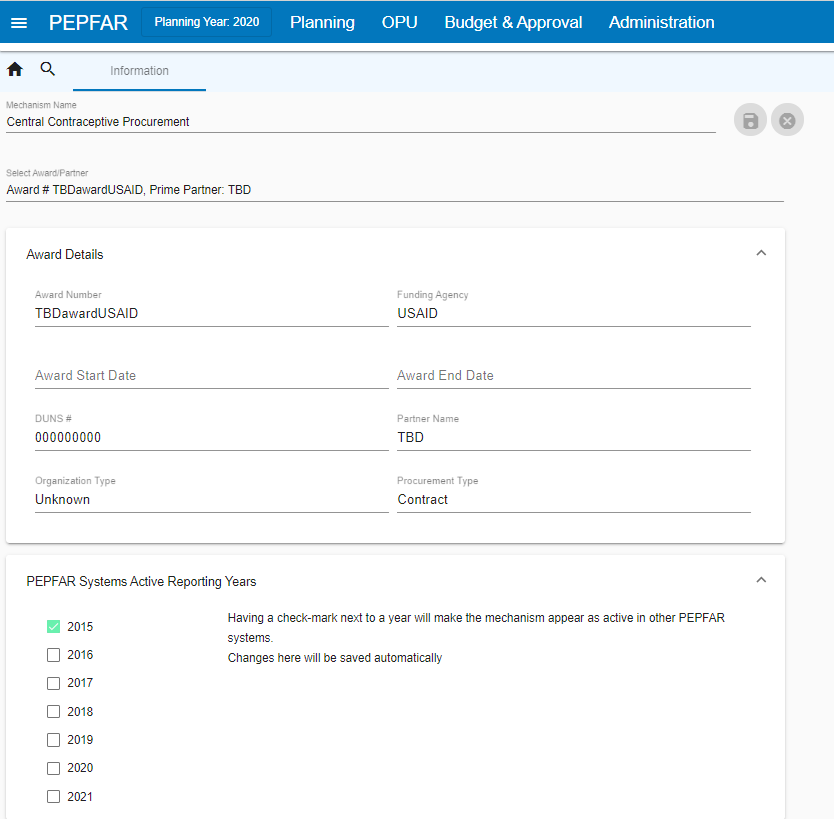
\includegraphics[width=5in]{./images/image15.png}

\end{center}

\hypertarget{note-on-peace-corps-mechanisms}{%
\section{Note on Peace Corps Mechanisms}\label{note-on-peace-corps-mechanisms}}

For the COP21 planning cycle, Peace Corps will transition from reporting
targets under their older mechanisms to reporting all targets under the
Management \& Operations (M\&O) mechanisms. Note that the PSNUxIM tab will
initially populate mechanisms and distributions based on previous year
targets, so users must shift their Peace Corps targets to M\&O mechanisms
from their previous mechanisms by changing the IM reference number at
the top of the tab to the appropriate M\&O IM reference number.

\hypertarget{resolving-rounding-errors}{%
\section{Resolving Rounding Errors}\label{resolving-rounding-errors}}

Due to the combination of multiplication of percentage values against
target values coming from other parts of the DataPack, and rounding of
all mechanism target values to integers, target values allocated against
mechanisms may roll up with some slight difference from DataPack
Targets. It may be necessary to iteratively adjust rounding errors and
deduplications throughout the IM allocation process, though in general
it is a good practice to resolve rounding errors as much as possible
before moving on to deduplication. To resolve rounding errors, adjust
percentages gradually, as follows:

\begin{enumerate}
\def\labelenumi{\arabic{enumi})}
\item
  If you had previously unhid the buffer of green Percentage
  Allocation columns (the section between columns K and CG) while
  adding new mechanisms, or the Deduplication columns in columns CH to
  DB, it may be helpful to hide columns in these sections again now to
  more easily see both Percentage Allocations and Target Values at the
  same time on your screen.
\item
  It may also be helpful to review Duplicated Rollup values in columns
  DC to DE in addition to DataPack Targets in column I so as to
  consider rounding errors distinctly from the impacts of
  deduplication. Note that all when first produced, the PSNUxIM tab
  applies no initial deduplication, so Total Duplicated Rollups and
  DataPack Targets will match when first received.
\item
  While maintaining overall distribution patterns as intended,
  gradually adjust percentage allocations under affected mechanisms in
  columns K through CG to increase or decrease Duplicated Rollups as
  needed.
\end{enumerate}

Note that while all rounding errors should be resolved if possible, a
small margin of error around some values is permissible, so long as this
does not exceed an absolute value of 2 in either direction of the
DataPack Target in column I.

\hypertarget{performing-deduplication}{%
\section{Performing Deduplication}\label{performing-deduplication}}

Follow the below steps to perform all Deduplication associated with IM
allocations of targets. Note that due to improvements to the COP21
DataPack and close alignment with DATIM, performing deduplications in
the DataPack resolves the need to perform any deduplication in DATIM.

\begin{enumerate}
\def\labelenumi{\arabic{enumi}.}
\item
  If you had previously unhid the buffer of green Percentage
  Allocation columns (columns K -- CG), it may be helpful to hide
  empty columns in this section again now.
\item
  Review Duplicated Rollups for DSD, TA, and total targets, beginning
  in column DC. These are dynamically summed across all mechanism
  targets allocated in the PSNU x IM tab to the right of these
  columns. To adjust these totals, return to the Percentage Allocation
  section.
\item
  Review TA Deduplication in columns CV to DB, DSD Deduplication in
  columns CO to CU, and Crosswalk Deduplication in columns CH to CN
  (recommended in that order for each row):

  \begin{enumerate}
  \def\labelenumii{\alph{enumii}.}
  \item
    Where only a single mechanism is assigned targets under either
    DSD or TA (for DSD and TA Deduplication), where deduplicated DSD
    and TA totals (see column CH) aggregate to less than or equal to
    DataPack targets (for Crosswalk Deduplication), or where total
    mechanism targets (column DC) aggregate to less than or equal to
    DataPack Targets (column I), gray highlighting in these sections
    indicates that deduplication is not necessary or permitted.
  \item
    Review allowable ranges for possible deduplicated totals by
    referencing the SUM and MAX rollup columns. As in the DATIM
    Deduplication App, SUM values represent cases with zero
    deduplication, and MAX rollups represent application of the most
    deduplication possible, resulting in values equivalent to the
    largest IM target among either the DSD or TA mechanisms (for DSD
    or TA deduplication), or the larger of either DSD or TA
    deduplicated totals (for crosswalk deduplication).
  \item
    Review Observed Dedupe Resolutions seen in FY21 Target
    allocations. These are provided for reference, and indicate
    which deduplication approach was used in FY21 Target
    deduplication, performed in the DATIM Deduplication App.
  \item
    For cases where Custom deduplication was used in FY21 Targets,
    review the Custom Dedupe Allocation observed in FY21 Targets.
    Percentages here are calculated by dividing the DSD or TA
    deduplication value (for DSD or TA deduplication) or the sum of
    Deduplicated DSD and Deduplicated TA (for crosswalk
    deduplication) by the sum of all mechanisms and deduplication
    values, across both DSD and TA. As such, these values are all
    negative or zero, and can be easily compared against target
    allocation percentages used in columns K -- CG.
  \item
    In columns CZ for TA, CS for DSD, and CL for Crosswalk, manually
    type the deduplication resolution approach to be used to resolve
    deduplication issues, as follows:

    \begin{enumerate}
    \def\labelenumiii{\roman{enumiii}.}
    \item
      ``CUSTOM'' or ``custom'' or ``Custom''
    \item
      ``SUM'' or ``sum'' or ``Sum''
    \item
      ``MAX'' or ``max'' or ``Max''
    \end{enumerate}
  \item
    Where Custom deduplication is selected, also indicate the
    percentage allocation to be assigned to the deduplication value
    in the column to the immediate right. Again, a reminder that
    these values should all be negative or zero, and represent the
    proportion of deduplication values relative to the DataPack
    Target total in column I. Initially upon indicating Custom
    deduplication, the DataPack will preset this deduplication
    allocation equal to the value observed in FY21 Targets, if any.
    You may alter and adjust this value as needed, so long as it is
    negative or zero. Also note that it is not enough to only type
    in a percentage deduplication allocation; you must also enter
    ``CUSTOM'', ``SUM'', or ``MAX'', as explained in the previous step.
    Note that instead of entering ``SUM'', it is possible to enter
    ``CUSTOM'' but enter a deduplication percentage allocation of 0\%;
    and instead of entering ``MAX'', it is possible to enter ``CUSTOM''
    but enter a deduplication percentage allocation that results in
    the equivalent of the MAX value shown in columns CI, CP, or CW.
  \end{enumerate}
\item
  Review the Rollup values in column J for any mismatch against
  DataPack Targets in column I that may necessitate adjustment of
  Deduplication allocations. Note that while it is not a strict
  requirement that percentage allocations across mechanisms and
  deduplication add to 100\%, it is a requirement that integer values
  add to equal the DataPack Target in column I, ± 2. Red highlights in
  column J indicate values more than 2 (integer, absolute value) away
  from the DataPack Targets in column I; yellow highlights indicate
  values 1 or 2 (integer, absolute value) away from the DataPack
  Targets column I.
\end{enumerate}

\elandscape

\newpage

\hypertarget{datapack-self-service-app}{%
\chapter{Datapack Self-service App}\label{datapack-self-service-app}}

The DataPack self-service app provides a one-stop shop for validating
and analyzing your DataPack. After logging into the app, you can upload
a copy of your DataPack, and receive feedback regarding the structure
and content of the DataPack. The app will attempt to provide feedback
regarding any errors which may prevent the import of your DataPack into
DATIM. In general, all errors must be resolved prior to any approval or
import of data into DATIM. Warning messages should be carefully
reviewed. While these may not prevent import of your data, ignoring them
may lead to data quality problems. The app also provides a number of
charts and tables to assist with review of your DataPack. Each of these
functions will be described in more detail in the remained of this
chapter.

\hypertarget{logging-in}{%
\section{Logging in}\label{logging-in}}

In order to access the app, you will need to login with your DATIM
credentials. If you do not have a DATIM username and password or if your
account has been deactivated, please contact DATIM support.

\hypertarget{uploading-a-datapack}{%
\section{Uploading a DataPack}\label{uploading-a-datapack}}

Once you have logged into the app, choose ``Browse'' from the left side
pane. Select the DataPack you wish to validate. Please be sure to use an
``XLSX'' file! Other formats such as XLSB or ZIP archives of your DataPack
are not supported, and cannot be used.

Once you file is completely uploaded to the server, the ``Validate''
button should become active.

\hypertarget{validating-your-datapack}{%
\section{Validating your DataPack}\label{validating-your-datapack}}

After pressing the ``Validate'' button on the left-side pane, the app will
perform a number of structural checks on your file. It is critical that
the structure of the DataPack matches that which was provided to you.
Any tabs or columns which have been removed will result in a parsing
error, and these will need to be fixed prior to import. Other checks
include:

\begin{itemize}
\item
  Altered formulas: Generally, formulas should not be altered, but
  there can be valid programmatic reasons for doing so. These warnings
  are provided in order to allow those reviewing the DataPack to make
  a determination as to whether they are valid changes or not.
\item
  Decimal values: In general, all values (with a few exceptions)
  should be whole integer numbers. Decimals cannot be imported into
  DATIM, and thus must be rounded prior to import. This can lead to
  variations in the numbers which are visible in the DataPack and
  those which are imported into DATIM.
\item
  Negative numbers: In general, all numbers in the DataPack should be
  whole, positive integers.
\item
  Non-numeric values: Any values which are not numeric, e.g.
  characters, is not allowed.
\item
  Imbalanced PSNUxIM distribution: When distributing data from the
  main DataPack tabs, to the PSNUxIM tab, small varations due to
  rounding may result. As an example, if a target of 100 has been set
  in the main tab, and is then distributed evenly between three
  partners, each with a target value of 33, a value of 1 remains
  undistributed. To avoid this situation you may need to use
  allocation targets of 34\%,34\%,32\% instead, which would ensure that
  the values allocated in the PSNUxIM tab match those in the main
  programmatic area tabs.
\item
  Threaded comments: This type of comment, as opposed to the previous
  type of Notes used in Microsoft Excel, causes corruption issues when
  the app attempts to update your PSNUxIM tab. Prior to submitting for
  an updated PSNUxIM tab, you MUST remove all threaded comments. For
  more information about the differences between threaded comments and
  notes visit this
  \href{https://support.office.com/en-us/article/the-difference-between-threaded-comments-and-notes-75a51eec-4092-42ab-abf8-7669077b7be3}{link}.
\item
  Duplicated rows: There should be no duplicated rows in any of the
  main tabs or the PSNUxIM tab.
\item
  Invalid organisation units: All PSNUs referened in the DataPack must
  exist in DATIM.
\item
  Missing metadata: Certain columns such as the PSNU, Indicator code,
  Age, Sex and KeyPop columns must always be present. If any of these
  values is for some reason missing, please find the location of the
  error and fix the issue.
\end{itemize}

\hypertarget{validation-rule-checks}{%
\section{Validation rule checks}\label{validation-rule-checks}}

Validation rules provide additional data quality controls between
certain indicators. As a simple example, the number of persons testing
positive for HIV should be less than or equal to the number of
individuals tested. Under most circumstances, validation rules should
not be violated, but there can be certain programmatic reasons why these
violations should be waived.

A number of rules have been created, and many of them are enforced in
the DataPack itself. However, not all rules have been implemented in the
DataPack, and due to formula changes and subtleties in how targets are
allocated at the PSNUxIM level, additional review of the data in the
PSNUxIM tab and main tabs may be required. During the validation of the
datapack, all data contained in the PSNUxIM tab will be checked against
all of the validation rules defined in DATIM. If there are any
violations of the validation rules, the app will provide detailed
feedback in regards to which PSNUxIM combination is affected. In order
to resolve these, you will need to carefully review how the PNSUxIM
allocations have been made to respective mechanisms in the PSNUxIM tab.

While validation rule violations will not prevent the import of your
data into DATIM, they may lead to data quality problems in both DATIM
and downstream systems such as Panorama and PAW. If there are any
validation rule issues, your PPM and DUIT can be requested to waive
these at their discreation.

\hypertarget{analytics-checks}{%
\section{Analytics checks}\label{analytics-checks}}

Analytics checks provide an additional type of data quality control. As
an example, one analytics check looks for VMMC indeterminate rates
greater than 5 percent. Ideally, the indeterminate rate should be a low
as possible, but if for some reason targets have been set where the rate
is greater than 5 \%, the app will inform you about the specific PSNUxIM
where this occurs. Again, these flags will not prevent the import of
your data into DATIM, but are provided to help reviewers to make a
determination regarding the approval of the DataPack for import.

The app will provide a list of all analytics checks which have been
flagged in the ``Analytics checks'' tab on the right side of the app pane.

\hypertarget{indicator-summary}{%
\section{Indicator summary}\label{indicator-summary}}

This table provides a high-level SNU level summary of indicators from
each of the main tabs of the DataPack. Note, that this data is NOT drawn
from the PSNUxIM tab. This can be a useful first check of your DataPack,
prior to the allocation of the data in the PSNUxIM tab.

\hypertarget{snulevel-summary}{%
\section{SNUlevel summary}\label{snulevel-summary}}

This table listing provides all of the data from each of the main
DataPack tabs summarized by the SNU level.

\hypertarget{validation-rules}{%
\section{Validation rules}\label{validation-rules}}

This tab provides a listing of all validation rule violations, if any.
The table provides the following fields

\begin{itemize}
\item
  PSNU: The specific PSNU where the violation occurs
\item
  Mechanism: The specific mechanism where the violation occurs.
\item
  Formula: The rule is specified with a left side, a right side, and
  an operator. The left and right side correspond to a data element
  (or data elements) located in the PSNUxIM tab. Using a combination
  of filters (PSNU, Mechanism and Data elemement), you should be able
  to locate the specific rows in the PSNUxIM tab which are leading to
  the validation rule violation.
\item
  Diff (\%) : Provides the percentage difference between the left and
  right side.
\item
  Diff (Absolute) : Provides the numeric difference between the left
  and right side.
\end{itemize}

\begin{longtable}[]{@{}
  >{\raggedright\arraybackslash}p{(\columnwidth - 10\tabcolsep) * \real{0.21}}
  >{\raggedright\arraybackslash}p{(\columnwidth - 10\tabcolsep) * \real{0.13}}
  >{\raggedright\arraybackslash}p{(\columnwidth - 10\tabcolsep) * \real{0.15}}
  >{\raggedright\arraybackslash}p{(\columnwidth - 10\tabcolsep) * \real{0.13}}
  >{\raggedright\arraybackslash}p{(\columnwidth - 10\tabcolsep) * \real{0.26}}
  >{\raggedright\arraybackslash}p{(\columnwidth - 10\tabcolsep) * \real{0.13}}@{}}
\toprule
\begin{minipage}[b]{\linewidth}\raggedright
Validation rule
\end{minipage} & \begin{minipage}[b]{\linewidth}\raggedright
PSNU
\end{minipage} & \begin{minipage}[b]{\linewidth}\raggedright
Mechanism
\end{minipage} & \begin{minipage}[b]{\linewidth}\raggedright
Formula
\end{minipage} & \begin{minipage}[b]{\linewidth}\raggedright
Diff (\%) (Absolute)
\end{minipage} & \begin{minipage}[b]{\linewidth}\raggedright
Diff
\end{minipage} \\
\midrule
\endhead
PMTCT\_STAT
(N, DSD,
Age/Sex/
KnownNewResult)
TARGET \textless=
PMTCT\_STAT
(D, DSD,
Age/Sex) TARGET & Namuno & 160448 & 5317 \textless=
5316 & 0.02 & 1 \\
\bottomrule
\end{longtable}

\newpage

\blandscape

\hypertarget{appendix}{%
\chapter{Appendix}\label{appendix}}

\hypertarget{reference-materials}{%
\section{Reference Materials}\label{reference-materials}}

\begin{itemize}
\item
  COP/ROP 2022 Guidance:
  \url{https://www.state.gov/wp-content/uploads/2020/12/PEPFAR-COP21-Guidance-Final.pdf}
\item
  MER Data Validation Rules User Guide:
  \url{https://datim.zendesk.com/hc/en-us/articles/360055112711-MER-Validation-Guide}

  \begin{itemize}
  \tightlist
  \item
    This Document has been designed to communicate all validation
    rules that the DataPack, as well as other COP21 documents, will
    go through in the validation and upload process. A description
    of the validation rules, their definitions and user actions to
    correct any flagged errors can be found in this document.
  \end{itemize}
\item
  Monitoring, Evaluation, and Reporting Indicator Reference Guide
  (MER) v2.5:
  \url{https://datim.zendesk.com/hc/en-us/articles/360000084446-MER-Indicator-Reference-Guides}
\item
  MER 2.5 Training Videos:
  \url{https://datim.zendesk.com/hc/en-us/articles/360051593031-MER-2-5-Training-Videos}
\end{itemize}

\elandscape

\end{document}
